\documentclass[letterpaper]{book}
\usepackage{makeidx}
\usepackage{fancyhdr}
\usepackage{graphicx}
\usepackage{multicol}
\usepackage{float}
\usepackage{textcomp}
\usepackage{alltt}
\usepackage{times}
\ifx\pdfoutput\undefined
\usepackage[ps2pdf,
            pagebackref=true,
            colorlinks=true,
            linkcolor=blue
           ]{hyperref}
\usepackage{pspicture}
\else
\usepackage[pdftex,
            pagebackref=true,
            colorlinks=true,
            linkcolor=blue
           ]{hyperref}
\fi
\usepackage{doxygen}
\makeindex
\setcounter{tocdepth}{1}
\renewcommand{\footrulewidth}{0.4pt}
\begin{document}
\begin{titlepage}
\vspace*{7cm}
\begin{center}
{\Large gemoda Reference Manual}\\
\vspace*{1cm}
{\large Generated by Doxygen 1.4.4}\\
\vspace*{0.5cm}
{\small Fri Mar 3 09:05:14 2006}\\
\end{center}
\end{titlepage}
\clearemptydoublepage
\pagenumbering{roman}
\tableofcontents
\clearemptydoublepage
\pagenumbering{arabic}
\chapter{gemoda Directory Documentation}
\hypertarget{dir_000000}{
\section{Fasta\-Seq\-IO/ Directory Reference}
\label{dir_000000}\index{FastaSeqIO/ Directory Reference@{FastaSeqIO/ Directory Reference}}
}


\begin{figure}[H]
\begin{center}
\leavevmode
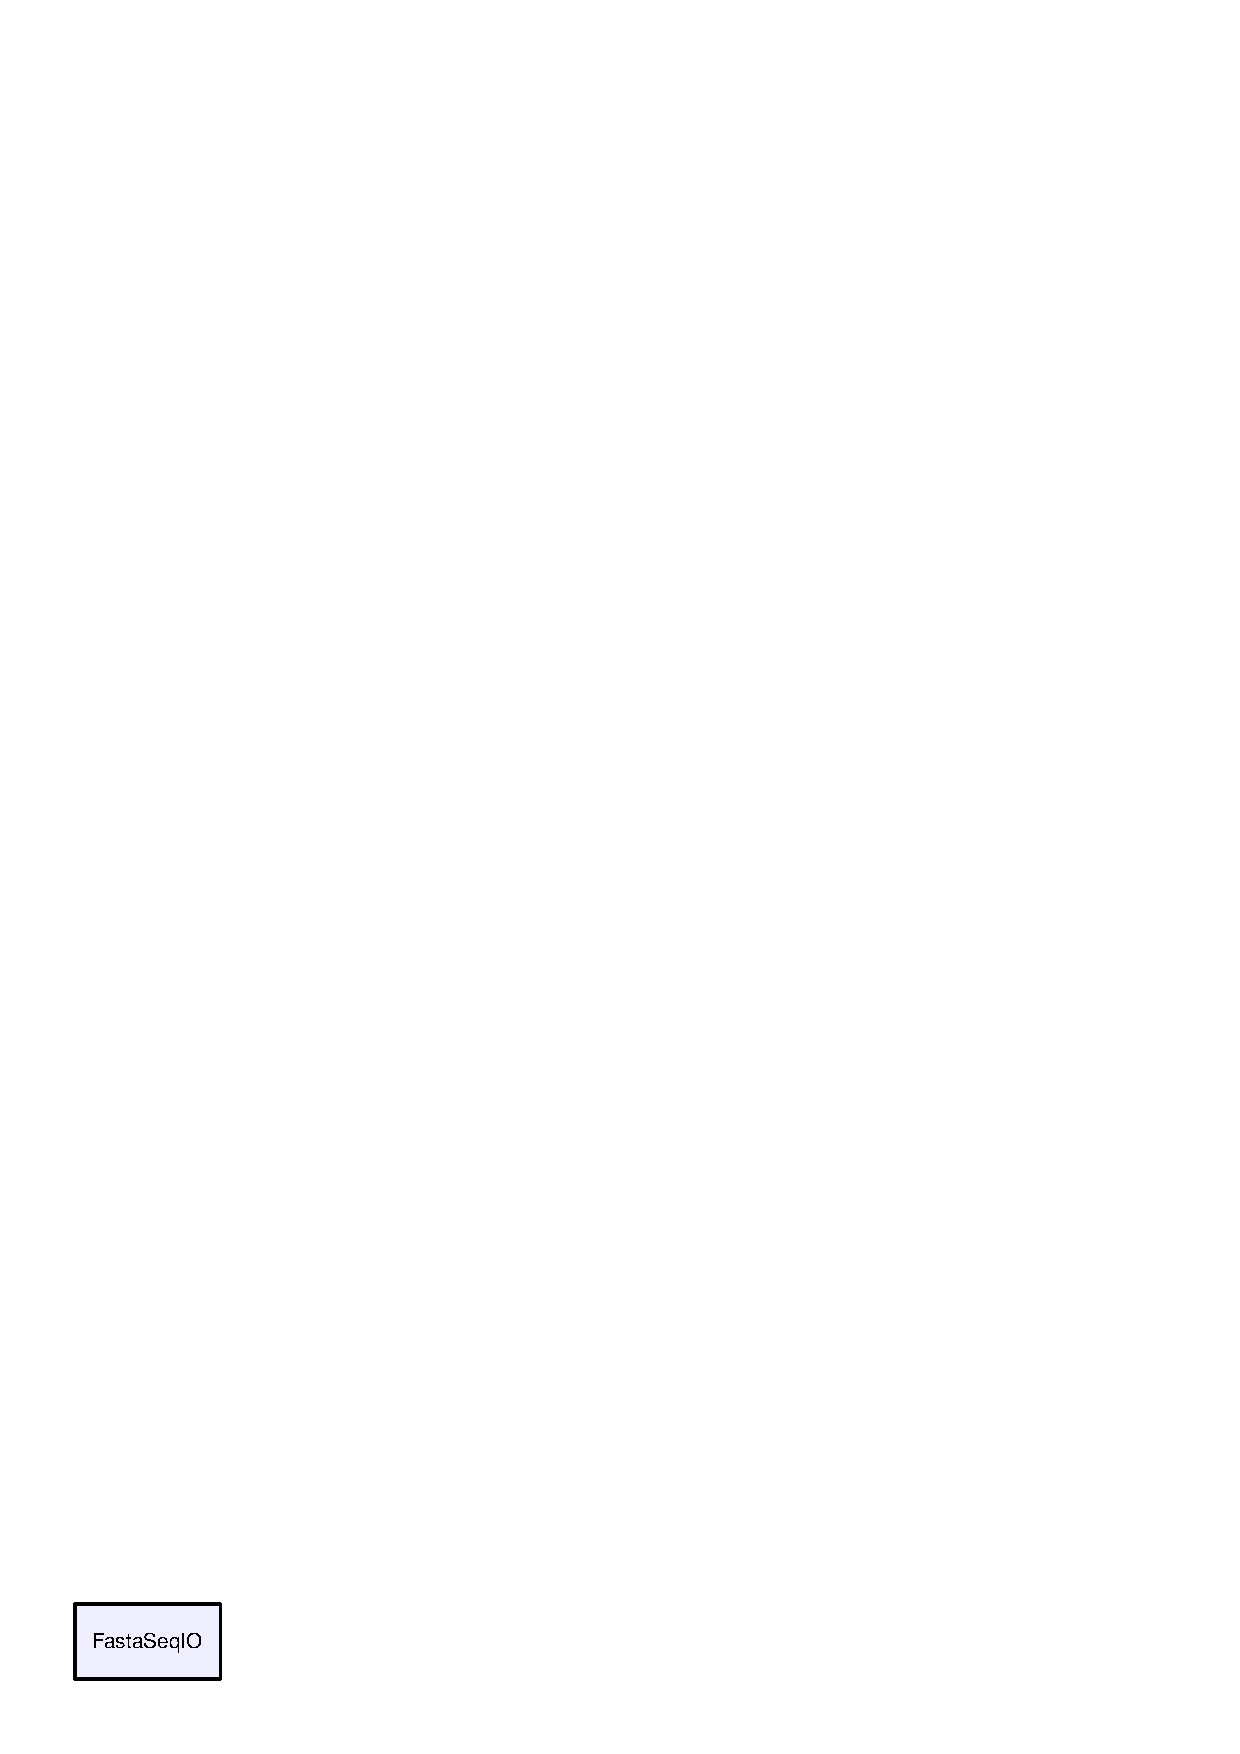
\includegraphics[width=53pt]{dir_000000_dep}
\end{center}
\end{figure}
\subsection*{Files}
\begin{CompactItemize}
\item 
file \hyperlink{fastaSeqIO_8c}{fasta\-Seq\-IO.c}
\item 
file \hyperlink{fastaSeqIO_8h}{fasta\-Seq\-IO.h}
\end{CompactItemize}

\chapter{gemoda Data Structure Documentation}
\hypertarget{structbitGraph__t}{
\section{bit\-Graph\_\-t Struct Reference}
\label{structbitGraph__t}\index{bitGraph_t@{bitGraph\_\-t}}
}
{\tt \#include $<$bit\-Set.h$>$}

Collaboration diagram for bit\-Graph\_\-t:\begin{figure}[H]
\begin{center}
\leavevmode
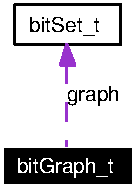
\includegraphics[width=49pt]{structbitGraph__t__coll__graph}
\end{center}
\end{figure}
\subsection*{Data Fields}
\begin{CompactItemize}
\item 
int \hyperlink{structbitGraph__t_o0}{size}
\item 
\hyperlink{structbitSet__t}{bit\-Set\_\-t} $\ast$$\ast$ \hyperlink{structbitGraph__t_o1}{graph}
\end{CompactItemize}


\subsection*{Detailed Description}
A bit graph is an array of bit sets. The graph must be of size size x size. This data structure is used to store adjacency matrices. In particular, a bit graph is used in the clustering step. It can easily be considered a set of sets.



Definition at line 48 of file bit\-Set.h.

\subsection*{Field Documentation}
\hypertarget{structbitGraph__t_o1}{
\index{bitGraph_t@{bit\-Graph\_\-t}!graph@{graph}}
\index{graph@{graph}!bitGraph_t@{bit\-Graph\_\-t}}
\subsubsection[graph]{\setlength{\rightskip}{0pt plus 5cm}\hyperlink{structbitSet__t}{bit\-Set\_\-t}$\ast$$\ast$ \hyperlink{structbitGraph__t_o1}{bit\-Graph\_\-t::graph}}}
\label{structbitGraph__t_o1}


A pointer used to store an array of \hyperlink{structbitSet__t}{bit\-Set\_\-t} space objects.

Definition at line 56 of file bit\-Set.h.

Referenced by bit\-Graph\-Check\-Bit(), bit\-Graph\-Row\-Intersection(), bit\-Graph\-Row\-Union(), bit\-Graph\-Set\-False(), bit\-Graph\-Set\-False\-Diagonal(), bit\-Graph\-Set\-False\-Sym(), bit\-Graph\-Set\-True(), bit\-Graph\-Set\-True\-Diagonal(), bit\-Graph\-Set\-True\-Sym(), copy\-Bit\-Graph(), count\-Bit\-Graph\-Non\-Zero(), delete\-Bit\-Graph(), empty\-Bit\-Graph(), empty\-Bit\-Graph\-Row(), fill\-Bit\-Graph(), filter\-Iter(), find\-Cliques(), get\-Stat\-Mat(), mask\-Bit\-Graph(), new\-Bit\-Graph(), print\-Bit\-Graph(), prune\-Bit\-Graph(), and single\-Linkage().\hypertarget{structbitGraph__t_o0}{
\index{bitGraph_t@{bit\-Graph\_\-t}!size@{size}}
\index{size@{size}!bitGraph_t@{bit\-Graph\_\-t}}
\subsubsection[size]{\setlength{\rightskip}{0pt plus 5cm}int \hyperlink{structbitGraph__t_o0}{bit\-Graph\_\-t::size}}}
\label{structbitGraph__t_o0}


The total size of a bit graph, which is assumed to be symmetric. There are {\em size\/} bit sets in a bit graph, each of size {\em size\/}.

Definition at line 53 of file bit\-Set.h.

Referenced by convolve(), copy\-Bit\-Graph(), filter\-Graph(), find\-Cliques(), get\-Stat\-Mat(), main(), new\-Bit\-Graph(), and old\-Get\-Stat\-Mat().

The documentation for this struct was generated from the following file:\begin{CompactItemize}
\item 
\hyperlink{bitSet_8h}{bit\-Set.h}\end{CompactItemize}

\hypertarget{structbitSet__t}{
\section{bit\-Set\_\-t Struct Reference}
\label{structbitSet__t}\index{bitSet_t@{bitSet\_\-t}}
}
{\tt \#include $<$bit\-Set.h$>$}

\subsection*{Data Fields}
\begin{CompactItemize}
\item 
int \hyperlink{structbitSet__t_o0}{max}
\item 
int \hyperlink{structbitSet__t_o1}{slots}
\item 
int \hyperlink{structbitSet__t_o2}{bytes}
\item 
\hyperlink{bitSet_8h_a9}{bit\_\-t} $\ast$ \hyperlink{structbitSet__t_o3}{tf}
\end{CompactItemize}


\subsection*{Detailed Description}
A bit set is a data structure for storing set objects that allows for quick set operations such as intersections, unions, differences, and so forth. On a standard 32-bit architecture, 32 operations can be performed at the same time, greatly speeding the clique finding stage of the algorithm.



Definition at line 24 of file bit\-Set.h.

\subsection*{Field Documentation}
\hypertarget{structbitSet__t_o2}{
\index{bitSet_t@{bit\-Set\_\-t}!bytes@{bytes}}
\index{bytes@{bytes}!bitSet_t@{bit\-Set\_\-t}}
\subsubsection[bytes]{\setlength{\rightskip}{0pt plus 5cm}int \hyperlink{structbitSet__t_o2}{bit\-Set\_\-t::bytes}}}
\label{structbitSet__t_o2}


This variable actually holds the total number of bits, rather than the number of bytes. However, we chose to keep this name rather than make a variety of changes.

Definition at line 37 of file bit\-Set.h.

Referenced by empty\-Set(), fill\-Set(), and new\-Bit\-Set().\hypertarget{structbitSet__t_o0}{
\index{bitSet_t@{bit\-Set\_\-t}!max@{max}}
\index{max@{max}!bitSet_t@{bit\-Set\_\-t}}
\subsubsection[max]{\setlength{\rightskip}{0pt plus 5cm}int \hyperlink{structbitSet__t_o0}{bit\-Set\_\-t::max}}}
\label{structbitSet__t_o0}


The maximum integer that can be set to true or false.

Definition at line 28 of file bit\-Set.h.

Referenced by new\-Bit\-Set(), next\-Bit\-Bit\-Set(), set\-False(), and set\-True().\hypertarget{structbitSet__t_o1}{
\index{bitSet_t@{bit\-Set\_\-t}!slots@{slots}}
\index{slots@{slots}!bitSet_t@{bit\-Set\_\-t}}
\subsubsection[slots]{\setlength{\rightskip}{0pt plus 5cm}int \hyperlink{structbitSet__t_o1}{bit\-Set\_\-t::slots}}}
\label{structbitSet__t_o1}


The total number of slots, where a slot holds a number of bits equal to the size of a bit\_\-t space object.

Definition at line 32 of file bit\-Set.h.

Referenced by bit\-Set3Way\-Intersection(), bit\-Set\-Difference(), bit\-Set\-Intersection(), bit\-Set\-Sum(), bit\-Set\-Union(), copy\-Set(), and new\-Bit\-Set().\hypertarget{structbitSet__t_o3}{
\index{bitSet_t@{bit\-Set\_\-t}!tf@{tf}}
\index{tf@{tf}!bitSet_t@{bit\-Set\_\-t}}
\subsubsection[tf]{\setlength{\rightskip}{0pt plus 5cm}\hyperlink{bitSet_8h_a9}{bit\_\-t}$\ast$ \hyperlink{structbitSet__t_o3}{bit\-Set\_\-t::tf}}}
\label{structbitSet__t_o3}


A pointer to a bit\_\-t, which is used to store an array of these objects.

Definition at line 40 of file bit\-Set.h.

Referenced by bit\-Set3Way\-Intersection(), bit\-Set\-Difference(), bit\-Set\-Intersection(), bit\-Set\-Sum(), bit\-Set\-Union(), check\-Bit(), copy\-Set(), count\-Set(), delete\-Bit\-Set(), empty\-Set(), fill\-Set(), flip\-Bits(), new\-Bit\-Set(), next\-Bit\-Bit\-Set(), print\-Binary\-Bit\-Set(), set\-False(), and set\-True().

The documentation for this struct was generated from the following file:\begin{CompactItemize}
\item 
\hyperlink{bitSet_8h}{bit\-Set.h}\end{CompactItemize}

\hypertarget{structcnode}{
\section{cnode Struct Reference}
\label{structcnode}\index{cnode@{cnode}}
}
{\tt \#include $<$convll.h$>$}

Collaboration diagram for cnode:\begin{figure}[H]
\begin{center}
\leavevmode
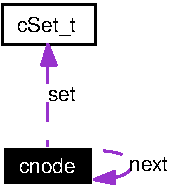
\includegraphics[width=59pt]{structcnode__coll__graph}
\end{center}
\end{figure}
\subsection*{Data Fields}
\begin{CompactItemize}
\item 
\hyperlink{structcSet__t}{c\-Set\_\-t} $\ast$ \hyperlink{structcnode_o0}{set}
\item 
int \hyperlink{structcnode_o1}{id}
\item 
int \hyperlink{structcnode_o2}{length}
\item 
\hyperlink{structcnode}{cnode} $\ast$ \hyperlink{structcnode_o3}{next}
\item 
double \hyperlink{structcnode_o4}{stat}
\end{CompactItemize}


\subsection*{Detailed Description}
This data structure is a linked list for storing cliques. Each member of the linked list has a set, an ID number, a length (which gives the number of characters in the motif), a pointer to the next member of the linked list, and a floating-point number for storing statistical information.



Definition at line 35 of file convll.h.

\subsection*{Field Documentation}
\hypertarget{structcnode_o1}{
\index{cnode@{cnode}!id@{id}}
\index{id@{id}!cnode@{cnode}}
\subsubsection[id]{\setlength{\rightskip}{0pt plus 5cm}int \hyperlink{structcnode_o1}{cnode::id}}}
\label{structcnode_o1}


Identification number for this member. 

Definition at line 38 of file convll.h.

Referenced by add\-To\-Stacks(), print\-Cll(), print\-Cll\-Pattern(), push\-Cll(), remove\-Supers(), single\-Clique\-Conv(), sort\-By\-Stats(), swap\-Nodec\-Set(), uniq\-Clique(), whole\-Clique\-Conv(), whole\-Round\-Conv(), and yank\-Cll().\hypertarget{structcnode_o2}{
\index{cnode@{cnode}!length@{length}}
\index{length@{length}!cnode@{cnode}}
\subsubsection[length]{\setlength{\rightskip}{0pt plus 5cm}int \hyperlink{structcnode_o2}{cnode::length}}}
\label{structcnode_o2}


Length of this motif. 

Definition at line 41 of file convll.h.

Referenced by calc\-Stat\-Cliq(), get\-Largest\-Length(), main(), output\-Real\-Pats(), output\-Real\-Pats\-WCentroid(), print\-Cll(), and push\-Cll().\hypertarget{structcnode_o3}{
\index{cnode@{cnode}!next@{next}}
\index{next@{next}!cnode@{cnode}}
\subsubsection[next]{\setlength{\rightskip}{0pt plus 5cm}struct \hyperlink{structcnode}{cnode}$\ast$ \hyperlink{structcnode_o3}{cnode::next}}}
\label{structcnode_o3}


A pointer to the next member, or the next motif. 

Definition at line 42 of file convll.h.

Referenced by calc\-Stat\-All\-Cliqs(), fill\-Member\-Stacks(), get\-Largest\-Length(), get\-Largest\-Support(), main(), output\-Real\-Pats(), output\-Real\-Pats\-WCentroid(), pop\-Cll(), print\-Cll(), prune\-Cll(), push\-Cll(), remove\-Supers(), single\-Clique\-Conv(), sort\-By\-Stats(), swap\-Nodec\-Set(), uniq\-Clique(), whole\-Round\-Conv(), and yank\-Cll().\hypertarget{structcnode_o0}{
\index{cnode@{cnode}!set@{set}}
\index{set@{set}!cnode@{cnode}}
\subsubsection[set]{\setlength{\rightskip}{0pt plus 5cm}\hyperlink{structcSet__t}{c\-Set\_\-t}$\ast$ \hyperlink{structcnode_o0}{cnode::set}}}
\label{structcnode_o0}


The set for this member of the linked list. 

Definition at line 37 of file convll.h.

Referenced by add\-To\-Stacks(), calc\-Stat\-Cliq(), find\-Clique\-Centroid(), get\-Largest\-Support(), inithead\-Cll(), main(), make\-Alternate\-Centroid(), merge\-Intersect(), output\-Real\-Pats(), output\-Real\-Pats\-WCentroid(), pop\-Cll(), print\-Cll(), print\-Cll\-Pattern(), prune\-Cll(), push\-Cll(), remove\-Supers(), single\-Clique\-Conv(), swap\-Nodec\-Set(), uniq\-Clique(), and whole\-Clique\-Conv().\hypertarget{structcnode_o4}{
\index{cnode@{cnode}!stat@{stat}}
\index{stat@{stat}!cnode@{cnode}}
\subsubsection[stat]{\setlength{\rightskip}{0pt plus 5cm}double \hyperlink{structcnode_o4}{cnode::stat}}}
\label{structcnode_o4}


Used to store the statistical store of a motif. 

Definition at line 43 of file convll.h.

Referenced by calc\-Stat\-All\-Cliqs(), main(), output\-Real\-Pats(), and push\-Cll().

The documentation for this struct was generated from the following file:\begin{CompactItemize}
\item 
\hyperlink{convll_8h}{convll.h}\end{CompactItemize}

\hypertarget{structcSet__t}{
\section{c\-Set\_\-t Struct Reference}
\label{structcSet__t}\index{cSet_t@{cSet\_\-t}}
}
{\tt \#include $<$convll.h$>$}

\subsection*{Data Fields}
\begin{CompactItemize}
\item 
int \hyperlink{structcSet__t_o0}{size}
\item 
int $\ast$ \hyperlink{structcSet__t_o1}{members}
\end{CompactItemize}


\subsection*{Detailed Description}
A c\-Set\_\-t is used to hold a set of integers, in cases where the upper limit of integers size is unknown. Or, in cases where using a bit set would be impractical. This data structure is used throughout the convolution, where we have found heuristically that intersections of this data type are much faster than those for bit\-Set\_\-t's, which would require a bit shift.



Definition at line 21 of file convll.h.

\subsection*{Field Documentation}
\hypertarget{structcSet__t_o1}{
\index{cSet_t@{c\-Set\_\-t}!members@{members}}
\index{members@{members}!cSet_t@{c\-Set\_\-t}}
\subsubsection[members]{\setlength{\rightskip}{0pt plus 5cm}int$\ast$ \hyperlink{structcSet__t_o1}{c\-Set\_\-t::members}}}
\label{structcSet__t_o1}


Array of pointers to ints that holds the members of this set. 

Definition at line 26 of file convll.h.

Referenced by add\-To\-Stacks(), bit\-Set\-To\-CSet(), check\-Cliquec\-Set(), find\-Clique\-Centroid(), main(), make\-Alternate\-Centroid(), merge\-Intersect(), mll\-To\-CSet(), output\-Real\-Pats(), output\-Real\-Pats\-WCentroid(), pop\-Cll(), print\-Cll(), print\-Cll\-Pattern(), print\-CSet(), prune\-Cll(), push\-Conv\-Clique(), remove\-Supers(), swap\-Nodec\-Set(), uniq\-Clique(), and whole\-Clique\-Conv().\hypertarget{structcSet__t_o0}{
\index{cSet_t@{c\-Set\_\-t}!size@{size}}
\index{size@{size}!cSet_t@{c\-Set\_\-t}}
\subsubsection[size]{\setlength{\rightskip}{0pt plus 5cm}int \hyperlink{structcSet__t_o0}{c\-Set\_\-t::size}}}
\label{structcSet__t_o0}


Number of members in this set. 

Definition at line 24 of file convll.h.

Referenced by bit\-Set\-To\-CSet(), calc\-Stat\-Cliq(), check\-Cliquec\-Set(), find\-Clique\-Centroid(), get\-Largest\-Support(), main(), mll\-To\-CSet(), output\-Real\-Pats(), output\-Real\-Pats\-WCentroid(), print\-Cll(), print\-Cll\-Pattern(), print\-CSet(), prune\-Cll(), remove\-Supers(), single\-Clique\-Conv(), uniq\-Clique(), and whole\-Clique\-Conv().

The documentation for this struct was generated from the following file:\begin{CompactItemize}
\item 
\hyperlink{convll_8h}{convll.h}\end{CompactItemize}

\hypertarget{structfSeq__t}{
\section{f\-Seq\_\-t Struct Reference}
\label{structfSeq__t}\index{fSeq_t@{fSeq\_\-t}}
}
{\tt \#include $<$fasta\-Seq\-IO.h$>$}

\subsection*{Data Fields}
\begin{CompactItemize}
\item 
char $\ast$ \hyperlink{structfSeq__t_o0}{seq}
\item 
char $\ast$ \hyperlink{structfSeq__t_o1}{label}
\end{CompactItemize}


\subsection*{Detailed Description}




Definition at line 12 of file fasta\-Seq\-IO.h.

\subsection*{Field Documentation}
\hypertarget{structfSeq__t_o1}{
\index{fSeq_t@{f\-Seq\_\-t}!label@{label}}
\index{label@{label}!fSeq_t@{f\-Seq\_\-t}}
\subsubsection[label]{\setlength{\rightskip}{0pt plus 5cm}char$\ast$ \hyperlink{structfSeq__t_o1}{f\-Seq\_\-t::label}}}
\label{structfSeq__t_o1}




Definition at line 14 of file fasta\-Seq\-IO.h.

Referenced by Free\-FSeqs(), init\-Aof\-FSeqs(), and Read\-FSeqs().\hypertarget{structfSeq__t_o0}{
\index{fSeq_t@{f\-Seq\_\-t}!seq@{seq}}
\index{seq@{seq}!fSeq_t@{f\-Seq\_\-t}}
\subsubsection[seq]{\setlength{\rightskip}{0pt plus 5cm}char$\ast$ \hyperlink{structfSeq__t_o0}{f\-Seq\_\-t::seq}}}
\label{structfSeq__t_o0}




Definition at line 13 of file fasta\-Seq\-IO.h.

Referenced by Free\-FSeqs(), init\-Aof\-FSeqs(), print\-FSeq\-Sub\-Seq(), Read\-FSeqs(), and Read\-Txt\-Seqs().

The documentation for this struct was generated from the following file:\begin{CompactItemize}
\item 
Fasta\-Seq\-IO/\hyperlink{fastaSeqIO_8h}{fasta\-Seq\-IO.h}\end{CompactItemize}

\hypertarget{structmnode}{
\section{mnode Struct Reference}
\label{structmnode}\index{mnode@{mnode}}
}
{\tt \#include $<$convll.h$>$}

Collaboration diagram for mnode:\begin{figure}[H]
\begin{center}
\leavevmode
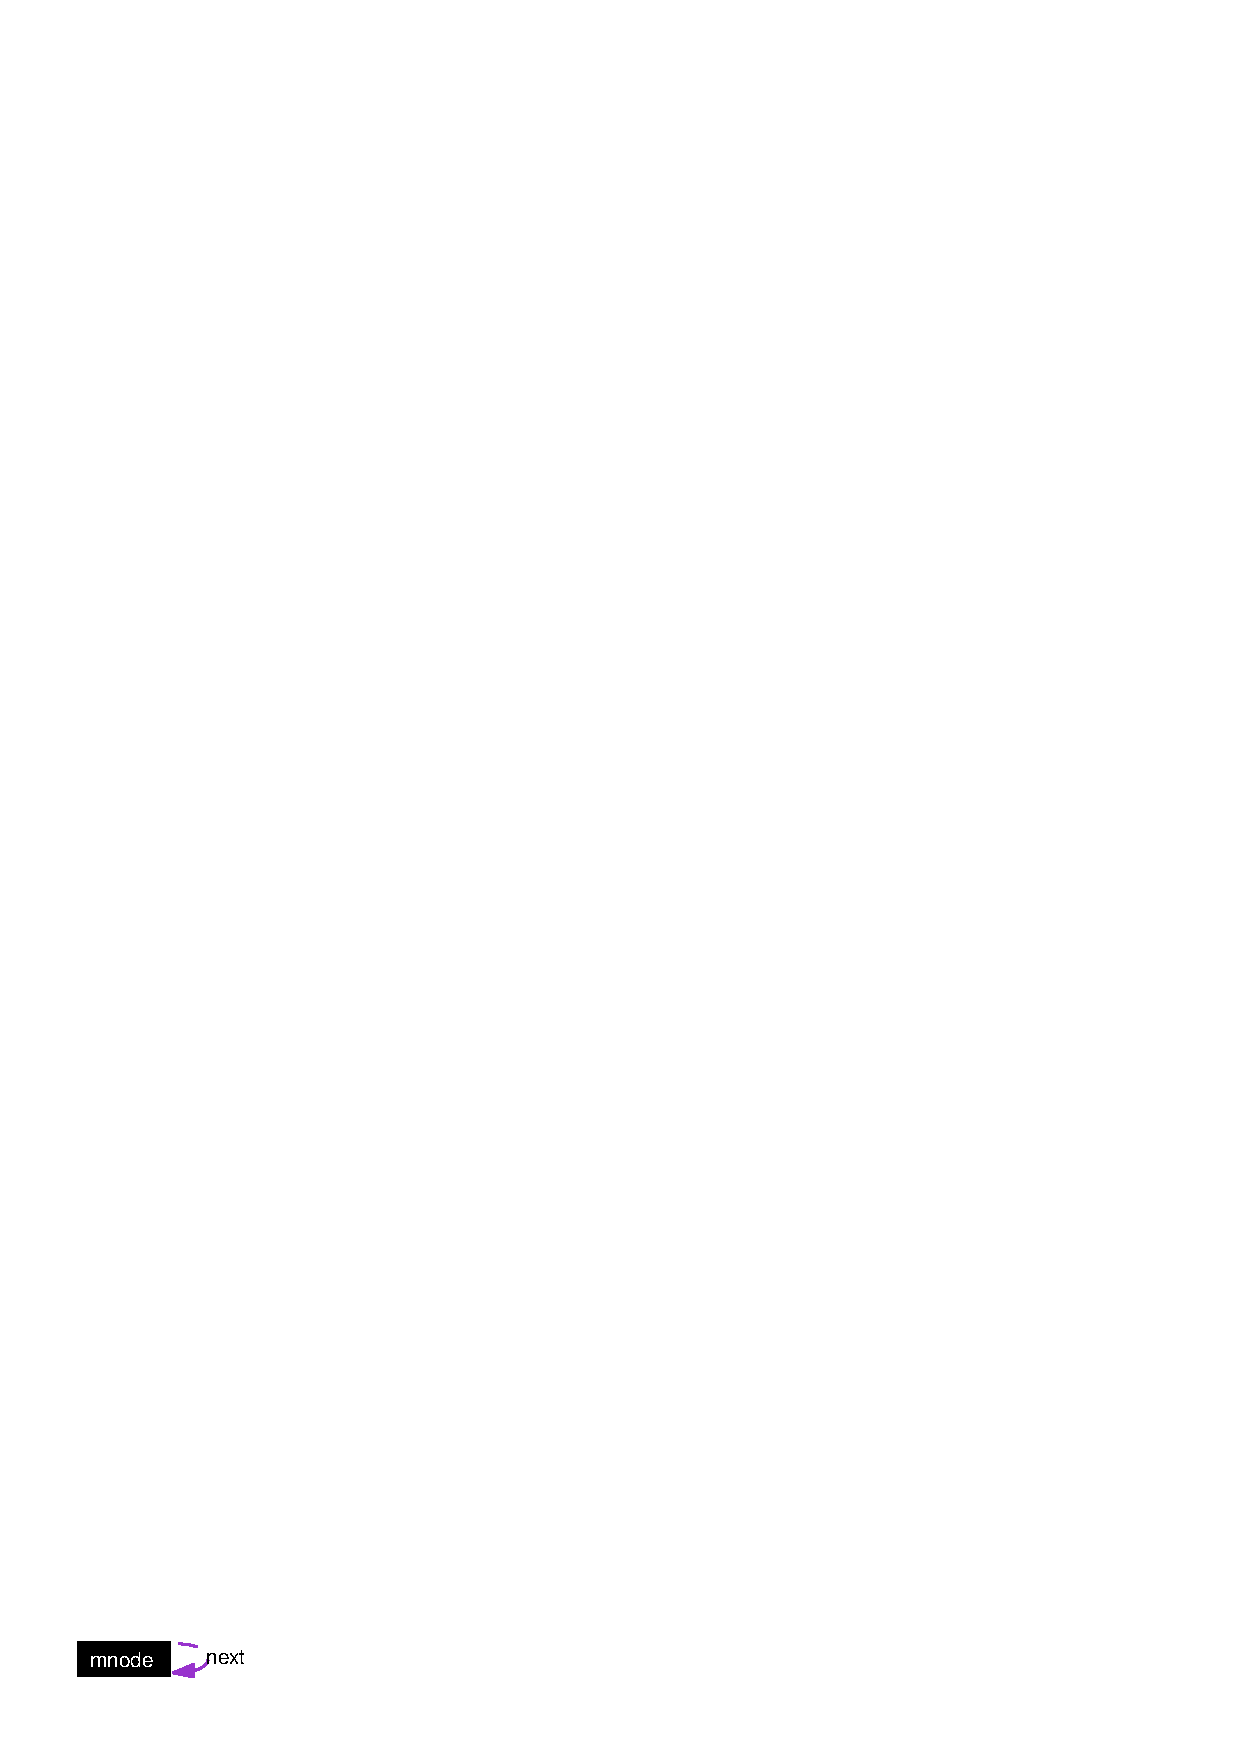
\includegraphics[width=60pt]{structmnode__coll__graph}
\end{center}
\end{figure}
\subsection*{Data Fields}
\begin{CompactItemize}
\item 
int \hyperlink{structmnode_o0}{clique\-Membership}
\item 
\hyperlink{structmnode}{mnode} $\ast$ \hyperlink{structmnode_o1}{next}
\end{CompactItemize}


\subsection*{Detailed Description}
This data structure is just a link to list of integers used for bookkeeping during the convolution stage.



Definition at line 49 of file convll.h.

\subsection*{Field Documentation}
\hypertarget{structmnode_o0}{
\index{mnode@{mnode}!cliqueMembership@{cliqueMembership}}
\index{cliqueMembership@{cliqueMembership}!mnode@{mnode}}
\subsubsection[cliqueMembership]{\setlength{\rightskip}{0pt plus 5cm}int \hyperlink{structmnode_o0}{mnode::clique\-Membership}}}
\label{structmnode_o0}


Clique to which this belongs. 

Definition at line 52 of file convll.h.

Referenced by mll\-To\-CSet(), print\-Member\-Stacks(), push\-Mem\-Stack(), and set\-Stack\-True().\hypertarget{structmnode_o1}{
\index{mnode@{mnode}!next@{next}}
\index{next@{next}!mnode@{mnode}}
\subsubsection[next]{\setlength{\rightskip}{0pt plus 5cm}struct \hyperlink{structmnode}{mnode}$\ast$ \hyperlink{structmnode_o1}{mnode::next}}}
\label{structmnode_o1}


A pointer to the next member in the linked list of mll\_\-t space objects. 

Definition at line 55 of file convll.h.

Referenced by mll\-To\-CSet(), pop\-Mem\-Stack(), print\-Member\-Stacks(), push\-Mem\-Stack(), and set\-Stack\-True().

The documentation for this struct was generated from the following file:\begin{CompactItemize}
\item 
\hyperlink{convll_8h}{convll.h}\end{CompactItemize}

\hypertarget{structrdh__t}{
\section{rdh\_\-t Struct Reference}
\label{structrdh__t}\index{rdh_t@{rdh\_\-t}}
}
{\tt \#include $<$real\-Io.h$>$}

\subsection*{Data Fields}
\begin{CompactItemize}
\item 
int \hyperlink{structrdh__t_o0}{size}
\item 
int \hyperlink{structrdh__t_o1}{index\-Size}
\item 
char $\ast$$\ast$ \hyperlink{structrdh__t_o2}{label}
\item 
gsl\_\-matrix $\ast$$\ast$ \hyperlink{structrdh__t_o3}{seq}
\item 
int $\ast$ \hyperlink{structrdh__t_o4}{index\-To\-Seq}
\item 
int $\ast$ \hyperlink{structrdh__t_o5}{index\-To\-Pos}
\item 
int $\ast$$\ast$ \hyperlink{structrdh__t_o6}{offset\-To\-Index}
\end{CompactItemize}


\subsection*{Detailed Description}
This is a data structure, which is used to store real valued data. Basically, this is an array of gsl\_\-matrix objects, where each matrix represents a single, multidimensional array that was read in from a Fast\-A formatted file.



Definition at line 24 of file real\-Io.h.

\subsection*{Field Documentation}
\hypertarget{structrdh__t_o1}{
\index{rdh_t@{rdh\_\-t}!indexSize@{indexSize}}
\index{indexSize@{indexSize}!rdh_t@{rdh\_\-t}}
\subsubsection[indexSize]{\setlength{\rightskip}{0pt plus 5cm}int \hyperlink{structrdh__t_o1}{rdh\_\-t::index\-Size}}}
\label{structrdh__t_o1}


The size of the index, where the index is used to store pointers to the different sequences in this object. 

Definition at line 30 of file real\-Io.h.

Referenced by get\-Rdh\-Index\-Seq\-Pos(), init\-Rdh(), init\-Rdh\-Index(), real\-Comparison(), and set\-Rdh\-Index().\hypertarget{structrdh__t_o5}{
\index{rdh_t@{rdh\_\-t}!indexToPos@{indexToPos}}
\index{indexToPos@{indexToPos}!rdh_t@{rdh\_\-t}}
\subsubsection[indexToPos]{\setlength{\rightskip}{0pt plus 5cm}int$\ast$ \hyperlink{structrdh__t_o5}{rdh\_\-t::index\-To\-Pos}}}
\label{structrdh__t_o5}


The array of integers that tell us to which position in a sequence each index in the gsl\_\-matrix array corresponds. 

Definition at line 40 of file real\-Io.h.

Referenced by free\-Rdh(), get\-Rdh\-Index\-Seq\-Pos(), init\-Rdh(), init\-Rdh\-Index(), and set\-Rdh\-Index().\hypertarget{structrdh__t_o4}{
\index{rdh_t@{rdh\_\-t}!indexToSeq@{indexToSeq}}
\index{indexToSeq@{indexToSeq}!rdh_t@{rdh\_\-t}}
\subsubsection[indexToSeq]{\setlength{\rightskip}{0pt plus 5cm}int$\ast$ \hyperlink{structrdh__t_o4}{rdh\_\-t::index\-To\-Seq}}}
\label{structrdh__t_o4}


The array of integers that will tell us to which sequence each index and the gsl\_\-matrix array corresponds. 

Definition at line 37 of file real\-Io.h.

Referenced by free\-Rdh(), get\-Rdh\-Index\-Seq\-Pos(), init\-Rdh(), init\-Rdh\-Index(), main(), and set\-Rdh\-Index().\hypertarget{structrdh__t_o2}{
\index{rdh_t@{rdh\_\-t}!label@{label}}
\index{label@{label}!rdh_t@{rdh\_\-t}}
\subsubsection[label]{\setlength{\rightskip}{0pt plus 5cm}char$\ast$$\ast$ \hyperlink{structrdh__t_o2}{rdh\_\-t::label}}}
\label{structrdh__t_o2}


The array of labels that store the names of each sequence. 

Definition at line 32 of file real\-Io.h.

Referenced by free\-Rdh(), get\-Rdh\-Label(), init\-Rdh(), and set\-Rdh\-Label().\hypertarget{structrdh__t_o6}{
\index{rdh_t@{rdh\_\-t}!offsetToIndex@{offsetToIndex}}
\index{offsetToIndex@{offsetToIndex}!rdh_t@{rdh\_\-t}}
\subsubsection[offsetToIndex]{\setlength{\rightskip}{0pt plus 5cm}int$\ast$$\ast$ \hyperlink{structrdh__t_o6}{rdh\_\-t::offset\-To\-Index}}}
\label{structrdh__t_o6}


The array that points from a particular offset to its index. 

Definition at line 42 of file real\-Io.h.

Referenced by free\-Rdh(), init\-Rdh\-Index(), and main().\hypertarget{structrdh__t_o3}{
\index{rdh_t@{rdh\_\-t}!seq@{seq}}
\index{seq@{seq}!rdh_t@{rdh\_\-t}}
\subsubsection[seq]{\setlength{\rightskip}{0pt plus 5cm}gsl\_\-matrix$\ast$$\ast$ \hyperlink{structrdh__t_o3}{rdh\_\-t::seq}}}
\label{structrdh__t_o3}


The array of matrices that store the data we read in. 

Definition at line 34 of file real\-Io.h.

Referenced by free\-Rdh(), general\-Match\-Factor(), get\-Rdh\-Dim(), get\-Rdh\-Seq\-Length(), get\-Rdh\-Value(), init\-Rdh(), init\-Rdh\-Gsl\-Mat(), mass\-Spec\-Compare\-WElut(), output\-Real\-Pats(), rmsd\-Compare(), set\-Rdh\-Col\-From\-String(), set\-Rdh\-Label(), and set\-Rdh\-Value().\hypertarget{structrdh__t_o0}{
\index{rdh_t@{rdh\_\-t}!size@{size}}
\index{size@{size}!rdh_t@{rdh\_\-t}}
\subsubsection[size]{\setlength{\rightskip}{0pt plus 5cm}int \hyperlink{structrdh__t_o0}{rdh\_\-t::size}}}
\label{structrdh__t_o0}


The number of sequences stored in this data structure. 

Definition at line 27 of file real\-Io.h.

Referenced by init\-Rdh(), init\-Rdh\-Index(), and main().

The documentation for this struct was generated from the following file:\begin{CompactItemize}
\item 
\hyperlink{realIo_8h}{real\-Io.h}\end{CompactItemize}

\hypertarget{structsHash__t}{
\section{s\-Hash\_\-t Struct Reference}
\label{structsHash__t}\index{sHash_t@{sHash\_\-t}}
}
Collaboration diagram for s\-Hash\_\-t:\begin{figure}[H]
\begin{center}
\leavevmode
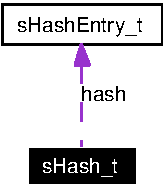
\includegraphics[width=56pt]{structsHash__t__coll__graph}
\end{center}
\end{figure}
\subsection*{Data Fields}
\begin{CompactItemize}
\item 
int $\ast$ \hyperlink{structsHash__t_o0}{hash\-Size}
\item 
int $\ast$ \hyperlink{structsHash__t_o1}{i\-Hash\-Size}
\item 
int \hyperlink{structsHash__t_o2}{total\-Size}
\item 
\hyperlink{structsHashEntry__t}{s\-Hash\-Entry\_\-t} $\ast$$\ast$ \hyperlink{structsHash__t_o3}{hash}
\end{CompactItemize}


\subsection*{Detailed Description}
A data structure for a hash table. At its root, this structure is just an array of hash entry objects. As well, there are members used to track the size of the hash table.



Definition at line 132 of file words.c.

\subsection*{Field Documentation}
\hypertarget{structsHash__t_o3}{
\index{sHash_t@{s\-Hash\_\-t}!hash@{hash}}
\index{hash@{hash}!sHash_t@{s\-Hash\_\-t}}
\subsubsection[hash]{\setlength{\rightskip}{0pt plus 5cm}\hyperlink{structsHashEntry__t}{s\-Hash\-Entry\_\-t}$\ast$$\ast$ \hyperlink{structsHash__t_o3}{s\-Hash\_\-t::hash}}}
\label{structsHash__t_o3}


An array \hyperlink{structsHashEntry__t}{s\-Hash\-Entry\_\-t} space objects. 

Definition at line 148 of file words.c.

Referenced by destroy\-SHash(), print\-SHash(), and search\-SHash().\hypertarget{structsHash__t_o0}{
\index{sHash_t@{s\-Hash\_\-t}!hashSize@{hashSize}}
\index{hashSize@{hashSize}!sHash_t@{s\-Hash\_\-t}}
\subsubsection[hashSize]{\setlength{\rightskip}{0pt plus 5cm}int$\ast$ \hyperlink{structsHash__t_o0}{s\-Hash\_\-t::hash\-Size}}}
\label{structsHash__t_o0}


A pointer to an integer that is used to store an array of integers that keep track of the number of \hyperlink{structsHashEntry__t}{s\-Hash\-Entry\_\-t} objects that are hashed to a particular integer. 

Definition at line 138 of file words.c.

Referenced by destroy\-SHash(), and search\-SHash().\hypertarget{structsHash__t_o1}{
\index{sHash_t@{s\-Hash\_\-t}!iHashSize@{iHashSize}}
\index{iHashSize@{iHashSize}!sHash_t@{s\-Hash\_\-t}}
\subsubsection[iHashSize]{\setlength{\rightskip}{0pt plus 5cm}int$\ast$ \hyperlink{structsHash__t_o1}{s\-Hash\_\-t::i\-Hash\-Size}}}
\label{structsHash__t_o1}


A pointer to an integer that is used to store an array of integers that keep track of the number of \hyperlink{structsHashEntry__t}{s\-Hash\-Entry\_\-t} objects that are hashed to a particular integer. 

Definition at line 143 of file words.c.

Referenced by destroy\-SHash(), and search\-SHash().\hypertarget{structsHash__t_o2}{
\index{sHash_t@{s\-Hash\_\-t}!totalSize@{totalSize}}
\index{totalSize@{totalSize}!sHash_t@{s\-Hash\_\-t}}
\subsubsection[totalSize]{\setlength{\rightskip}{0pt plus 5cm}int \hyperlink{structsHash__t_o2}{s\-Hash\_\-t::total\-Size}}}
\label{structsHash__t_o2}


An integer that stores the total number of slots available in our hash. 

Definition at line 146 of file words.c.

Referenced by init\-SHash(), and search\-SHash().

The documentation for this struct was generated from the following file:\begin{CompactItemize}
\item 
\hyperlink{words_8c}{words.c}\end{CompactItemize}

\hypertarget{structsHashEntry__t}{
\section{s\-Hash\-Entry\_\-t Struct Reference}
\label{structsHashEntry__t}\index{sHashEntry_t@{sHashEntry\_\-t}}
}
\subsection*{Data Fields}
\begin{CompactItemize}
\item 
char $\ast$ \hyperlink{structsHashEntry__t_o0}{key}
\item 
int \hyperlink{structsHashEntry__t_o1}{L}
\item 
int \hyperlink{structsHashEntry__t_o2}{data}
\item 
int \hyperlink{structsHashEntry__t_o3}{idx}
\end{CompactItemize}


\subsection*{Detailed Description}
Type for a hash table entry. This datatype is used to populate a hash table. The most important members of this data structure are the string, or the key, and the index to which that key hashes.



Definition at line 114 of file words.c.

\subsection*{Field Documentation}
\hypertarget{structsHashEntry__t_o2}{
\index{sHashEntry_t@{s\-Hash\-Entry\_\-t}!data@{data}}
\index{data@{data}!sHashEntry_t@{s\-Hash\-Entry\_\-t}}
\subsubsection[data]{\setlength{\rightskip}{0pt plus 5cm}int \hyperlink{structsHashEntry__t_o2}{s\-Hash\-Entry\_\-t::data}}}
\label{structsHashEntry__t_o2}


A throw away variable, used to store any necessary data 

Definition at line 121 of file words.c.

Referenced by count\-Words2(), and print\-SHash().\hypertarget{structsHashEntry__t_o3}{
\index{sHashEntry_t@{s\-Hash\-Entry\_\-t}!idx@{idx}}
\index{idx@{idx}!sHashEntry_t@{s\-Hash\-Entry\_\-t}}
\subsubsection[idx]{\setlength{\rightskip}{0pt plus 5cm}int \hyperlink{structsHashEntry__t_o3}{s\-Hash\-Entry\_\-t::idx}}}
\label{structsHashEntry__t_o3}


The integer to which the {\em key\/} of length {\em L\/} hashes 

Definition at line 123 of file words.c.

Referenced by count\-Words2().\hypertarget{structsHashEntry__t_o0}{
\index{sHashEntry_t@{s\-Hash\-Entry\_\-t}!key@{key}}
\index{key@{key}!sHashEntry_t@{s\-Hash\-Entry\_\-t}}
\subsubsection[key]{\setlength{\rightskip}{0pt plus 5cm}char$\ast$ \hyperlink{structsHashEntry__t_o0}{s\-Hash\-Entry\_\-t::key}}}
\label{structsHashEntry__t_o0}


A pointer to a string 

Definition at line 117 of file words.c.

Referenced by count\-Words2(), print\-SHash(), and search\-SHash().\hypertarget{structsHashEntry__t_o1}{
\index{sHashEntry_t@{s\-Hash\-Entry\_\-t}!L@{L}}
\index{L@{L}!sHashEntry_t@{s\-Hash\-Entry\_\-t}}
\subsubsection[L]{\setlength{\rightskip}{0pt plus 5cm}int \hyperlink{structsHashEntry__t_o1}{s\-Hash\-Entry\_\-t::L}}}
\label{structsHashEntry__t_o1}


The length of the string that should be used to compute the hash 

Definition at line 119 of file words.c.

Referenced by count\-Words2(), print\-SHash(), and search\-SHash().

The documentation for this struct was generated from the following file:\begin{CompactItemize}
\item 
\hyperlink{words_8c}{words.c}\end{CompactItemize}

\hypertarget{structsOffset__t}{
\section{s\-Offset\_\-t Struct Reference}
\label{structsOffset__t}\index{sOffset_t@{sOffset\_\-t}}
}
{\tt \#include $<$spat.h$>$}

\subsection*{Data Fields}
\begin{CompactItemize}
\item 
int \hyperlink{structsOffset__t_o0}{seq}
\item 
int \hyperlink{structsOffset__t_o1}{pos}
\item 
int \hyperlink{structsOffset__t_o2}{next}
\item 
int \hyperlink{structsOffset__t_o3}{prev}
\end{CompactItemize}


\subsection*{Detailed Description}
This object is used to store the location of a particular word and a set of sequences. That is if we hash a word, we would like to know where it came from. This data structure provides that information.



Definition at line 13 of file spat.h.

\subsection*{Field Documentation}
\hypertarget{structsOffset__t_o2}{
\index{sOffset_t@{s\-Offset\_\-t}!next@{next}}
\index{next@{next}!sOffset_t@{s\-Offset\_\-t}}
\subsubsection[next]{\setlength{\rightskip}{0pt plus 5cm}int \hyperlink{structsOffset__t_o2}{s\-Offset\_\-t::next}}}
\label{structsOffset__t_o2}


The index of the word that follows this word at {\em pos\/} plus 1.

Definition at line 23 of file spat.h.

Referenced by count\-Words2().\hypertarget{structsOffset__t_o1}{
\index{sOffset_t@{s\-Offset\_\-t}!pos@{pos}}
\index{pos@{pos}!sOffset_t@{s\-Offset\_\-t}}
\subsubsection[pos]{\setlength{\rightskip}{0pt plus 5cm}int \hyperlink{structsOffset__t_o1}{s\-Offset\_\-t::pos}}}
\label{structsOffset__t_o1}


The position in the sequence where the word is located.

Definition at line 20 of file spat.h.

Referenced by count\-Words2(), and main().\hypertarget{structsOffset__t_o3}{
\index{sOffset_t@{s\-Offset\_\-t}!prev@{prev}}
\index{prev@{prev}!sOffset_t@{s\-Offset\_\-t}}
\subsubsection[prev]{\setlength{\rightskip}{0pt plus 5cm}int \hyperlink{structsOffset__t_o3}{s\-Offset\_\-t::prev}}}
\label{structsOffset__t_o3}


The index of the word that precedes this word at {\em pos\/} minus 1.

Definition at line 26 of file spat.h.

Referenced by count\-Words2().\hypertarget{structsOffset__t_o0}{
\index{sOffset_t@{s\-Offset\_\-t}!seq@{seq}}
\index{seq@{seq}!sOffset_t@{s\-Offset\_\-t}}
\subsubsection[seq]{\setlength{\rightskip}{0pt plus 5cm}int \hyperlink{structsOffset__t_o0}{s\-Offset\_\-t::seq}}}
\label{structsOffset__t_o0}


The sequence from which the word came.

Definition at line 17 of file spat.h.

Referenced by count\-Words2(), and main().

The documentation for this struct was generated from the following file:\begin{CompactItemize}
\item 
\hyperlink{spat_8h}{spat.h}\end{CompactItemize}

\hypertarget{structsPat__t}{
\section{s\-Pat\_\-t Struct Reference}
\label{structsPat__t}\index{sPat_t@{sPat\_\-t}}
}
{\tt \#include $<$spat.h$>$}

Collaboration diagram for s\-Pat\_\-t:\begin{figure}[H]
\begin{center}
\leavevmode
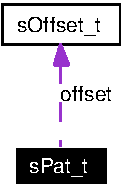
\includegraphics[width=46pt]{structsPat__t__coll__graph}
\end{center}
\end{figure}
\subsection*{Data Fields}
\begin{CompactItemize}
\item 
char $\ast$ \hyperlink{structsPat__t_o0}{string}
\item 
int \hyperlink{structsPat__t_o1}{length}
\item 
int \hyperlink{structsPat__t_o2}{support}
\item 
\hyperlink{structsOffset__t}{s\-Offset\_\-t} $\ast$ \hyperlink{structsPat__t_o3}{offset}
\end{CompactItemize}


\subsection*{Detailed Description}
This data structure is used to store the locations of all the instances of a particular word of length {\em length\/} in a set of sequences. This data structure is used principally by the string based version of Gemoda and is used to store words that are hashed before the comparison phase.



Definition at line 36 of file spat.h.

\subsection*{Field Documentation}
\hypertarget{structsPat__t_o1}{
\index{sPat_t@{s\-Pat\_\-t}!length@{length}}
\index{length@{length}!sPat_t@{s\-Pat\_\-t}}
\subsubsection[length]{\setlength{\rightskip}{0pt plus 5cm}int \hyperlink{structsPat__t_o1}{s\-Pat\_\-t::length}}}
\label{structsPat__t_o1}


The length of this word.

Definition at line 43 of file spat.h.

Referenced by count\-Words2(), and print\-SPats().\hypertarget{structsPat__t_o3}{
\index{sPat_t@{s\-Pat\_\-t}!offset@{offset}}
\index{offset@{offset}!sPat_t@{s\-Pat\_\-t}}
\subsubsection[offset]{\setlength{\rightskip}{0pt plus 5cm}\hyperlink{structsOffset__t}{s\-Offset\_\-t}$\ast$ \hyperlink{structsPat__t_o3}{s\-Pat\_\-t::offset}}}
\label{structsPat__t_o3}


An array of \hyperlink{structsOffset__t}{s\-Offset\_\-t} objects storing the loci, or offsets where this word occurs.

Definition at line 50 of file spat.h.

Referenced by count\-Words2(), destroy\-SPat\-A(), and main().\hypertarget{structsPat__t_o0}{
\index{sPat_t@{s\-Pat\_\-t}!string@{string}}
\index{string@{string}!sPat_t@{s\-Pat\_\-t}}
\subsubsection[string]{\setlength{\rightskip}{0pt plus 5cm}char$\ast$ \hyperlink{structsPat__t_o0}{s\-Pat\_\-t::string}}}
\label{structsPat__t_o0}


The pointer to the string for this word.

Definition at line 40 of file spat.h.

Referenced by count\-Words2().\hypertarget{structsPat__t_o2}{
\index{sPat_t@{s\-Pat\_\-t}!support@{support}}
\index{support@{support}!sPat_t@{s\-Pat\_\-t}}
\subsubsection[support]{\setlength{\rightskip}{0pt plus 5cm}int \hyperlink{structsPat__t_o2}{s\-Pat\_\-t::support}}}
\label{structsPat__t_o2}


The number of times this word occurs in the sequence set.

Definition at line 46 of file spat.h.

Referenced by count\-Words2().

The documentation for this struct was generated from the following file:\begin{CompactItemize}
\item 
\hyperlink{spat_8h}{spat.h}\end{CompactItemize}

\hypertarget{structsSize__t}{
\section{s\-Size\_\-t Struct Reference}
\label{structsSize__t}\index{sSize_t@{sSize\_\-t}}
}
\subsection*{Data Fields}
\begin{CompactItemize}
\item 
int \hyperlink{structsSize__t_o0}{start}
\item 
int \hyperlink{structsSize__t_o1}{stop}
\item 
int \hyperlink{structsSize__t_o2}{size}
\end{CompactItemize}


\subsection*{Detailed Description}




Definition at line 165 of file fasta\-Seq\-IO.c.

\subsection*{Field Documentation}
\hypertarget{structsSize__t_o2}{
\index{sSize_t@{s\-Size\_\-t}!size@{size}}
\index{size@{size}!sSize_t@{s\-Size\_\-t}}
\subsubsection[size]{\setlength{\rightskip}{0pt plus 5cm}int \hyperlink{structsSize__t_o2}{s\-Size\_\-t::size}}}
\label{structsSize__t_o2}




Definition at line 168 of file fasta\-Seq\-IO.c.

Referenced by Read\-FSeqs().\hypertarget{structsSize__t_o0}{
\index{sSize_t@{s\-Size\_\-t}!start@{start}}
\index{start@{start}!sSize_t@{s\-Size\_\-t}}
\subsubsection[start]{\setlength{\rightskip}{0pt plus 5cm}int \hyperlink{structsSize__t_o0}{s\-Size\_\-t::start}}}
\label{structsSize__t_o0}




Definition at line 166 of file fasta\-Seq\-IO.c.

Referenced by Read\-FSeqs().\hypertarget{structsSize__t_o1}{
\index{sSize_t@{s\-Size\_\-t}!stop@{stop}}
\index{stop@{stop}!sSize_t@{s\-Size\_\-t}}
\subsubsection[stop]{\setlength{\rightskip}{0pt plus 5cm}int \hyperlink{structsSize__t_o1}{s\-Size\_\-t::stop}}}
\label{structsSize__t_o1}




Definition at line 167 of file fasta\-Seq\-IO.c.

Referenced by Read\-FSeqs().

The documentation for this struct was generated from the following file:\begin{CompactItemize}
\item 
Fasta\-Seq\-IO/\hyperlink{fastaSeqIO_8c}{fasta\-Seq\-IO.c}\end{CompactItemize}

\chapter{gemoda File Documentation}
\hypertarget{align_8c}{
\section{align.c File Reference}
\label{align_8c}\index{align.c@{align.c}}
}
{\tt \#include $<$stdio.h$>$}\par
{\tt \#include $<$stdlib.h$>$}\par
{\tt \#include $<$string.h$>$}\par
{\tt \#include $<$errno.h$>$}\par
{\tt \#include \char`\"{}Fasta\-Seq\-IO/fasta\-Seq\-IO.h\char`\"{}}\par
{\tt \#include \char`\"{}spat.h\char`\"{}}\par
{\tt \#include \char`\"{}bit\-Set.h\char`\"{}}\par
{\tt \#include \char`\"{}matdata.h\char`\"{}}\par


Include dependency graph for align.c:\begin{figure}[H]
\begin{center}
\leavevmode
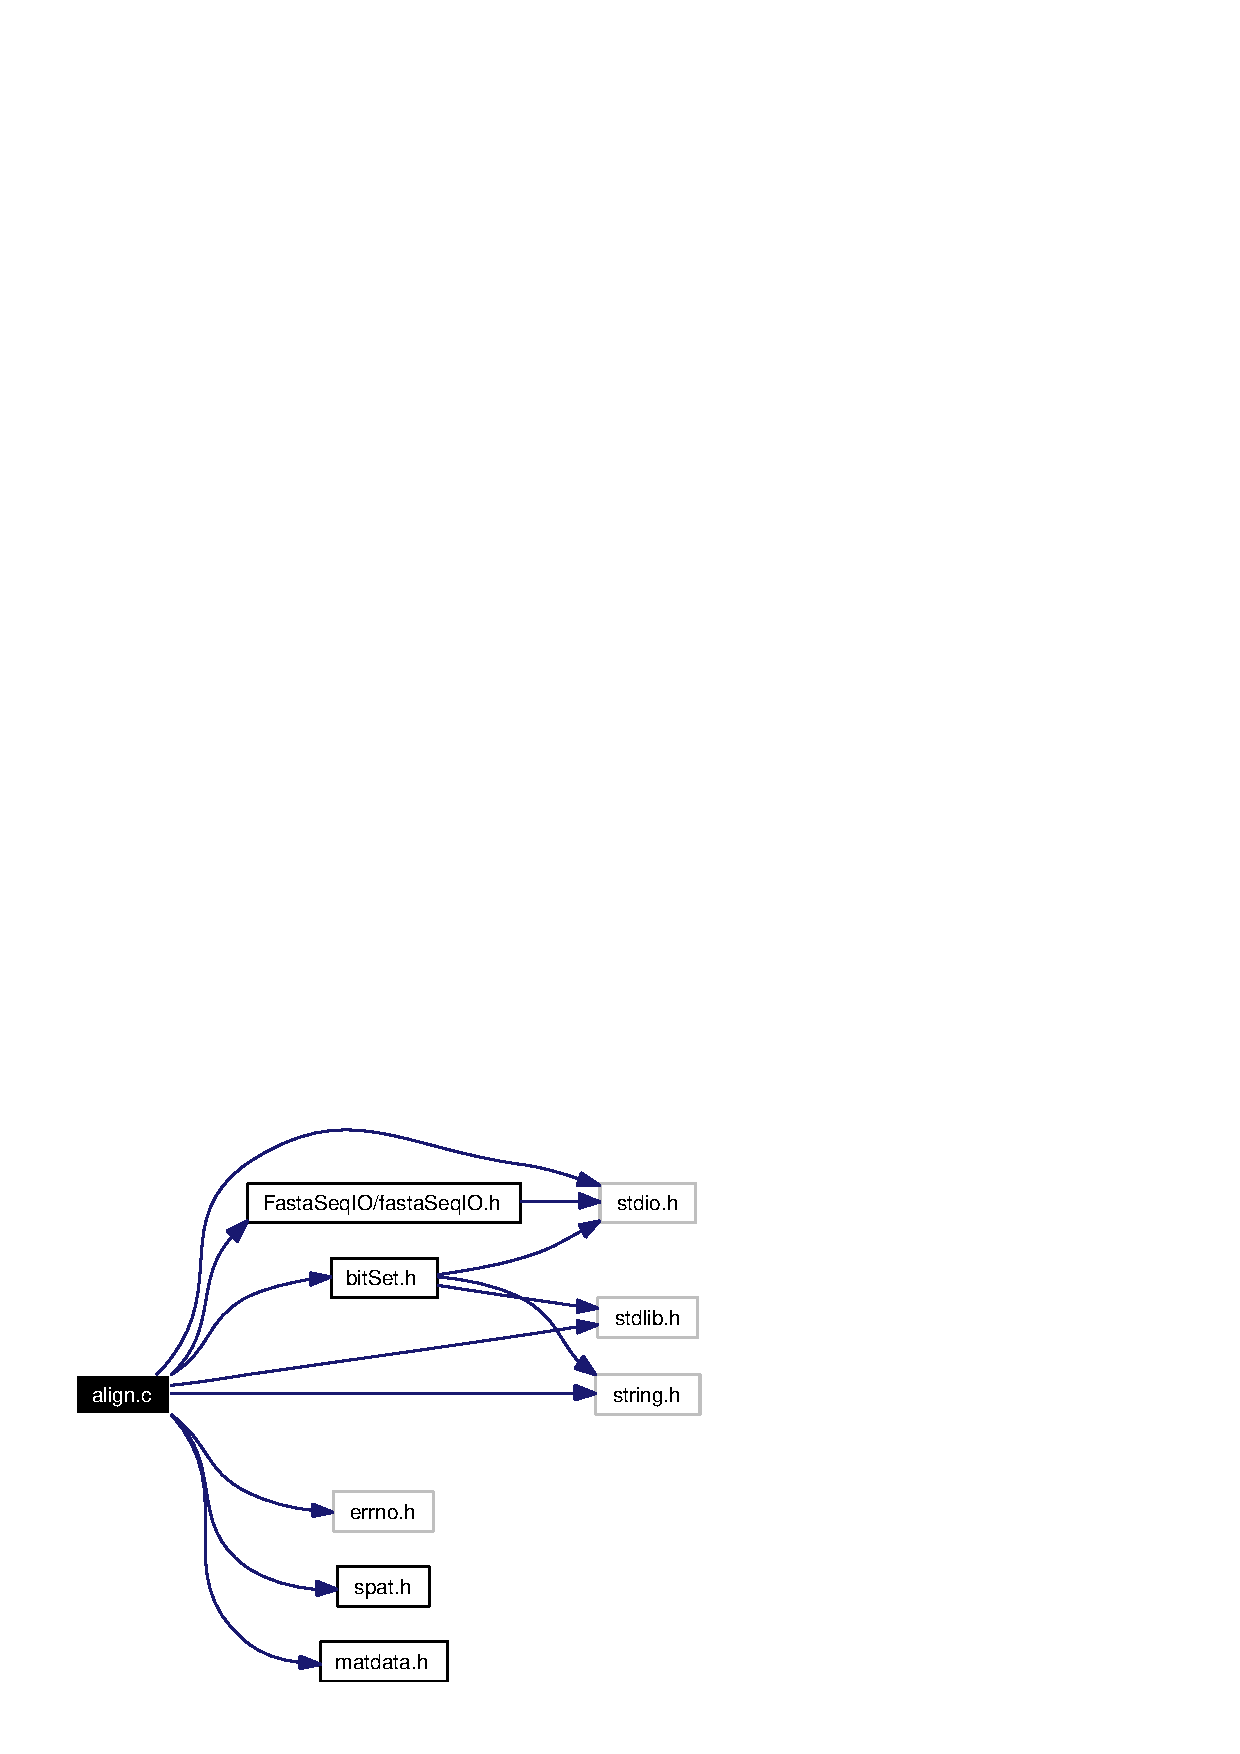
\includegraphics[width=168pt]{align_8c__incl}
\end{center}
\end{figure}
\subsection*{Defines}
\begin{CompactItemize}
\item 
\#define \hyperlink{align_8c_a0}{ALIGN\_\-ALPHABET}~256
\end{CompactItemize}
\subsection*{Functions}
\begin{CompactItemize}
\item 
int \hyperlink{align_8c_a2}{align\-Mat} (char $\ast$s1, char $\ast$s2, int L, int \hyperlink{matrixmap_8h_a1}{mat}\mbox{[}$\,$\mbox{]}\mbox{[}MATRIX\_\-SIZE\mbox{]})
\item 
\hyperlink{structbitGraph__t}{bit\-Graph\_\-t} $\ast$ \hyperlink{align_8c_a3}{align\-Words\-Mat\_\-bit} (\hyperlink{structsPat__t}{s\-Pat\_\-t} $\ast$words, int wc, int \hyperlink{matrixmap_8h_a1}{mat}\mbox{[}$\,$\mbox{]}\mbox{[}MATRIX\_\-SIZE\mbox{]}, int threshold)
\end{CompactItemize}
\subsection*{Variables}
\begin{CompactItemize}
\item 
const int \hyperlink{align_8c_a1}{aa\-Order} \mbox{[}$\,$\mbox{]}
\end{CompactItemize}


\subsection*{Detailed Description}
This file defines functions that are used to create a similarity graph, or adjacency matrix via the comparison of small windows within a set of sequences. This file is only used for string based sequences, and not real valued data. Usually, the adjacency matrix is created via a the alignment of the windows within the sequence set. Thus, the name of this file. However, other functions can certainly be defined for creating the adjacency matrix.

Definition in file \hyperlink{align_8c-source}{align.c}.

\subsection*{Define Documentation}
\hypertarget{align_8c_a0}{
\index{align.c@{align.c}!ALIGN_ALPHABET@{ALIGN\_\-ALPHABET}}
\index{ALIGN_ALPHABET@{ALIGN\_\-ALPHABET}!align.c@{align.c}}
\subsubsection[ALIGN\_\-ALPHABET]{\setlength{\rightskip}{0pt plus 5cm}\#define ALIGN\_\-ALPHABET~256}}
\label{align_8c_a0}




Definition at line 24 of file align.c.

\subsection*{Function Documentation}
\hypertarget{align_8c_a2}{
\index{align.c@{align.c}!alignMat@{alignMat}}
\index{alignMat@{alignMat}!align.c@{align.c}}
\subsubsection[alignMat]{\setlength{\rightskip}{0pt plus 5cm}int align\-Mat (char $\ast$ {\em s1}, char $\ast$ {\em s2}, int {\em L}, int {\em mat}\mbox{[}$\,$\mbox{]}\mbox{[}MATRIX\_\-SIZE\mbox{]})}}
\label{align_8c_a2}


This function takes as its arguments two pointers to strings, a length, and a scoring matrix. The function computes the score, or degree of similarity, between the two strings by comparing each character the in the strings from zero two L minus one. Each character receives a score that is looked up in the scoring matrix. This is most commonly used for amino acid sequences or DNA sequences; however, it is applicable to any series of characters. This function returns a single integer, which is the score between the two words.

Definition at line 44 of file align.c.

References aa\-Order, and mat.

Referenced by align\-Words\-Mat\_\-bit().

\scriptsize\begin{verbatim}45 {
46   int i;
47   int points = 0;
48   int x, y;
49   
50     // Go over each character in the L-length window
51     for (i = 0; i < L; i++)
52     {
53       
54     // The integer corresponding to the character in
55     // the first string, so that we can look it up 
56     // in one of our scoring matricies.
57     x = aaOrder[(int) s1[i]];
58       
59     // And for the second character
60     y = aaOrder[(int) s2[i]];
61       
62     // If the characters aren't going to be in the scoring
63     // matrix, they get a -1 value...which we'll give zero
64     // points to here.
65     if (x != -1 && y != -1)
66     {
67       
68         // Otherwise, they get a score that is looked up
69         // in the scoring matrix
70         points += mat[x][y];
71     }
72     }
73   return points;
74 }
\end{verbatim}
\normalsize 


\hypertarget{align_8c_a3}{
\index{align.c@{align.c}!alignWordsMat_bit@{alignWordsMat\_\-bit}}
\index{alignWordsMat_bit@{alignWordsMat\_\-bit}!align.c@{align.c}}
\subsubsection[alignWordsMat\_\-bit]{\setlength{\rightskip}{0pt plus 5cm}\hyperlink{structbitGraph__t}{bit\-Graph\_\-t}$\ast$ align\-Words\-Mat\_\-bit (\hyperlink{structsPat__t}{s\-Pat\_\-t} $\ast$ {\em words}, int {\em wc}, int {\em mat}\mbox{[}$\,$\mbox{]}\mbox{[}MATRIX\_\-SIZE\mbox{]}, int {\em threshold})}}
\label{align_8c_a3}


This uses the function above. Here, we have an array of words (\hyperlink{structsPat__t}{s\-Pat\_\-t} objects) and we compare (align) them all. If their score is above 'threshold' then we will set a bit to 'true' in a \hyperlink{structbitGraph__t}{bit\-Graph\_\-t} that we create. A \hyperlink{structbitGraph__t}{bit\-Graph\_\-t} is essentially an adjacency matrix, where each member of the matrix contains only a single bit: are the words equal, true or false? The function traverses the words by doing and all by all comparison; however, we only do the upper diagonal. The function makes use of align\-Mat and needs to be passed a scoring matrix that the user has chosen which is appropriate for the context of whatever data sent the user is looking at.

Definition at line 88 of file align.c.

References align\-Mat(), bit\-Graph\-Set\-True\-Sym(), mat, and new\-Bit\-Graph().

Referenced by main().

\scriptsize\begin{verbatim}90 {
91   bitGraph_t * sg = NULL;
92   int score;
93   int i, j;
94   
95     // Assign a new bitGraph_t object, with (wc x wc) possible
96     // true/false values
97     sg = newBitGraph (wc);
98   for (i = 0; i < wc; i++)
99     {
100       for (j = i; j < wc; j++)
101     {
102       
103         // Get the score for the alignment of word i and word j
104         score =
105         alignMat (words[i].string, words[j].string, words[i].length, mat);
106       
107         // If that score is greater than threshold, set
108         // a bit to 'true' in our bitGraph_t object
109         if (score >= threshold)
110         {
111           
112         // We use 'bitGraphSetTrueSym' because, if i=j,
113         // then j=i for most applications.  However, this
114         // can be relaxed for masochists.
115         bitGraphSetTrueSym (sg, i, j);
116         }
117     }
118     }
119   
120     // Return a pointer to this new bitGraph_t object
121     return sg;
122 }
\end{verbatim}

\normalsize 




\subsection*{Variable Documentation}
\hypertarget{align_8c_a1}{
\index{align.c@{align.c}!aaOrder@{aaOrder}}
\index{aaOrder@{aaOrder}!align.c@{align.c}}
\subsubsection[aaOrder]{\setlength{\rightskip}{0pt plus 5cm}const int \hyperlink{matrices_8h_a0}{aa\-Order}\mbox{[}$\,$\mbox{]}}}
\label{align_8c_a1}




Definition at line 32 of file matrices.h.

Referenced by align\-Mat().

\hypertarget{bitSet_8c}{
\section{bit\-Set.c File Reference}
\label{bitSet_8c}\index{bitSet.c@{bitSet.c}}
}
{\tt \#include \char`\"{}errno.h\char`\"{}}\par
{\tt \#include \char`\"{}bit\-Set.h\char`\"{}}\par


Include dependency graph for bit\-Set.c:\begin{figure}[H]
\begin{center}
\leavevmode
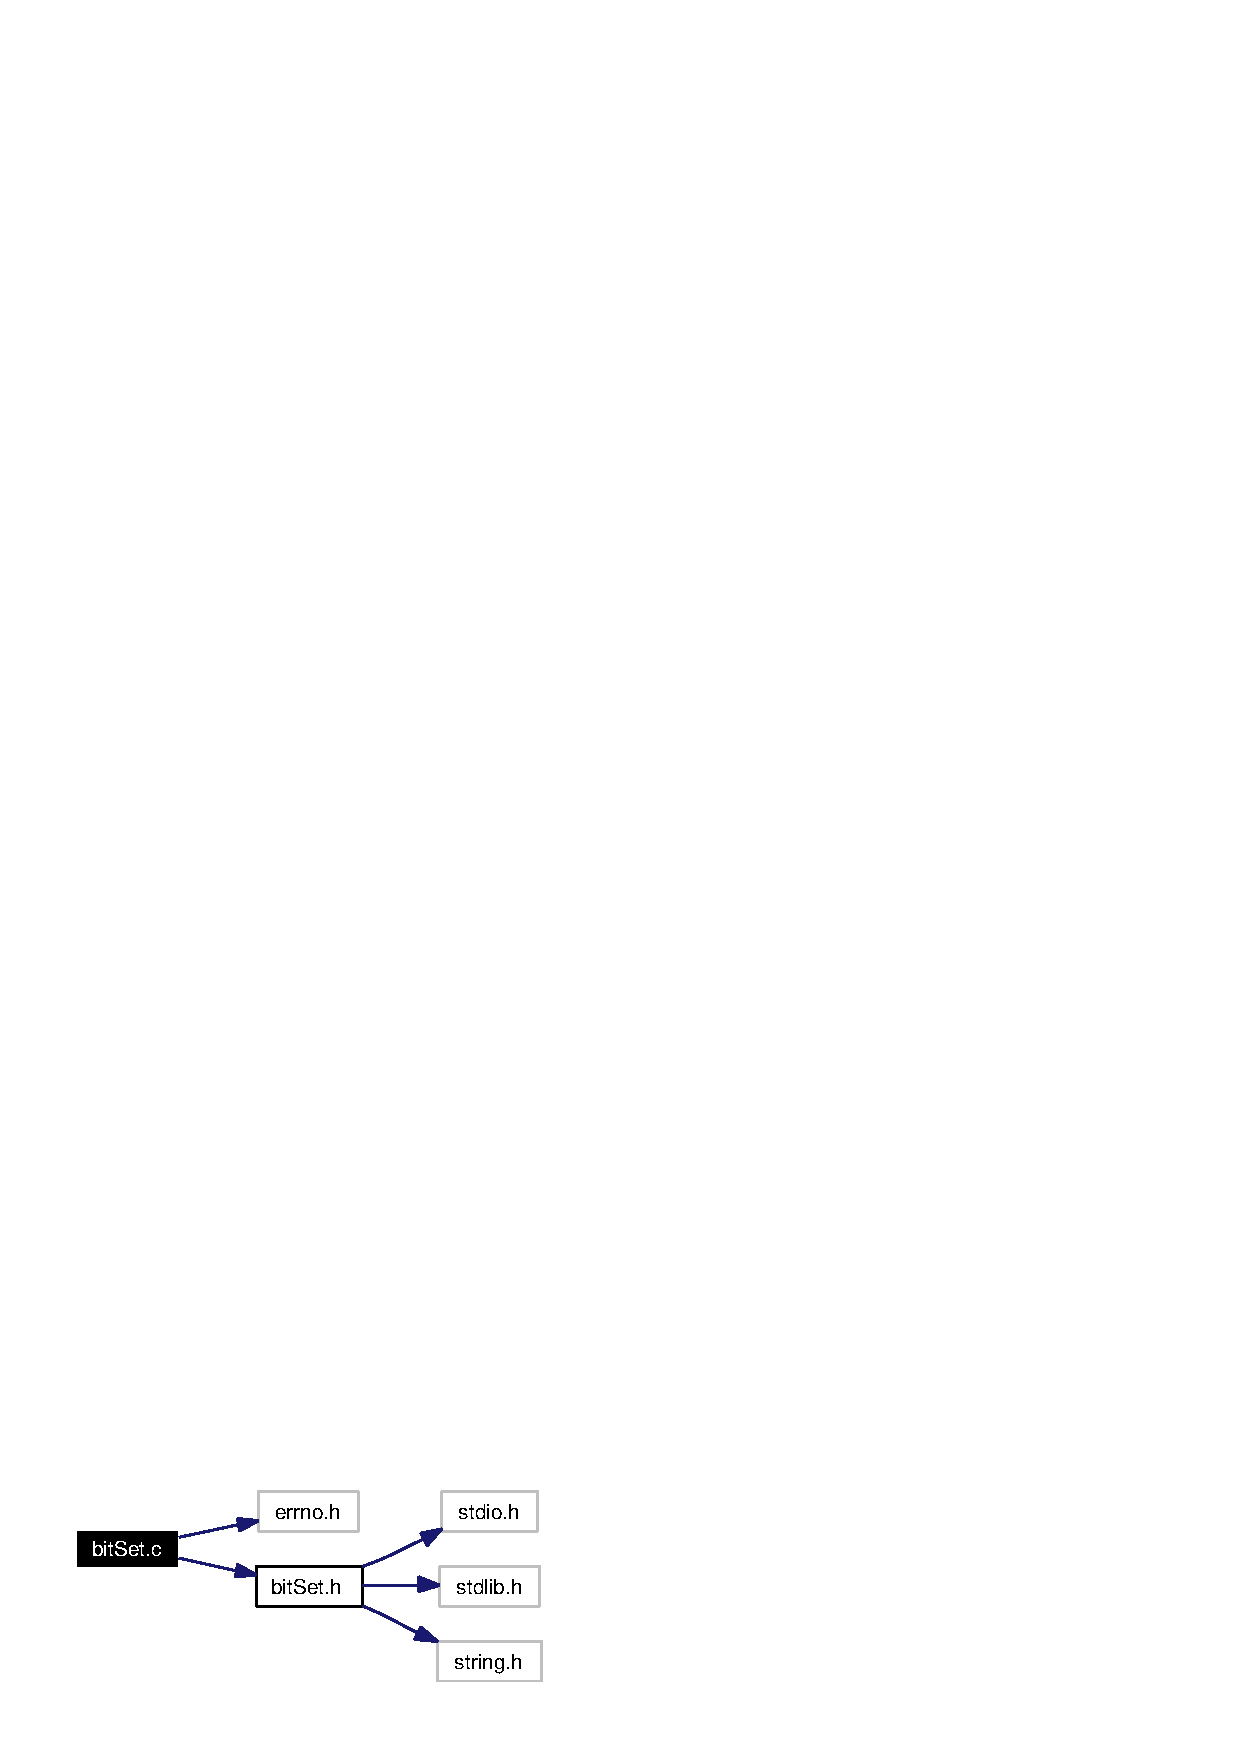
\includegraphics[width=130pt]{bitSet_8c__incl}
\end{center}
\end{figure}
\subsection*{Functions}
\begin{CompactItemize}
\item 
\hyperlink{bitSet_8h_a9}{bit\_\-t} $\ast$ \hyperlink{bitSet_8c_a1}{new\-Bit\-Array} (int bytes)
\item 
\hyperlink{structbitSet__t}{bit\-Set\_\-t} $\ast$ \hyperlink{bitSet_8c_a2}{new\-Bit\-Set} (int size)
\item 
int \hyperlink{bitSet_8c_a3}{set\-True} (\hyperlink{structbitSet__t}{bit\-Set\_\-t} $\ast$s1, int x)
\item 
int \hyperlink{bitSet_8c_a4}{set\-False} (\hyperlink{structbitSet__t}{bit\-Set\_\-t} $\ast$s1, int x)
\item 
int \hyperlink{bitSet_8c_a5}{flip\-Bits} (\hyperlink{structbitSet__t}{bit\-Set\_\-t} $\ast$s1)
\item 
int \hyperlink{bitSet_8c_a6}{fill\-Set} (\hyperlink{structbitSet__t}{bit\-Set\_\-t} $\ast$s1)
\item 
int \hyperlink{bitSet_8c_a7}{empty\-Set} (\hyperlink{structbitSet__t}{bit\-Set\_\-t} $\ast$s1)
\item 
int \hyperlink{bitSet_8c_a8}{check\-Bit} (\hyperlink{structbitSet__t}{bit\-Set\_\-t} $\ast$s1, int x)
\item 
int \hyperlink{bitSet_8c_a9}{delete\-Bit\-Set} (\hyperlink{structbitSet__t}{bit\-Set\_\-t} $\ast$s1)
\item 
int \hyperlink{bitSet_8c_a10}{bit\-Set\-Union} (\hyperlink{structbitSet__t}{bit\-Set\_\-t} $\ast$s1, \hyperlink{structbitSet__t}{bit\-Set\_\-t} $\ast$s2, \hyperlink{structbitSet__t}{bit\-Set\_\-t} $\ast$s3)
\item 
int \hyperlink{bitSet_8c_a11}{copy\-Set} (\hyperlink{structbitSet__t}{bit\-Set\_\-t} $\ast$s1, \hyperlink{structbitSet__t}{bit\-Set\_\-t} $\ast$s2)
\item 
int \hyperlink{bitSet_8c_a12}{copy\-Bit\-Graph} (\hyperlink{structbitGraph__t}{bit\-Graph\_\-t} $\ast$bg1, \hyperlink{structbitGraph__t}{bit\-Graph\_\-t} $\ast$bg2)
\item 
int \hyperlink{bitSet_8c_a13}{bit\-Set\-Difference} (\hyperlink{structbitSet__t}{bit\-Set\_\-t} $\ast$s1, \hyperlink{structbitSet__t}{bit\-Set\_\-t} $\ast$s2, \hyperlink{structbitSet__t}{bit\-Set\_\-t} $\ast$s3)
\item 
int \hyperlink{bitSet_8c_a14}{bit\-Set\-Sum} (\hyperlink{structbitSet__t}{bit\-Set\_\-t} $\ast$s1, \hyperlink{structbitSet__t}{bit\-Set\_\-t} $\ast$s2, \hyperlink{structbitSet__t}{bit\-Set\_\-t} $\ast$s3)
\item 
int \hyperlink{bitSet_8c_a15}{bit\-Set\-Intersection} (\hyperlink{structbitSet__t}{bit\-Set\_\-t} $\ast$s1, \hyperlink{structbitSet__t}{bit\-Set\_\-t} $\ast$s2, \hyperlink{structbitSet__t}{bit\-Set\_\-t} $\ast$s3)
\item 
int \hyperlink{bitSet_8c_a16}{bit\-Set3Way\-Intersection} (\hyperlink{structbitSet__t}{bit\-Set\_\-t} $\ast$s1, \hyperlink{structbitSet__t}{bit\-Set\_\-t} $\ast$s2, \hyperlink{structbitSet__t}{bit\-Set\_\-t} $\ast$s3, \hyperlink{structbitSet__t}{bit\-Set\_\-t} $\ast$s4)
\item 
int \hyperlink{bitSet_8c_a17}{bitcount32} (unsigned int n)
\item 
int \hyperlink{bitSet_8c_a18}{bitcount32\_\-precomp} (unsigned int n)
\item 
int \hyperlink{bitSet_8c_a19}{bitcount64} (unsigned int n)
\item 
int \hyperlink{bitSet_8c_a20}{count\-Set} (\hyperlink{structbitSet__t}{bit\-Set\_\-t} $\ast$s1)
\item 
int \hyperlink{bitSet_8c_a21}{next\-Bit\-Bit\-Set} (\hyperlink{structbitSet__t}{bit\-Set\_\-t} $\ast$s1, int start)
\item 
int \hyperlink{bitSet_8c_a22}{count\-Bit\-Graph\-Non\-Zero} (\hyperlink{structbitGraph__t}{bit\-Graph\_\-t} $\ast$bg)
\item 
int \hyperlink{bitSet_8c_a23}{print\-Bit\-Set} (\hyperlink{structbitSet__t}{bit\-Set\_\-t} $\ast$s1)
\item 
int \hyperlink{bitSet_8c_a24}{bit\-Graph\-Row\-Union} (\hyperlink{structbitGraph__t}{bit\-Graph\_\-t} $\ast$bg, int row1, int row2, \hyperlink{structbitSet__t}{bit\-Set\_\-t} $\ast$s1)
\item 
int \hyperlink{bitSet_8c_a25}{bit\-Graph\-Row\-Intersection} (\hyperlink{structbitGraph__t}{bit\-Graph\_\-t} $\ast$bg, int row1, int row2, \hyperlink{structbitSet__t}{bit\-Set\_\-t} $\ast$s1)
\item 
int \hyperlink{bitSet_8c_a26}{print\-Binary\-Bit\-Set} (\hyperlink{structbitSet__t}{bit\-Set\_\-t} $\ast$s1)
\item 
int \hyperlink{bitSet_8c_a27}{bit\-Graph\-Check\-Bit} (\hyperlink{structbitGraph__t}{bit\-Graph\_\-t} $\ast$bg, int x, int y)
\item 
int \hyperlink{bitSet_8c_a28}{bit\-Graph\-Set\-True} (\hyperlink{structbitGraph__t}{bit\-Graph\_\-t} $\ast$bg, int x, int y)
\item 
int \hyperlink{bitSet_8c_a29}{bit\-Graph\-Set\-False} (\hyperlink{structbitGraph__t}{bit\-Graph\_\-t} $\ast$bg, int x, int y)
\item 
int \hyperlink{bitSet_8c_a30}{bit\-Graph\-Set\-False\-Sym} (\hyperlink{structbitGraph__t}{bit\-Graph\_\-t} $\ast$bg, int x, int y)
\item 
int \hyperlink{bitSet_8c_a31}{bit\-Graph\-Set\-True\-Sym} (\hyperlink{structbitGraph__t}{bit\-Graph\_\-t} $\ast$bg, int x, int y)
\item 
int \hyperlink{bitSet_8c_a32}{bit\-Graph\-Set\-True\-Diagonal} (\hyperlink{structbitGraph__t}{bit\-Graph\_\-t} $\ast$bg)
\item 
int \hyperlink{bitSet_8c_a33}{bit\-Graph\-Set\-False\-Diagonal} (\hyperlink{structbitGraph__t}{bit\-Graph\_\-t} $\ast$bg)
\item 
int \hyperlink{bitSet_8c_a34}{print\-Bit\-Graph} (\hyperlink{structbitGraph__t}{bit\-Graph\_\-t} $\ast$bg)
\item 
int \hyperlink{bitSet_8c_a35}{mask\-Bit\-Graph} (\hyperlink{structbitGraph__t}{bit\-Graph\_\-t} $\ast$bg1, \hyperlink{structbitSet__t}{bit\-Set\_\-t} $\ast$bs)
\item 
int \hyperlink{bitSet_8c_a36}{fill\-Bit\-Graph} (\hyperlink{structbitGraph__t}{bit\-Graph\_\-t} $\ast$bg1)
\item 
int \hyperlink{bitSet_8c_a37}{empty\-Bit\-Graph} (\hyperlink{structbitGraph__t}{bit\-Graph\_\-t} $\ast$bg1)
\item 
\hyperlink{structbitGraph__t}{bit\-Graph\_\-t} $\ast$ \hyperlink{bitSet_8c_a38}{new\-Bit\-Graph} (int size)
\item 
int \hyperlink{bitSet_8c_a39}{empty\-Bit\-Graph\-Row} (\hyperlink{structbitGraph__t}{bit\-Graph\_\-t} $\ast$bg, int row)
\item 
int \hyperlink{bitSet_8c_a40}{delete\-Bit\-Graph} (\hyperlink{structbitGraph__t}{bit\-Graph\_\-t} $\ast$bg)
\end{CompactItemize}


\subsection*{Detailed Description}
This file defines functions for handling bit sets and bit graphs.

Definition in file \hyperlink{bitSet_8c-source}{bit\-Set.c}.

\subsection*{Function Documentation}
\hypertarget{bitSet_8c_a17}{
\index{bitSet.c@{bit\-Set.c}!bitcount32@{bitcount32}}
\index{bitcount32@{bitcount32}!bitSet.c@{bit\-Set.c}}
\subsubsection[bitcount32]{\setlength{\rightskip}{0pt plus 5cm}int bitcount32 (unsigned int {\em n})}}
\label{bitSet_8c_a17}


Attempt at a fast way of counting how many true values are in a given \hyperlink{structbitSet__t}{bit\-Set\_\-t}. Currently deprecated, using precompiled version instead.

Definition at line 351 of file bit\-Set.c.

\scriptsize\begin{verbatim}352 {
353   /*
354      works for 32-bit numbers only 
355    */
356   /*
357      fix last line for 64-bit numbers 
358    */
359 
360   register unsigned int tmp;
361 
362   tmp = n - ((n >> 1) & 033333333333) - ((n >> 2) & 011111111111);
363   return ((tmp + (tmp >> 3)) & 030707070707) % 63;
364 }
\end{verbatim}
\normalsize 


\hypertarget{bitSet_8c_a18}{
\index{bitSet.c@{bit\-Set.c}!bitcount32_precomp@{bitcount32\_\-precomp}}
\index{bitcount32_precomp@{bitcount32\_\-precomp}!bitSet.c@{bit\-Set.c}}
\subsubsection[bitcount32\_\-precomp]{\setlength{\rightskip}{0pt plus 5cm}int bitcount32\_\-precomp (unsigned int {\em n})}}
\label{bitSet_8c_a18}


Uses bits\_\-in\_\-char data structure to determine the number of true bits in a 32-bit int in an efficient manner. Input: 32-bit int (equal to one slot in the bit\-Set). Output: number of true bits in the input integer.

Definition at line 396 of file bit\-Set.c.

Referenced by count\-Set().

\scriptsize\begin{verbatim}397 {
398   // works only for 32-bit ints
399 
400   return bits_in_char[n & 0xffu]
401     + bits_in_char[(n >> 8) & 0xffu]
402     + bits_in_char[(n >> 16) & 0xffu] + bits_in_char[(n >> 24) & 0xffu];
403 }
\end{verbatim}
\normalsize 


\hypertarget{bitSet_8c_a19}{
\index{bitSet.c@{bit\-Set.c}!bitcount64@{bitcount64}}
\index{bitcount64@{bitcount64}!bitSet.c@{bit\-Set.c}}
\subsubsection[bitcount64]{\setlength{\rightskip}{0pt plus 5cm}int bitcount64 (unsigned int {\em n})}}
\label{bitSet_8c_a19}


Currently there is no support for 64-bit architectures.

Definition at line 420 of file bit\-Set.c.

\scriptsize\begin{verbatim}421 {
422   n = PCCOUNT (n, 0);
423   n = PCCOUNT (n, 1);
424   n = PCCOUNT (n, 2);
425   n = PCCOUNT (n, 3);
426   n = PCCOUNT (n, 4);
427   n = PCCOUNT (n, 5);       // for 64-bit integers 
428   return n;
429 }
\end{verbatim}
\normalsize 


\hypertarget{bitSet_8c_a27}{
\index{bitSet.c@{bit\-Set.c}!bitGraphCheckBit@{bitGraphCheckBit}}
\index{bitGraphCheckBit@{bitGraphCheckBit}!bitSet.c@{bit\-Set.c}}
\subsubsection[bitGraphCheckBit]{\setlength{\rightskip}{0pt plus 5cm}int bit\-Graph\-Check\-Bit (\hyperlink{structbitGraph__t}{bit\-Graph\_\-t} $\ast$ {\em bg}, int {\em x}, int {\em y})}}
\label{bitSet_8c_a27}


Checks the value of a bit in a \hyperlink{structbitGraph__t}{bit\-Graph\_\-t} object. Input: a \hyperlink{structbitGraph__t}{bit\-Graph\_\-t} object, the index of the row of the \hyperlink{structbitGraph__t}{bit\-Graph\_\-t} with the bit to be checked, the index of the bit in that row that is to be checked. Output: the value of the bit in the bit\-Graph being checked.

Definition at line 628 of file bit\-Set.c.

References check\-Bit(), and bit\-Graph\_\-t::graph.

Referenced by main(), and measure\-Diagonal().

\scriptsize\begin{verbatim}629 {
630   return checkBit (bg->graph[x], y);
631 }
\end{verbatim}
\normalsize 


\hypertarget{bitSet_8c_a25}{
\index{bitSet.c@{bit\-Set.c}!bitGraphRowIntersection@{bitGraphRowIntersection}}
\index{bitGraphRowIntersection@{bitGraphRowIntersection}!bitSet.c@{bit\-Set.c}}
\subsubsection[bitGraphRowIntersection]{\setlength{\rightskip}{0pt plus 5cm}int bit\-Graph\-Row\-Intersection (\hyperlink{structbitGraph__t}{bit\-Graph\_\-t} $\ast$ {\em bg}, int {\em row1}, int {\em row2}, \hyperlink{structbitSet__t}{bit\-Set\_\-t} $\ast$ {\em s1})}}
\label{bitSet_8c_a25}


Finds the intersection of two rows (bit\-Sets) within a \hyperlink{structbitGraph__t}{bit\-Graph\_\-t} object. Input: a \hyperlink{structbitGraph__t}{bit\-Graph\_\-t} object, first row to be compared, second row to be compared, and a \hyperlink{structbitSet__t}{bit\-Set\_\-t} to store the intersection results. Output: integer success value of 0 (and an altered destination \hyperlink{structbitSet__t}{bit\-Set\_\-t} object with a true value wherever both source bit\-Sets had a true value).

Definition at line 598 of file bit\-Set.c.

References bit\-Set\-Intersection(), and bit\-Graph\_\-t::graph.

Referenced by get\-Stat\-Mat(), and old\-Get\-Stat\-Mat().

\scriptsize\begin{verbatim}599 {
600   bitSetIntersection (bg->graph[row1], bg->graph[row2], s1);
601   return 0;
602 }
\end{verbatim}
\normalsize 


\hypertarget{bitSet_8c_a24}{
\index{bitSet.c@{bit\-Set.c}!bitGraphRowUnion@{bitGraphRowUnion}}
\index{bitGraphRowUnion@{bitGraphRowUnion}!bitSet.c@{bit\-Set.c}}
\subsubsection[bitGraphRowUnion]{\setlength{\rightskip}{0pt plus 5cm}int bit\-Graph\-Row\-Union (\hyperlink{structbitGraph__t}{bit\-Graph\_\-t} $\ast$ {\em bg}, int {\em row1}, int {\em row2}, \hyperlink{structbitSet__t}{bit\-Set\_\-t} $\ast$ {\em s1})}}
\label{bitSet_8c_a24}


Finds the union of two rows (bit\-Sets) within a bit\-Graph Input: a \hyperlink{structbitGraph__t}{bit\-Graph\_\-t} object, first row to be compared, second row to be compared, and a \hyperlink{structbitSet__t}{bit\-Set\_\-t} to store the union results. Output: integer success value of 0 (and an altered destination \hyperlink{structbitSet__t}{bit\-Set\_\-t} object with a true value wherever one or both source bit\-Sets had a true value).

Definition at line 584 of file bit\-Set.c.

References bit\-Set\-Union(), and bit\-Graph\_\-t::graph.

\scriptsize\begin{verbatim}585 {
586   bitSetUnion (bg->graph[row1], bg->graph[row2], s1);
587   return 0;
588 }
\end{verbatim}
\normalsize 


\hypertarget{bitSet_8c_a29}{
\index{bitSet.c@{bit\-Set.c}!bitGraphSetFalse@{bitGraphSetFalse}}
\index{bitGraphSetFalse@{bitGraphSetFalse}!bitSet.c@{bit\-Set.c}}
\subsubsection[bitGraphSetFalse]{\setlength{\rightskip}{0pt plus 5cm}int bit\-Graph\-Set\-False (\hyperlink{structbitGraph__t}{bit\-Graph\_\-t} $\ast$ {\em bg}, int {\em x}, int {\em y})}}
\label{bitSet_8c_a29}


Sets a specific bit in a bit\-Graph false. Input: a \hyperlink{structbitGraph__t}{bit\-Graph\_\-t} object, the index of the row of the \hyperlink{structbitGraph__t}{bit\-Graph\_\-t} with the bit be set, the index of the bit in that row that is to be set. Output: integer success value of 0 (and an altered \hyperlink{structbitGraph__t}{bit\-Graph\_\-t} object).

Definition at line 654 of file bit\-Set.c.

References bit\-Graph\_\-t::graph, and set\-False().

\scriptsize\begin{verbatim}655 {
656   setFalse (bg->graph[x], y);
657   return 0;
658 }
\end{verbatim}
\normalsize 


\hypertarget{bitSet_8c_a33}{
\index{bitSet.c@{bit\-Set.c}!bitGraphSetFalseDiagonal@{bitGraphSetFalseDiagonal}}
\index{bitGraphSetFalseDiagonal@{bitGraphSetFalseDiagonal}!bitSet.c@{bit\-Set.c}}
\subsubsection[bitGraphSetFalseDiagonal]{\setlength{\rightskip}{0pt plus 5cm}int bit\-Graph\-Set\-False\-Diagonal (\hyperlink{structbitGraph__t}{bit\-Graph\_\-t} $\ast$ {\em bg})}}
\label{bitSet_8c_a33}


Sets the main diagonal of a bit\-Graph false. Input: a \hyperlink{structbitGraph__t}{bit\-Graph\_\-t} object. Output: integer success value of 0 (and an altered \hyperlink{structbitGraph__t}{bit\-Graph\_\-t} object).

Definition at line 714 of file bit\-Set.c.

References bit\-Graph\_\-t::graph, and set\-False().

Referenced by convolve().

\scriptsize\begin{verbatim}715 {
716   int i;
717   for (i = 0; i < bg->size; i++)
718     {
719       setFalse (bg->graph[i], i);
720     }
721   return 0;
722 }
\end{verbatim}
\normalsize 


\hypertarget{bitSet_8c_a30}{
\index{bitSet.c@{bit\-Set.c}!bitGraphSetFalseSym@{bitGraphSetFalseSym}}
\index{bitGraphSetFalseSym@{bitGraphSetFalseSym}!bitSet.c@{bit\-Set.c}}
\subsubsection[bitGraphSetFalseSym]{\setlength{\rightskip}{0pt plus 5cm}int bit\-Graph\-Set\-False\-Sym (\hyperlink{structbitGraph__t}{bit\-Graph\_\-t} $\ast$ {\em bg}, int {\em x}, int {\em y})}}
\label{bitSet_8c_a30}


Sets a specific bit and its symmetric opposite in a bit\-Graph false. For instance, given that we wanted to set the 3rd bit in the 5th row false, this would also set the 5th bit in the 3rd row. Input: a \hyperlink{structbitGraph__t}{bit\-Graph\_\-t} object, the index of the row of the bit\-Graph with the bit be set, the index of the bit in that row that is to be set. Output: integer success value of 0 (and an altered \hyperlink{structbitGraph__t}{bit\-Graph\_\-t} object).

Definition at line 669 of file bit\-Set.c.

References bit\-Graph\_\-t::graph, and set\-False().

\scriptsize\begin{verbatim}670 {
671   setFalse (bg->graph[x], y);
672   setFalse (bg->graph[y], x);
673   return 0;
674 }
\end{verbatim}
\normalsize 


\hypertarget{bitSet_8c_a28}{
\index{bitSet.c@{bit\-Set.c}!bitGraphSetTrue@{bitGraphSetTrue}}
\index{bitGraphSetTrue@{bitGraphSetTrue}!bitSet.c@{bit\-Set.c}}
\subsubsection[bitGraphSetTrue]{\setlength{\rightskip}{0pt plus 5cm}int bit\-Graph\-Set\-True (\hyperlink{structbitGraph__t}{bit\-Graph\_\-t} $\ast$ {\em bg}, int {\em x}, int {\em y})}}
\label{bitSet_8c_a28}


Sets a specific bit in a bit\-Graph true. Input: a \hyperlink{structbitGraph__t}{bit\-Graph\_\-t} object, the index of the row of the \hyperlink{structbitGraph__t}{bit\-Graph\_\-t} with the bit be set, the index of the bit in that row that is to be set. Output: integer success value of 0 (and an altered \hyperlink{structbitGraph__t}{bit\-Graph\_\-t} object).

Definition at line 641 of file bit\-Set.c.

References bit\-Graph\_\-t::graph, and set\-True().

\scriptsize\begin{verbatim}642 {
643   setTrue (bg->graph[x], y);
644   return 0;
645 }
\end{verbatim}
\normalsize 


\hypertarget{bitSet_8c_a32}{
\index{bitSet.c@{bit\-Set.c}!bitGraphSetTrueDiagonal@{bitGraphSetTrueDiagonal}}
\index{bitGraphSetTrueDiagonal@{bitGraphSetTrueDiagonal}!bitSet.c@{bit\-Set.c}}
\subsubsection[bitGraphSetTrueDiagonal]{\setlength{\rightskip}{0pt plus 5cm}int bit\-Graph\-Set\-True\-Diagonal (\hyperlink{structbitGraph__t}{bit\-Graph\_\-t} $\ast$ {\em bg})}}
\label{bitSet_8c_a32}


Sets the main diagonal of a bit\-Graph true. Input: a \hyperlink{structbitGraph__t}{bit\-Graph\_\-t} object. Output: integer success value of 0 (and an altered \hyperlink{structbitGraph__t}{bit\-Graph\_\-t} object).

Definition at line 698 of file bit\-Set.c.

References bit\-Graph\_\-t::graph, and set\-True().

\scriptsize\begin{verbatim}699 {
700   int i;
701   for (i = 0; i < bg->size; i++)
702     {
703       setTrue (bg->graph[i], i);
704     }
705   return 0;
706 }
\end{verbatim}
\normalsize 


\hypertarget{bitSet_8c_a31}{
\index{bitSet.c@{bit\-Set.c}!bitGraphSetTrueSym@{bitGraphSetTrueSym}}
\index{bitGraphSetTrueSym@{bitGraphSetTrueSym}!bitSet.c@{bit\-Set.c}}
\subsubsection[bitGraphSetTrueSym]{\setlength{\rightskip}{0pt plus 5cm}int bit\-Graph\-Set\-True\-Sym (\hyperlink{structbitGraph__t}{bit\-Graph\_\-t} $\ast$ {\em bg}, int {\em x}, int {\em y})}}
\label{bitSet_8c_a31}


Sets a specific bit and its symmetric opposite in a bit\-Graph true. For instance, given that we wanted to set the 3rd bit in the 5th row true, this would also set the 5th bit in the 3rd row. Input: a bit\-Graph, the index of the row of the bit\-Graph with the bit be set, the index of the bit in that row that is to be set. Output: integer success value of 0 (and an altered \hyperlink{structbitGraph__t}{bit\-Graph\_\-t} object).

Definition at line 685 of file bit\-Set.c.

References bit\-Graph\_\-t::graph, and set\-True().

Referenced by align\-Words\-Mat\_\-bit(), main(), and real\-Comparison().

\scriptsize\begin{verbatim}686 {
687   setTrue (bg->graph[x], y);
688   setTrue (bg->graph[y], x);
689   return 0;
690 }
\end{verbatim}
\normalsize 


\hypertarget{bitSet_8c_a16}{
\index{bitSet.c@{bit\-Set.c}!bitSet3WayIntersection@{bitSet3WayIntersection}}
\index{bitSet3WayIntersection@{bitSet3WayIntersection}!bitSet.c@{bit\-Set.c}}
\subsubsection[bitSet3WayIntersection]{\setlength{\rightskip}{0pt plus 5cm}int bit\-Set3Way\-Intersection (\hyperlink{structbitSet__t}{bit\-Set\_\-t} $\ast$ {\em s1}, \hyperlink{structbitSet__t}{bit\-Set\_\-t} $\ast$ {\em s2}, \hyperlink{structbitSet__t}{bit\-Set\_\-t} $\ast$ {\em s3}, \hyperlink{structbitSet__t}{bit\-Set\_\-t} $\ast$ {\em s4})}}
\label{bitSet_8c_a16}


Finds the intersection of 3 bit\-Sets. Input: First bit\-Set to be intersected, second bitset to be intersected. third bit\-Set to be intersected, a bit\-Set to store the result of the intersection. Output: Integer success value of 0 (and an altered destination \hyperlink{structbitSet__t}{bit\-Set\_\-t} object with a true where all three source bit\-Sets had a true.)

Definition at line 327 of file bit\-Set.c.

References BSINTERSECTION, bit\-Set\_\-t::slots, and bit\-Set\_\-t::tf.

\scriptsize\begin{verbatim}329 {
330   int i;
331   if ((s1->slots != s2->slots) || (s1->slots != s3->slots)
332       || (s1->slots != s4->slots))
333     {
334       fprintf (stderr, "Sets aren't same size!\n");
335       fflush (stderr);
336       exit (0);
337     }
338   for (i = 0; i < s1->slots; i++)
339     {
340       s4->tf[i] = BSINTERSECTION (s1->tf[i], s2->tf[i]);
341       s4->tf[i] = BSINTERSECTION (s3->tf[i], s4->tf[i]);
342     }
343   return 0;
344 }
\end{verbatim}
\normalsize 


\hypertarget{bitSet_8c_a13}{
\index{bitSet.c@{bit\-Set.c}!bitSetDifference@{bitSetDifference}}
\index{bitSetDifference@{bitSetDifference}!bitSet.c@{bit\-Set.c}}
\subsubsection[bitSetDifference]{\setlength{\rightskip}{0pt plus 5cm}int bit\-Set\-Difference (\hyperlink{structbitSet__t}{bit\-Set\_\-t} $\ast$ {\em s1}, \hyperlink{structbitSet__t}{bit\-Set\_\-t} $\ast$ {\em s2}, \hyperlink{structbitSet__t}{bit\-Set\_\-t} $\ast$ {\em s3})}}
\label{bitSet_8c_a13}


Locates all differences between two bit\-Sets. The result bit\-Set contains a true at a given bit if the two source bit\-Sets differ at that bit. Input: first bit set to be compared, second bit set to be compared. third bit set to store the results Output: integer success value of 0 (and an altered destination \hyperlink{structbitSet__t}{bit\-Set\_\-t} object with a true where the two source bit sets differed).

Definition at line 254 of file bit\-Set.c.

References bit\-Set\_\-t::slots, and bit\-Set\_\-t::tf.

\scriptsize\begin{verbatim}255 {
256   int i;
257   if ((s1->slots != s2->slots) || (s1->slots != s3->slots))
258     {
259       fprintf (stderr, "Sets aren't same size!\n");
260       fflush (stderr);
261       exit (0);
262     }
263   for (i = 0; i < s1->slots; i++)
264     {
265       s3->tf[i] = (s1->tf[i] & (~s2->tf[i]));
266     }
267   return 0;
268 }
\end{verbatim}
\normalsize 


\hypertarget{bitSet_8c_a15}{
\index{bitSet.c@{bit\-Set.c}!bitSetIntersection@{bitSetIntersection}}
\index{bitSetIntersection@{bitSetIntersection}!bitSet.c@{bit\-Set.c}}
\subsubsection[bitSetIntersection]{\setlength{\rightskip}{0pt plus 5cm}int bit\-Set\-Intersection (\hyperlink{structbitSet__t}{bit\-Set\_\-t} $\ast$ {\em s1}, \hyperlink{structbitSet__t}{bit\-Set\_\-t} $\ast$ {\em s2}, \hyperlink{structbitSet__t}{bit\-Set\_\-t} $\ast$ {\em s3})}}
\label{bitSet_8c_a15}


Finds the intersection of two bitsets. Input: First bit\-Set to be intersected, second bit\-Set to be intersected. a bit\-Set to store the result of the intersection. Output: Integer success value of 0 (and an altered destination \hyperlink{structbitSet__t}{bit\-Set\_\-t} object. with a true where both source bit\-Sets had a true).

Definition at line 299 of file bit\-Set.c.

References BSINTERSECTION, bit\-Set\_\-t::slots, and bit\-Set\_\-t::tf.

Referenced by bit\-Graph\-Row\-Intersection(), find\-Cliques(), and mask\-Bit\-Graph().

\scriptsize\begin{verbatim}300 {
301   int i;
302   if ((s1->slots != s2->slots) || (s1->slots != s3->slots))
303     {
304       fprintf (stderr, "Sets aren't same size!\n");
305       fprintf (stderr, "set 1 slots = %d\n", s1->slots);
306       fprintf (stderr, "set 2 slots = %d\n", s2->slots);
307       fprintf (stderr, "set 3 slots = %d\n", s3->slots);
308       fflush (stderr);
309       exit (0);
310     }
311   for (i = 0; i < s1->slots; i++)
312     {
313       s3->tf[i] = BSINTERSECTION (s1->tf[i], s2->tf[i]);
314     }
315   return 0;
316 }
\end{verbatim}
\normalsize 


\hypertarget{bitSet_8c_a14}{
\index{bitSet.c@{bit\-Set.c}!bitSetSum@{bitSetSum}}
\index{bitSetSum@{bitSetSum}!bitSet.c@{bit\-Set.c}}
\subsubsection[bitSetSum]{\setlength{\rightskip}{0pt plus 5cm}int bit\-Set\-Sum (\hyperlink{structbitSet__t}{bit\-Set\_\-t} $\ast$ {\em s1}, \hyperlink{structbitSet__t}{bit\-Set\_\-t} $\ast$ {\em s2}, \hyperlink{structbitSet__t}{bit\-Set\_\-t} $\ast$ {\em s3})}}
\label{bitSet_8c_a14}


Adds two \hyperlink{structbitSet__t}{bit\-Set\_\-t} objects together. Currently unknown functionality, not used in existing code.

Definition at line 275 of file bit\-Set.c.

References bit\-Set\_\-t::slots, and bit\-Set\_\-t::tf.

\scriptsize\begin{verbatim}276 {
277   int i;
278   if ((s1->slots != s2->slots) || (s1->slots != s3->slots))
279     {
280       fprintf (stderr, "Sets aren't same size!\n");
281       fflush (stderr);
282       exit (0);
283     }
284   for (i = 0; i < s1->slots; i++)
285     {
286       s3->tf[i] = (s1->tf[i] + s2->tf[i]);
287     }
288   return 0;
289 }
\end{verbatim}
\normalsize 


\hypertarget{bitSet_8c_a10}{
\index{bitSet.c@{bit\-Set.c}!bitSetUnion@{bitSetUnion}}
\index{bitSetUnion@{bitSetUnion}!bitSet.c@{bit\-Set.c}}
\subsubsection[bitSetUnion]{\setlength{\rightskip}{0pt plus 5cm}int bit\-Set\-Union (\hyperlink{structbitSet__t}{bit\-Set\_\-t} $\ast$ {\em s1}, \hyperlink{structbitSet__t}{bit\-Set\_\-t} $\ast$ {\em s2}, \hyperlink{structbitSet__t}{bit\-Set\_\-t} $\ast$ {\em s3})}}
\label{bitSet_8c_a10}


Finds the union of two bit\-Sets Input: first bit set for the union, second bit set for the union. a bit set in which to store the results Output: an integer success value of 0 (and an altered third \hyperlink{structbitSet__t}{bit\-Set\_\-t} with the results of the union.

Definition at line 182 of file bit\-Set.c.

References BSUNION, bit\-Set\_\-t::slots, and bit\-Set\_\-t::tf.

Referenced by bit\-Graph\-Row\-Union(), and single\-Linkage().

\scriptsize\begin{verbatim}183 {
184   int i;
185   if ((s1->slots != s2->slots) || (s1->slots != s3->slots))
186     {
187       fprintf (stderr, "Sets aren't same size!\n");
188       fflush (stderr);
189       exit (0);
190     }
191   for (i = 0; i < s1->slots; i++)
192     {
193       s3->tf[i] = BSUNION (s1->tf[i], s2->tf[i]);
194     }
195   return 0;
196 }
\end{verbatim}
\normalsize 


\hypertarget{bitSet_8c_a8}{
\index{bitSet.c@{bit\-Set.c}!checkBit@{checkBit}}
\index{checkBit@{checkBit}!bitSet.c@{bit\-Set.c}}
\subsubsection[checkBit]{\setlength{\rightskip}{0pt plus 5cm}int check\-Bit (\hyperlink{structbitSet__t}{bit\-Set\_\-t} $\ast$ {\em s1}, int {\em x})}}
\label{bitSet_8c_a8}


Finds the value of a specific bit in a bit\-Set. Input: a bit\-Set, the number of the bit being queried. Output: the value of the bit being queried (1 or 0).

Definition at line 148 of file bit\-Set.c.

References BSTEST, and bit\-Set\_\-t::tf.

Referenced by bit\-Graph\-Check\-Bit(), find\-Cliques(), get\-Stat\-Mat(), mask\-Bit\-Graph(), next\-Bit\-Bit\-Set(), single\-Linkage(), and whole\-Round\-Conv().

\scriptsize\begin{verbatim}149 {
150   return BSTEST (s1->tf, x);
151 }
\end{verbatim}
\normalsize 


\hypertarget{bitSet_8c_a12}{
\index{bitSet.c@{bit\-Set.c}!copyBitGraph@{copyBitGraph}}
\index{copyBitGraph@{copyBitGraph}!bitSet.c@{bit\-Set.c}}
\subsubsection[copyBitGraph]{\setlength{\rightskip}{0pt plus 5cm}int copy\-Bit\-Graph (\hyperlink{structbitGraph__t}{bit\-Graph\_\-t} $\ast$ {\em bg1}, \hyperlink{structbitGraph__t}{bit\-Graph\_\-t} $\ast$ {\em bg2})}}
\label{bitSet_8c_a12}


Copies the true/false contents of one bit graph into an existing bit graph. Both bit graphs must be the same size, and each corresponding bit set between the two bit graphs must be the same size. Input: source bit graph, destination \hyperlink{structbitGraph__t}{bit\-Graph\_\-t} object. Output: integer success value of 0 (and an altered destination bit graph).

Definition at line 229 of file bit\-Set.c.

References copy\-Set(), bit\-Graph\_\-t::graph, and bit\-Graph\_\-t::size.

\scriptsize\begin{verbatim}230 {
231   int i;
232   if (bg1->size != bg2->size)
233     {
234       fprintf (stderr, "Graphs are not the same size!");
235       fflush (stderr);
236       exit (0);
237     }
238   for (i = 0; i < bg1->size; i++)
239     {
240       copySet (bg1->graph[i], bg2->graph[i]);
241     }
242   return 0;
243 }
\end{verbatim}
\normalsize 


\hypertarget{bitSet_8c_a11}{
\index{bitSet.c@{bit\-Set.c}!copySet@{copySet}}
\index{copySet@{copySet}!bitSet.c@{bit\-Set.c}}
\subsubsection[copySet]{\setlength{\rightskip}{0pt plus 5cm}int copy\-Set (\hyperlink{structbitSet__t}{bit\-Set\_\-t} $\ast$ {\em s1}, \hyperlink{structbitSet__t}{bit\-Set\_\-t} $\ast$ {\em s2})}}
\label{bitSet_8c_a11}


Copies the true/false contents of one bit set into an existing bit set. Both bit sets must be the same size. Input: source bit set, destination \hyperlink{structbitSet__t}{bit\-Set\_\-t} object. Output: integer success value of 0 (and an altered destination bitset.

Definition at line 205 of file bit\-Set.c.

References bit\-Set\_\-t::slots, and bit\-Set\_\-t::tf.

Referenced by copy\-Bit\-Graph(), filter\-Graph(), and single\-Linkage().

\scriptsize\begin{verbatim}206 {
207   int i;
208   if (s1->slots != s2->slots)
209     {
210       fprintf (stderr, "Sets are not the same size!");
211       fflush (stderr);
212       exit (0);
213     }
214   for (i = 0; i < s1->slots; i++)
215     {
216       s2->tf[i] = s1->tf[i];
217     }
218   return 0;
219 }
\end{verbatim}
\normalsize 


\hypertarget{bitSet_8c_a22}{
\index{bitSet.c@{bit\-Set.c}!countBitGraphNonZero@{countBitGraphNonZero}}
\index{countBitGraphNonZero@{countBitGraphNonZero}!bitSet.c@{bit\-Set.c}}
\subsubsection[countBitGraphNonZero]{\setlength{\rightskip}{0pt plus 5cm}int count\-Bit\-Graph\-Non\-Zero (\hyperlink{structbitGraph__t}{bit\-Graph\_\-t} $\ast$ {\em bg})}}
\label{bitSet_8c_a22}


Counts the number of true (non-zero) values in a \hyperlink{structbitGraph__t}{bit\-Graph\_\-t} object. Input: a \hyperlink{structbitGraph__t}{bit\-Graph\_\-t} object. Output: the integer number of true (non-zero) values in the \hyperlink{structbitGraph__t}{bit\-Graph\_\-t} object.

Definition at line 537 of file bit\-Set.c.

References count\-Set(), and bit\-Graph\_\-t::graph.

\scriptsize\begin{verbatim}538 {
539   int i;
540   int sum = 0;
541   // Iterate over all bitSets in the bitGraph
542   for (i = 0; i < bg->size; i++)
543     {
544       sum += countSet (bg->graph[i]);
545     }
546   return sum;
547 }
\end{verbatim}
\normalsize 


\hypertarget{bitSet_8c_a20}{
\index{bitSet.c@{bit\-Set.c}!countSet@{countSet}}
\index{countSet@{countSet}!bitSet.c@{bit\-Set.c}}
\subsubsection[countSet]{\setlength{\rightskip}{0pt plus 5cm}int count\-Set (\hyperlink{structbitSet__t}{bit\-Set\_\-t} $\ast$ {\em s1})}}
\label{bitSet_8c_a20}


Counts the number of true values in a bit\-Set. Input: a \hyperlink{structbitSet__t}{bit\-Set\_\-t} object. Output: number of true values in that \hyperlink{structbitSet__t}{bit\-Set\_\-t} object.

Definition at line 437 of file bit\-Set.c.

References bitcount32\_\-precomp(), and bit\-Set\_\-t::tf.

Referenced by bit\-Set\-To\-CSet(), count\-Bit\-Graph\-Non\-Zero(), filter\-Graph(), filter\-Iter(), find\-Cliques(), get\-Stat\-Mat(), old\-Get\-Stat\-Mat(), print\-Bit\-Set(), single\-Linkage(), and whole\-Clique\-Conv().

\scriptsize\begin{verbatim}438 {
439   int i;
440   int sum = 0;
441   int (*bitCounter) () = &bitcount32_precomp;
442   // Currently there is no support for 64-bit architectures.
443 
444   if (sizeof (bit_t) * 8 != 32)
445     {
446       fprintf (stderr,
447            "\nSorry, no support for 64-bit architectures just yet! - countSet\n");
448       fflush (stderr);
449       exit (0);
450     }
451 
452   // Just count the number of true bits in each char, and do this for
453   // (num of chars per int) chars.
454   for (i = 0; i < s1->slots; i++)
455     {
456       sum += bitCounter (s1->tf[i]);
457     }
458   return sum;
459 }
\end{verbatim}
\normalsize 


\hypertarget{bitSet_8c_a40}{
\index{bitSet.c@{bit\-Set.c}!deleteBitGraph@{deleteBitGraph}}
\index{deleteBitGraph@{deleteBitGraph}!bitSet.c@{bit\-Set.c}}
\subsubsection[deleteBitGraph]{\setlength{\rightskip}{0pt plus 5cm}int delete\-Bit\-Graph (\hyperlink{structbitGraph__t}{bit\-Graph\_\-t} $\ast$ {\em bg})}}
\label{bitSet_8c_a40}


Deletes a \hyperlink{structbitGraph__t}{bit\-Graph\_\-t} object from memory. Input: a \hyperlink{structbitGraph__t}{bit\-Graph\_\-t} object to be deleted. Output: integer success value from 0 (and deletion of a \hyperlink{structbitGraph__t}{bit\-Graph\_\-t} object).

Definition at line 853 of file bit\-Set.c.

References delete\-Bit\-Set(), and bit\-Graph\_\-t::graph.

Referenced by main().

\scriptsize\begin{verbatim}854 {
855   int i;
856   if (bg != NULL)
857     {
858       if (bg->graph != NULL)
859     {
860       for (i = 0; i < bg->size; i++)
861         {
862           deleteBitSet (bg->graph[i]);
863         }
864       free (bg->graph);
865       bg->graph = NULL;
866     }
867       free (bg);
868       bg = NULL;
869     }
870   return 0;
871 }
\end{verbatim}
\normalsize 


\hypertarget{bitSet_8c_a9}{
\index{bitSet.c@{bit\-Set.c}!deleteBitSet@{deleteBitSet}}
\index{deleteBitSet@{deleteBitSet}!bitSet.c@{bit\-Set.c}}
\subsubsection[deleteBitSet]{\setlength{\rightskip}{0pt plus 5cm}int delete\-Bit\-Set (\hyperlink{structbitSet__t}{bit\-Set\_\-t} $\ast$ {\em s1})}}
\label{bitSet_8c_a9}


Performs memory management for the deletion of a \hyperlink{structbitSet__t}{bit\-Set\_\-t} structure. Input: a \hyperlink{structbitSet__t}{bit\-Set\_\-t} object. Output: integer success value of 1.

Definition at line 159 of file bit\-Set.c.

References bit\-Set\_\-t::tf.

Referenced by convolve(), delete\-Bit\-Graph(), filter\-Graph(), find\-Cliques(), get\-Stat\-Mat(), old\-Get\-Stat\-Mat(), whole\-Clique\-Conv(), and whole\-Round\-Conv().

\scriptsize\begin{verbatim}160 {
161   if (s1->tf != NULL)
162     {
163       free (s1->tf);
164       s1->tf = NULL;
165     }
166   if (s1 != NULL)
167     {
168       free (s1);
169       s1 = NULL;
170     }
171   return 0;
172 }
\end{verbatim}
\normalsize 


\hypertarget{bitSet_8c_a37}{
\index{bitSet.c@{bit\-Set.c}!emptyBitGraph@{emptyBitGraph}}
\index{emptyBitGraph@{emptyBitGraph}!bitSet.c@{bit\-Set.c}}
\subsubsection[emptyBitGraph]{\setlength{\rightskip}{0pt plus 5cm}int empty\-Bit\-Graph (\hyperlink{structbitGraph__t}{bit\-Graph\_\-t} $\ast$ {\em bg1})}}
\label{bitSet_8c_a37}


Sets all bits in the \hyperlink{structbitGraph__t}{bit\-Graph\_\-t} object to false. Input: a \hyperlink{structbitGraph__t}{bit\-Graph\_\-t} object. Output: integer success value of 0 (and a \hyperlink{structbitGraph__t}{bit\-Graph\_\-t} with all false bits).

Definition at line 791 of file bit\-Set.c.

References empty\-Set(), and bit\-Graph\_\-t::graph.

\scriptsize\begin{verbatim}792 {
793   int i;
794   for (i = 0; i < bg1->size; i++)
795     {
796       emptySet (bg1->graph[i]);
797     }
798   return 0;
799 }
\end{verbatim}
\normalsize 


\hypertarget{bitSet_8c_a39}{
\index{bitSet.c@{bit\-Set.c}!emptyBitGraphRow@{emptyBitGraphRow}}
\index{emptyBitGraphRow@{emptyBitGraphRow}!bitSet.c@{bit\-Set.c}}
\subsubsection[emptyBitGraphRow]{\setlength{\rightskip}{0pt plus 5cm}int empty\-Bit\-Graph\-Row (\hyperlink{structbitGraph__t}{bit\-Graph\_\-t} $\ast$ {\em bg}, int {\em row})}}
\label{bitSet_8c_a39}


Sets all bits in a \hyperlink{structbitGraph__t}{bit\-Graph\_\-t} row (a \hyperlink{structbitSet__t}{bit\-Set\_\-t} object) false. Input: a bit\-Graph, a row in the \hyperlink{structbitGraph__t}{bit\-Graph\_\-t} object to be emptied. Output: integer success value of 0 (and an altered \hyperlink{structbitGraph__t}{bit\-Graph\_\-t} object).

Definition at line 841 of file bit\-Set.c.

References empty\-Set(), and bit\-Graph\_\-t::graph.

\scriptsize\begin{verbatim}842 {
843   emptySet (bg->graph[row]);
844   return 0;
845 }
\end{verbatim}
\normalsize 


\hypertarget{bitSet_8c_a7}{
\index{bitSet.c@{bit\-Set.c}!emptySet@{emptySet}}
\index{emptySet@{emptySet}!bitSet.c@{bit\-Set.c}}
\subsubsection[emptySet]{\setlength{\rightskip}{0pt plus 5cm}int empty\-Set (\hyperlink{structbitSet__t}{bit\-Set\_\-t} $\ast$ {\em s1})}}
\label{bitSet_8c_a7}


Sets all values in a bit\-Set to false. Input: a \hyperlink{structbitSet__t}{bit\-Set\_\-t} object. Output: integer success value of 1.

Definition at line 136 of file bit\-Set.c.

References bit\-Set\_\-t::bytes, and bit\-Set\_\-t::tf.

Referenced by empty\-Bit\-Graph(), empty\-Bit\-Graph\-Row(), filter\-Graph(), filter\-Iter(), mask\-Bit\-Graph(), prune\-Bit\-Graph(), and search\-Mems\-With\-List().

\scriptsize\begin{verbatim}137 {
138   memset (s1->tf, 0, s1->bytes);
139   return 0;
140 }
\end{verbatim}
\normalsize 


\hypertarget{bitSet_8c_a36}{
\index{bitSet.c@{bit\-Set.c}!fillBitGraph@{fillBitGraph}}
\index{fillBitGraph@{fillBitGraph}!bitSet.c@{bit\-Set.c}}
\subsubsection[fillBitGraph]{\setlength{\rightskip}{0pt plus 5cm}int fill\-Bit\-Graph (\hyperlink{structbitGraph__t}{bit\-Graph\_\-t} $\ast$ {\em bg1})}}
\label{bitSet_8c_a36}


Sets all bits in the \hyperlink{structbitGraph__t}{bit\-Graph\_\-t} object to true. Input: a \hyperlink{structbitGraph__t}{bit\-Graph\_\-t} object. Output: integer success value of 0 (and a \hyperlink{structbitGraph__t}{bit\-Graph\_\-t} object with all true bits).

Definition at line 775 of file bit\-Set.c.

References fill\-Set(), and bit\-Graph\_\-t::graph.

\scriptsize\begin{verbatim}776 {
777   int i;
778   for (i = 0; i < bg1->size; i++)
779     {
780       fillSet (bg1->graph[i]);
781     }
782   return 0;
783 }
\end{verbatim}
\normalsize 


\hypertarget{bitSet_8c_a6}{
\index{bitSet.c@{bit\-Set.c}!fillSet@{fillSet}}
\index{fillSet@{fillSet}!bitSet.c@{bit\-Set.c}}
\subsubsection[fillSet]{\setlength{\rightskip}{0pt plus 5cm}int fill\-Set (\hyperlink{structbitSet__t}{bit\-Set\_\-t} $\ast$ {\em s1})}}
\label{bitSet_8c_a6}


Sets all values in a bit\-Set to true. Input: a bit\-Set. Output: integer success value of 1.

Definition at line 124 of file bit\-Set.c.

References bit\-Set\_\-t::bytes, and bit\-Set\_\-t::tf.

Referenced by convolve(), fill\-Bit\-Graph(), and whole\-Round\-Conv().

\scriptsize\begin{verbatim}125 {
126   memset (s1->tf, ~0, s1->bytes);
127   return 0;
128 }
\end{verbatim}
\normalsize 


\hypertarget{bitSet_8c_a5}{
\index{bitSet.c@{bit\-Set.c}!flipBits@{flipBits}}
\index{flipBits@{flipBits}!bitSet.c@{bit\-Set.c}}
\subsubsection[flipBits]{\setlength{\rightskip}{0pt plus 5cm}int flip\-Bits (\hyperlink{structbitSet__t}{bit\-Set\_\-t} $\ast$ {\em s1})}}
\label{bitSet_8c_a5}


Inverts all values in a bit\-Set, making all trues false and all falses true. Input: a bit\-Set. Output: integer success value of 1.

Definition at line 108 of file bit\-Set.c.

References bit\-Set\_\-t::tf.

\scriptsize\begin{verbatim}109 {
110   int i;
111   for (i = 0; i < s1->slots; i++)
112     {
113       s1->tf[i] = ~s1->tf[i];
114     }
115   return 0;
116 }
\end{verbatim}
\normalsize 


\hypertarget{bitSet_8c_a35}{
\index{bitSet.c@{bit\-Set.c}!maskBitGraph@{maskBitGraph}}
\index{maskBitGraph@{maskBitGraph}!bitSet.c@{bit\-Set.c}}
\subsubsection[maskBitGraph]{\setlength{\rightskip}{0pt plus 5cm}int mask\-Bit\-Graph (\hyperlink{structbitGraph__t}{bit\-Graph\_\-t} $\ast$ {\em bg1}, \hyperlink{structbitSet__t}{bit\-Set\_\-t} $\ast$ {\em bs})}}
\label{bitSet_8c_a35}


Makes a bit\-Graph contain only true bits according to the bitmask given. Only locations with the row and column both true in the bitmask can be true if they were initially true. If they were false, they remain false. If the location does not have both the row and the column in the bitmask, it is made false. Note, this is not currently used in Gemoda. Input: a bit\-Graph, a mask in the form of a \hyperlink{structbitSet__t}{bit\-Set\_\-t} object. Output: integer success value of 0 (and an altered \hyperlink{structbitGraph__t}{bit\-Graph\_\-t} object).

Definition at line 752 of file bit\-Set.c.

References bit\-Set\-Intersection(), check\-Bit(), empty\-Set(), and bit\-Graph\_\-t::graph.

\scriptsize\begin{verbatim}753 {
754   int i;
755   for (i = 0; i < bg1->size; i++)
756     {
757       if (checkBit (bs, i))
758     {
759       bitSetIntersection (bg1->graph[i], bs, bg1->graph[i]);
760     }
761       else
762     {
763       emptySet (bg1->graph[i]);
764     }
765     }
766   return 0;
767 }
\end{verbatim}
\normalsize 


\hypertarget{bitSet_8c_a1}{
\index{bitSet.c@{bit\-Set.c}!newBitArray@{newBitArray}}
\index{newBitArray@{newBitArray}!bitSet.c@{bit\-Set.c}}
\subsubsection[newBitArray]{\setlength{\rightskip}{0pt plus 5cm}\hyperlink{bitSet_8h_a9}{bit\_\-t}$\ast$ new\-Bit\-Array (int {\em bytes})}}
\label{bitSet_8c_a1}


Creates a bit array for use in high-throughput intersections/unions. Input: desired size of bit array in byte. Output: a new bit array in bit\_\-t forma. Note: this should not be called directly; see new\-Bit\-Set.

Definition at line 20 of file bit\-Set.c.

Referenced by new\-Bit\-Set().

\scriptsize\begin{verbatim}21 {
22   bit_t *b = (bit_t *) malloc (bytes);
23   if (b == NULL)
24     {
25       fprintf (stderr, "\nMemory error --- couldn't allocate bitArray!"
26            " - newBitArray\n%s\n", strerror (errno));
27       fflush (stderr);
28       exit (0);
29     }
30   // Set them all false
31   memset (b, 0, bytes);
32   return b;
33 }
\end{verbatim}
\normalsize 


\hypertarget{bitSet_8c_a38}{
\index{bitSet.c@{bit\-Set.c}!newBitGraph@{newBitGraph}}
\index{newBitGraph@{newBitGraph}!bitSet.c@{bit\-Set.c}}
\subsubsection[newBitGraph]{\setlength{\rightskip}{0pt plus 5cm}\hyperlink{structbitGraph__t}{bit\-Graph\_\-t}$\ast$ new\-Bit\-Graph (int {\em size})}}
\label{bitSet_8c_a38}


Creates a \hyperlink{structbitGraph__t}{bit\-Graph\_\-t} data structure. Input: the size of the (square) \hyperlink{structbitGraph__t}{bit\-Graph\_\-t} object. Output: a new \hyperlink{structbitGraph__t}{bit\-Graph\_\-t} data structure.

Definition at line 807 of file bit\-Set.c.

References bit\-Graph\_\-t::graph, new\-Bit\-Set(), and bit\-Graph\_\-t::size.

Referenced by align\-Words\-Mat\_\-bit(), main(), and real\-Comparison().

\scriptsize\begin{verbatim}808 {
809   bitGraph_t *bg = NULL;
810   int i;
811   bg = (bitGraph_t *) malloc (sizeof (bitGraph_t));
812   if (bg == NULL)
813     {
814       fprintf (stderr, "Memory error - Cannot allocate bitGraph - "
815            "newBitGraph\n%s\n", strerror (errno));
816       fflush (stderr);
817       exit (0);
818     }
819   bg->size = size;
820   bg->graph = (bitSet_t **) malloc (size * sizeof (bitSet_t *));
821   if (bg->graph == NULL)
822     {
823       fprintf (stderr, "Memory error - Cannot allocate bitGraphGraph - "
824            "newBitGraph\n%s\n", strerror (errno));
825       fflush (stderr);
826       exit (0);
827     }
828   for (i = 0; i < size; i++)
829     {
830       bg->graph[i] = newBitSet (size);
831     }
832   return bg;
833 }
\end{verbatim}
\normalsize 


\hypertarget{bitSet_8c_a2}{
\index{bitSet.c@{bit\-Set.c}!newBitSet@{newBitSet}}
\index{newBitSet@{newBitSet}!bitSet.c@{bit\-Set.c}}
\subsubsection[newBitSet]{\setlength{\rightskip}{0pt plus 5cm}\hyperlink{structbitSet__t}{bit\-Set\_\-t}$\ast$ new\-Bit\-Set (int {\em size})}}
\label{bitSet_8c_a2}


Creates a bit\-Set data structure that contains a bit array and information about that bit array that is necessary for quick and efficient access of the array. Input: the desired length of the bit array. Output: a bit\-Set data structure.

Definition at line 43 of file bit\-Set.c.

References BSNUMSLOTS, bit\-Set\_\-t::bytes, bit\-Set\_\-t::max, new\-Bit\-Array(), bit\-Set\_\-t::slots, and bit\-Set\_\-t::tf.

Referenced by convolve(), filter\-Graph(), find\-Cliques(), get\-Stat\-Mat(), new\-Bit\-Graph(), old\-Get\-Stat\-Mat(), whole\-Clique\-Conv(), and whole\-Round\-Conv().

\scriptsize\begin{verbatim}44 {
45   bitSet_t *s1 = (bitSet_t *) malloc (sizeof (bitSet_t));
46   if (s1 == NULL)
47     {
48       fprintf (stderr, "\nMemory error --- couldn't allocate biSet!"
49            " - newBitSet\n%s\n", strerror (errno));
50       fflush (stderr);
51       exit (0);
52     }
53   // Fill in details about the bitSet, allocate bitSet
54   s1->max = size;
55   s1->slots = BSNUMSLOTS (size);
56   s1->bytes = s1->slots * sizeof (bit_t);
57   s1->tf = newBitArray (s1->bytes);
58   return s1;
59 }
\end{verbatim}
\normalsize 


\hypertarget{bitSet_8c_a21}{
\index{bitSet.c@{bit\-Set.c}!nextBitBitSet@{nextBitBitSet}}
\index{nextBitBitSet@{nextBitBitSet}!bitSet.c@{bit\-Set.c}}
\subsubsection[nextBitBitSet]{\setlength{\rightskip}{0pt plus 5cm}int next\-Bit\-Bit\-Set (\hyperlink{structbitSet__t}{bit\-Set\_\-t} $\ast$ {\em s1}, int {\em start})}}
\label{bitSet_8c_a21}


Finds the index of the first non-zero bit at-or-after start. Input: a \hyperlink{structbitSet__t}{bit\-Set\_\-t} to be searched, the index of the start bit. Output: the index of the first non-zero bit at-or-after start.

Definition at line 468 of file bit\-Set.c.

References BITSLOT, BSBITSIZE, check\-Bit(), bit\-Set\_\-t::max, and bit\-Set\_\-t::tf.

Referenced by bit\-Set\-To\-CSet(), filter\-Iter(), find\-Cliques(), get\-Stat\-Mat(), prune\-Bit\-Graph(), and single\-Linkage().

\scriptsize\begin{verbatim}469 {
470   // slot is our starting slot, the
471   // slot containing bit 'start'
472   int slot = BITSLOT (start);
473   int i;
474   // stop is the bit to stop it --- it is equal to max, and it is
475   // the index of a bit that does NOT belong to the bitset
476   int stop;
477   bit_t bitFalse;
478   memset (&bitFalse, 0, sizeof (bit_t));
479 
480 
481   // s1->max is the number of bits in s1
482   // test to see if we're looking too high
483   if (start >= s1->max)
484     {
485       return -1;
486     }
487   // s1->slots is the number of available slots
488   // skip over empty slots
489   while (slot < s1->slots)
490     {
491       /*
492          printf("w");
493        */
494       if (s1->tf[slot] != bitFalse)
495     {
496       // this slot is not empty
497 
498       // if each slot is, say 32 bits and 
499       // we asked for nextBitBitSet(s1, 5),
500       // then slot 0 will be non-zero.  but,
501       // instead of starting at 0, start at 5!
502       if (BSBITSIZE * slot > start)
503         {
504           // set start to index of first
505           // bit in this slot
506           start = BSBITSIZE * slot;
507         }
508       // set the stop, with a a check against the 'max'
509       // element of the bitSet_t object
510       if (BSBITSIZE * (slot + 1) > s1->max)
511         {
512           stop = s1->max;
513         }
514       else
515         {
516           stop = BSBITSIZE * (slot + 1);
517         }
518       for (i = start; i < stop; i++)
519         {
520           if (checkBit (s1, i))
521         {
522           return i;
523         }
524         }
525     }
526       slot++;
527     }
528   return -1;
529 }
\end{verbatim}
\normalsize 


\hypertarget{bitSet_8c_a26}{
\index{bitSet.c@{bit\-Set.c}!printBinaryBitSet@{printBinaryBitSet}}
\index{printBinaryBitSet@{printBinaryBitSet}!bitSet.c@{bit\-Set.c}}
\subsubsection[printBinaryBitSet]{\setlength{\rightskip}{0pt plus 5cm}int print\-Binary\-Bit\-Set (\hyperlink{structbitSet__t}{bit\-Set\_\-t} $\ast$ {\em s1})}}
\label{bitSet_8c_a26}


Prints a representation of a \hyperlink{structbitSet__t}{bit\-Set\_\-t} structure as a string of 1's and 0's. Input: a \hyperlink{structbitSet__t}{bit\-Set\_\-t} object to be printed. Output: integer success value of 0 (and the stdout text described above).

Definition at line 611 of file bit\-Set.c.

References BSTEST, and bit\-Set\_\-t::tf.

Referenced by print\-Bit\-Graph().

\scriptsize\begin{verbatim}612 {
613   int i;
614   for (i = 0; i < s1->max; i++)
615     {
616       printf ("%d", (BSTEST (s1->tf, i) ? 1 : 0));
617     }
618   return 0;
619 }
\end{verbatim}
\normalsize 


\hypertarget{bitSet_8c_a34}{
\index{bitSet.c@{bit\-Set.c}!printBitGraph@{printBitGraph}}
\index{printBitGraph@{printBitGraph}!bitSet.c@{bit\-Set.c}}
\subsubsection[printBitGraph]{\setlength{\rightskip}{0pt plus 5cm}int print\-Bit\-Graph (\hyperlink{structbitGraph__t}{bit\-Graph\_\-t} $\ast$ {\em bg})}}
\label{bitSet_8c_a34}


Prints a representation of a bit\-Graph using print\-Binary\-Bit\-Set. Input: a \hyperlink{structbitGraph__t}{bit\-Graph\_\-t} object. Output: integer success value of 0 (and stdout text as described above).

Definition at line 730 of file bit\-Set.c.

References bit\-Graph\_\-t::graph, and print\-Binary\-Bit\-Set().

\scriptsize\begin{verbatim}731 {
732   int i;
733   for (i = 0; i < bg->size; i++)
734     {
735       printBinaryBitSet (bg->graph[i]);
736       printf ("\n");
737     }
738   return 0;
739 }
\end{verbatim}
\normalsize 


\hypertarget{bitSet_8c_a23}{
\index{bitSet.c@{bit\-Set.c}!printBitSet@{printBitSet}}
\index{printBitSet@{printBitSet}!bitSet.c@{bit\-Set.c}}
\subsubsection[printBitSet]{\setlength{\rightskip}{0pt plus 5cm}int print\-Bit\-Set (\hyperlink{structbitSet__t}{bit\-Set\_\-t} $\ast$ {\em s1})}}
\label{bitSet_8c_a23}


Prints a representation of a \hyperlink{structbitSet__t}{bit\-Set\_\-t} data structure. Input: a \hyperlink{structbitSet__t}{bit\-Set\_\-t} to be displayed. Output: integer success value of 0 (and the stdout text described above).

Definition at line 555 of file bit\-Set.c.

References BSTEST, and count\-Set().

\scriptsize\begin{verbatim}556 {
557   int i;
558   printf ("bitSet (addr = %d; %d members)\n", (int) s1, countSet (s1));
559   printf ("\tmax = %d\n", s1->max);
560   printf ("\tslots = %d\n", s1->slots);
561   printf ("\tbytes = %d\n", s1->bytes);
562   printf ("\tmembers =");
563 
564 
565   for (i = 0; i < s1->max; i++)
566     {
567       if (BSTEST (s1->tf, i))
568     {
569       printf (" %d", i);
570     }
571     }
572   printf ("\n");
573   return 0;
574 }
\end{verbatim}
\normalsize 


\hypertarget{bitSet_8c_a4}{
\index{bitSet.c@{bit\-Set.c}!setFalse@{setFalse}}
\index{setFalse@{setFalse}!bitSet.c@{bit\-Set.c}}
\subsubsection[setFalse]{\setlength{\rightskip}{0pt plus 5cm}int set\-False (\hyperlink{structbitSet__t}{bit\-Set\_\-t} $\ast$ {\em s1}, int {\em x})}}
\label{bitSet_8c_a4}


Sets a specific bit in a bit\-Set as false. Input: a bit\-Set, the number of the bit to be set as false. Output: integer success value of 1.

Definition at line 85 of file bit\-Set.c.

References BSCLEAR, bit\-Set\_\-t::max, and bit\-Set\_\-t::tf.

Referenced by bit\-Graph\-Set\-False(), bit\-Graph\-Set\-False\-Diagonal(), bit\-Graph\-Set\-False\-Sym(), filter\-Iter(), find\-Cliques(), single\-Clique\-Conv(), and single\-Linkage().

\scriptsize\begin{verbatim}86 {
87   /*
88      if (BSNUMSLOTS(x) > s1->slots) { Conditional changed, 5/25, by MPS: check x against s1->max, 
89      should be safer 
90    */
91   if (x >= s1->max)
92     {
93       fprintf (stderr, "Set isn't large enough! - setFalse\n");
94       fflush (stderr);
95       exit (0);
96     }
97   BSCLEAR (s1->tf, x);
98   return 0;
99 }
\end{verbatim}
\normalsize 


\hypertarget{bitSet_8c_a3}{
\index{bitSet.c@{bit\-Set.c}!setTrue@{setTrue}}
\index{setTrue@{setTrue}!bitSet.c@{bit\-Set.c}}
\subsubsection[setTrue]{\setlength{\rightskip}{0pt plus 5cm}int set\-True (\hyperlink{structbitSet__t}{bit\-Set\_\-t} $\ast$ {\em s1}, int {\em x})}}
\label{bitSet_8c_a3}


Sets a specific bit in a bit\-Set as true. Input: a bit\-Set, the number of the bit to be set as true. Output: integer success value of 1.

Definition at line 67 of file bit\-Set.c.

References BSSET, bit\-Set\_\-t::max, and bit\-Set\_\-t::tf.

Referenced by bit\-Graph\-Set\-True(), bit\-Graph\-Set\-True\-Diagonal(), bit\-Graph\-Set\-True\-Sym(), filter\-Iter(), find\-Cliques(), and set\-Stack\-True().

\scriptsize\begin{verbatim}68 {
69   if (x >= s1->max)
70     {
71       fprintf (stderr, "Set isn't large enough! - setTrue\n");
72       fflush (stderr);
73       exit (0);
74     }
75   BSSET (s1->tf, x);
76   return 0;
77 }
\end{verbatim}
\normalsize 



\hypertarget{bitSet_8h}{
\section{bit\-Set.h File Reference}
\label{bitSet_8h}\index{bitSet.h@{bitSet.h}}
}
{\tt \#include \char`\"{}stdio.h\char`\"{}}\par
{\tt \#include \char`\"{}stdlib.h\char`\"{}}\par
{\tt \#include \char`\"{}string.h\char`\"{}}\par


Include dependency graph for bit\-Set.h:\begin{figure}[H]
\begin{center}
\leavevmode
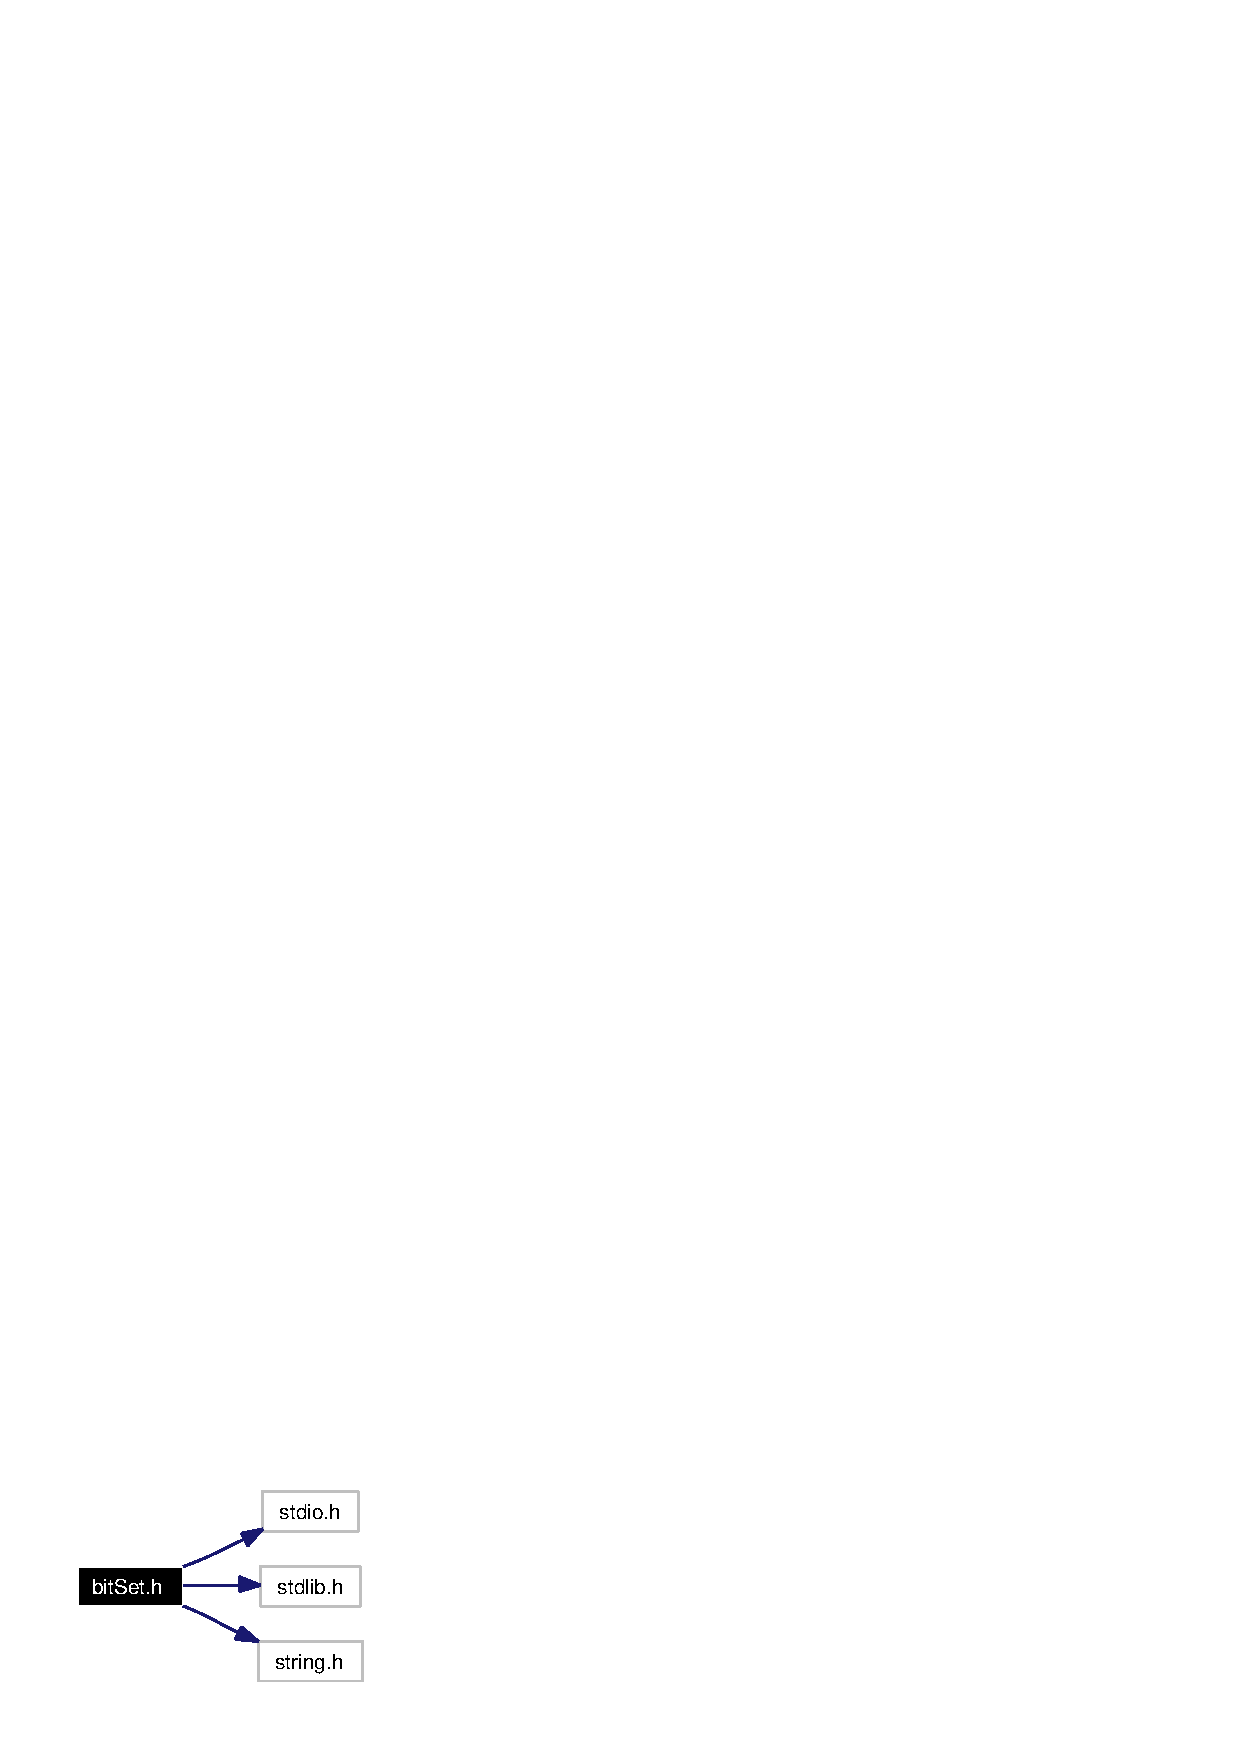
\includegraphics[width=87pt]{bitSet_8h__incl}
\end{center}
\end{figure}


This graph shows which files directly or indirectly include this file:\begin{figure}[H]
\begin{center}
\leavevmode
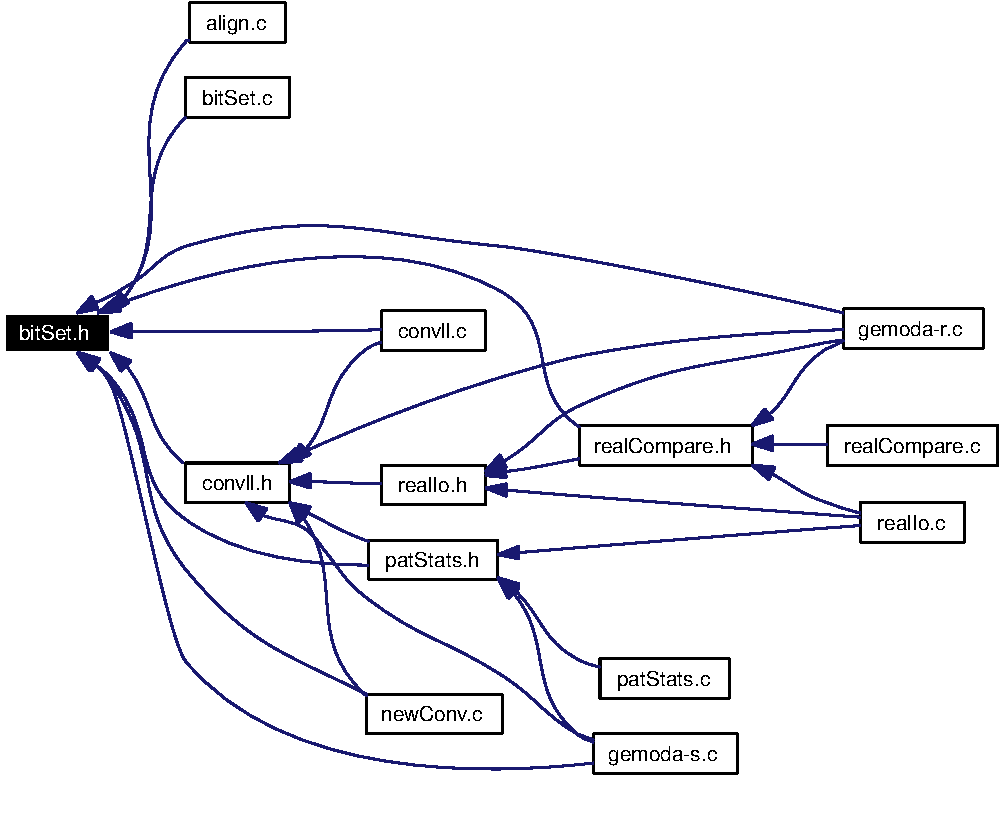
\includegraphics[width=257pt]{bitSet_8h__dep__incl}
\end{center}
\end{figure}
\subsection*{Data Structures}
\begin{CompactItemize}
\item 
struct \hyperlink{structbitSet__t}{bit\-Set\_\-t}
\item 
struct \hyperlink{structbitGraph__t}{bit\-Graph\_\-t}
\end{CompactItemize}
\subsection*{Defines}
\begin{CompactItemize}
\item 
\#define \hyperlink{bitSet_8h_a0}{BSBITSIZE}~(sizeof(\hyperlink{bitSet_8h_a9}{bit\_\-t}) $\ast$ 8)
\begin{CompactList}\small\item\em Get the size of a bit\_\-t, which is an unsigned int. \item\end{CompactList}\item 
\#define \hyperlink{bitSet_8h_a1}{BSMASK}(y)~( ((\hyperlink{bitSet_8h_a9}{bit\_\-t}) 1) $<$$<$ y \% BSBITSIZE )
\item 
\#define \hyperlink{bitSet_8h_a2}{BITSLOT}(y)~( y / BSBITSIZE )
\item 
\#define \hyperlink{bitSet_8h_a3}{BSSET}(x, y)~( x\mbox{[}BITSLOT(y)\mbox{]} $|$= BSMASK(y) )
\begin{CompactList}\small\item\em Sets the y'th bit in x (a bitset\_\-t) to be true using bitwise operators. \item\end{CompactList}\item 
\#define \hyperlink{bitSet_8h_a4}{BSCLEAR}(x, y)~( x\mbox{[}BITSLOT(y)\mbox{]} \&= $\sim$BSMASK(y) )
\begin{CompactList}\small\item\em Sets the y'th bit in x (a bitset\_\-t) to be false using bitwise operators. \item\end{CompactList}\item 
\#define \hyperlink{bitSet_8h_a5}{BSTEST}(x, y)~( x\mbox{[}BITSLOT(y)\mbox{]} \& BSMASK(y) )
\begin{CompactList}\small\item\em Tests whether the y'th bit in x (a bitset\_\-t) is true. \item\end{CompactList}\item 
\#define \hyperlink{bitSet_8h_a6}{BSNUMSLOTS}(n)~((n + BSBITSIZE - 1) / BSBITSIZE)
\item 
\#define \hyperlink{bitSet_8h_a7}{BSUNION}(x, y)~((x)$|$(y))
\begin{CompactList}\small\item\em Performs a union operation on two bit\_\-t's with bitwise operators. \item\end{CompactList}\item 
\#define \hyperlink{bitSet_8h_a8}{BSINTERSECTION}(x, y)~((x)\&(y))
\begin{CompactList}\small\item\em Performs an intersection operation on two bit\_\-t's with bitwise operators. \item\end{CompactList}\end{CompactItemize}
\subsection*{Typedefs}
\begin{CompactItemize}
\item 
typedef unsigned int \hyperlink{bitSet_8h_a9}{bit\_\-t}
\end{CompactItemize}
\subsection*{Functions}
\begin{CompactItemize}
\item 
\hyperlink{bitSet_8h_a9}{bit\_\-t} $\ast$ \hyperlink{bitSet_8h_a10}{new\-Bit\-Array} (int bytes)
\item 
\hyperlink{structbitSet__t}{bit\-Set\_\-t} $\ast$ \hyperlink{bitSet_8h_a11}{new\-Bit\-Set} (int size)
\item 
int \hyperlink{bitSet_8h_a12}{set\-True} (\hyperlink{structbitSet__t}{bit\-Set\_\-t} $\ast$s1, int x)
\item 
int \hyperlink{bitSet_8h_a13}{set\-False} (\hyperlink{structbitSet__t}{bit\-Set\_\-t} $\ast$s1, int x)
\item 
int \hyperlink{bitSet_8h_a14}{bit\-Set\-Difference} (\hyperlink{structbitSet__t}{bit\-Set\_\-t} $\ast$s1, \hyperlink{structbitSet__t}{bit\-Set\_\-t} $\ast$s2, \hyperlink{structbitSet__t}{bit\-Set\_\-t} $\ast$s3)
\item 
int \hyperlink{bitSet_8h_a15}{bit\-Set3Way\-Difference} (\hyperlink{structbitSet__t}{bit\-Set\_\-t} $\ast$s1, \hyperlink{structbitSet__t}{bit\-Set\_\-t} $\ast$s2, \hyperlink{structbitSet__t}{bit\-Set\_\-t} $\ast$s3, \hyperlink{structbitSet__t}{bit\-Set\_\-t} $\ast$s4)
\item 
int \hyperlink{bitSet_8h_a16}{bit\-Set\-Sum} (\hyperlink{structbitSet__t}{bit\-Set\_\-t} $\ast$s1, \hyperlink{structbitSet__t}{bit\-Set\_\-t} $\ast$s2, \hyperlink{structbitSet__t}{bit\-Set\_\-t} $\ast$s3)
\item 
int \hyperlink{bitSet_8h_a17}{flip\-Bits} (\hyperlink{structbitSet__t}{bit\-Set\_\-t} $\ast$s1)
\item 
int \hyperlink{bitSet_8h_a18}{fill\-Set} (\hyperlink{structbitSet__t}{bit\-Set\_\-t} $\ast$s1)
\item 
int \hyperlink{bitSet_8h_a19}{empty\-Set} (\hyperlink{structbitSet__t}{bit\-Set\_\-t} $\ast$s1)
\item 
int \hyperlink{bitSet_8h_a20}{check\-Bit} (\hyperlink{structbitSet__t}{bit\-Set\_\-t} $\ast$s1, int x)
\item 
int \hyperlink{bitSet_8h_a21}{copy\-Bit\-Graph} (\hyperlink{structbitGraph__t}{bit\-Graph\_\-t} $\ast$bg1, \hyperlink{structbitGraph__t}{bit\-Graph\_\-t} $\ast$bg2)
\item 
int \hyperlink{bitSet_8h_a22}{copy\-Set} (\hyperlink{structbitSet__t}{bit\-Set\_\-t} $\ast$s1, \hyperlink{structbitSet__t}{bit\-Set\_\-t} $\ast$s2)
\item 
int \hyperlink{bitSet_8h_a23}{delete\-Bit\-Set} (\hyperlink{structbitSet__t}{bit\-Set\_\-t} $\ast$s1)
\item 
int \hyperlink{bitSet_8h_a24}{bit\-Set\-Union} (\hyperlink{structbitSet__t}{bit\-Set\_\-t} $\ast$s1, \hyperlink{structbitSet__t}{bit\-Set\_\-t} $\ast$s2, \hyperlink{structbitSet__t}{bit\-Set\_\-t} $\ast$s3)
\item 
int \hyperlink{bitSet_8h_a25}{bit\-Set\-Intersection} (\hyperlink{structbitSet__t}{bit\-Set\_\-t} $\ast$s1, \hyperlink{structbitSet__t}{bit\-Set\_\-t} $\ast$s2, \hyperlink{structbitSet__t}{bit\-Set\_\-t} $\ast$s3)
\item 
int \hyperlink{bitSet_8h_a26}{bit\-Set3Way\-Intersection} (\hyperlink{structbitSet__t}{bit\-Set\_\-t} $\ast$s1, \hyperlink{structbitSet__t}{bit\-Set\_\-t} $\ast$s2, \hyperlink{structbitSet__t}{bit\-Set\_\-t} $\ast$s3, \hyperlink{structbitSet__t}{bit\-Set\_\-t} $\ast$s4)
\item 
int \hyperlink{bitSet_8h_a27}{count\-Set} (\hyperlink{structbitSet__t}{bit\-Set\_\-t} $\ast$s1)
\item 
int \hyperlink{bitSet_8h_a28}{fill\-Bit\-Graph} (\hyperlink{structbitGraph__t}{bit\-Graph\_\-t} $\ast$bg1)
\item 
int \hyperlink{bitSet_8h_a29}{empty\-Bit\-Graph} (\hyperlink{structbitGraph__t}{bit\-Graph\_\-t} $\ast$bg1)
\item 
int \hyperlink{bitSet_8h_a30}{print\-Bit\-Set} (\hyperlink{structbitSet__t}{bit\-Set\_\-t} $\ast$s1)
\item 
int \hyperlink{bitSet_8h_a31}{next\-Bit\-Bit\-Set} (\hyperlink{structbitSet__t}{bit\-Set\_\-t} $\ast$s1, int start)
\item 
int \hyperlink{bitSet_8h_a32}{count\-Bit\-Graph\-Non\-Zero} (\hyperlink{structbitGraph__t}{bit\-Graph\_\-t} $\ast$bg)
\item 
int \hyperlink{bitSet_8h_a33}{print\-Binary\-Bit\-Set} (\hyperlink{structbitSet__t}{bit\-Set\_\-t} $\ast$s1)
\item 
int \hyperlink{bitSet_8h_a34}{bit\-Graph\-Set\-True} (\hyperlink{structbitGraph__t}{bit\-Graph\_\-t} $\ast$bg, int x, int y)
\item 
int \hyperlink{bitSet_8h_a35}{bit\-Graph\-Set\-True\-Sym} (\hyperlink{structbitGraph__t}{bit\-Graph\_\-t} $\ast$bg, int x, int y)
\item 
int \hyperlink{bitSet_8h_a36}{bit\-Graph\-Set\-True\-Diagonal} (\hyperlink{structbitGraph__t}{bit\-Graph\_\-t} $\ast$bg)
\item 
int \hyperlink{bitSet_8h_a37}{bit\-Graph\-Set\-False\-Diagonal} (\hyperlink{structbitGraph__t}{bit\-Graph\_\-t} $\ast$bg)
\item 
int \hyperlink{bitSet_8h_a38}{print\-Bit\-Graph} (\hyperlink{structbitGraph__t}{bit\-Graph\_\-t} $\ast$bg)
\item 
\hyperlink{structbitGraph__t}{bit\-Graph\_\-t} $\ast$ \hyperlink{bitSet_8h_a39}{new\-Bit\-Graph} (int size)
\item 
int \hyperlink{bitSet_8h_a40}{delete\-Bit\-Graph} (\hyperlink{structbitGraph__t}{bit\-Graph\_\-t} $\ast$bg)
\item 
int \hyperlink{bitSet_8h_a41}{bit\-Graph\-Row\-Union} (\hyperlink{structbitGraph__t}{bit\-Graph\_\-t} $\ast$bg, int row1, int row2, \hyperlink{structbitSet__t}{bit\-Set\_\-t} $\ast$s1)
\item 
int \hyperlink{bitSet_8h_a42}{bit\-Graph\-Row\-Intersection} (\hyperlink{structbitGraph__t}{bit\-Graph\_\-t} $\ast$bg, int row1, int row2, \hyperlink{structbitSet__t}{bit\-Set\_\-t} $\ast$s1)
\item 
int \hyperlink{bitSet_8h_a43}{bit\-Graph\-Check\-Bit} (\hyperlink{structbitGraph__t}{bit\-Graph\_\-t} $\ast$bg, int x, int y)
\item 
int \hyperlink{bitSet_8h_a44}{bit\-Graph\-Set\-False\-Sym} (\hyperlink{structbitGraph__t}{bit\-Graph\_\-t} $\ast$bg, int x, int y)
\item 
int \hyperlink{bitSet_8h_a45}{bit\-Graph\-Set\-False} (\hyperlink{structbitGraph__t}{bit\-Graph\_\-t} $\ast$bg, int x, int y)
\item 
int \hyperlink{bitSet_8h_a46}{empty\-Bit\-Graph\-Row} (\hyperlink{structbitGraph__t}{bit\-Graph\_\-t} $\ast$bg, int row)
\item 
int \hyperlink{bitSet_8h_a47}{mask\-Bit\-Graph} (\hyperlink{structbitGraph__t}{bit\-Graph\_\-t} $\ast$bg1, \hyperlink{structbitSet__t}{bit\-Set\_\-t} $\ast$bs)
\end{CompactItemize}


\subsection*{Detailed Description}
This file provides declarations and definitions for a bit set object. The functions declared here are defined in \hyperlink{bitSet_8c}{bit\-Set.c}.

Definition in file \hyperlink{bitSet_8h-source}{bit\-Set.h}.

\subsection*{Define Documentation}
\hypertarget{bitSet_8h_a2}{
\index{bitSet.h@{bit\-Set.h}!BITSLOT@{BITSLOT}}
\index{BITSLOT@{BITSLOT}!bitSet.h@{bit\-Set.h}}
\subsubsection[BITSLOT]{\setlength{\rightskip}{0pt plus 5cm}\#define BITSLOT(y)~( y / BSBITSIZE )}}
\label{bitSet_8h_a2}


Finds which bit\_\-t, or \char`\"{}slot\char`\"{}, in a bitset\_\-t the y'th bit belongs to. Also used for testing single bits. 

Definition at line 71 of file bit\-Set.h.

Referenced by next\-Bit\-Bit\-Set().\hypertarget{bitSet_8h_a0}{
\index{bitSet.h@{bit\-Set.h}!BSBITSIZE@{BSBITSIZE}}
\index{BSBITSIZE@{BSBITSIZE}!bitSet.h@{bit\-Set.h}}
\subsubsection[BSBITSIZE]{\setlength{\rightskip}{0pt plus 5cm}\#define BSBITSIZE~(sizeof(\hyperlink{bitSet_8h_a9}{bit\_\-t}) $\ast$ 8)}}
\label{bitSet_8h_a0}




Definition at line 63 of file bit\-Set.h.

Referenced by next\-Bit\-Bit\-Set().\hypertarget{bitSet_8h_a4}{
\index{bitSet.h@{bit\-Set.h}!BSCLEAR@{BSCLEAR}}
\index{BSCLEAR@{BSCLEAR}!bitSet.h@{bit\-Set.h}}
\subsubsection[BSCLEAR]{\setlength{\rightskip}{0pt plus 5cm}\#define BSCLEAR(x, y)~( x\mbox{[}BITSLOT(y)\mbox{]} \&= $\sim$BSMASK(y) )}}
\label{bitSet_8h_a4}




Definition at line 77 of file bit\-Set.h.

Referenced by set\-False().\hypertarget{bitSet_8h_a8}{
\index{bitSet.h@{bit\-Set.h}!BSINTERSECTION@{BSINTERSECTION}}
\index{BSINTERSECTION@{BSINTERSECTION}!bitSet.h@{bit\-Set.h}}
\subsubsection[BSINTERSECTION]{\setlength{\rightskip}{0pt plus 5cm}\#define BSINTERSECTION(x, y)~((x)\&(y))}}
\label{bitSet_8h_a8}




Definition at line 93 of file bit\-Set.h.

Referenced by bit\-Set3Way\-Intersection(), and bit\-Set\-Intersection().\hypertarget{bitSet_8h_a1}{
\index{bitSet.h@{bit\-Set.h}!BSMASK@{BSMASK}}
\index{BSMASK@{BSMASK}!bitSet.h@{bit\-Set.h}}
\subsubsection[BSMASK]{\setlength{\rightskip}{0pt plus 5cm}\#define BSMASK(y)~( ((\hyperlink{bitSet_8h_a9}{bit\_\-t}) 1) $<$$<$ y \% BSBITSIZE )}}
\label{bitSet_8h_a1}


Uses bit operations to make a mask the size of a bit\_\-t with the y'th bit true and all other bits false. Used for testing a single bit. 

Definition at line 67 of file bit\-Set.h.\hypertarget{bitSet_8h_a6}{
\index{bitSet.h@{bit\-Set.h}!BSNUMSLOTS@{BSNUMSLOTS}}
\index{BSNUMSLOTS@{BSNUMSLOTS}!bitSet.h@{bit\-Set.h}}
\subsubsection[BSNUMSLOTS]{\setlength{\rightskip}{0pt plus 5cm}\#define BSNUMSLOTS(n)~((n + BSBITSIZE - 1) / BSBITSIZE)}}
\label{bitSet_8h_a6}


Finds the total number of bit\_\-t's (\char`\"{}slot\char`\"{}s) that are necessary for a bitset of length n. Uses integer division and supplements by BSBITSIZE - 1 to make sure that for slots that are less than full, a slot is still allocated, and for slots that are full, no extra slot is allocated. 

Definition at line 87 of file bit\-Set.h.

Referenced by new\-Bit\-Set().\hypertarget{bitSet_8h_a3}{
\index{bitSet.h@{bit\-Set.h}!BSSET@{BSSET}}
\index{BSSET@{BSSET}!bitSet.h@{bit\-Set.h}}
%\subsubsection[BSSET]{\setlength{\rightskip}{0pt plus 5cm}\#define BSSET(x, y)~( x\mbox{[}BITSLOT(y)\mbox{]} $|$= BSMASK(y) )}}
\label{bitSet_8h_a3}




Definition at line 74 of file bit\-Set.h.

Referenced by set\-True().\hypertarget{bitSet_8h_a5}{
\index{bitSet.h@{bit\-Set.h}!BSTEST@{BSTEST}}
\index{BSTEST@{BSTEST}!bitSet.h@{bit\-Set.h}}
\subsubsection[BSTEST]{\setlength{\rightskip}{0pt plus 5cm}\#define BSTEST(x, y)~( x\mbox{[}BITSLOT(y)\mbox{]} \& BSMASK(y) )}}
\label{bitSet_8h_a5}




Definition at line 80 of file bit\-Set.h.

Referenced by check\-Bit(), print\-Binary\-Bit\-Set(), and print\-Bit\-Set().\hypertarget{bitSet_8h_a7}{
\index{bitSet.h@{bit\-Set.h}!BSUNION@{BSUNION}}
\index{BSUNION@{BSUNION}!bitSet.h@{bit\-Set.h}}
\subsubsection[BSUNION]{\setlength{\rightskip}{0pt plus 5cm}\#define BSUNION(x, y)~((x)$|$(y))}}
\label{bitSet_8h_a7}




Definition at line 90 of file bit\-Set.h.

Referenced by bit\-Set\-Union().

\subsection*{Typedef Documentation}
\hypertarget{bitSet_8h_a9}{
\index{bitSet.h@{bit\-Set.h}!bit_t@{bit\_\-t}}
\index{bit_t@{bit\_\-t}!bitSet.h@{bit\-Set.h}}
\subsubsection[bit\_\-t]{\setlength{\rightskip}{0pt plus 5cm}typedef unsigned int \hyperlink{bitSet_8h_a9}{bit\_\-t}}}
\label{bitSet_8h_a9}


a bit\_\-t is the size of an unsigned integer on the current architecture.

Definition at line 15 of file bit\-Set.h.

\subsection*{Function Documentation}
\hypertarget{bitSet_8h_a43}{
\index{bitSet.h@{bit\-Set.h}!bitGraphCheckBit@{bitGraphCheckBit}}
\index{bitGraphCheckBit@{bitGraphCheckBit}!bitSet.h@{bit\-Set.h}}
\subsubsection[bitGraphCheckBit]{\setlength{\rightskip}{0pt plus 5cm}int bit\-Graph\-Check\-Bit (\hyperlink{structbitGraph__t}{bit\-Graph\_\-t} $\ast$ {\em bg}, int {\em x}, int {\em y})}}
\label{bitSet_8h_a43}


Checks the value of a bit in a \hyperlink{structbitGraph__t}{bit\-Graph\_\-t} object. Input: a \hyperlink{structbitGraph__t}{bit\-Graph\_\-t} object, the index of the row of the \hyperlink{structbitGraph__t}{bit\-Graph\_\-t} with the bit to be checked, the index of the bit in that row that is to be checked. Output: the value of the bit in the bit\-Graph being checked.

Definition at line 599 of file bit\-Set.c.

References check\-Bit(), and bit\-Graph\_\-t::graph.

Referenced by main(), and measure\-Diagonal().



\hypertarget{bitSet_8h_a42}{
\index{bitSet.h@{bit\-Set.h}!bitGraphRowIntersection@{bitGraphRowIntersection}}
\index{bitGraphRowIntersection@{bitGraphRowIntersection}!bitSet.h@{bit\-Set.h}}
\subsubsection[bitGraphRowIntersection]{\setlength{\rightskip}{0pt plus 5cm}int bit\-Graph\-Row\-Intersection (\hyperlink{structbitGraph__t}{bit\-Graph\_\-t} $\ast$ {\em bg}, int {\em row1}, int {\em row2}, \hyperlink{structbitSet__t}{bit\-Set\_\-t} $\ast$ {\em s1})}}
\label{bitSet_8h_a42}


Finds the intersection of two rows (bit\-Sets) within a \hyperlink{structbitGraph__t}{bit\-Graph\_\-t} object. Input: a \hyperlink{structbitGraph__t}{bit\-Graph\_\-t} object, first row to be compared, second row to be compared, and a \hyperlink{structbitSet__t}{bit\-Set\_\-t} to store the intersection results. Output: integer success value of 0 (and an altered destination \hyperlink{structbitSet__t}{bit\-Set\_\-t} object with a true value wherever both source bit\-Sets had a true value).

Definition at line 572 of file bit\-Set.c.

References bit\-Set\-Intersection(), and bit\-Graph\_\-t::graph.

Referenced by get\-Stat\-Mat(), and old\-Get\-Stat\-Mat().



\hypertarget{bitSet_8h_a41}{
\index{bitSet.h@{bit\-Set.h}!bitGraphRowUnion@{bitGraphRowUnion}}
\index{bitGraphRowUnion@{bitGraphRowUnion}!bitSet.h@{bit\-Set.h}}
\subsubsection[bitGraphRowUnion]{\setlength{\rightskip}{0pt plus 5cm}int bit\-Graph\-Row\-Union (\hyperlink{structbitGraph__t}{bit\-Graph\_\-t} $\ast$ {\em bg}, int {\em row1}, int {\em row2}, \hyperlink{structbitSet__t}{bit\-Set\_\-t} $\ast$ {\em s1})}}
\label{bitSet_8h_a41}


Finds the union of two rows (bit\-Sets) within a bit\-Graph Input: a \hyperlink{structbitGraph__t}{bit\-Graph\_\-t} object, first row to be compared, second row to be compared, and a \hyperlink{structbitSet__t}{bit\-Set\_\-t} to store the union results. Output: integer success value of 0 (and an altered destination \hyperlink{structbitSet__t}{bit\-Set\_\-t} object with a true value wherever one or both source bit\-Sets had a true value).

Definition at line 560 of file bit\-Set.c.

References bit\-Set\-Union(), and bit\-Graph\_\-t::graph.



\hypertarget{bitSet_8h_a45}{
\index{bitSet.h@{bit\-Set.h}!bitGraphSetFalse@{bitGraphSetFalse}}
\index{bitGraphSetFalse@{bitGraphSetFalse}!bitSet.h@{bit\-Set.h}}
\subsubsection[bitGraphSetFalse]{\setlength{\rightskip}{0pt plus 5cm}int bit\-Graph\-Set\-False (\hyperlink{structbitGraph__t}{bit\-Graph\_\-t} $\ast$ {\em bg}, int {\em x}, int {\em y})}}
\label{bitSet_8h_a45}


Sets a specific bit in a bit\-Graph false. Input: a \hyperlink{structbitGraph__t}{bit\-Graph\_\-t} object, the index of the row of the \hyperlink{structbitGraph__t}{bit\-Graph\_\-t} with the bit be set, the index of the bit in that row that is to be set. Output: integer success value of 0 (and an altered \hyperlink{structbitGraph__t}{bit\-Graph\_\-t} object).

Definition at line 623 of file bit\-Set.c.

References bit\-Graph\_\-t::graph, and set\-False().



\hypertarget{bitSet_8h_a37}{
\index{bitSet.h@{bit\-Set.h}!bitGraphSetFalseDiagonal@{bitGraphSetFalseDiagonal}}
\index{bitGraphSetFalseDiagonal@{bitGraphSetFalseDiagonal}!bitSet.h@{bit\-Set.h}}
\subsubsection[bitGraphSetFalseDiagonal]{\setlength{\rightskip}{0pt plus 5cm}int bit\-Graph\-Set\-False\-Diagonal (\hyperlink{structbitGraph__t}{bit\-Graph\_\-t} $\ast$ {\em bg})}}
\label{bitSet_8h_a37}


Sets the main diagonal of a bit\-Graph false. Input: a \hyperlink{structbitGraph__t}{bit\-Graph\_\-t} object. Output: integer success value of 0 (and an altered \hyperlink{structbitGraph__t}{bit\-Graph\_\-t} object).

Definition at line 678 of file bit\-Set.c.

References bit\-Graph\_\-t::graph, and set\-False().

Referenced by convolve().



\hypertarget{bitSet_8h_a44}{
\index{bitSet.h@{bit\-Set.h}!bitGraphSetFalseSym@{bitGraphSetFalseSym}}
\index{bitGraphSetFalseSym@{bitGraphSetFalseSym}!bitSet.h@{bit\-Set.h}}
\subsubsection[bitGraphSetFalseSym]{\setlength{\rightskip}{0pt plus 5cm}int bit\-Graph\-Set\-False\-Sym (\hyperlink{structbitGraph__t}{bit\-Graph\_\-t} $\ast$ {\em bg}, int {\em x}, int {\em y})}}
\label{bitSet_8h_a44}


Sets a specific bit and its symmetric opposite in a bit\-Graph false. For instance, given that we wanted to set the 3rd bit in the 5th row false, this would also set the 5th bit in the 3rd row. Input: a \hyperlink{structbitGraph__t}{bit\-Graph\_\-t} object, the index of the row of the bit\-Graph with the bit be set, the index of the bit in that row that is to be set. Output: integer success value of 0 (and an altered \hyperlink{structbitGraph__t}{bit\-Graph\_\-t} object).

Definition at line 637 of file bit\-Set.c.

References bit\-Graph\_\-t::graph, and set\-False().



\hypertarget{bitSet_8h_a34}{
\index{bitSet.h@{bit\-Set.h}!bitGraphSetTrue@{bitGraphSetTrue}}
\index{bitGraphSetTrue@{bitGraphSetTrue}!bitSet.h@{bit\-Set.h}}
\subsubsection[bitGraphSetTrue]{\setlength{\rightskip}{0pt plus 5cm}int bit\-Graph\-Set\-True (\hyperlink{structbitGraph__t}{bit\-Graph\_\-t} $\ast$ {\em bg}, int {\em x}, int {\em y})}}
\label{bitSet_8h_a34}


Sets a specific bit in a bit\-Graph true. Input: a \hyperlink{structbitGraph__t}{bit\-Graph\_\-t} object, the index of the row of the \hyperlink{structbitGraph__t}{bit\-Graph\_\-t} with the bit be set, the index of the bit in that row that is to be set. Output: integer success value of 0 (and an altered \hyperlink{structbitGraph__t}{bit\-Graph\_\-t} object).

Definition at line 611 of file bit\-Set.c.

References bit\-Graph\_\-t::graph, and set\-True().



\hypertarget{bitSet_8h_a36}{
\index{bitSet.h@{bit\-Set.h}!bitGraphSetTrueDiagonal@{bitGraphSetTrueDiagonal}}
\index{bitGraphSetTrueDiagonal@{bitGraphSetTrueDiagonal}!bitSet.h@{bit\-Set.h}}
\subsubsection[bitGraphSetTrueDiagonal]{\setlength{\rightskip}{0pt plus 5cm}int bit\-Graph\-Set\-True\-Diagonal (\hyperlink{structbitGraph__t}{bit\-Graph\_\-t} $\ast$ {\em bg})}}
\label{bitSet_8h_a36}


Sets the main diagonal of a bit\-Graph true. Input: a \hyperlink{structbitGraph__t}{bit\-Graph\_\-t} object. Output: integer success value of 0 (and an altered \hyperlink{structbitGraph__t}{bit\-Graph\_\-t} object).

Definition at line 664 of file bit\-Set.c.

References bit\-Graph\_\-t::graph, and set\-True().



\hypertarget{bitSet_8h_a35}{
\index{bitSet.h@{bit\-Set.h}!bitGraphSetTrueSym@{bitGraphSetTrueSym}}
\index{bitGraphSetTrueSym@{bitGraphSetTrueSym}!bitSet.h@{bit\-Set.h}}
\subsubsection[bitGraphSetTrueSym]{\setlength{\rightskip}{0pt plus 5cm}int bit\-Graph\-Set\-True\-Sym (\hyperlink{structbitGraph__t}{bit\-Graph\_\-t} $\ast$ {\em bg}, int {\em x}, int {\em y})}}
\label{bitSet_8h_a35}


Sets a specific bit and its symmetric opposite in a bit\-Graph true. For instance, given that we wanted to set the 3rd bit in the 5th row true, this would also set the 5th bit in the 3rd row. Input: a bit\-Graph, the index of the row of the bit\-Graph with the bit be set, the index of the bit in that row that is to be set. Output: integer success value of 0 (and an altered \hyperlink{structbitGraph__t}{bit\-Graph\_\-t} object).

Definition at line 652 of file bit\-Set.c.

References bit\-Graph\_\-t::graph, and set\-True().

Referenced by align\-Words\-Mat\_\-bit(), main(), and real\-Comparison().



\hypertarget{bitSet_8h_a15}{
\index{bitSet.h@{bit\-Set.h}!bitSet3WayDifference@{bitSet3WayDifference}}
\index{bitSet3WayDifference@{bitSet3WayDifference}!bitSet.h@{bit\-Set.h}}
\subsubsection[bitSet3WayDifference]{\setlength{\rightskip}{0pt plus 5cm}int bit\-Set3Way\-Difference (\hyperlink{structbitSet__t}{bit\-Set\_\-t} $\ast$ {\em s1}, \hyperlink{structbitSet__t}{bit\-Set\_\-t} $\ast$ {\em s2}, \hyperlink{structbitSet__t}{bit\-Set\_\-t} $\ast$ {\em s3}, \hyperlink{structbitSet__t}{bit\-Set\_\-t} $\ast$ {\em s4})}}
\label{bitSet_8h_a15}


\hypertarget{bitSet_8h_a26}{
\index{bitSet.h@{bit\-Set.h}!bitSet3WayIntersection@{bitSet3WayIntersection}}
\index{bitSet3WayIntersection@{bitSet3WayIntersection}!bitSet.h@{bit\-Set.h}}
\subsubsection[bitSet3WayIntersection]{\setlength{\rightskip}{0pt plus 5cm}int bit\-Set3Way\-Intersection (\hyperlink{structbitSet__t}{bit\-Set\_\-t} $\ast$ {\em s1}, \hyperlink{structbitSet__t}{bit\-Set\_\-t} $\ast$ {\em s2}, \hyperlink{structbitSet__t}{bit\-Set\_\-t} $\ast$ {\em s3}, \hyperlink{structbitSet__t}{bit\-Set\_\-t} $\ast$ {\em s4})}}
\label{bitSet_8h_a26}


Finds the intersection of 3 bit\-Sets. Input: First bit\-Set to be intersected, second bitset to be intersected. third bit\-Set to be intersected, a bit\-Set to store the result of the intersection. Output: Integer success value of 0 (and an altered destination \hyperlink{structbitSet__t}{bit\-Set\_\-t} object with a true where all three source bit\-Sets had a true.)

Definition at line 304 of file bit\-Set.c.

References BSINTERSECTION, bit\-Set\_\-t::slots, and bit\-Set\_\-t::tf.



\hypertarget{bitSet_8h_a14}{
\index{bitSet.h@{bit\-Set.h}!bitSetDifference@{bitSetDifference}}
\index{bitSetDifference@{bitSetDifference}!bitSet.h@{bit\-Set.h}}
\subsubsection[bitSetDifference]{\setlength{\rightskip}{0pt plus 5cm}int bit\-Set\-Difference (\hyperlink{structbitSet__t}{bit\-Set\_\-t} $\ast$ {\em s1}, \hyperlink{structbitSet__t}{bit\-Set\_\-t} $\ast$ {\em s2}, \hyperlink{structbitSet__t}{bit\-Set\_\-t} $\ast$ {\em s3})}}
\label{bitSet_8h_a14}


Locates all differences between two bit\-Sets. The result bit\-Set contains a true at a given bit if the two source bit\-Sets differ at that bit. Input: first bit set to be compared, second bit set to be compared. third bit set to store the results Output: integer success value of 0 (and an altered destination \hyperlink{structbitSet__t}{bit\-Set\_\-t} object with a true where the two source bit sets differed).

Definition at line 237 of file bit\-Set.c.

References bit\-Set\_\-t::slots, and bit\-Set\_\-t::tf.



\hypertarget{bitSet_8h_a25}{
\index{bitSet.h@{bit\-Set.h}!bitSetIntersection@{bitSetIntersection}}
\index{bitSetIntersection@{bitSetIntersection}!bitSet.h@{bit\-Set.h}}
\subsubsection[bitSetIntersection]{\setlength{\rightskip}{0pt plus 5cm}int bit\-Set\-Intersection (\hyperlink{structbitSet__t}{bit\-Set\_\-t} $\ast$ {\em s1}, \hyperlink{structbitSet__t}{bit\-Set\_\-t} $\ast$ {\em s2}, \hyperlink{structbitSet__t}{bit\-Set\_\-t} $\ast$ {\em s3})}}
\label{bitSet_8h_a25}


Finds the intersection of two bitsets. Input: First bit\-Set to be intersected, second bit\-Set to be intersected. a bit\-Set to store the result of the intersection. Output: Integer success value of 0 (and an altered destination \hyperlink{structbitSet__t}{bit\-Set\_\-t} object. with a true where both source bit\-Sets had a true).

Definition at line 278 of file bit\-Set.c.

References BSINTERSECTION, bit\-Set\_\-t::slots, and bit\-Set\_\-t::tf.

Referenced by bit\-Graph\-Row\-Intersection(), find\-Cliques(), and mask\-Bit\-Graph().



\hypertarget{bitSet_8h_a16}{
\index{bitSet.h@{bit\-Set.h}!bitSetSum@{bitSetSum}}
\index{bitSetSum@{bitSetSum}!bitSet.h@{bit\-Set.h}}
\subsubsection[bitSetSum]{\setlength{\rightskip}{0pt plus 5cm}int bit\-Set\-Sum (\hyperlink{structbitSet__t}{bit\-Set\_\-t} $\ast$ {\em s1}, \hyperlink{structbitSet__t}{bit\-Set\_\-t} $\ast$ {\em s2}, \hyperlink{structbitSet__t}{bit\-Set\_\-t} $\ast$ {\em s3})}}
\label{bitSet_8h_a16}


Adds two \hyperlink{structbitSet__t}{bit\-Set\_\-t} objects together. Currently unknown functionality, not used in existing code.

Definition at line 256 of file bit\-Set.c.

References bit\-Set\_\-t::slots, and bit\-Set\_\-t::tf.



\hypertarget{bitSet_8h_a24}{
\index{bitSet.h@{bit\-Set.h}!bitSetUnion@{bitSetUnion}}
\index{bitSetUnion@{bitSetUnion}!bitSet.h@{bit\-Set.h}}
\subsubsection[bitSetUnion]{\setlength{\rightskip}{0pt plus 5cm}int bit\-Set\-Union (\hyperlink{structbitSet__t}{bit\-Set\_\-t} $\ast$ {\em s1}, \hyperlink{structbitSet__t}{bit\-Set\_\-t} $\ast$ {\em s2}, \hyperlink{structbitSet__t}{bit\-Set\_\-t} $\ast$ {\em s3})}}
\label{bitSet_8h_a24}


Finds the union of two bit\-Sets Input: first bit set for the union, second bit set for the union. a bit set in which to store the results Output: an integer success value of 0 (and an altered third \hyperlink{structbitSet__t}{bit\-Set\_\-t} with the results of the union.

Definition at line 175 of file bit\-Set.c.

References BSUNION, bit\-Set\_\-t::slots, and bit\-Set\_\-t::tf.

Referenced by bit\-Graph\-Row\-Union(), and single\-Linkage().



\hypertarget{bitSet_8h_a20}{
\index{bitSet.h@{bit\-Set.h}!checkBit@{checkBit}}
\index{checkBit@{checkBit}!bitSet.h@{bit\-Set.h}}
\subsubsection[checkBit]{\setlength{\rightskip}{0pt plus 5cm}int check\-Bit (\hyperlink{structbitSet__t}{bit\-Set\_\-t} $\ast$ {\em s1}, int {\em x})}}
\label{bitSet_8h_a20}


Finds the value of a specific bit in a bit\-Set. Input: a bit\-Set, the number of the bit being queried. Output: the value of the bit being queried (1 or 0).

Definition at line 143 of file bit\-Set.c.

References BSTEST, and bit\-Set\_\-t::tf.

Referenced by bit\-Graph\-Check\-Bit(), find\-Cliques(), get\-Stat\-Mat(), mask\-Bit\-Graph(), next\-Bit\-Bit\-Set(), single\-Linkage(), and whole\-Round\-Conv().



\hypertarget{bitSet_8h_a21}{
\index{bitSet.h@{bit\-Set.h}!copyBitGraph@{copyBitGraph}}
\index{copyBitGraph@{copyBitGraph}!bitSet.h@{bit\-Set.h}}
\subsubsection[copyBitGraph]{\setlength{\rightskip}{0pt plus 5cm}int copy\-Bit\-Graph (\hyperlink{structbitGraph__t}{bit\-Graph\_\-t} $\ast$ {\em bg1}, \hyperlink{structbitGraph__t}{bit\-Graph\_\-t} $\ast$ {\em bg2})}}
\label{bitSet_8h_a21}


Copies the true/false contents of one bit graph into an existing bit graph. Both bit graphs must be the same size, and each corresponding bit set between the two bit graphs must be the same size. Input: source bit graph, destination \hyperlink{structbitGraph__t}{bit\-Graph\_\-t} object. Output: integer success value of 0 (and an altered destination bit graph).

Definition at line 215 of file bit\-Set.c.

References copy\-Set(), bit\-Graph\_\-t::graph, and bit\-Graph\_\-t::size.



\hypertarget{bitSet_8h_a22}{
\index{bitSet.h@{bit\-Set.h}!copySet@{copySet}}
\index{copySet@{copySet}!bitSet.h@{bit\-Set.h}}
\subsubsection[copySet]{\setlength{\rightskip}{0pt plus 5cm}int copy\-Set (\hyperlink{structbitSet__t}{bit\-Set\_\-t} $\ast$ {\em s1}, \hyperlink{structbitSet__t}{bit\-Set\_\-t} $\ast$ {\em s2})}}
\label{bitSet_8h_a22}


Copies the true/false contents of one bit set into an existing bit set. Both bit sets must be the same size. Input: source bit set, destination \hyperlink{structbitSet__t}{bit\-Set\_\-t} object. Output: integer success value of 0 (and an altered destination bitset.

Definition at line 195 of file bit\-Set.c.

References bit\-Set\_\-t::slots, and bit\-Set\_\-t::tf.

Referenced by copy\-Bit\-Graph(), filter\-Graph(), and single\-Linkage().



\hypertarget{bitSet_8h_a32}{
\index{bitSet.h@{bit\-Set.h}!countBitGraphNonZero@{countBitGraphNonZero}}
\index{countBitGraphNonZero@{countBitGraphNonZero}!bitSet.h@{bit\-Set.h}}
\subsubsection[countBitGraphNonZero]{\setlength{\rightskip}{0pt plus 5cm}int count\-Bit\-Graph\-Non\-Zero (\hyperlink{structbitGraph__t}{bit\-Graph\_\-t} $\ast$ {\em bg})}}
\label{bitSet_8h_a32}


Counts the number of true (non-zero) values in a \hyperlink{structbitGraph__t}{bit\-Graph\_\-t} object. Input: a \hyperlink{structbitGraph__t}{bit\-Graph\_\-t} object. Output: the integer number of true (non-zero) values in the \hyperlink{structbitGraph__t}{bit\-Graph\_\-t} object.

Definition at line 511 of file bit\-Set.c.

References count\-Set(), and bit\-Graph\_\-t::graph.



\hypertarget{bitSet_8h_a27}{
\index{bitSet.h@{bit\-Set.h}!countSet@{countSet}}
\index{countSet@{countSet}!bitSet.h@{bit\-Set.h}}
\subsubsection[countSet]{\setlength{\rightskip}{0pt plus 5cm}int count\-Set (\hyperlink{structbitSet__t}{bit\-Set\_\-t} $\ast$ {\em s1})}}
\label{bitSet_8h_a27}


Counts the number of true values in a bit\-Set. Input: a \hyperlink{structbitSet__t}{bit\-Set\_\-t} object. Output: number of true values in that \hyperlink{structbitSet__t}{bit\-Set\_\-t} object.

Definition at line 413 of file bit\-Set.c.

References bitcount32\_\-precomp(), and bit\-Set\_\-t::tf.

Referenced by bit\-Set\-To\-CSet(), count\-Bit\-Graph\-Non\-Zero(), filter\-Graph(), filter\-Iter(), find\-Cliques(), get\-Stat\-Mat(), old\-Get\-Stat\-Mat(), print\-Bit\-Set(), single\-Linkage(), and whole\-Clique\-Conv().



\hypertarget{bitSet_8h_a40}{
\index{bitSet.h@{bit\-Set.h}!deleteBitGraph@{deleteBitGraph}}
\index{deleteBitGraph@{deleteBitGraph}!bitSet.h@{bit\-Set.h}}
\subsubsection[deleteBitGraph]{\setlength{\rightskip}{0pt plus 5cm}int delete\-Bit\-Graph (\hyperlink{structbitGraph__t}{bit\-Graph\_\-t} $\ast$ {\em bg})}}
\label{bitSet_8h_a40}


Deletes a \hyperlink{structbitGraph__t}{bit\-Graph\_\-t} object from memory. Input: a \hyperlink{structbitGraph__t}{bit\-Graph\_\-t} object to be deleted. Output: integer success value from 0 (and deletion of a \hyperlink{structbitGraph__t}{bit\-Graph\_\-t} object).

Definition at line 799 of file bit\-Set.c.

References delete\-Bit\-Set(), and bit\-Graph\_\-t::graph.

Referenced by main().



\hypertarget{bitSet_8h_a23}{
\index{bitSet.h@{bit\-Set.h}!deleteBitSet@{deleteBitSet}}
\index{deleteBitSet@{deleteBitSet}!bitSet.h@{bit\-Set.h}}
\subsubsection[deleteBitSet]{\setlength{\rightskip}{0pt plus 5cm}int delete\-Bit\-Set (\hyperlink{structbitSet__t}{bit\-Set\_\-t} $\ast$ {\em s1})}}
\label{bitSet_8h_a23}


Performs memory management for the deletion of a \hyperlink{structbitSet__t}{bit\-Set\_\-t} structure. Input: a \hyperlink{structbitSet__t}{bit\-Set\_\-t} object. Output: integer success value of 1.

Definition at line 154 of file bit\-Set.c.

References bit\-Set\_\-t::tf.

Referenced by convolve(), delete\-Bit\-Graph(), filter\-Graph(), find\-Cliques(), get\-Stat\-Mat(), old\-Get\-Stat\-Mat(), whole\-Clique\-Conv(), and whole\-Round\-Conv().



\hypertarget{bitSet_8h_a29}{
\index{bitSet.h@{bit\-Set.h}!emptyBitGraph@{emptyBitGraph}}
\index{emptyBitGraph@{emptyBitGraph}!bitSet.h@{bit\-Set.h}}
\subsubsection[emptyBitGraph]{\setlength{\rightskip}{0pt plus 5cm}int empty\-Bit\-Graph (\hyperlink{structbitGraph__t}{bit\-Graph\_\-t} $\ast$ {\em bg1})}}
\label{bitSet_8h_a29}


Sets all bits in the \hyperlink{structbitGraph__t}{bit\-Graph\_\-t} object to false. Input: a \hyperlink{structbitGraph__t}{bit\-Graph\_\-t} object. Output: integer success value of 0 (and a \hyperlink{structbitGraph__t}{bit\-Graph\_\-t} with all false bits).

Definition at line 744 of file bit\-Set.c.

References empty\-Set(), and bit\-Graph\_\-t::graph.



\hypertarget{bitSet_8h_a46}{
\index{bitSet.h@{bit\-Set.h}!emptyBitGraphRow@{emptyBitGraphRow}}
\index{emptyBitGraphRow@{emptyBitGraphRow}!bitSet.h@{bit\-Set.h}}
\subsubsection[emptyBitGraphRow]{\setlength{\rightskip}{0pt plus 5cm}int empty\-Bit\-Graph\-Row (\hyperlink{structbitGraph__t}{bit\-Graph\_\-t} $\ast$ {\em bg}, int {\em row})}}
\label{bitSet_8h_a46}


Sets all bits in a \hyperlink{structbitGraph__t}{bit\-Graph\_\-t} row (a \hyperlink{structbitSet__t}{bit\-Set\_\-t} object) false. Input: a bit\-Graph, a row in the \hyperlink{structbitGraph__t}{bit\-Graph\_\-t} object to be emptied. Output: integer success value of 0 (and an altered \hyperlink{structbitGraph__t}{bit\-Graph\_\-t} object).

Definition at line 788 of file bit\-Set.c.

References empty\-Set(), and bit\-Graph\_\-t::graph.



\hypertarget{bitSet_8h_a19}{
\index{bitSet.h@{bit\-Set.h}!emptySet@{emptySet}}
\index{emptySet@{emptySet}!bitSet.h@{bit\-Set.h}}
\subsubsection[emptySet]{\setlength{\rightskip}{0pt plus 5cm}int empty\-Set (\hyperlink{structbitSet__t}{bit\-Set\_\-t} $\ast$ {\em s1})}}
\label{bitSet_8h_a19}


Sets all values in a bit\-Set to false. Input: a \hyperlink{structbitSet__t}{bit\-Set\_\-t} object. Output: integer success value of 1.

Definition at line 131 of file bit\-Set.c.

References bit\-Set\_\-t::bytes, and bit\-Set\_\-t::tf.

Referenced by empty\-Bit\-Graph(), empty\-Bit\-Graph\-Row(), filter\-Graph(), filter\-Iter(), mask\-Bit\-Graph(), prune\-Bit\-Graph(), and search\-Mems\-With\-List().



\hypertarget{bitSet_8h_a28}{
\index{bitSet.h@{bit\-Set.h}!fillBitGraph@{fillBitGraph}}
\index{fillBitGraph@{fillBitGraph}!bitSet.h@{bit\-Set.h}}
\subsubsection[fillBitGraph]{\setlength{\rightskip}{0pt plus 5cm}int fill\-Bit\-Graph (\hyperlink{structbitGraph__t}{bit\-Graph\_\-t} $\ast$ {\em bg1})}}
\label{bitSet_8h_a28}


Sets all bits in the \hyperlink{structbitGraph__t}{bit\-Graph\_\-t} object to true. Input: a \hyperlink{structbitGraph__t}{bit\-Graph\_\-t} object. Output: integer success value of 0 (and a \hyperlink{structbitGraph__t}{bit\-Graph\_\-t} object with all true bits).

Definition at line 730 of file bit\-Set.c.

References fill\-Set(), and bit\-Graph\_\-t::graph.



\hypertarget{bitSet_8h_a18}{
\index{bitSet.h@{bit\-Set.h}!fillSet@{fillSet}}
\index{fillSet@{fillSet}!bitSet.h@{bit\-Set.h}}
\subsubsection[fillSet]{\setlength{\rightskip}{0pt plus 5cm}int fill\-Set (\hyperlink{structbitSet__t}{bit\-Set\_\-t} $\ast$ {\em s1})}}
\label{bitSet_8h_a18}


Sets all values in a bit\-Set to true. Input: a bit\-Set. Output: integer success value of 1.

Definition at line 119 of file bit\-Set.c.

References bit\-Set\_\-t::bytes, and bit\-Set\_\-t::tf.

Referenced by convolve(), fill\-Bit\-Graph(), and whole\-Round\-Conv().



\hypertarget{bitSet_8h_a17}{
\index{bitSet.h@{bit\-Set.h}!flipBits@{flipBits}}
\index{flipBits@{flipBits}!bitSet.h@{bit\-Set.h}}
\subsubsection[flipBits]{\setlength{\rightskip}{0pt plus 5cm}int flip\-Bits (\hyperlink{structbitSet__t}{bit\-Set\_\-t} $\ast$ {\em s1})}}
\label{bitSet_8h_a17}


Inverts all values in a bit\-Set, making all trues false and all falses true. Input: a bit\-Set. Output: integer success value of 1.

Definition at line 105 of file bit\-Set.c.

References bit\-Set\_\-t::tf.



\hypertarget{bitSet_8h_a47}{
\index{bitSet.h@{bit\-Set.h}!maskBitGraph@{maskBitGraph}}
\index{maskBitGraph@{maskBitGraph}!bitSet.h@{bit\-Set.h}}
\subsubsection[maskBitGraph]{\setlength{\rightskip}{0pt plus 5cm}int mask\-Bit\-Graph (\hyperlink{structbitGraph__t}{bit\-Graph\_\-t} $\ast$ {\em bg1}, \hyperlink{structbitSet__t}{bit\-Set\_\-t} $\ast$ {\em bs})}}
\label{bitSet_8h_a47}


Makes a bit\-Graph contain only true bits according to the bitmask given. Only locations with the row and column both true in the bitmask can be true if they were initially true. If they were false, they remain false. If the location does not have both the row and the column in the bitmask, it is made false. Note, this is not currently used in Gemoda. Input: a bit\-Graph, a mask in the form of a \hyperlink{structbitSet__t}{bit\-Set\_\-t} object. Output: integer success value of 0 (and an altered \hyperlink{structbitGraph__t}{bit\-Graph\_\-t} object).

Definition at line 712 of file bit\-Set.c.

References bit\-Set\-Intersection(), check\-Bit(), empty\-Set(), and bit\-Graph\_\-t::graph.



\hypertarget{bitSet_8h_a10}{
\index{bitSet.h@{bit\-Set.h}!newBitArray@{newBitArray}}
\index{newBitArray@{newBitArray}!bitSet.h@{bit\-Set.h}}
\subsubsection[newBitArray]{\setlength{\rightskip}{0pt plus 5cm}\hyperlink{bitSet_8h_a9}{bit\_\-t}$\ast$ new\-Bit\-Array (int {\em bytes})}}
\label{bitSet_8h_a10}


Creates a bit array for use in high-throughput intersections/unions. Input: desired size of bit array in byte. Output: a new bit array in bit\_\-t forma. Note: this should not be called directly; see new\-Bit\-Set.

Definition at line 18 of file bit\-Set.c.

Referenced by new\-Bit\-Set().



\hypertarget{bitSet_8h_a39}{
\index{bitSet.h@{bit\-Set.h}!newBitGraph@{newBitGraph}}
\index{newBitGraph@{newBitGraph}!bitSet.h@{bit\-Set.h}}
\subsubsection[newBitGraph]{\setlength{\rightskip}{0pt plus 5cm}\hyperlink{structbitGraph__t}{bit\-Graph\_\-t}$\ast$ new\-Bit\-Graph (int {\em size})}}
\label{bitSet_8h_a39}


Creates a \hyperlink{structbitGraph__t}{bit\-Graph\_\-t} data structure. Input: the size of the (square) \hyperlink{structbitGraph__t}{bit\-Graph\_\-t} object. Output: a new \hyperlink{structbitGraph__t}{bit\-Graph\_\-t} data structure.

Definition at line 758 of file bit\-Set.c.

References bit\-Graph\_\-t::graph, new\-Bit\-Set(), and bit\-Graph\_\-t::size.

Referenced by align\-Words\-Mat\_\-bit(), main(), and real\-Comparison().



\hypertarget{bitSet_8h_a11}{
\index{bitSet.h@{bit\-Set.h}!newBitSet@{newBitSet}}
\index{newBitSet@{newBitSet}!bitSet.h@{bit\-Set.h}}
\subsubsection[newBitSet]{\setlength{\rightskip}{0pt plus 5cm}\hyperlink{structbitSet__t}{bit\-Set\_\-t}$\ast$ new\-Bit\-Set (int {\em size})}}
\label{bitSet_8h_a11}


Creates a bit\-Set data structure that contains a bit array and information about that bit array that is necessary for quick and efficient access of the array. Input: the desired length of the bit array. Output: a bit\-Set data structure.

Definition at line 40 of file bit\-Set.c.

References BSNUMSLOTS, bit\-Set\_\-t::bytes, bit\-Set\_\-t::max, new\-Bit\-Array(), bit\-Set\_\-t::slots, and bit\-Set\_\-t::tf.

Referenced by convolve(), filter\-Graph(), find\-Cliques(), get\-Stat\-Mat(), new\-Bit\-Graph(), old\-Get\-Stat\-Mat(), whole\-Clique\-Conv(), and whole\-Round\-Conv().



\hypertarget{bitSet_8h_a31}{
\index{bitSet.h@{bit\-Set.h}!nextBitBitSet@{nextBitBitSet}}
\index{nextBitBitSet@{nextBitBitSet}!bitSet.h@{bit\-Set.h}}
\subsubsection[nextBitBitSet]{\setlength{\rightskip}{0pt plus 5cm}int next\-Bit\-Bit\-Set (\hyperlink{structbitSet__t}{bit\-Set\_\-t} $\ast$ {\em s1}, int {\em start})}}
\label{bitSet_8h_a31}


Finds the index of the first non-zero bit at-or-after start. Input: a \hyperlink{structbitSet__t}{bit\-Set\_\-t} to be searched, the index of the start bit. Output: the index of the first non-zero bit at-or-after start.

Definition at line 452 of file bit\-Set.c.

References BITSLOT, BSBITSIZE, check\-Bit(), bit\-Set\_\-t::max, bit\-Set\_\-t::slots, and bit\-Set\_\-t::tf.

Referenced by bit\-Set\-To\-CSet(), filter\-Iter(), find\-Cliques(), get\-Stat\-Mat(), prune\-Bit\-Graph(), and single\-Linkage().



\hypertarget{bitSet_8h_a33}{
\index{bitSet.h@{bit\-Set.h}!printBinaryBitSet@{printBinaryBitSet}}
\index{printBinaryBitSet@{printBinaryBitSet}!bitSet.h@{bit\-Set.h}}
\subsubsection[printBinaryBitSet]{\setlength{\rightskip}{0pt plus 5cm}int print\-Binary\-Bit\-Set (\hyperlink{structbitSet__t}{bit\-Set\_\-t} $\ast$ {\em s1})}}
\label{bitSet_8h_a33}


Prints a representation of a \hyperlink{structbitSet__t}{bit\-Set\_\-t} structure as a string of 1's and 0's. Input: a \hyperlink{structbitSet__t}{bit\-Set\_\-t} object to be printed. Output: integer success value of 0 (and the stdout text described above).

Definition at line 584 of file bit\-Set.c.

References BSTEST, and bit\-Set\_\-t::tf.

Referenced by print\-Bit\-Graph().



\hypertarget{bitSet_8h_a38}{
\index{bitSet.h@{bit\-Set.h}!printBitGraph@{printBitGraph}}
\index{printBitGraph@{printBitGraph}!bitSet.h@{bit\-Set.h}}
\subsubsection[printBitGraph]{\setlength{\rightskip}{0pt plus 5cm}int print\-Bit\-Graph (\hyperlink{structbitGraph__t}{bit\-Graph\_\-t} $\ast$ {\em bg})}}
\label{bitSet_8h_a38}


Prints a representation of a bit\-Graph using print\-Binary\-Bit\-Set. Input: a \hyperlink{structbitGraph__t}{bit\-Graph\_\-t} object. Output: integer success value of 0 (and stdout text as described above).

Definition at line 692 of file bit\-Set.c.

References bit\-Graph\_\-t::graph, and print\-Binary\-Bit\-Set().



\hypertarget{bitSet_8h_a30}{
\index{bitSet.h@{bit\-Set.h}!printBitSet@{printBitSet}}
\index{printBitSet@{printBitSet}!bitSet.h@{bit\-Set.h}}
\subsubsection[printBitSet]{\setlength{\rightskip}{0pt plus 5cm}int print\-Bit\-Set (\hyperlink{structbitSet__t}{bit\-Set\_\-t} $\ast$ {\em s1})}}
\label{bitSet_8h_a30}


Prints a representation of a \hyperlink{structbitSet__t}{bit\-Set\_\-t} data structure. Input: a \hyperlink{structbitSet__t}{bit\-Set\_\-t} to be displayed. Output: integer success value of 0 (and the stdout text described above).

Definition at line 527 of file bit\-Set.c.

References BSTEST, and count\-Set().



\hypertarget{bitSet_8h_a13}{
\index{bitSet.h@{bit\-Set.h}!setFalse@{setFalse}}
\index{setFalse@{setFalse}!bitSet.h@{bit\-Set.h}}
\subsubsection[setFalse]{\setlength{\rightskip}{0pt plus 5cm}int set\-False (\hyperlink{structbitSet__t}{bit\-Set\_\-t} $\ast$ {\em s1}, int {\em x})}}
\label{bitSet_8h_a13}


Sets a specific bit in a bit\-Set as false. Input: a bit\-Set, the number of the bit to be set as false. Output: integer success value of 1.

Definition at line 84 of file bit\-Set.c.

References BSCLEAR, bit\-Set\_\-t::max, and bit\-Set\_\-t::tf.

Referenced by bit\-Graph\-Set\-False(), bit\-Graph\-Set\-False\-Diagonal(), bit\-Graph\-Set\-False\-Sym(), filter\-Iter(), find\-Cliques(), single\-Clique\-Conv(), and single\-Linkage().



\hypertarget{bitSet_8h_a12}{
\index{bitSet.h@{bit\-Set.h}!setTrue@{setTrue}}
\index{setTrue@{setTrue}!bitSet.h@{bit\-Set.h}}
\subsubsection[setTrue]{\setlength{\rightskip}{0pt plus 5cm}int set\-True (\hyperlink{structbitSet__t}{bit\-Set\_\-t} $\ast$ {\em s1}, int {\em x})}}
\label{bitSet_8h_a12}


Sets a specific bit in a bit\-Set as true. Input: a bit\-Set, the number of the bit to be set as true. Output: integer success value of 1.

Definition at line 63 of file bit\-Set.c.

References BSSET, bit\-Set\_\-t::max, and bit\-Set\_\-t::tf.

Referenced by bit\-Graph\-Set\-True(), bit\-Graph\-Set\-True\-Diagonal(), bit\-Graph\-Set\-True\-Sym(), filter\-Iter(), find\-Cliques(), and set\-Stack\-True().




\hypertarget{convll_8c}{
\section{convll.c File Reference}
\label{convll_8c}\index{convll.c@{convll.c}}
}
{\tt \#include $<$errno.h$>$}\par
{\tt \#include $<$string.h$>$}\par
{\tt \#include \char`\"{}convll.h\char`\"{}}\par
{\tt \#include \char`\"{}bit\-Set.h\char`\"{}}\par


Include dependency graph for convll.c:\begin{figure}[H]
\begin{center}
\leavevmode
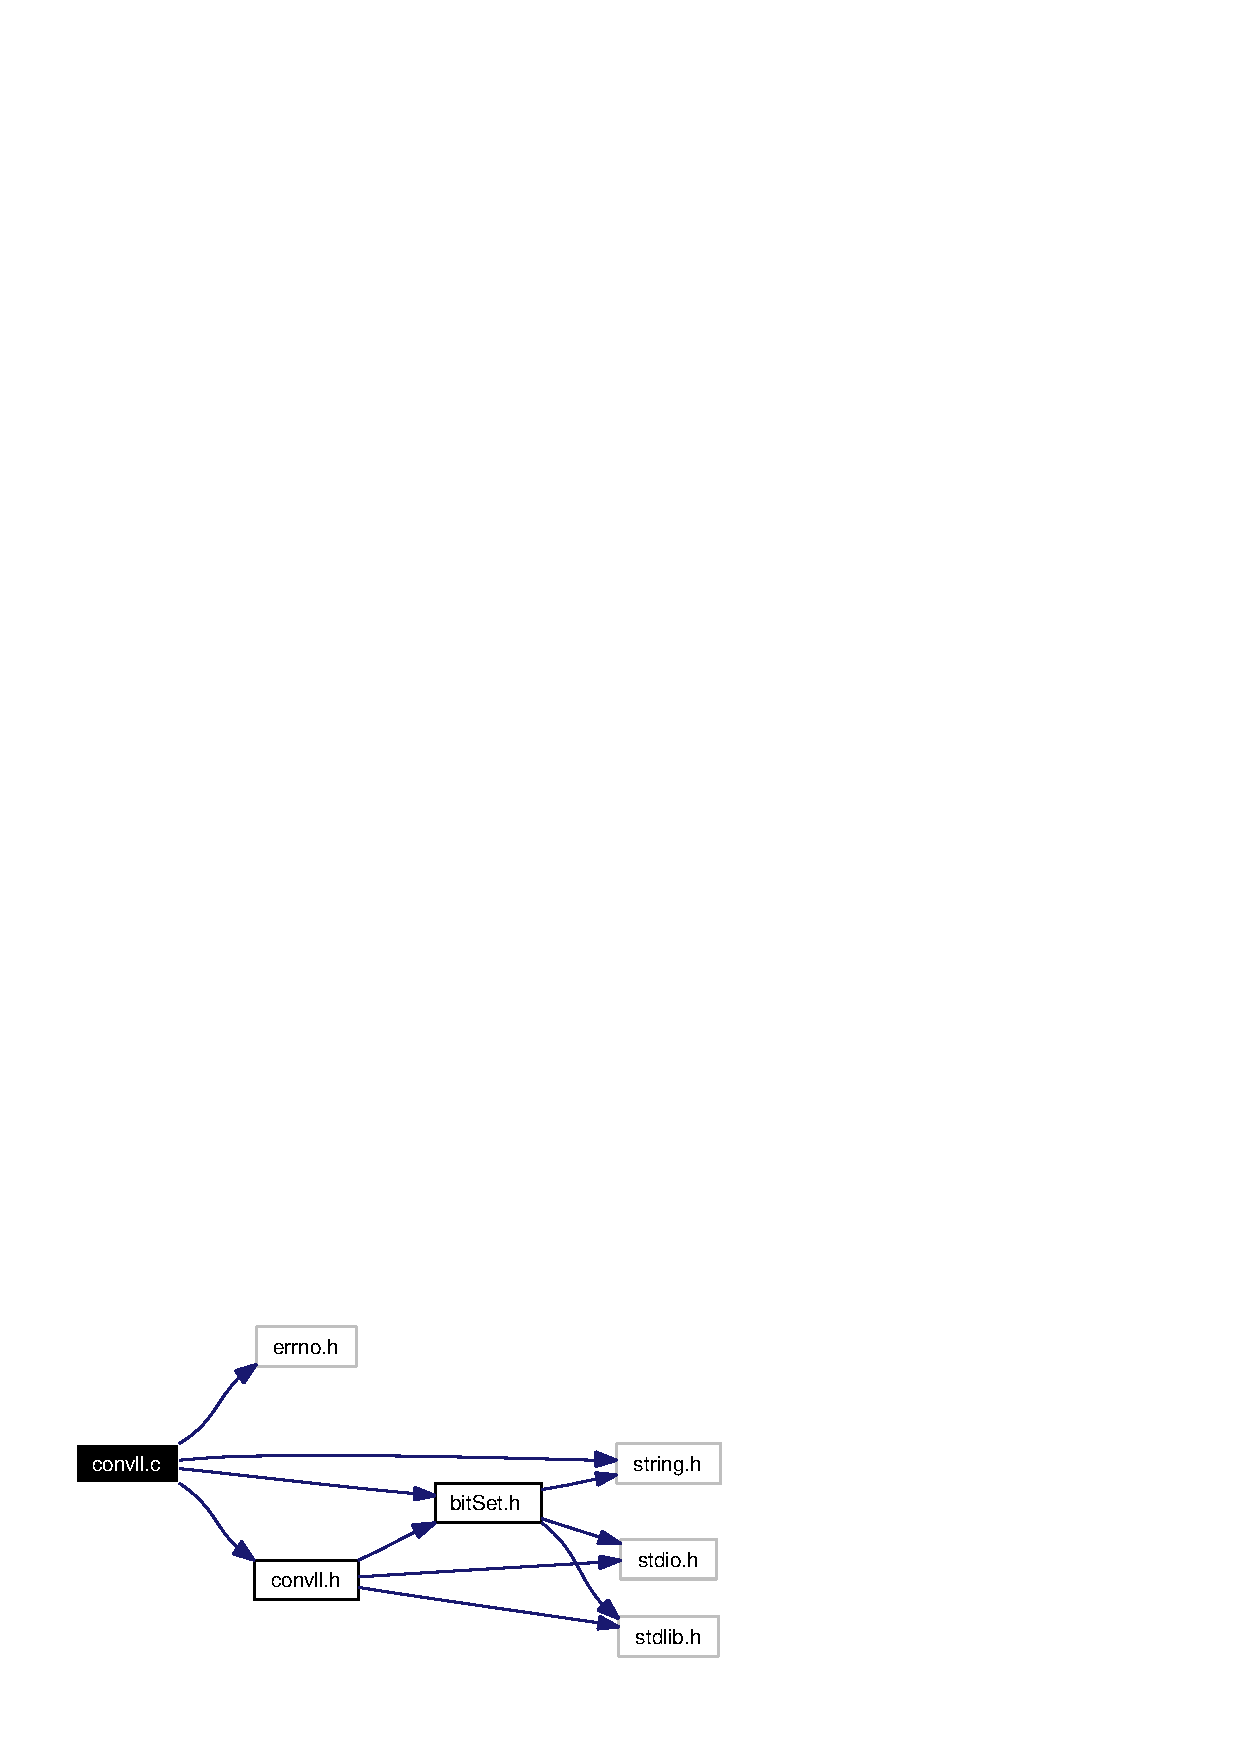
\includegraphics[width=173pt]{convll_8c__incl}
\end{center}
\end{figure}
\subsection*{Functions}
\begin{CompactItemize}
\item 
\hyperlink{structcnode}{cll\_\-t} $\ast$ \hyperlink{convll_8c_a1}{prune\-Cll} (\hyperlink{structcnode}{cll\_\-t} $\ast$head, int $\ast$index\-To\-Seq, int p)
\item 
\hyperlink{structcnode}{cll\_\-t} $\ast$ \hyperlink{convll_8c_a2}{push\-Cll} (\hyperlink{structcnode}{cll\_\-t} $\ast$head)
\item 
\hyperlink{structcnode}{cll\_\-t} $\ast$ \hyperlink{convll_8c_a3}{pop\-Cll} (\hyperlink{structcnode}{cll\_\-t} $\ast$head)
\item 
\hyperlink{structcnode}{cll\_\-t} $\ast$ \hyperlink{convll_8c_a4}{pop\-All\-Cll} (\hyperlink{structcnode}{cll\_\-t} $\ast$head)
\item 
int \hyperlink{convll_8c_a5}{print\-Cll} (\hyperlink{structcnode}{cll\_\-t} $\ast$head)
\item 
\hyperlink{structcnode}{cll\_\-t} $\ast$ \hyperlink{convll_8c_a6}{inithead\-Cll} (\hyperlink{structcnode}{cll\_\-t} $\ast$head, \hyperlink{structcSet__t}{c\-Set\_\-t} $\ast$newset)
\item 
\hyperlink{structcnode}{cll\_\-t} $\ast$ \hyperlink{convll_8c_a7}{pushc\-Set} (\hyperlink{structcnode}{cll\_\-t} $\ast$head, \hyperlink{structcSet__t}{c\-Set\_\-t} $\ast$newset)
\item 
\hyperlink{structcSet__t}{c\-Set\_\-t} $\ast$ \hyperlink{convll_8c_a8}{bit\-Set\-To\-CSet} (\hyperlink{structbitSet__t}{bit\-Set\_\-t} $\ast$clique)
\item 
int \hyperlink{convll_8c_a9}{check\-Cliquec\-Set} (\hyperlink{structcSet__t}{c\-Set\_\-t} $\ast$cliquec\-Set, int $\ast$index\-To\-Seq, int p)
\item 
\hyperlink{structcnode}{cll\_\-t} $\ast$ \hyperlink{convll_8c_a10}{push\-Clique} (\hyperlink{structbitSet__t}{bit\-Set\_\-t} $\ast$clique, \hyperlink{structcnode}{cll\_\-t} $\ast$head, int $\ast$index\-To\-Seq, int p)
\item 
\hyperlink{structmnode}{mll\_\-t} $\ast$ \hyperlink{convll_8c_a11}{push\-Mem\-Stack} (\hyperlink{structmnode}{mll\_\-t} $\ast$head, int clique\-Num)
\item 
\hyperlink{structmnode}{mll\_\-t} $\ast$ \hyperlink{convll_8c_a12}{pop\-Mem\-Stack} (\hyperlink{structmnode}{mll\_\-t} $\ast$head)
\item 
\hyperlink{structmnode}{mll\_\-t} $\ast$ \hyperlink{convll_8c_a13}{pop\-Whole\-Mem\-Stack} (\hyperlink{structmnode}{mll\_\-t} $\ast$head)
\item 
\hyperlink{structmnode}{mll\_\-t} $\ast$$\ast$ \hyperlink{convll_8c_a14}{add\-To\-Stacks} (\hyperlink{structcnode}{cll\_\-t} $\ast$node, \hyperlink{structmnode}{mll\_\-t} $\ast$$\ast$member\-Stacks)
\item 
\hyperlink{structmnode}{mll\_\-t} $\ast$$\ast$ \hyperlink{convll_8c_a15}{fill\-Member\-Stacks} (\hyperlink{structcnode}{cll\_\-t} $\ast$head, \hyperlink{structmnode}{mll\_\-t} $\ast$$\ast$member\-Stacks)
\item 
\hyperlink{structmnode}{mll\_\-t} $\ast$$\ast$ \hyperlink{convll_8c_a16}{empty\-Member\-Stacks} (\hyperlink{structmnode}{mll\_\-t} $\ast$$\ast$member\-Stacks, int size)
\item 
void \hyperlink{convll_8c_a17}{print\-Member\-Stacks} (\hyperlink{structmnode}{mll\_\-t} $\ast$$\ast$member\-Stacks, int size)
\item 
\hyperlink{structbitSet__t}{bit\-Set\_\-t} $\ast$ \hyperlink{convll_8c_a18}{set\-Stack\-True} (\hyperlink{structmnode}{mll\_\-t} $\ast$$\ast$mem\-List, int i, \hyperlink{structbitSet__t}{bit\-Set\_\-t} $\ast$queue)
\item 
\hyperlink{structbitSet__t}{bit\-Set\_\-t} $\ast$ \hyperlink{convll_8c_a19}{search\-Mems\-With\-List} (int $\ast$list, int listsize, \hyperlink{structmnode}{mll\_\-t} $\ast$$\ast$mem\-List, int num\-Offsets, \hyperlink{structbitSet__t}{bit\-Set\_\-t} $\ast$queue)
\item 
\hyperlink{structcnode}{cll\_\-t} $\ast$ \hyperlink{convll_8c_a20}{single\-Clique\-Conv} (\hyperlink{structcnode}{cll\_\-t} $\ast$head, int first\-Clique, \hyperlink{structcnode}{cll\_\-t} $\ast$$\ast$first\-Guess, int second\-Clique, \hyperlink{structcnode}{cll\_\-t} $\ast$$\ast$second\-Guess, \hyperlink{structcnode}{cll\_\-t} $\ast$next\-Phase, \hyperlink{structbitSet__t}{bit\-Set\_\-t} $\ast$print\-Status, int support)
\item 
\hyperlink{structmnode}{mll\_\-t} $\ast$ \hyperlink{convll_8c_a21}{merge\-Intersect} (\hyperlink{structcnode}{cll\_\-t} $\ast$first, \hyperlink{structcnode}{cll\_\-t} $\ast$second, \hyperlink{structmnode}{mll\_\-t} $\ast$intersection, \hyperlink{structbitSet__t}{bit\-Set\_\-t} $\ast$printstatus, int $\ast$new\-Support)
\item 
int \hyperlink{convll_8c_a22}{uniq\-Clique} (\hyperlink{structcSet__t}{c\-Set\_\-t} $\ast$cliquec\-Set, \hyperlink{structcnode}{cll\_\-t} $\ast$head)
\item 
\hyperlink{structcnode}{cll\_\-t} $\ast$ \hyperlink{convll_8c_a23}{swap\-Nodec\-Set} (\hyperlink{structcnode}{cll\_\-t} $\ast$head, int node, \hyperlink{structcSet__t}{c\-Set\_\-t} $\ast$new\-Clique)
\item 
\hyperlink{structcnode}{cll\_\-t} $\ast$ \hyperlink{convll_8c_a24}{remove\-Supers} (\hyperlink{structcnode}{cll\_\-t} $\ast$head, int node, \hyperlink{structcSet__t}{c\-Set\_\-t} $\ast$new\-Clique)
\item 
int \hyperlink{convll_8c_a25}{print\-CSet} (\hyperlink{structcSet__t}{c\-Set\_\-t} $\ast$node)
\item 
\hyperlink{structcnode}{cll\_\-t} $\ast$ \hyperlink{convll_8c_a26}{push\-Conv\-Clique} (\hyperlink{structmnode}{mll\_\-t} $\ast$clique, \hyperlink{structcnode}{cll\_\-t} $\ast$head)
\item 
\hyperlink{structcSet__t}{c\-Set\_\-t} $\ast$ \hyperlink{convll_8c_a27}{mll\-To\-CSet} (\hyperlink{structmnode}{mll\_\-t} $\ast$clique)
\item 
\hyperlink{structcnode}{cll\_\-t} $\ast$ \hyperlink{convll_8c_a28}{whole\-Clique\-Conv} (\hyperlink{structcnode}{cll\_\-t} $\ast$head, \hyperlink{structcnode}{cll\_\-t} $\ast$node, \hyperlink{structcnode}{cll\_\-t} $\ast$$\ast$first\-Guess, \hyperlink{structmnode}{mll\_\-t} $\ast$$\ast$mem\-List, int num\-Offsets, \hyperlink{structcnode}{cll\_\-t} $\ast$next\-Phase, \hyperlink{structbitSet__t}{bit\-Set\_\-t} $\ast$print\-Status, int support)
\item 
\hyperlink{structcnode}{cll\_\-t} $\ast$ \hyperlink{convll_8c_a29}{whole\-Round\-Conv} (\hyperlink{structcnode}{cll\_\-t} $\ast$$\ast$head, \hyperlink{structmnode}{mll\_\-t} $\ast$$\ast$mem\-List, int num\-Offsets, int support, int length, \hyperlink{structcnode}{cll\_\-t} $\ast$$\ast$all\-Cliques)
\item 
int \hyperlink{convll_8c_a30}{yank\-Cll} (\hyperlink{structcnode}{cll\_\-t} $\ast$$\ast$head, \hyperlink{structcnode}{cll\_\-t} $\ast$prev, \hyperlink{structcnode}{cll\_\-t} $\ast$$\ast$curr, \hyperlink{structcnode}{cll\_\-t} $\ast$$\ast$all\-Cliques, int length)
\item 
\hyperlink{structcnode}{cll\_\-t} $\ast$ \hyperlink{convll_8c_a31}{complete\-Conv} (\hyperlink{structcnode}{cll\_\-t} $\ast$$\ast$head, int support, int num\-Offsets, int min\-Length, int $\ast$index\-To\-Seq, int p)
\item 
int \hyperlink{convll_8c_a32}{print\-Cll\-Pattern} (\hyperlink{structcnode}{cll\_\-t} $\ast$node, int length)
\end{CompactItemize}
\subsection*{Variables}
\begin{CompactItemize}
\item 
int \hyperlink{convll_8c_a0}{cliquecounter} = 0
\end{CompactItemize}


\subsection*{Detailed Description}
This file defines a number of functions for handling link lists of motifs, or cliques. The functions defined in this file are called extensively during the convolution stage of the Gemoda algorithm for both the sequence based and real value based software.

Definition in file \hyperlink{convll_8c-source}{convll.c}.

\subsection*{Function Documentation}
\hypertarget{convll_8c_a14}{
\index{convll.c@{convll.c}!addToStacks@{addToStacks}}
\index{addToStacks@{addToStacks}!convll.c@{convll.c}}
\subsubsection[addToStacks]{\setlength{\rightskip}{0pt plus 5cm}\hyperlink{structmnode}{mll\_\-t}$\ast$$\ast$ add\-To\-Stacks (\hyperlink{structcnode}{cll\_\-t} $\ast$ {\em node}, \hyperlink{structmnode}{mll\_\-t} $\ast$$\ast$ {\em member\-Stacks})}}
\label{convll_8c_a14}


For one clique, it adds membership for that clique to all of its members' member stacks. Input: a specific clique in a clique linked list, an array of member stacks. Output: the array of updated member stacks.

Definition at line 482 of file convll.c.

References cnode::id, c\-Set\_\-t::members, push\-Mem\-Stack(), and cnode::set.

Referenced by fill\-Member\-Stacks().

\scriptsize\begin{verbatim}483 {
484   int i = 0;
485   int cliqueNum = 0;
486 
487   // Make sure that we don't reference NULL values
488   if (node->set != NULL)
489     {
490       // Go through each member of the clique's set
491       for (i = 0; i < node->set->size; i++)
492     {
493       // Get the member's number
494       cliqueNum = node->set->members[i];
495       // Go to that member's linked list and push
496       // on the number of the current clique
497       memberStacks[cliqueNum] =
498         pushMemStack (memberStacks[cliqueNum], node->id);
499     }
500     }
501   else
502     {
503       fprintf (stderr, "\nNULL set for clique! - addToStacks\n");
504       fflush (stderr);
505       exit (0);
506     }
507   return memberStacks;
508 }
\end{verbatim}
\normalsize 


\hypertarget{convll_8c_a8}{
\index{convll.c@{convll.c}!bitSetToCSet@{bitSetToCSet}}
\index{bitSetToCSet@{bitSetToCSet}!convll.c@{convll.c}}
\subsubsection[bitSetToCSet]{\setlength{\rightskip}{0pt plus 5cm}\hyperlink{structcSet__t}{c\-Set\_\-t}$\ast$ bit\-Set\-To\-CSet (\hyperlink{structbitSet__t}{bit\-Set\_\-t} $\ast$ {\em clique})}}
\label{convll_8c_a8}


Converts a \hyperlink{structbitSet__t}{bit\-Set\_\-t} to a \hyperlink{structcSet__t}{c\-Set\_\-t} for the purposes of pushing it onto a linked list of cliques. The \hyperlink{structbitSet__t}{bit\-Set\_\-t} data structure is used for massive comparisons during clique-finding but is unwieldy/inefficient when it is known that the structure is sparse. The \hyperlink{structcSet__t}{c\-Set\_\-t} allows for efficient comparison of sparse bit\-Set\_\-t's. Use this just before pushing a newly-discovered clique onto a clique linked list. Input: a new clique in the form of a \hyperlink{structbitSet__t}{bit\-Set\_\-t}. Output: the same clique in the form of a \hyperlink{structcSet__t}{c\-Set\_\-t}.

Definition at line 212 of file convll.c.

References count\-Set(), c\-Set\_\-t::members, next\-Bit\-Bit\-Set(), and c\-Set\_\-t::size.

Referenced by push\-Clique(), and whole\-Clique\-Conv().

\scriptsize\begin{verbatim}213 {
214   int cliqueSize = countSet (clique);
215   int i = 0, start = 0;
216   cSet_t *holder = (cSet_t *) malloc (sizeof (cSet_t));
217 
218   // Memory error checking
219   if (holder == NULL)
220     {
221       fprintf (stderr, "\nMemory Error - bitSetToCSet - [1]\n%s\n",
222            strerror (errno));
223       fflush (stderr);
224       exit (0);
225     }
226   // More memory checking
227   holder->members = (int *) malloc (cliqueSize * sizeof (int));
228   if (holder->members == NULL)
229     {
230       fprintf (stderr, "\nMemory Error - bitSetToCSet - [2]\n%s\n",
231            strerror (errno));
232       fflush (stderr);
233       exit (0);
234     }
235 
236   // For each member of the clique in the bitSet,
237   for (i = 0; i < cliqueSize; i++)
238     {
239       // Find the next one, add its location to the members array
240       holder->members[i] = nextBitBitSet (clique, start);
241       // (But check for errors... if we get to the end of the
242       // bitSet, then something is wrong)
243       if (holder->members[i] == -1)
244     {
245       fprintf (stderr, "\nClique error - not enough members\n");
246       fflush (stderr);
247       exit (0);
248     }
249       // Increment to move on in the nextBitBitSet search
250       start = holder->members[i] + 1;
251     }
252 
253   holder->size = cliqueSize;
254   return holder;
255 }
\end{verbatim}
\normalsize 


\hypertarget{convll_8c_a9}{
\index{convll.c@{convll.c}!checkCliquecSet@{checkCliquecSet}}
\index{checkCliquecSet@{checkCliquecSet}!convll.c@{convll.c}}
\subsubsection[checkCliquecSet]{\setlength{\rightskip}{0pt plus 5cm}int check\-Cliquec\-Set (\hyperlink{structcSet__t}{c\-Set\_\-t} $\ast$ {\em cliquec\-Set}, int $\ast$ {\em index\-To\-Seq}, int {\em p})}}
\label{convll_8c_a9}


Checks to enforce the -p flag (minimum number of unique input sequences in which the motif occurs). Input: a clique in the form of a \hyperlink{structcSet__t}{c\-Set\_\-t}, pointer to the index/sequence number data structure, the -p flag value. Output: An integer: 1 for success, 0 for failure.

Definition at line 266 of file convll.c.

References c\-Set\_\-t::members, and c\-Set\_\-t::size.

Referenced by push\-Clique().

\scriptsize\begin{verbatim}267 {
268   int *seqNums = NULL;
269   int thisSeq = 0, i = 0, j = 0;
270   seqNums = (int *) malloc (p * sizeof (int));
271 
272   if (seqNums == NULL)
273     {
274       fprintf (stderr, "Memory error - checkCliquecSet\n%s\n",
275            strerror (errno));
276       fflush (stderr);
277       exit (0);
278     }
279   // Initialize an array of integers of size p to sentinel values of -1
280   for (i = 0; i < p; i++)
281     {
282       seqNums[i] = -1;
283     }
284   j = 0;
285 
286   if (cliquecSet->size < 1)
287     {
288       fprintf (stderr, "\nClique of zero size! - checkCliquecSet\n");
289       fflush (stderr);
290       exit (0);
291     }
292   // Find the first sequence number.
293   seqNums[0] = indexToSeq[cliquecSet->members[0]];
294   // Iterate over the remaining size of the clique
295   for (i = 1; i < cliquecSet->size; i++)
296     {
297       // Find the next sequence number.
298       thisSeq = indexToSeq[cliquecSet->members[i]];
299       // The member list is in monotonic order, so we only need
300       // to compare the current member to the previous member to 
301       // find out if it comes from the same sequence.
302       // If it's not from the same sequence, increment the unique
303       // sequence counter (j), store the next sequence number
304       // in the array.
305       // Also check to see if we've already reached the p threshold,
306       // and if so, then bail out.
307       if (thisSeq != seqNums[j])
308     {
309       j++;
310       seqNums[j] = thisSeq;
311       if (j == p - 1)
312         {
313           break;
314         }
315     }
316     }
317 
318   // Now just see what the value of the last number in the array is;
319   // if it's the sentinel, then we didn't find instances in p 
320   // unique sequences.  If it's not the sentinel, then we've met
321   // the -p criterion.
322   if (seqNums[p - 1] == -1)
323     {
324       free (seqNums);
325       return (0);
326     }
327   else
328     {
329       free (seqNums);
330       return (1);
331     }
332 }
\end{verbatim}
\normalsize 


\hypertarget{convll_8c_a31}{
\index{convll.c@{convll.c}!completeConv@{completeConv}}
\index{completeConv@{completeConv}!convll.c@{convll.c}}
\subsubsection[completeConv]{\setlength{\rightskip}{0pt plus 5cm}\hyperlink{structcnode}{cll\_\-t}$\ast$ complete\-Conv (\hyperlink{structcnode}{cll\_\-t} $\ast$$\ast$ {\em head}, int {\em support}, int {\em num\-Offsets}, int {\em min\-Length}, int $\ast$ {\em index\-To\-Seq}, int {\em p})}}
\label{convll_8c_a31}


Performs complete convolution given the starting list of cliques. Input: a pointer to the head of the initial clique linked list, the minimum support criterion value, the number of offsets in the sequence set, the minimum length of motifs (which is the length of motifs in the initial clique linked list), the index/Sequence data structure, and the value of the -p flag to prune based on unique sequence occurrences. Output: a linked list of all maximal cliques based on the initial clique linked list.

Definition at line 1417 of file convll.c.

References empty\-Member\-Stacks(), fill\-Member\-Stacks(), pop\-All\-Cll(), prune\-Cll(), and whole\-Round\-Conv().

Referenced by convolve().

\scriptsize\begin{verbatim}1419 {
1420   int i = 0;
1421   mll_t **memList = NULL;
1422   cll_t *nextPhase = NULL;
1423   cll_t *allCliques = NULL;
1424   int length = minLength;
1425   memList = (mll_t **) malloc (numOffsets * sizeof (mll_t *));
1426   if (memList == NULL)
1427     {
1428       fprintf (stderr, "Memory error - completeConv\n%s\n", strerror (errno));
1429       fflush (stderr);
1430       exit (0);
1431     }
1432   // The number of offsets will never change, so this can be defined
1433   // now, though we will have to change what is in these arrays later.
1434   for (i = 0; i < numOffsets; i++)
1435     {
1436       memList[i] = NULL;
1437     }
1438 
1439   // NOTE: This assumes that the elemPats all meet the support criterion
1440 
1441   // So we'll do this as long as the head is non-null.. that means that 
1442   // the initial set of cliques must be non-null.  Those are then 
1443   // convolved and the linked list for the next round is set to head,
1444   // so this continues until the linked list for the "next round" at
1445   // the end of some round is null.
1446   while (*head != NULL)
1447     {
1448       // First we get the inverse information for this round: find
1449       // out which cliques each offset is a member of.
1450       memList = fillMemberStacks (*head, memList);
1451       // printf("numOffsets.bak = %d\n",numOffsets);
1452       // // Then we convolve a whole round.
1453       nextPhase =
1454     wholeRoundConv (head, memList, numOffsets, support, length,
1455             &allCliques);
1456       // Do some housekeeping.
1457       memList = emptyMemberStacks (memList, numOffsets);
1458       popAllCll (*head);
1459       // Enforce the -p flag for subsequent rounds.
1460       if (p > 1)
1461     {
1462       nextPhase = pruneCll (nextPhase, indexToSeq, p);
1463     }
1464       // And move on to the next round of convolution.
1465       *head = nextPhase;
1466       length++;
1467     }
1468 
1469   free (memList);
1470 
1471   return allCliques;
1472 }
\end{verbatim}
\normalsize 


\hypertarget{convll_8c_a16}{
\index{convll.c@{convll.c}!emptyMemberStacks@{emptyMemberStacks}}
\index{emptyMemberStacks@{emptyMemberStacks}!convll.c@{convll.c}}
\subsubsection[emptyMemberStacks]{\setlength{\rightskip}{0pt plus 5cm}\hyperlink{structmnode}{mll\_\-t}$\ast$$\ast$ empty\-Member\-Stacks (\hyperlink{structmnode}{mll\_\-t} $\ast$$\ast$ {\em member\-Stacks}, int {\em size})}}
\label{convll_8c_a16}


After we have performed a round of convolution, this \char`\"{}empties\char`\"{} the member stacks by popping all nodes off each member linked list. Input: array of member linked lists, the size of that array (total number of offsets). Output: the array of now-empty member linked lists.

Definition at line 538 of file convll.c.

References pop\-Whole\-Mem\-Stack().

Referenced by complete\-Conv().

\scriptsize\begin{verbatim}539 {
540   int i = 0;
541 
542   for (i = 0; i < size; i++)
543     {
544       memberStacks[i] = popWholeMemStack (memberStacks[i]);
545     }
546 
547   return memberStacks;
548 }
\end{verbatim}
\normalsize 


\hypertarget{convll_8c_a15}{
\index{convll.c@{convll.c}!fillMemberStacks@{fillMemberStacks}}
\index{fillMemberStacks@{fillMemberStacks}!convll.c@{convll.c}}
\subsubsection[fillMemberStacks]{\setlength{\rightskip}{0pt plus 5cm}\hyperlink{structmnode}{mll\_\-t}$\ast$$\ast$ fill\-Member\-Stacks (\hyperlink{structcnode}{cll\_\-t} $\ast$ {\em head}, \hyperlink{structmnode}{mll\_\-t} $\ast$$\ast$ {\em member\-Stacks})}}
\label{convll_8c_a15}


Fills the entire member\-Stacks data structure by calling add\-To\-Stacks for each clique in the clique linked list. Input: head of a clique linked list, array of member linked lists. Output: the array of updated member linked lists.

Definition at line 517 of file convll.c.

References add\-To\-Stacks(), and cnode::next.

Referenced by complete\-Conv().

\scriptsize\begin{verbatim}518 {
519   cll_t *curr = head;
520   // Just go down the linked list calling addToStacks
521   while (curr != NULL)
522     {
523       memberStacks = addToStacks (curr, memberStacks);
524       curr = curr->next;
525     }
526 
527   return memberStacks;
528 }
\end{verbatim}
\normalsize 


\hypertarget{convll_8c_a6}{
\index{convll.c@{convll.c}!initheadCll@{initheadCll}}
\index{initheadCll@{initheadCll}!convll.c@{convll.c}}
\subsubsection[initheadCll]{\setlength{\rightskip}{0pt plus 5cm}\hyperlink{structcnode}{cll\_\-t}$\ast$ inithead\-Cll (\hyperlink{structcnode}{cll\_\-t} $\ast$ {\em head}, \hyperlink{structcSet__t}{c\-Set\_\-t} $\ast$ {\em newset})}}
\label{convll_8c_a6}


Initializes the empty head of a linked list by adding a set to that head. Note: this is only called immediately after pushing onto a cll, because the push always creates a new empty head. This function should not be called by the user; see pushc\-Set. Input: head of a linked list, pointer to a \hyperlink{structcSet__t}{c\-Set\_\-t} list of clique members. Output: head of a linked list.

Definition at line 172 of file convll.c.

References cnode::set.

Referenced by pushc\-Set().

\scriptsize\begin{verbatim}173 {
174   // Check to make sure that the head is not already initialized.
175   if (head->set != NULL)
176     {
177       printf ("Stack head already initialized!");
178       exit (0);
179     }
180   // Make the head's set pointer point to the new set.
181   head->set = newset;
182   return head;
183 }
\end{verbatim}
\normalsize 


\hypertarget{convll_8c_a21}{
\index{convll.c@{convll.c}!mergeIntersect@{mergeIntersect}}
\index{mergeIntersect@{mergeIntersect}!convll.c@{convll.c}}
\subsubsection[mergeIntersect]{\setlength{\rightskip}{0pt plus 5cm}\hyperlink{structmnode}{mll\_\-t}$\ast$ merge\-Intersect (\hyperlink{structcnode}{cll\_\-t} $\ast$ {\em first}, \hyperlink{structcnode}{cll\_\-t} $\ast$ {\em second}, \hyperlink{structmnode}{mll\_\-t} $\ast$ {\em intersection}, \hyperlink{structbitSet__t}{bit\-Set\_\-t} $\ast$ {\em printstatus}, int $\ast$ {\em new\-Support})}}
\label{convll_8c_a21}


Convolves two cliques in a non-commutative manner. It finds which members of the first clique are immediately followed by a member in the second clique. Input: pointer to the location in the linked list of the first clique to be convolved, pointer to the location in the linked list of the second clique to be convolved, a member linked list used to store the intersection of the two cliques, the printstatus bit\-Set, and a pointer to an integer with the support of the clique formed by convolution. Output: a member linked list with the intersection of the two cliques, plus the side effect of that intersection's cardinality being stored in the integer pointed to by new\-Support.

Definition at line 759 of file convll.c.

References c\-Set\_\-t::members, push\-Mem\-Stack(), and cnode::set.

Referenced by single\-Clique\-Conv().

\scriptsize\begin{verbatim}761 {
762 
763   int i = 0, j = 0, status = 0;
764 
765   // Make sure we are still in-bounds, otherwise we bail out
766   // We'll refer to the offset currently being analyzed from the 
767   // first clique as the 'first offset' and the offset currently
768   // being analyzed from the second clique as the 'second offset'
769   while ((i < first->set->size) && (j < second->set->size))
770     {
771       // If the second offset is earlier than the first offset plus
772       // one, then we move on to the next possible second offset
773       if ((first->set->members[i] + 1) > second->set->members[j])
774     {
775       j++;
776     }
777       // If the second offset is later than the first offset plus
778       // one, then we move on the next possible first offset
779       else if ((first->set->members[i] + 1) < second->set->members[j])
780     {
781       i++;
782     }
783       // Otherwise, the second offset is equal to the first offset
784       // plus one, so we have an extendable node.  Push that on
785       // to the intersection stack, move both the first and second
786       // offsets to their respective next possible offsets, and 
787       // increment the support counter for the new clique (status)
788       else
789     {
790       intersection = pushMemStack (intersection, first->set->members[i]);
791       i++;
792       j++;
793       status++;
794     }
795     }
796 
797   // Send the value of the clique's new support out of this function
798   *newSupport = status;
799   return intersection;
800 }
\end{verbatim}
\normalsize 


\hypertarget{convll_8c_a27}{
\index{convll.c@{convll.c}!mllToCSet@{mllToCSet}}
\index{mllToCSet@{mllToCSet}!convll.c@{convll.c}}
\subsubsection[mllToCSet]{\setlength{\rightskip}{0pt plus 5cm}\hyperlink{structcSet__t}{c\-Set\_\-t}$\ast$ mll\-To\-CSet (\hyperlink{structmnode}{mll\_\-t} $\ast$ {\em clique})}}
\label{convll_8c_a27}


Turns a member linked list used to store the intersection of two cliques into something more useful: a \hyperlink{structcSet__t}{c\-Set\_\-t} structure. Input: a clique in mll\_\-t form. Output: a clique in \hyperlink{structcSet__t}{c\-Set\_\-t} form.

Definition at line 1145 of file convll.c.

References mnode::clique\-Membership, c\-Set\_\-t::members, mnode::next, and c\-Set\_\-t::size.

Referenced by push\-Conv\-Clique().

\scriptsize\begin{verbatim}1146 {
1147   int sizecount = 0, i = 0;
1148   cSet_t *cliqueCset = malloc (sizeof (cSet_t));
1149   mll_t *head = clique;
1150   if (cliqueCset == NULL)
1151     {
1152       fprintf (stderr, "Memory error - mllToCSet cSet\n%s\n",
1153            strerror (errno));
1154       fflush (stderr);
1155       exit (0);
1156     }
1157   // First count up how many members there are in the member linked list
1158   while (head != NULL)
1159     {
1160       sizecount++;
1161       head = head->next;
1162     }
1163 
1164   head = clique;
1165   cliqueCset->size = sizecount;
1166   cliqueCset->members = (int *) malloc (sizecount * sizeof (int));
1167 
1168   if (cliqueCset->members == NULL)
1169     {
1170       fprintf (stderr, "Memory error - mllTlCSet cliquemembers\n%s\n",
1171            strerror (errno));
1172       fflush (stderr);
1173       exit (0);
1174     }
1175   // In order to stay in the same format as with bitSet translation to
1176   // cSet, we ensure that the ids of the members are ascending with
1177   // ascending index number in the cSet.  This is accomplished by noting
1178   // that since the intersection members are pushed onto the stack,
1179   // a LIFO operation, that the first intersected nodes off the stack
1180   // will have the highest ids, so we will put them at the end of
1181   // the members array with the higher index values.
1182   for (i = sizecount - 1; i >= 0; i--)
1183     {
1184       cliqueCset->members[i] = head->cliqueMembership;
1185       head = head->next;
1186     }
1187 
1188   return cliqueCset;
1189 }
\end{verbatim}
\normalsize 


\hypertarget{convll_8c_a4}{
\index{convll.c@{convll.c}!popAllCll@{popAllCll}}
\index{popAllCll@{popAllCll}!convll.c@{convll.c}}
\subsubsection[popAllCll]{\setlength{\rightskip}{0pt plus 5cm}\hyperlink{structcnode}{cll\_\-t}$\ast$ pop\-All\-Cll (\hyperlink{structcnode}{cll\_\-t} $\ast$ {\em head})}}
\label{convll_8c_a4}


Shortcut function to pop all of the members of a linked list. Input: head of a linked list. Output: head of a now-empty linked list.

Definition at line 109 of file convll.c.

References pop\-Cll().

Referenced by complete\-Conv(), and main().

\scriptsize\begin{verbatim}110 {
111   while (head != NULL)
112     {
113       head = popCll (head);
114     }
115   return head;
116 }
\end{verbatim}
\normalsize 


\hypertarget{convll_8c_a3}{
\index{convll.c@{convll.c}!popCll@{popCll}}
\index{popCll@{popCll}!convll.c@{convll.c}}
\subsubsection[popCll]{\setlength{\rightskip}{0pt plus 5cm}\hyperlink{structcnode}{cll\_\-t}$\ast$ pop\-Cll (\hyperlink{structcnode}{cll\_\-t} $\ast$ {\em head})}}
\label{convll_8c_a3}


Removes the head of the clique linked list, returns the new head of the clique linked list, and frees the memory occupied by the old head. Input: head of a linked list. Output: head of a linked list.

Definition at line 66 of file convll.c.

References c\-Set\_\-t::members, cnode::next, and cnode::set.

Referenced by pop\-All\-Cll().

\scriptsize\begin{verbatim}67 {
68   // by default the new head is NULL...is important later
69   cll_t *newHead = NULL;
70   if (head == NULL)
71     {
72       fprintf (stderr, "\nCan't pop a null linked list\n");
73       fflush (stderr);
74       exit (0);
75     }
76   // unless this is the end of the linked list, set the new head
77   // to the next member of the list.  Otherwise, since by default the
78   // new head is NULL, it will properly return an empty list
79   if (head->next != NULL)
80     {
81       newHead = head->next;
82     }
83   // Check to see if there is a set.  If there is, and there are members,
84   // then first free the members.  And if there is a set, then free it.
85   if (head->set != NULL)
86     {
87       if (head->set->members != NULL)
88     {
89       free (head->set->members);
90       head->set->members = NULL;
91     }
92       free (head->set);
93       head->set = NULL;
94     }
95   // Both the members and set have been freed, so now can free the cll_t
96   // without leaking anything.
97 
98   free (head);
99   head = NULL;
100   return newHead;
101 }
\end{verbatim}
\normalsize 


\hypertarget{convll_8c_a12}{
\index{convll.c@{convll.c}!popMemStack@{popMemStack}}
\index{popMemStack@{popMemStack}!convll.c@{convll.c}}
\subsubsection[popMemStack]{\setlength{\rightskip}{0pt plus 5cm}\hyperlink{structmnode}{mll\_\-t}$\ast$ pop\-Mem\-Stack (\hyperlink{structmnode}{mll\_\-t} $\ast$ {\em head})}}
\label{convll_8c_a12}


Pops the head off of a single member linked list. Input: head of a member linked list. Output: the new head of a member linked list after popping one item.

Definition at line 440 of file convll.c.

References mnode::next.

Referenced by pop\-Whole\-Mem\-Stack().

\scriptsize\begin{verbatim}441 {
442   // by default the new head is NULL...is important later
443   mll_t *newHead = NULL;
444   if (head == NULL)
445     {
446       fprintf (stderr, "\nCan't pop a null linked list - popMemStack\n");
447       fflush (stderr);
448       exit (0);
449     }
450   if (head->next != NULL)
451     {
452       newHead = head->next;
453     }
454   free (head);
455   head = NULL;
456   return newHead;
457 }
\end{verbatim}
\normalsize 


\hypertarget{convll_8c_a13}{
\index{convll.c@{convll.c}!popWholeMemStack@{popWholeMemStack}}
\index{popWholeMemStack@{popWholeMemStack}!convll.c@{convll.c}}
\subsubsection[popWholeMemStack]{\setlength{\rightskip}{0pt plus 5cm}\hyperlink{structmnode}{mll\_\-t}$\ast$ pop\-Whole\-Mem\-Stack (\hyperlink{structmnode}{mll\_\-t} $\ast$ {\em head})}}
\label{convll_8c_a13}


Pops all items off of a member linked list. Input: head of a member linked list. Output: empty head of a member linked list.

Definition at line 465 of file convll.c.

References pop\-Mem\-Stack().

Referenced by empty\-Member\-Stacks(), and single\-Clique\-Conv().

\scriptsize\begin{verbatim}466 {
467   while (head != NULL)
468     {
469       head = popMemStack (head);
470     }
471   return head;
472 }
\end{verbatim}
\normalsize 


\hypertarget{convll_8c_a5}{
\index{convll.c@{convll.c}!printCll@{printCll}}
\index{printCll@{printCll}!convll.c@{convll.c}}
\subsubsection[printCll]{\setlength{\rightskip}{0pt plus 5cm}int print\-Cll (\hyperlink{structcnode}{cll\_\-t} $\ast$ {\em head})}}
\label{convll_8c_a5}


Prints the members (cliques) of a linked list in the format: {\em id\/} = unique id number of clique within linked list; {\em Length\/} = number of members of clique, if available; {\em Size\/} = length of each member of clique; {\em Members\/} = newline-separated list of members of the clique. Input: head of a linked list. Output: Gives text output, returns (meaningless) exit value.

Definition at line 128 of file convll.c.

References cnode::id, cnode::length, c\-Set\_\-t::members, cnode::next, cnode::set, and c\-Set\_\-t::size.

\scriptsize\begin{verbatim}129 {
130   int i = 0;
131   cll_t *curr = head;
132   while (curr != NULL)
133     {
134       printf ("id = %d\n", curr->id);
135       // Make sure the clique is nonzero in size before attempting
136       // to print it
137       if ((curr->set != NULL) && (curr->set->size > 0))
138     {
139       if (curr->length >= 0)
140         {
141           printf ("Length = %d\n", curr->length);
142         }
143       printf ("Size = %d\n", curr->set->size);
144       printf ("Members = \n");
145       for (i = 0; i < curr->set->size; i++)
146         {
147           printf ("\t%d\n", curr->set->members[i]);
148         }
149       printf ("***********************************************\n");
150     }
151       else
152     {
153       fprintf (stderr, "\nClique has no members! -- printCll\n");
154       fflush (stderr);
155       exit (0);
156     }
157       curr = curr->next;
158     }
159   return EXIT_SUCCESS;
160 }
\end{verbatim}
\normalsize 


\hypertarget{convll_8c_a32}{
\index{convll.c@{convll.c}!printCllPattern@{printCllPattern}}
\index{printCllPattern@{printCllPattern}!convll.c@{convll.c}}
\subsubsection[printCllPattern]{\setlength{\rightskip}{0pt plus 5cm}int print\-Cll\-Pattern (\hyperlink{structcnode}{cll\_\-t} $\ast$ {\em node}, int {\em length})}}
\label{convll_8c_a32}


Prints out the contents of a clique linked list node in this format: {\em support\/} = number of motif occurrences ({\em id\/} = some id number); {\em members\/} = newline-separated list of offsets. Input: a specific node to be output, the length of the motif inside it. Output: text per above, and an integer success value.

Definition at line 1482 of file convll.c.

References cnode::id, c\-Set\_\-t::members, cnode::set, and c\-Set\_\-t::size.

\scriptsize\begin{verbatim}1483 {
1484   int i = 0;
1485 
1486   printf ("\nSupport = %d\t(id = %d)\n", node->set->size, node->id);
1487   printf ("Members = \n");
1488   for (i = 0; i < node->set->size; i++)
1489     {
1490       printf ("\t%d\n", node->set->members[i]);
1491     }
1492   return 1;
1493 }
\end{verbatim}
\normalsize 


\hypertarget{convll_8c_a25}{
\index{convll.c@{convll.c}!printCSet@{printCSet}}
\index{printCSet@{printCSet}!convll.c@{convll.c}}
\subsubsection[printCSet]{\setlength{\rightskip}{0pt plus 5cm}int print\-CSet (\hyperlink{structcSet__t}{c\-Set\_\-t} $\ast$ {\em node})}}
\label{convll_8c_a25}


Prints out the contents of a \hyperlink{structcSet__t}{c\-Set\_\-t} in the following format: {\em support\/} = number of nodes in clique; {\em members\/} = newline-separated list of nodes in clique. Input: a clique in the form of a \hyperlink{structcSet__t}{c\-Set\_\-t} object. Output: in text, the contents of the \hyperlink{structcSet__t}{c\-Set\_\-t} object. An integer is returned as well, with 1 indicating success.

Definition at line 1068 of file convll.c.

References c\-Set\_\-t::members, and c\-Set\_\-t::size.

\scriptsize\begin{verbatim}1069 {
1070   int i = 0;
1071   if (node->size == 0)
1072     {
1073       fprintf (stderr, "cSet has no members! - printCSet\n");
1074       fflush (stderr);
1075       exit (0);
1076     }
1077   else
1078     {
1079       printf ("\nSupport = %d\n", node->size);
1080       printf ("Members = \n");
1081       for (i = 0; i < node->size; i++)
1082     {
1083       printf ("\t%d\n", node->members[i]);
1084     }
1085       return 1;
1086     }
1087 }
\end{verbatim}
\normalsize 


\hypertarget{convll_8c_a17}{
\index{convll.c@{convll.c}!printMemberStacks@{printMemberStacks}}
\index{printMemberStacks@{printMemberStacks}!convll.c@{convll.c}}
\subsubsection[printMemberStacks]{\setlength{\rightskip}{0pt plus 5cm}void print\-Member\-Stacks (\hyperlink{structmnode}{mll\_\-t} $\ast$$\ast$ {\em member\-Stacks}, int {\em size})}}
\label{convll_8c_a17}


Prints the contents of the member stacks. Input: array of member linked lists, size of that array (total number of offsets). Output: only text output/no return value.

Definition at line 557 of file convll.c.

References mnode::clique\-Membership, and mnode::next.

\scriptsize\begin{verbatim}558 {
559   int i = 0;
560   mll_t *curr = NULL;
561 
562   for (i = 0; i < size; i++)
563     {
564       curr = memberStacks[i];
565       printf ("Offset %d: ", i);
566       while (curr != NULL)
567     {
568       printf ("%d,", curr->cliqueMembership);
569       curr = curr->next;
570     }
571       printf ("\n");
572     }
573 }
\end{verbatim}
\normalsize 


\hypertarget{convll_8c_a1}{
\index{convll.c@{convll.c}!pruneCll@{pruneCll}}
\index{pruneCll@{pruneCll}!convll.c@{convll.c}}
\subsubsection[pruneCll]{\setlength{\rightskip}{0pt plus 5cm}\hyperlink{structcnode}{cll\_\-t}$\ast$ prune\-Cll (\hyperlink{structcnode}{cll\_\-t} $\ast$ {\em head}, int $\ast$ {\em index\-To\-Seq}, int {\em p})}}
\label{convll_8c_a1}


Prunes a motif linked list of all motifs without support in at least

unique source sequences. Input: head of a motif linked list, pointer to a structure that dereferences offset indices to sequence numbers, minimum number of unique source sequences in which a motif must occur. Output: head of a (potentially altered) motif linked list.

Definition at line 514 of file new\-Conv.c.

References c\-Set\_\-t::members, cnode::next, cnode::set, and c\-Set\_\-t::size.

Referenced by complete\-Conv(), and convolve().

\scriptsize\begin{verbatim}515 {
516   int i = 0, j = 0, thisSeq = 0;
517   int *seqNums = NULL;
518   cll_t * curr = head;
519   cll_t * prev = NULL;
520   cll_t * storage = NULL;
521   
522     // We'll do this similar to the pruneBitGraph function... we will
523     // keep track of which source sequence each motif occurrence was in.
524     // Again, since the occurrences are listed monotonically, we only
525     // need to compare the last non-sentinel index to the current
526     // sequence number.
527     seqNums = (int *) malloc (p * sizeof (int));
528   if (seqNums == NULL)
529     {
530       fprintf (stderr, "Memory error - pruneCll\n%s\n", strerror (errno));
531       fflush (stderr);
532       exit (0);
533     }
534   while (curr != NULL)
535     {
536       
537     // First make sure the set size is at least p.
538     // This is redundant, but extremely simple and not expensive,
539     // so we'll leave it in just as a check.
540     if (curr->set->size < p)
541     {
542       if (prev != NULL)
543         {
544           prev->next = curr->next;
545         }
546       else
547         {
548           head = curr->next;
549         }
550       storage = curr->next;
551       free (curr->set->members);
552       free (curr->set);
553       free (curr);
554       curr = storage;
555       continue;
556     }
557       for (i = 0; i < p; i++)
558     {
559       seqNums[i] = -1;
560     }
561       j = 0;
562       seqNums[0] = indexToSeq[curr->set->members[0]];
563       
564     // Note, we've checked to make sure size > p, and we know
565     // p must be 2 or greater, so we can start at 1 without
566     // worrying about segfaulting
567     for (i = 1; i < curr->set->size; i++)
568     {
569       thisSeq = indexToSeq[curr->set->members[i]];
570       if (thisSeq != seqNums[j])
571         {
572           j++;
573           seqNums[j] = thisSeq;
574           if (j == p - 1)
575         {
576           break;
577         }
578         }
579     }
580       
581     // Same story as before... if the last number is -1,
582     // then we didn't have enough to fill up the <p> different
583     // slots, so this doesn't meet our criterion.
584     if (seqNums[p - 1] == -1)
585     {
586       if (prev != NULL)
587         {
588           prev->next = curr->next;
589         }
590       else
591         {
592           head = curr->next;
593         }
594       storage = curr->next;
595       free (curr->set->members);
596       free (curr->set);
597       free (curr);
598       curr = storage;
599     }
600       else
601     {
602       prev = curr;
603       curr = curr->next;
604     }
605     }
606   free (seqNums);
607   return (head);
608 }
\end{verbatim}
\normalsize 


\hypertarget{convll_8c_a10}{
\index{convll.c@{convll.c}!pushClique@{pushClique}}
\index{pushClique@{pushClique}!convll.c@{convll.c}}
\subsubsection[pushClique]{\setlength{\rightskip}{0pt plus 5cm}\hyperlink{structcnode}{cll\_\-t}$\ast$ push\-Clique (\hyperlink{structbitSet__t}{bit\-Set\_\-t} $\ast$ {\em clique}, \hyperlink{structcnode}{cll\_\-t} $\ast$ {\em head}, int $\ast$ {\em index\-To\-Seq}, int {\em p})}}
\label{convll_8c_a10}


Pushes a bit\-Set onto a clique linked list, performing all necessary manipulations in order to do so. Input: new clique in the form of a \hyperlink{structbitSet__t}{bit\-Set\_\-t}, head of a linked list, pointer to the index/sequence number data structure, integer value of the -p flag. Output: head of an updated clique linked list.

Definition at line 345 of file convll.c.

References bit\-Set\-To\-CSet(), check\-Cliquec\-Set(), cliquecounter, and pushc\-Set().

Referenced by find\-Cliques(), and single\-Linkage().

\scriptsize\begin{verbatim}346 {
347   cSet_t *cliquecSet = NULL;
348 
349   // Change the bitSet_t to a cSet_t
350   cliquecSet = bitSetToCSet (clique);
351   // If the -p flag has been assigned a value, then check the clique
352   // and only proceed if that criterion is met.  Otherwise, free the
353   // memory that we had allocated up to this point.
354   if (p > 1)
355     {
356       if (checkCliquecSet (cliquecSet, indexToSeq, p))
357     {
358       cliquecounter++;
359       /*
360          printf("%d\n",cliquecounter);
361        */
362       /*
363          fflush(stdout);
364        */
365       head = pushcSet (head, cliquecSet);
366     }
367       else
368     {
369       free (cliquecSet->members);
370       free (cliquecSet);
371     }
372       // If the -p flag wasn't set, then just push the cSet onto the linked
373       // list.
374     }
375   else
376     {
377       cliquecounter++;
378       /*
379          printf("%d\n",cliquecounter);
380        */
381       /*
382          fflush(stdout);
383        */
384       head = pushcSet (head, cliquecSet);
385     }
386   return head;
387 }
\end{verbatim}
\normalsize 


\hypertarget{convll_8c_a2}{
\index{convll.c@{convll.c}!pushCll@{pushCll}}
\index{pushCll@{pushCll}!convll.c@{convll.c}}
\subsubsection[pushCll]{\setlength{\rightskip}{0pt plus 5cm}\hyperlink{structcnode}{cll\_\-t}$\ast$ push\-Cll (\hyperlink{structcnode}{cll\_\-t} $\ast$ {\em head})}}
\label{convll_8c_a2}


Pushes a new, empty head onto a linked list of cliques. Note: this should always be followed by a call to inithead\-Cll, as the head pushed on here is empty and will be meaningless without any members. This function should NOT be used by the user; see pushc\-Set. Input: head of a linked list. Output: head of a linked list.

Definition at line 28 of file convll.c.

References cnode::id, cnode::length, cnode::next, cnode::set, and cnode::stat.

Referenced by pushc\-Set().

\scriptsize\begin{verbatim}29 {
30   // Make a pointer, verify memory
31   cll_t *a = NULL;
32   a = (cll_t *) malloc (sizeof (cll_t));
33   if (a == NULL)
34     {
35       fprintf (stderr, "\nMemory Error - pushCll\n%s\n", strerror (errno));
36       fflush (stderr);
37       exit (0);
38     }
39   // Initialize id (sequential) and pointer to next item, but not
40   // the cSet with the clique members
41   if (head == NULL)
42     {
43       a->id = 0;
44       a->next = NULL;
45     }
46   else
47     {
48       a->next = head;
49       a->id = head->id + 1;
50     }
51   a->set = NULL;
52   a->length = -1;
53   a->stat = -1;
54   return a;
55 }
\end{verbatim}
\normalsize 


\hypertarget{convll_8c_a26}{
\index{convll.c@{convll.c}!pushConvClique@{pushConvClique}}
\index{pushConvClique@{pushConvClique}!convll.c@{convll.c}}
\subsubsection[pushConvClique]{\setlength{\rightskip}{0pt plus 5cm}\hyperlink{structcnode}{cll\_\-t}$\ast$ push\-Conv\-Clique (\hyperlink{structmnode}{mll\_\-t} $\ast$ {\em clique}, \hyperlink{structcnode}{cll\_\-t} $\ast$ {\em head})}}
\label{convll_8c_a26}


Pushes a freshly-convolved clique, currently in mll\_\-t form, onto the clique linked list for the next level. Also checks to make sure that the convolved clique is unique, and if it isn't, it takes appropriate action. Input: a convolved clique in mll\_\-t form, the head of a clique linked list for the next level. Output: (potentially new) head of the clique linked list for the next level.

Definition at line 1099 of file convll.c.

References c\-Set\_\-t::members, mll\-To\-CSet(), pushc\-Set(), remove\-Supers(), swap\-Nodec\-Set(), and uniq\-Clique().

Referenced by single\-Clique\-Conv().

\scriptsize\begin{verbatim}1100 {
1101   int status = 0;
1102   cSet_t *cliquecSet = NULL;
1103 
1104   // First change the clique to something we can used more easily
1105   cliquecSet = mllToCSet (clique);
1106   // Then check to make sure it's unique by finding out its status
1107   status = uniqClique (cliquecSet, head);
1108 
1109   // printf("Candidate:\n");
1110   // printCSet(cliquecSet);
1111 
1112   // If we get -2, then this clique is a subset, so just free 
1113   // the cSet we just made and move on.
1114   if (status == -2)
1115     {
1116       free (cliquecSet->members);
1117       free (cliquecSet);
1118       cliquecSet = NULL;
1119     }
1120   // If we get -1, then this is a unique clique, so push it on.
1121   else if (status == -1)
1122     {
1123       head = pushcSet (head, cliquecSet);
1124     }
1125   // Otherwise, this clique is a superset, so we'll first remove
1126   // all of the other cliques of which this is a superset.  Then
1127   // we'll swap out the first clique of which this is a superset
1128   // with this current clique.  The clique being removed is free'd 
1129   // within the swapNode function.
1130   else
1131     {
1132       head = removeSupers (head, status, cliquecSet);
1133       head = swapNodecSet (head, status, cliquecSet);
1134     }
1135   return head;
1136 }
\end{verbatim}
\normalsize 


\hypertarget{convll_8c_a7}{
\index{convll.c@{convll.c}!pushcSet@{pushcSet}}
\index{pushcSet@{pushcSet}!convll.c@{convll.c}}
\subsubsection[pushcSet]{\setlength{\rightskip}{0pt plus 5cm}\hyperlink{structcnode}{cll\_\-t}$\ast$ pushc\-Set (\hyperlink{structcnode}{cll\_\-t} $\ast$ {\em head}, \hyperlink{structcSet__t}{c\-Set\_\-t} $\ast$ {\em newset})}}
\label{convll_8c_a7}


Function that pushes the contents of a c\-Set (set of members of a clique) onto a linked list of cliques. Input: head of a linked list, new clique in the form of a \hyperlink{structcSet__t}{c\-Set\_\-t}. Output: head of a linked list.

Definition at line 192 of file convll.c.

References inithead\-Cll(), and push\-Cll().

Referenced by push\-Clique(), and push\-Conv\-Clique().

\scriptsize\begin{verbatim}193 {
194   head = pushCll (head);
195   head = initheadCll (head, newset);
196   return head;
197 }
\end{verbatim}
\normalsize 


\hypertarget{convll_8c_a11}{
\index{convll.c@{convll.c}!pushMemStack@{pushMemStack}}
\index{pushMemStack@{pushMemStack}!convll.c@{convll.c}}
\subsubsection[pushMemStack]{\setlength{\rightskip}{0pt plus 5cm}\hyperlink{structmnode}{mll\_\-t}$\ast$ push\-Mem\-Stack (\hyperlink{structmnode}{mll\_\-t} $\ast$ {\em head}, int {\em clique\-Num})}}
\label{convll_8c_a11}


This begins code for the member linked lists. A single one of these linked lists functions somewhat similarly to the clique linked lists, though with less information stored. Functionally, an array of member linked lists is used to access the \char`\"{}inverse\char`\"{} of what is contained in the clique linked lists. That is, we would like to be able to look up the cliques that a given node is a member of, so we have an array of member linked lists of size equal to the number of nodes.

This function pushes a single clique membership onto a node's member stack. Input: the head of a single member linked list, a clique number to be added. Output: the head of a single member linked list.

Definition at line 404 of file convll.c.

References mnode::clique\-Membership, and mnode::next.

Referenced by add\-To\-Stacks(), and merge\-Intersect().

\scriptsize\begin{verbatim}405 {
406   mll_t *a = NULL;
407   a = (mll_t *) malloc (sizeof (mll_t));
408   // Memory error checking
409   if (a == NULL)
410     {
411       fprintf (stderr, "\nMemory Error - pushMemStack: %s\n",
412            strerror (errno));
413       fflush (stderr);
414       exit (0);
415     }
416   if (head == NULL)
417     {
418       a->next = NULL;
419     }
420   else
421     {
422       a->next = head;
423     }
424   // Store the number of the clique of which the node is a member.
425   // Note that we assume no duplication, which is guaranteed
426   // by our method of filling the member stacks, which is quite simple:
427   // go through all members of a clique (which have no duplicates
428   // because they are constructed from merge-intersections or from
429   // bitSet_t's) and add that clique to each node's membership list.
430   a->cliqueMembership = cliqueNum;
431   return a;
432 }
\end{verbatim}
\normalsize 


\hypertarget{convll_8c_a24}{
\index{convll.c@{convll.c}!removeSupers@{removeSupers}}
\index{removeSupers@{removeSupers}!convll.c@{convll.c}}
\subsubsection[removeSupers]{\setlength{\rightskip}{0pt plus 5cm}\hyperlink{structcnode}{cll\_\-t}$\ast$ remove\-Supers (\hyperlink{structcnode}{cll\_\-t} $\ast$ {\em head}, int {\em node}, \hyperlink{structcSet__t}{c\-Set\_\-t} $\ast$ {\em new\-Clique})}}
\label{convll_8c_a24}


This function finds all cliques in a linked list of which the proposed clique is a superset. It starts looking AFTER the first clique which has already been found to be a subset. In some senses, it is just a continuation of the uniqclique function in order to take advantage of the fact that though a proposed clique can only be a subset of one existing next-level clique, it can be a superset of many existing next- level cliques. Input: head of a clique linked list, the id of the first node found to be a subset of the proposed clique, and the proposed clique (in \hyperlink{structcSet__t}{c\-Set\_\-t} form). Output: the head of the clique linked list with all but the first subset (which was passed as an argument) removed. This function is now ready for swap\-Node to be called.

Definition at line 952 of file convll.c.

References cnode::id, c\-Set\_\-t::members, cnode::next, cnode::set, and c\-Set\_\-t::size.

Referenced by push\-Conv\-Clique().

\scriptsize\begin{verbatim}953 {
954   int foundStatus = 0;
955   cll_t *curr = head;
956   cll_t *prev = NULL;
957   int i = 0, j = 0, breakFlag = 0;
958 
959   while (curr != NULL)
960     {
961       if (curr->id == node)
962     {
963       foundStatus = 1;
964       break;
965     }
966       curr = curr->next;
967     }
968 
969   if (foundStatus == 0)
970     {
971       fprintf (stderr, "\nFirst clique not found! (removeSupers)\n");
972       fflush (stderr);
973       exit (0);
974     }
975   // Now this is trickier, to remove nodes from the middle of a linked
976   // list; this means that we need to remember which node we were just
977   // at so that we can connect it to the node after the one we are 
978   // about to delete.
979   prev = curr;
980   curr = curr->next;
981 
982   // This code is similar to that in uniqClique.
983   // Descend through all members of the next level's linked list.
984   while (curr != NULL)
985     {
986       i = 0;
987       j = 0;
988       breakFlag = 0;
989       // The proposed convolved clique will be referred to as the
990       // 'first' clique, and the current clique being analyzed
991       // in the next level is the 'second' clique.
992       // Continue if we have more members in both cliques.  We will
993       // have already broken out if it is not possible for this
994       // second clique to be a subset of the first.
995       while ((i < newClique->size) && (j < curr->set->size))
996     {
997       // If the current member of the first clique is
998       // less than the current member of the second clique
999       // then it is still possible that the first is a 
1000       // superset of the second, so move on to the next
1001       // member.
1002       if (newClique->members[i] < curr->set->members[j])
1003         {
1004           i++;
1005         }
1006       // If the current member of the first clique is greater
1007       // than the current member of the second clique, then
1008       // the proposed second clique cannot be a subset since
1009       // its members are all in ascending order.  We also
1010       // know that since the first clique already has
1011       // a subset in this linked list, the current node
1012       // cannot possibly be a superset of the proposed
1013       // clique, so we can just disregard that.  Thus,
1014       // we make a flag signifying this and break out.
1015       else if (newClique->members[i] > curr->set->members[j])
1016         {
1017           breakFlag = 1;
1018           break;
1019         }
1020       else
1021         {
1022           i++;
1023           j++;
1024         }
1025     }
1026       // If the breakflag is 1, then we know
1027       // that there is a member of the second clique not in the
1028       // first, and so the second is not a subset.  If the breakflag
1029       // is 0 but j is less than the second clique's size, then 
1030       // we must have broken because we ran out of members in the
1031       // first clique... thus, there is a member of the second 
1032       // clique not in the first.  Thus, only if the breakflag is
1033       // 0 and j is equal to the size of the second clique do we
1034       // know that every member of the second clique is in the first
1035       // and that the second clique can thus be removed.
1036       if ((breakFlag == 0) && (j == curr->set->size))
1037     {
1038       // Make the previous clique point to the next one
1039       // instead of the current one.
1040       prev->next = curr->next;
1041       // Free all of the memory used by the current clique.
1042       free (curr->set->members);
1043       free (curr->set);
1044       free (curr);
1045       curr = prev->next;
1046     }
1047       else
1048     {
1049       // Otherwise, the current second clique is not a 
1050       // subset of the first, and we advance the prev and
1051       // curr pointers.
1052       prev = curr;
1053       curr = curr->next;
1054     }
1055     }
1056   return head;
1057 }
\end{verbatim}
\normalsize 


\hypertarget{convll_8c_a19}{
\index{convll.c@{convll.c}!searchMemsWithList@{searchMemsWithList}}
\index{searchMemsWithList@{searchMemsWithList}!convll.c@{convll.c}}
\subsubsection[searchMemsWithList]{\setlength{\rightskip}{0pt plus 5cm}\hyperlink{structbitSet__t}{bit\-Set\_\-t}$\ast$ search\-Mems\-With\-List (int $\ast$ {\em list}, int {\em listsize}, \hyperlink{structmnode}{mll\_\-t} $\ast$$\ast$ {\em mem\-List}, int {\em num\-Offsets}, \hyperlink{structbitSet__t}{bit\-Set\_\-t} $\ast$ {\em queue})}}
\label{convll_8c_a19}


Creates one large queue by calling \char`\"{}set\-Stack\-True\char`\"{} for each member of a list of offsets. This then creates the union of clique membership for all offsets in the list being searched. Input: an array of offset numbers, the length of that array, an array of member linked lists, the length of that array (the total number of offsets), and a \hyperlink{structbitSet__t}{bit\-Set\_\-t} to store the union/queue. Output: the union/queue in a \hyperlink{structbitSet__t}{bit\-Set\_\-t} structure.

Definition at line 611 of file convll.c.

References empty\-Set(), and set\-Stack\-True().

Referenced by whole\-Clique\-Conv().

\scriptsize\begin{verbatim}613 {
614   int i = 0;
615   emptySet (queue);
616 
617   // Go through each offset in the list
618   for (i = 0; i < listsize; i++)
619     {
620       // Check to make sure that's a valid offset number, and if so
621       // then set its stack true in the queue.
622       if (list[i] + 1 < numOffsets)
623     {
624       queue = setStackTrue (memList, list[i] + 1, queue);
625     }
626       else
627     {
628       fprintf (stderr, "\nInvalid offset number! - searchMemsWithList\n");
629       fprintf (stderr, "\nlist[i]+1 (%d) >= numOffsets (%d)\n",
630            list[i] + 1, numOffsets);
631       fflush (stderr);
632       exit (0);
633     }
634     }
635 
636   return queue;
637 }
\end{verbatim}
\normalsize 


\hypertarget{convll_8c_a18}{
\index{convll.c@{convll.c}!setStackTrue@{setStackTrue}}
\index{setStackTrue@{setStackTrue}!convll.c@{convll.c}}
\subsubsection[setStackTrue]{\setlength{\rightskip}{0pt plus 5cm}\hyperlink{structbitSet__t}{bit\-Set\_\-t}$\ast$ set\-Stack\-True (\hyperlink{structmnode}{mll\_\-t} $\ast$$\ast$ {\em mem\-List}, int {\em i}, \hyperlink{structbitSet__t}{bit\-Set\_\-t} $\ast$ {\em queue})}}
\label{convll_8c_a18}


Adds all of the members of a given stack to a \char`\"{}queue\char`\"{} in the form of a \hyperlink{structbitSet__t}{bit\-Set\_\-t} data structure. That is, for each clique in the member linked list, it sets the corresponding bit in the \hyperlink{structbitSet__t}{bit\-Set\_\-t} true. Input: array of member linked lists, an integer indicating a specific member linked list, and a \hyperlink{structbitSet__t}{bit\-Set\_\-t} of length $>$= the number of cliques in the current clique linked list. Ouput: the updated \hyperlink{structbitSet__t}{bit\-Set\_\-t} object.

Definition at line 585 of file convll.c.

References mnode::clique\-Membership, mnode::next, and set\-True().

Referenced by search\-Mems\-With\-List().

\scriptsize\begin{verbatim}586 {
587   mll_t *curr = memList[i];
588 
589   // Traverse down the member linked list
590   while (curr != NULL)
591     {
592       // Set the bit in queue corresponding to the current clique
593       // membership true
594       setTrue (queue, curr->cliqueMembership);
595       curr = curr->next;
596     }
597 
598   return queue;
599 }
\end{verbatim}
\normalsize 


\hypertarget{convll_8c_a20}{
\index{convll.c@{convll.c}!singleCliqueConv@{singleCliqueConv}}
\index{singleCliqueConv@{singleCliqueConv}!convll.c@{convll.c}}
\subsubsection[singleCliqueConv]{\setlength{\rightskip}{0pt plus 5cm}\hyperlink{structcnode}{cll\_\-t}$\ast$ single\-Clique\-Conv (\hyperlink{structcnode}{cll\_\-t} $\ast$ {\em head}, int {\em first\-Clique}, \hyperlink{structcnode}{cll\_\-t} $\ast$$\ast$ {\em first\-Guess}, int {\em second\-Clique}, \hyperlink{structcnode}{cll\_\-t} $\ast$$\ast$ {\em second\-Guess}, \hyperlink{structcnode}{cll\_\-t} $\ast$ {\em next\-Phase}, \hyperlink{structbitSet__t}{bit\-Set\_\-t} $\ast$ {\em print\-Status}, int {\em support})}}
\label{convll_8c_a20}


Convolves one single clique against one other single clique. Note that this is non-commutative, so exchanging first\-Clique and second\-Clique will not give the same results. The \char`\"{}guess\char`\"{} pointers keep the location of the previous clique in the linked list so that we don't have to search the linked list from the beginning/end every time. We exploit our earlier tidiness in that we can reasonably guess that we will monotonically traverse down cliques. Input: head of the current clique linked list, the id number of the first clique, a pointer to a guess at the first clique, the id number of the second clique, a pointer to a guess at the second clique, the head of the clique linked list for the next round of convolution, a bit\-Set indicating which cliques should be output as maximal, and the minimum support flag. Output: the head of clique linked list for the next round of convolution (which may have changed if the two cliques could be convolved).

Definition at line 657 of file convll.c.

References cnode::id, merge\-Intersect(), cnode::next, pop\-Whole\-Mem\-Stack(), push\-Conv\-Clique(), cnode::set, set\-False(), and c\-Set\_\-t::size.

Referenced by whole\-Clique\-Conv().

\scriptsize\begin{verbatim}660 {
661   cll_t *first = NULL, *second = NULL;
662   mll_t *survivingMems = NULL;
663   // int flag = 0;
664   int newSupport = 0;
665   // cll_t *checker = head; 
666 
667   // Check to make sure we're looking for legitimate cliques.
668   if ((firstClique > head->id) || (secondClique > head->id))
669     {
670       fprintf (stderr, "\nNonexistent clique! - singleCliqueConv\n");
671       fflush (stderr);
672       exit (0);
673     }
674   // Our guesses depend on monotonic traversal.  If we don't find
675   // the first clique, then bail out.
676   while ((*firstGuess)->id != firstClique)
677     {
678       if ((*firstGuess)->next != NULL)
679     {
680       *firstGuess = (*firstGuess)->next;
681     }
682       else
683     {
684       fprintf (stderr, "\nFirst clique not found! - singleCliqueConv\n");
685       fflush (stderr);
686       exit (0);
687     }
688     }
689   first = *firstGuess;
690 
691   // Our guesses depend on monotonic traversal.  If we don't find
692   // the second clique, then bail out.
693   while ((*secondGuess)->id != secondClique)
694     {
695       if ((*secondGuess)->next != NULL)
696     {
697       (*secondGuess) = (*secondGuess)->next;
698     }
699       else
700     {
701       fprintf (stderr, "\nSecond clique not found! - singleCliqueConv\n");
702       fflush (stderr);
703       exit (0);
704     }
705     }
706   second = *secondGuess;
707   // Find out what the surviving members are when the first clique
708   // is convolved with the second clique
709   survivingMems =
710     mergeIntersect (first, second, survivingMems, printStatus, &newSupport);
711 
712   // If the first clique is subsumed by the second, then it is not
713   // maximal, so don't print it.
714   // printStatus true means print it!
715   if (newSupport == first->set->size)
716     {
717       setFalse (printStatus, first->id);
718     }
719   // If the second clique is subsumed by the first, then it is not
720   // maximal, so don't print it.
721   if (newSupport == second->set->size)
722     {
723       setFalse (printStatus, second->id);
724     }
725 
726   // If the support of the clique just formed by convolution meets the
727   // support criterion, then push it on to the linked list for
728   // the next phase of convolution.
729   if (newSupport >= support)
730     {
731       // printf("Push %d and %d\n",first->id,second->id);
732       nextPhase = pushConvClique (survivingMems, nextPhase);
733       // printf("---------\n");
734       // printCll(nextPhase);
735       // printf("---------\n");
736     }
737   // Pop the surviving members; they are no longer needed, as they
738   // either didn't meet the support criterion or have been pushed on
739   // already
740   survivingMems = popWholeMemStack (survivingMems);
741 
742   return nextPhase;
743 }
\end{verbatim}
\normalsize 


\hypertarget{convll_8c_a23}{
\index{convll.c@{convll.c}!swapNodecSet@{swapNodecSet}}
\index{swapNodecSet@{swapNodecSet}!convll.c@{convll.c}}
\subsubsection[swapNodecSet]{\setlength{\rightskip}{0pt plus 5cm}\hyperlink{structcnode}{cll\_\-t}$\ast$ swap\-Nodec\-Set (\hyperlink{structcnode}{cll\_\-t} $\ast$ {\em head}, int {\em node}, \hyperlink{structcSet__t}{c\-Set\_\-t} $\ast$ {\em new\-Clique})}}
\label{convll_8c_a23}


Swaps out a node in a linked list that has been found to be a subset of a node that is not yet in the list. Input: the head of a clique linked list, a specific node within that linked list that is to be removed, and the new clique that is the superset of the node to be removed (in \hyperlink{structcSet__t}{c\-Set\_\-t} form). Output: the head of the altered clique linked list.

Definition at line 904 of file convll.c.

References cnode::id, c\-Set\_\-t::members, cnode::next, and cnode::set.

Referenced by push\-Conv\-Clique().

\scriptsize\begin{verbatim}905 {
906   int foundflag = 0;
907   cll_t *curr = head;
908 
909   // First we find the node that needs to be swapped out
910   while (curr != NULL)
911     {
912       if (curr->id == node)
913     {
914       foundflag = 1;
915       break;
916     }
917       curr = curr->next;
918     }
919 
920   // If we can't find it, then we get upset and exit.
921   if (foundflag == 0)
922     {
923       fprintf (stderr, "\nClique not found! (in swapNode)\n");
924       fflush (stderr);
925       exit (0);
926     }
927   // Then we free the useless clique's members and its set data structure
928   // before pointing its set to the new clique.
929   free (curr->set->members);
930   free (curr->set);
931   curr->set = newClique;
932   return head;
933 
934 }
\end{verbatim}
\normalsize 


\hypertarget{convll_8c_a22}{
\index{convll.c@{convll.c}!uniqClique@{uniqClique}}
\index{uniqClique@{uniqClique}!convll.c@{convll.c}}
\subsubsection[uniqClique]{\setlength{\rightskip}{0pt plus 5cm}int uniq\-Clique (\hyperlink{structcSet__t}{c\-Set\_\-t} $\ast$ {\em cliquec\-Set}, \hyperlink{structcnode}{cll\_\-t} $\ast$ {\em head})}}
\label{convll_8c_a22}


Before we push a convolved clique onto the stack for the next level, this function ensures that it is not subsumed by and does not subsume any other clique currently on that stack. Input: a candidate clique for the next level in \hyperlink{structcSet__t}{c\-Set\_\-t} form, and the head of the clique linked list for the next level. Output: an integer indicating the status of the proposed clique with respect to the next level: -1 if the clique is unique, -2 if the clique is a subset/duplicate of an existing clique, or a clique id in the range \mbox{[}0,numcliques) representing the first clique of which the proposed one is a superset. Note that by executing this each time a clique is added to the next level, we ensure that if the new clique is not unique, it can only be a superset or a subset of some other clique; it cannot be both a strictly superset of one and a strictly subset of another. One of those other two cliques would have been identified in previous steps as being super- or sub-sets, so it is impossible for one clique now to be both a super and a subset.

Definition at line 821 of file convll.c.

References cnode::id, c\-Set\_\-t::members, cnode::next, cnode::set, and c\-Set\_\-t::size.

Referenced by push\-Conv\-Clique().

\scriptsize\begin{verbatim}822 {
823   int i = 0, j = 0;
824   int asubbflag = 1, bsubaflag = 1;
825 
826   // Descend through all members of the next level's linked list
827   while (head != NULL)
828     {
829       asubbflag = 1;
830       bsubaflag = 1;
831       i = 0;
832       j = 0;
833       // The proposed convolved clique will be referred to as the
834       // "first" clique, and the current clique being analyzed
835       // in the next level is the "second" clique.
836       // Continue if we have more members in both cliques AND if it
837       // is still possible for one clique to be a subset of 
838       // the other.
839       while ((i < cliquecSet->size) && (j < head->set->size) &&
840          ((asubbflag == 1) || (bsubaflag == 1)))
841     {
842       // If the current member of the first clique is less
843       // than the current member of the second clique,
844       // it is impossible for the first clique to be a 
845       // subset of the second (since the members are
846       // traversed in ascending order.
847       if (cliquecSet->members[i] < head->set->members[j])
848         {
849           i++;
850           asubbflag = 0;
851         }
852       // Similarly, if the current member of the second
853       // clique is less than the current member of the 
854       // second clique, the second can't be a subset
855       // of the first.
856       else if (cliquecSet->members[i] > head->set->members[j])
857         {
858           j++;
859           bsubaflag = 0;
860         }
861       // Otherwise, they matched this time, so move them
862       // both on.
863       else
864         {
865           i++;
866           j++;
867         }
868     }
869 
870       // If the proposed clique is a subset of some other clique
871       // in the next level, then return -2, and it won't be added.
872       // (Note, this also is how exact duplicates are handled.)
873       if ((asubbflag == 1) && (i == cliquecSet->size))
874     {
875       return (-2);
876     }
877       // If the proposed clique is a superset of some other clique(s)
878       // in the next level, then return the id of the first clique
879       // of which it is a superset.  
880       if ((bsubaflag == 1) && (j == head->set->size))
881     {
882       return (head->id);
883     }
884       // If the proposed clique has not been found to be a superset
885       // or a subset yet, then move on to the next clique in
886       // the next level.
887       head = head->next;
888     }
889   // If we've gotten here, we've checked all cliques in the previous
890   // level and haven't found the proposed clique to be a superset or
891   // a subset... if so, then we're all good, so return a -1.
892   return (-1);
893 }
\end{verbatim}
\normalsize 


\hypertarget{convll_8c_a28}{
\index{convll.c@{convll.c}!wholeCliqueConv@{wholeCliqueConv}}
\index{wholeCliqueConv@{wholeCliqueConv}!convll.c@{convll.c}}
\subsubsection[wholeCliqueConv]{\setlength{\rightskip}{0pt plus 5cm}\hyperlink{structcnode}{cll\_\-t}$\ast$ whole\-Clique\-Conv (\hyperlink{structcnode}{cll\_\-t} $\ast$ {\em head}, \hyperlink{structcnode}{cll\_\-t} $\ast$ {\em node}, \hyperlink{structcnode}{cll\_\-t} $\ast$$\ast$ {\em first\-Guess}, \hyperlink{structmnode}{mll\_\-t} $\ast$$\ast$ {\em mem\-List}, int {\em num\-Offsets}, \hyperlink{structcnode}{cll\_\-t} $\ast$ {\em next\-Phase}, \hyperlink{structbitSet__t}{bit\-Set\_\-t} $\ast$ {\em print\-Status}, int {\em support})}}
\label{convll_8c_a28}


Convolves one single clique against all possible cliques that could possibly be convolved. It does not attempt to convolve all other cliques, but prunes that set by first looking at the offsets that are in the clique, then collecting all of the cliques who have members that are one greater than the offsets in this clique, and then convolving those cliques in a sort of \char`\"{}queue\char`\"{} using the \hyperlink{structbitSet__t}{bit\-Set\_\-t} data structure. Input: the head of the clique linked list for the current level, the current node being convolved against in the linked list, the location of the previous node in the form of a pointer to a \char`\"{}guess\char`\"{}, an array of member linked lists, the length of that array, the head of the clique linked list for the next level, a \hyperlink{structbitSet__t}{bit\-Set\_\-t} for the print\-Status of maximality, and the support criterion. Output: the head of the (possibly modified) clique linked list for the next level.

Definition at line 1208 of file convll.c.

References bit\-Set\-To\-CSet(), count\-Set(), delete\-Bit\-Set(), cnode::id, c\-Set\_\-t::members, new\-Bit\-Set(), search\-Mems\-With\-List(), cnode::set, single\-Clique\-Conv(), and c\-Set\_\-t::size.

Referenced by whole\-Round\-Conv().

\scriptsize\begin{verbatim}1211 {
1212   bitSet_t *queue = NULL;
1213   cSet_t *cliquesToSearch = NULL;
1214   int i = 0;
1215   cll_t **secondGuess = NULL;
1216 
1217   // This bitSet will be used to create a "queue" of the different
1218   // cliques that must be convolved against the current primary clique.
1219   // A bitset is used to make it easy to deal with duplicates, where
1220   // multiple clique members' next offsets
1221   // are all members of some other specific clique.
1222   queue = newBitSet (head->id + 1);
1223   queue =
1224     searchMemsWithList (node->set->members, node->set->size, memList,
1225             numOffsets, queue);
1226   // We'll use this "secondGuess" to store where the previous clique
1227   // being convolved was... since we will progressing monotonically
1228   // in descending order, this will save us some time in traversing the
1229   // linked list looking for the clique that we want.
1230   secondGuess = (cll_t **) malloc (sizeof (cll_t *));
1231   if (secondGuess == NULL)
1232     {
1233       fprintf (stderr, "Memory error - wholeCliqueConv\n%s\n",
1234            strerror (errno));
1235       fflush (stderr);
1236       exit (0);
1237     }
1238   // If the offsets that we are looking for are in no other cliques,
1239   // we can just bail out now.
1240   if (countSet (queue) == 0)
1241     {
1242       deleteBitSet (queue);
1243       return nextPhase;
1244     }
1245   // Otherwise, we start our secondGuess at the head and get going.
1246   *secondGuess = head;
1247 
1248   // We change the bitSet to something more useful.
1249   cliquesToSearch = bitSetToCSet (queue);
1250 
1251   // Note that we start from the end of the cSet member list so that
1252   // we can convolve the highest-id cliques first, which are at the 
1253   // beginning of our stack of cliques.
1254   for (i = cliquesToSearch->size - 1; i >= 0; i--)
1255     {
1256       nextPhase = singleCliqueConv (head, node->id, firstGuess,
1257                     cliquesToSearch->members[i], secondGuess,
1258                     nextPhase, printStatus, support);
1259     }
1260 
1261   // And then we free everything that we created
1262   deleteBitSet (queue);
1263   free (cliquesToSearch->members);
1264   free (cliquesToSearch);
1265   free (secondGuess);
1266   return nextPhase;
1267 }
\end{verbatim}
\normalsize 


\hypertarget{convll_8c_a29}{
\index{convll.c@{convll.c}!wholeRoundConv@{wholeRoundConv}}
\index{wholeRoundConv@{wholeRoundConv}!convll.c@{convll.c}}
\subsubsection[wholeRoundConv]{\setlength{\rightskip}{0pt plus 5cm}\hyperlink{structcnode}{cll\_\-t}$\ast$ whole\-Round\-Conv (\hyperlink{structcnode}{cll\_\-t} $\ast$$\ast$ {\em head}, \hyperlink{structmnode}{mll\_\-t} $\ast$$\ast$ {\em mem\-List}, int {\em num\-Offsets}, int {\em support}, int {\em length}, \hyperlink{structcnode}{cll\_\-t} $\ast$$\ast$ {\em all\-Cliques})}}
\label{convll_8c_a29}


Performs convolution on all cliques in a linked list by repeatedly calling whole\-Clique\-Conv. Input: pointer to the head of a clique linked list for the current level, array of member linked lists, length of that array, minimum support threshold, the current length of motifs, and a pointer to a linked list containing all cliques that will be printed out. Output: the head of the clique linked list for the next level of convolution.

Definition at line 1279 of file convll.c.

References check\-Bit(), delete\-Bit\-Set(), fill\-Set(), cnode::id, new\-Bit\-Set(), cnode::next, whole\-Clique\-Conv(), and yank\-Cll().

Referenced by complete\-Conv().

\scriptsize\begin{verbatim}1281 {
1282   bitSet_t *printStatus = NULL;
1283   cll_t *curr = *head;
1284   cll_t *prev = NULL;
1285   cll_t *nextPhase = NULL;
1286   cll_t **firstGuess = NULL;
1287 
1288   // Create a bitset to keep track of print status for this level.
1289   // It starts off all true, and gets changed to false if the patterns
1290   // are not maximal.
1291   printStatus = newBitSet ((*head)->id + 1);
1292   fillSet (printStatus);
1293   firstGuess = (cll_t **) malloc (sizeof (cll_t *));
1294   if (firstGuess == NULL)
1295     {
1296       fprintf (stderr, "Memory error - wholeRoundConv\n%s\n",
1297            strerror (errno));
1298       fflush (stderr);
1299       exit (0);
1300     }
1301   // Start off at the head.
1302   *firstGuess = *head;
1303   // Convolve a whole clique at a time, traversing the linked list.
1304   // Note that firstGuess gets altered within the function.
1305   while (curr != NULL)
1306     {
1307       nextPhase =
1308     wholeCliqueConv (*head, curr, firstGuess, memList, numOffsets,
1309              nextPhase, printStatus, support);
1310       curr = curr->next;
1311     }
1312 
1313   // Now go back to the head for printing output
1314   curr = *head;
1315 
1316   // printf("\n****************************************************\n");
1317   // printf("Length = %d", length);
1318   // printf("\n****************************************************\n");
1319 
1320   // For each clique that is still 'true' in printStatus and is thus
1321   // maximal, perform some sort of output.  Yankcll will pull out the
1322   // clique and save it for printing at a later time.
1323   while (curr != NULL)
1324     {
1325       if (checkBit (printStatus, curr->id))
1326     {
1327       // This is the line that makes the allCliques output.
1328       // Can either printcll, or add to allCliques.
1329       // printCllPattern(curr, length);
1330       yankCll (head, prev, &curr, allCliques, length);
1331     }
1332       else
1333     {
1334       prev = curr;
1335       curr = curr->next;
1336     }
1337     }
1338 
1339   // And clean up.
1340   deleteBitSet (printStatus);
1341   free (firstGuess);
1342   return nextPhase;
1343 }
\end{verbatim}
\normalsize 


\hypertarget{convll_8c_a30}{
\index{convll.c@{convll.c}!yankCll@{yankCll}}
\index{yankCll@{yankCll}!convll.c@{convll.c}}
\subsubsection[yankCll]{\setlength{\rightskip}{0pt plus 5cm}int yank\-Cll (\hyperlink{structcnode}{cll\_\-t} $\ast$$\ast$ {\em head}, \hyperlink{structcnode}{cll\_\-t} $\ast$ {\em prev}, \hyperlink{structcnode}{cll\_\-t} $\ast$$\ast$ {\em curr}, \hyperlink{structcnode}{cll\_\-t} $\ast$$\ast$ {\em all\-Cliques}, int {\em length})}}
\label{convll_8c_a30}


Removes a clique from within a linked list in order to save it for later printing. This is done so that the cliques are not printed as they are convolved, but rather after all rounds of convolution are complete. Input: a pointer to the head of the current linked list, the clique prior to the one that is to be yanked (NULL if the clique to be yanked is the head), the clique that is to be yanked, a pointer to the head of the list with all cliques that are to be printed, and the length of the current motif. Output: Nothing is returned beyond a success integer, but it alters the current level cll\_\-t, the value of curr, and the linked list of all cliques that are to be printed.

Definition at line 1359 of file convll.c.

References cnode::id, and cnode::next.

Referenced by convolve(), and whole\-Round\-Conv().

\scriptsize\begin{verbatim}1361 {
1362   if (*curr == NULL)
1363     {
1364       fprintf (stderr, "\nCan't yank from end of cll!\n");
1365       fflush (stderr);
1366       exit (0);
1367     }
1368   // If we're not on the head, change the previous node's "next".
1369   // If we are on the head, make the new head be our current node's "next".
1370   if (prev != NULL)
1371     {
1372       prev->next = (*curr)->next;
1373     }
1374   else
1375     {
1376       *head = (*curr)->next;
1377     }
1378 
1379   // Change next in curr, then change id and length information in curr
1380   (*curr)->next = *allCliques;
1381 
1382   if (*allCliques != NULL)
1383     {
1384       (*curr)->id = (*allCliques)->id + 1;
1385     }
1386   else
1387     {
1388       (*curr)->id = 0;
1389     }
1390 
1391   (*curr)->length = length;
1392 
1393   *allCliques = *curr;
1394 
1395   if (prev != NULL)
1396     {
1397       *curr = prev->next;
1398     }
1399   else
1400     {
1401       *curr = *head;
1402     }
1403   return (1);
1404 }
\end{verbatim}
\normalsize 




\subsection*{Variable Documentation}
\hypertarget{convll_8c_a0}{
\index{convll.c@{convll.c}!cliquecounter@{cliquecounter}}
\index{cliquecounter@{cliquecounter}!convll.c@{convll.c}}
\subsubsection[cliquecounter]{\setlength{\rightskip}{0pt plus 5cm}int \hyperlink{convll_8c_a0}{cliquecounter} = 0}}
\label{convll_8c_a0}




Definition at line 335 of file convll.c.

Referenced by push\-Clique().

\hypertarget{convll_8h}{
\section{convll.h File Reference}
\label{convll_8h}\index{convll.h@{convll.h}}
}
{\tt \#include $<$stdio.h$>$}\par
{\tt \#include $<$stdlib.h$>$}\par
{\tt \#include \char`\"{}bit\-Set.h\char`\"{}}\par


Include dependency graph for convll.h:\begin{figure}[H]
\begin{center}
\leavevmode
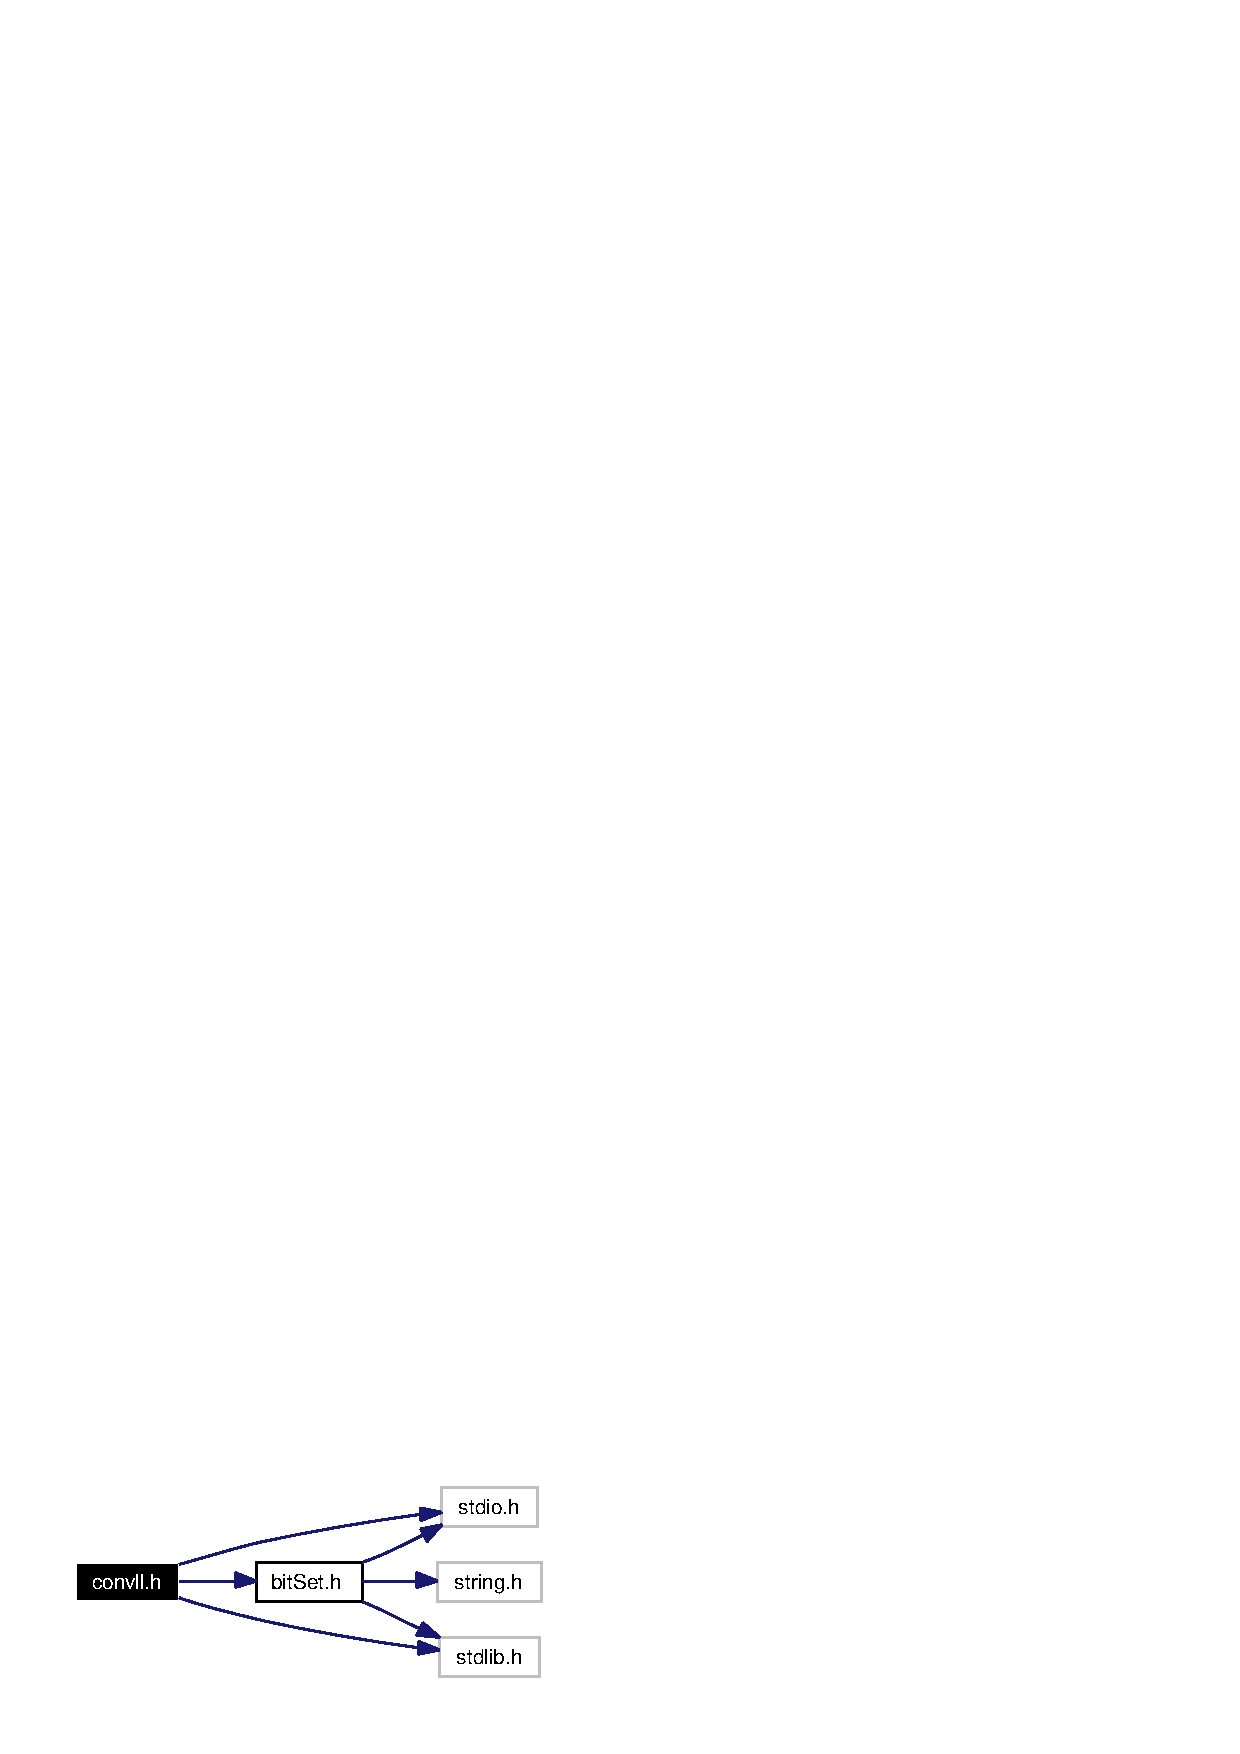
\includegraphics[width=130pt]{convll_8h__incl}
\end{center}
\end{figure}


This graph shows which files directly or indirectly include this file:\begin{figure}[H]
\begin{center}
\leavevmode
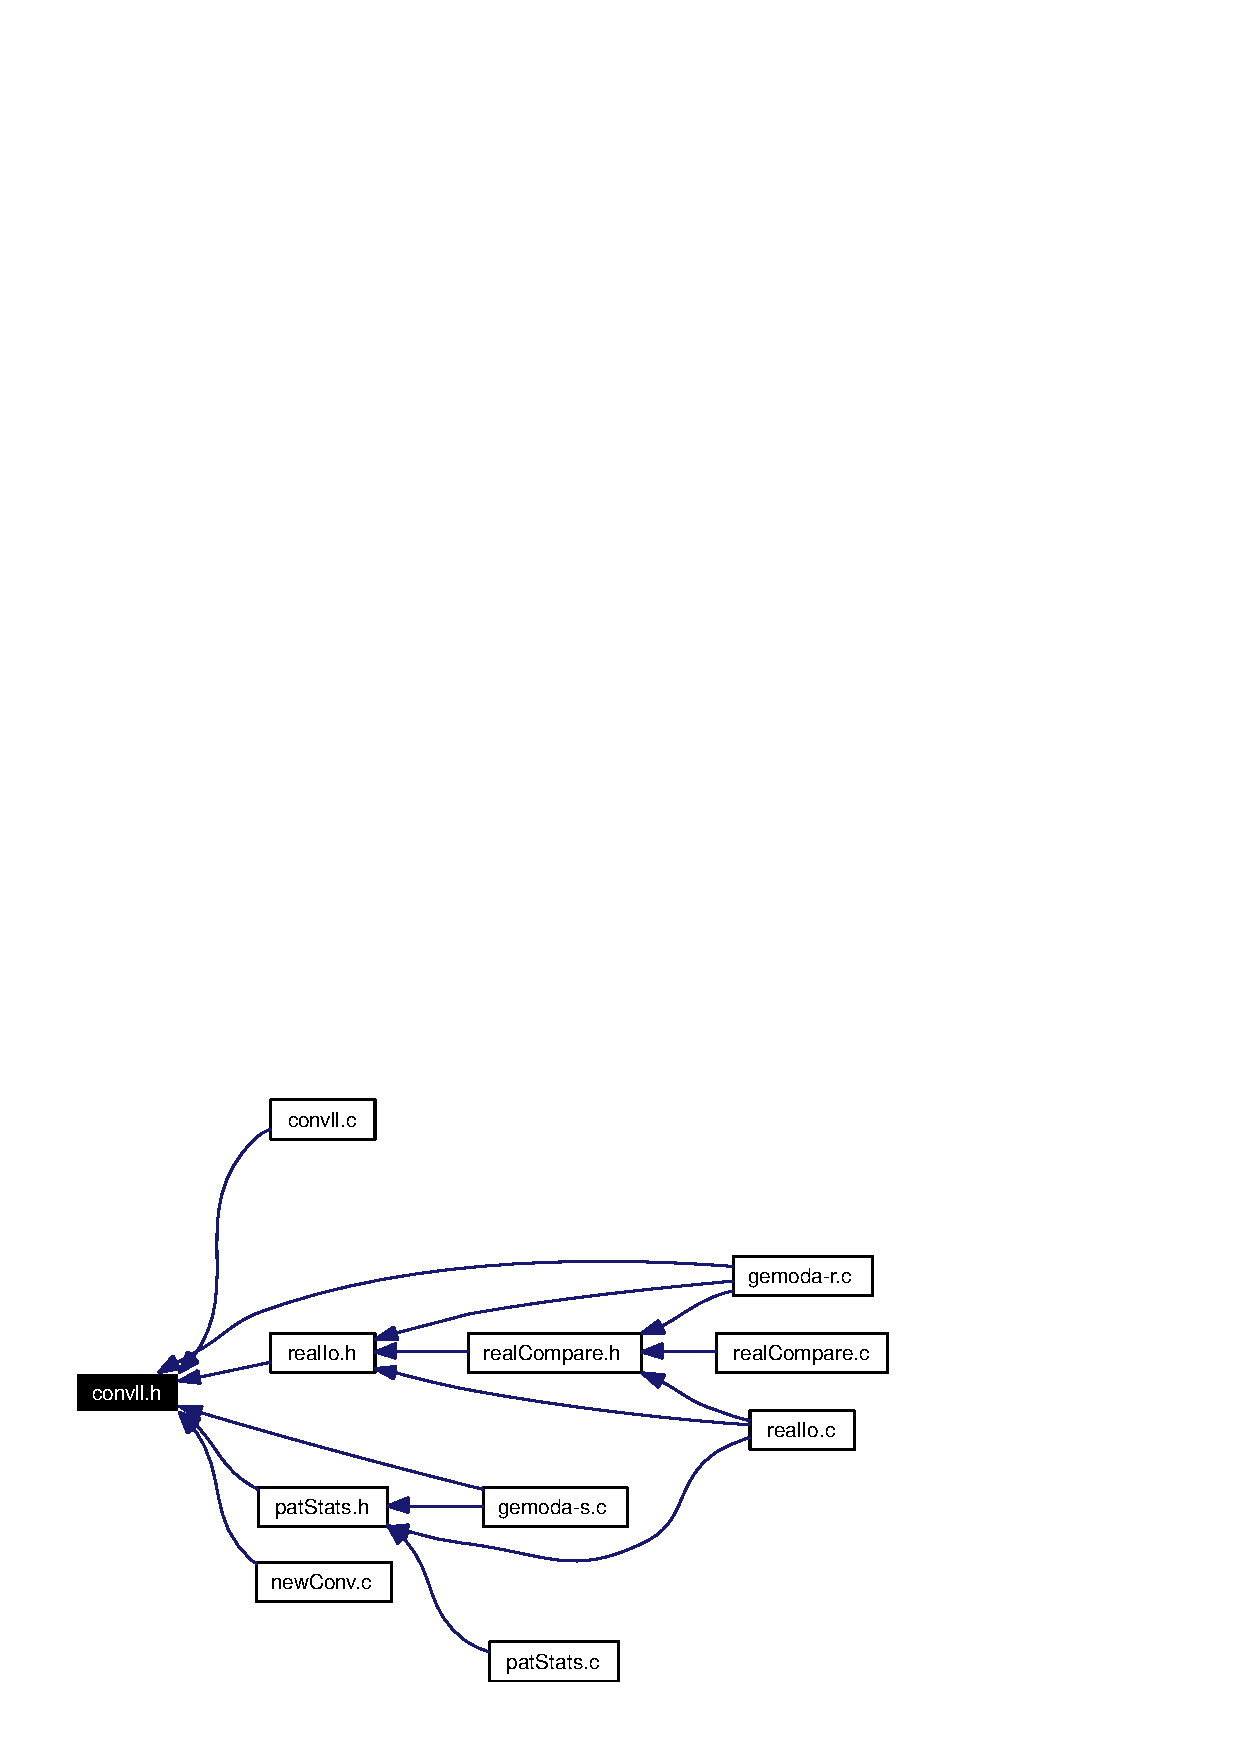
\includegraphics[width=213pt]{convll_8h__dep__incl}
\end{center}
\end{figure}
\subsection*{Data Structures}
\begin{CompactItemize}
\item 
struct \hyperlink{structcSet__t}{c\-Set\_\-t}
\item 
struct \hyperlink{structcnode}{cnode}
\item 
struct \hyperlink{structmnode}{mnode}
\end{CompactItemize}
\subsection*{Typedefs}
\begin{CompactItemize}
\item 
typedef \hyperlink{structcnode}{cnode} \hyperlink{convll_8h_a0}{cll\_\-t}
\item 
typedef \hyperlink{structmnode}{mnode} \hyperlink{convll_8h_a1}{mll\_\-t}
\end{CompactItemize}
\subsection*{Functions}
\begin{CompactItemize}
\item 
\hyperlink{structcnode}{cll\_\-t} $\ast$ \hyperlink{convll_8h_a2}{push\-Cll} (\hyperlink{structcnode}{cll\_\-t} $\ast$head)
\item 
\hyperlink{structcnode}{cll\_\-t} $\ast$ \hyperlink{convll_8h_a3}{pop\-Cll} (\hyperlink{structcnode}{cll\_\-t} $\ast$head)
\item 
\hyperlink{structcnode}{cll\_\-t} $\ast$ \hyperlink{convll_8h_a4}{pop\-All\-Cll} (\hyperlink{structcnode}{cll\_\-t} $\ast$head)
\item 
int \hyperlink{convll_8h_a5}{print\-Cll} (\hyperlink{structcnode}{cll\_\-t} $\ast$head)
\item 
\hyperlink{structcnode}{cll\_\-t} $\ast$ \hyperlink{convll_8h_a6}{inithead\-Cll} (\hyperlink{structcnode}{cll\_\-t} $\ast$head, \hyperlink{structcSet__t}{c\-Set\_\-t} $\ast$newset)
\item 
\hyperlink{structcnode}{cll\_\-t} $\ast$ \hyperlink{convll_8h_a7}{pushc\-Set} (\hyperlink{structcnode}{cll\_\-t} $\ast$head, \hyperlink{structcSet__t}{c\-Set\_\-t} $\ast$newset)
\item 
\hyperlink{structcnode}{cll\_\-t} $\ast$ \hyperlink{convll_8h_a8}{push\-Clique} (\hyperlink{structbitSet__t}{bit\-Set\_\-t} $\ast$clique, \hyperlink{structcnode}{cll\_\-t} $\ast$head, int $\ast$index\-To\-Seq, int p)
\item 
\hyperlink{structmnode}{mll\_\-t} $\ast$ \hyperlink{convll_8h_a9}{push\-Mem\-Stack} (\hyperlink{structmnode}{mll\_\-t} $\ast$head, int clique\-Num)
\item 
\hyperlink{structmnode}{mll\_\-t} $\ast$ \hyperlink{convll_8h_a10}{pop\-Mem\-Stack} (\hyperlink{structmnode}{mll\_\-t} $\ast$head)
\item 
\hyperlink{structmnode}{mll\_\-t} $\ast$ \hyperlink{convll_8h_a11}{pop\-Whole\-Mem\-Stack} (\hyperlink{structmnode}{mll\_\-t} $\ast$head)
\item 
\hyperlink{structmnode}{mll\_\-t} $\ast$$\ast$ \hyperlink{convll_8h_a12}{add\-To\-Stacks} (\hyperlink{structcnode}{cll\_\-t} $\ast$node, \hyperlink{structmnode}{mll\_\-t} $\ast$$\ast$member\-Stacks)
\item 
\hyperlink{structmnode}{mll\_\-t} $\ast$$\ast$ \hyperlink{convll_8h_a13}{fill\-Member\-Stacks} (\hyperlink{structcnode}{cll\_\-t} $\ast$head, \hyperlink{structmnode}{mll\_\-t} $\ast$$\ast$member\-Stacks)
\item 
\hyperlink{structmnode}{mll\_\-t} $\ast$$\ast$ \hyperlink{convll_8h_a14}{empty\-Member\-Stacks} (\hyperlink{structmnode}{mll\_\-t} $\ast$$\ast$member\-Stacks, int size)
\item 
void \hyperlink{convll_8h_a15}{print\-Member\-Stacks} (\hyperlink{structmnode}{mll\_\-t} $\ast$$\ast$member\-Stacks, int size)
\item 
\hyperlink{structbitSet__t}{bit\-Set\_\-t} $\ast$ \hyperlink{convll_8h_a16}{search\-Mems\-With\-List} (int $\ast$list, int listsize, \hyperlink{structmnode}{mll\_\-t} $\ast$$\ast$mem\-List, int num\-Offsets, \hyperlink{structbitSet__t}{bit\-Set\_\-t} $\ast$queue)
\item 
\hyperlink{structbitSet__t}{bit\-Set\_\-t} $\ast$ \hyperlink{convll_8h_a17}{set\-Stack\-True} (\hyperlink{structmnode}{mll\_\-t} $\ast$$\ast$mem\-List, int i, \hyperlink{structbitSet__t}{bit\-Set\_\-t} $\ast$queue)
\item 
\hyperlink{structcnode}{cll\_\-t} $\ast$ \hyperlink{convll_8h_a18}{single\-Clique\-Conv} (\hyperlink{structcnode}{cll\_\-t} $\ast$head, int first\-Clique, \hyperlink{structcnode}{cll\_\-t} $\ast$$\ast$first\-Guess, int second\-Clique, \hyperlink{structcnode}{cll\_\-t} $\ast$$\ast$second\-Guess, \hyperlink{structcnode}{cll\_\-t} $\ast$next\-Phase, \hyperlink{structbitSet__t}{bit\-Set\_\-t} $\ast$print\-Status, int support)
\item 
\hyperlink{structmnode}{mll\_\-t} $\ast$ \hyperlink{convll_8h_a19}{merge\-Intersect} (\hyperlink{structcnode}{cll\_\-t} $\ast$first, \hyperlink{structcnode}{cll\_\-t} $\ast$second, \hyperlink{structmnode}{mll\_\-t} $\ast$intersection, \hyperlink{structbitSet__t}{bit\-Set\_\-t} $\ast$print\-Status, int $\ast$new\-Support)
\item 
\hyperlink{structcnode}{cll\_\-t} $\ast$ \hyperlink{convll_8h_a20}{push\-Conv\-Clique} (\hyperlink{structmnode}{mll\_\-t} $\ast$clique, \hyperlink{structcnode}{cll\_\-t} $\ast$head)
\item 
\hyperlink{structcSet__t}{c\-Set\_\-t} $\ast$ \hyperlink{convll_8h_a21}{mll\-To\-CSet} (\hyperlink{structmnode}{mll\_\-t} $\ast$clique)
\item 
\hyperlink{structcSet__t}{c\-Set\_\-t} $\ast$ \hyperlink{convll_8h_a22}{bit\-Set\-To\-CSet} (\hyperlink{structbitSet__t}{bit\-Set\_\-t} $\ast$clique)
\item 
\hyperlink{structcnode}{cll\_\-t} $\ast$ \hyperlink{convll_8h_a23}{whole\-Clique\-Conv} (\hyperlink{structcnode}{cll\_\-t} $\ast$head, \hyperlink{structcnode}{cll\_\-t} $\ast$node, \hyperlink{structcnode}{cll\_\-t} $\ast$$\ast$first\-Guess, \hyperlink{structmnode}{mll\_\-t} $\ast$$\ast$mem\-List, int num\-Offsets, \hyperlink{structcnode}{cll\_\-t} $\ast$next\-Phase, \hyperlink{structbitSet__t}{bit\-Set\_\-t} $\ast$print\-Status, int support)
\item 
\hyperlink{structcnode}{cll\_\-t} $\ast$ \hyperlink{convll_8h_a24}{whole\-Round\-Conv} (\hyperlink{structcnode}{cll\_\-t} $\ast$$\ast$head, \hyperlink{structmnode}{mll\_\-t} $\ast$$\ast$mem\-List, int num\-Offsets, int support, int length, \hyperlink{structcnode}{cll\_\-t} $\ast$$\ast$all\-Cliques)
\item 
\hyperlink{structcnode}{cll\_\-t} $\ast$ \hyperlink{convll_8h_a25}{complete\-Conv} (\hyperlink{structcnode}{cll\_\-t} $\ast$$\ast$head, int support, int num\-Offsets, int min\-Length, int $\ast$index\-To\-Seq, int p)
\item 
int \hyperlink{convll_8h_a26}{print\-Cll\-Pattern} (\hyperlink{structcnode}{cll\_\-t} $\ast$node, int length)
\item 
int \hyperlink{convll_8h_a27}{uniq\-Clique} (\hyperlink{structcSet__t}{c\-Set\_\-t} $\ast$clique, \hyperlink{structcnode}{cll\_\-t} $\ast$head)
\item 
\hyperlink{structcnode}{cll\_\-t} $\ast$ \hyperlink{convll_8h_a28}{swap\-Nodec\-Set} (\hyperlink{structcnode}{cll\_\-t} $\ast$head, int node, \hyperlink{structcSet__t}{c\-Set\_\-t} $\ast$new\-Clique)
\item 
int \hyperlink{convll_8h_a29}{yank\-Cll} (\hyperlink{structcnode}{cll\_\-t} $\ast$$\ast$head, \hyperlink{structcnode}{cll\_\-t} $\ast$prev, \hyperlink{structcnode}{cll\_\-t} $\ast$$\ast$curr, \hyperlink{structcnode}{cll\_\-t} $\ast$$\ast$all\-Cliques, int length)
\item 
\hyperlink{structcnode}{cll\_\-t} $\ast$ \hyperlink{convll_8h_a30}{remove\-Supers} (\hyperlink{structcnode}{cll\_\-t} $\ast$head, int node, \hyperlink{structcSet__t}{c\-Set\_\-t} $\ast$new\-Clique)
\end{CompactItemize}


\subsection*{Detailed Description}
This header file contains declarations and definitions for dealing with different kinds of sets that are used throughout the convolution stage of Gemoda.

Definition in file \hyperlink{convll_8h-source}{convll.h}.

\subsection*{Typedef Documentation}
\hypertarget{convll_8h_a0}{
\index{convll.h@{convll.h}!cll_t@{cll\_\-t}}
\index{cll_t@{cll\_\-t}!convll.h@{convll.h}}
\subsubsection[cll\_\-t]{\setlength{\rightskip}{0pt plus 5cm}typedef struct \hyperlink{structcnode}{cnode}  \hyperlink{structcnode}{cll\_\-t}}}
\label{convll_8h_a0}


This data structure is a linked list for storing cliques. Each member of the linked list has a set, an ID number, a length (which gives the number of characters in the motif), a pointer to the next member of the linked list, and a floating-point number for storing statistical information.\hypertarget{convll_8h_a1}{
\index{convll.h@{convll.h}!mll_t@{mll\_\-t}}
\index{mll_t@{mll\_\-t}!convll.h@{convll.h}}
\subsubsection[mll\_\-t]{\setlength{\rightskip}{0pt plus 5cm}typedef struct \hyperlink{structmnode}{mnode}  \hyperlink{structmnode}{mll\_\-t}}}
\label{convll_8h_a1}


This data structure is just a link to list of integers used for bookkeeping during the convolution stage.

\subsection*{Function Documentation}
\hypertarget{convll_8h_a12}{
\index{convll.h@{convll.h}!addToStacks@{addToStacks}}
\index{addToStacks@{addToStacks}!convll.h@{convll.h}}
\subsubsection[addToStacks]{\setlength{\rightskip}{0pt plus 5cm}\hyperlink{structmnode}{mll\_\-t}$\ast$$\ast$ add\-To\-Stacks (\hyperlink{structcnode}{cll\_\-t} $\ast$ {\em node}, \hyperlink{structmnode}{mll\_\-t} $\ast$$\ast$ {\em member\-Stacks})}}
\label{convll_8h_a12}


For one clique, it adds membership for that clique to all of its members' member stacks. Input: a specific clique in a clique linked list, an array of member stacks. Output: the array of updated member stacks.

Definition at line 425 of file convll.c.

References cnode::id, c\-Set\_\-t::members, push\-Mem\-Stack(), and cnode::set.

Referenced by fill\-Member\-Stacks().



\hypertarget{convll_8h_a22}{
\index{convll.h@{convll.h}!bitSetToCSet@{bitSetToCSet}}
\index{bitSetToCSet@{bitSetToCSet}!convll.h@{convll.h}}
\subsubsection[bitSetToCSet]{\setlength{\rightskip}{0pt plus 5cm}\hyperlink{structcSet__t}{c\-Set\_\-t}$\ast$ bit\-Set\-To\-CSet (\hyperlink{structbitSet__t}{bit\-Set\_\-t} $\ast$ {\em clique})}}
\label{convll_8h_a22}


Converts a \hyperlink{structbitSet__t}{bit\-Set\_\-t} to a \hyperlink{structcSet__t}{c\-Set\_\-t} for the purposes of pushing it onto a linked list of cliques. The \hyperlink{structbitSet__t}{bit\-Set\_\-t} data structure is used for massive comparisons during clique-finding but is unwieldy/inefficient when it is known that the structure is sparse. The \hyperlink{structcSet__t}{c\-Set\_\-t} allows for efficient comparison of sparse bit\-Set\_\-t's. Use this just before pushing a newly-discovered clique onto a clique linked list. Input: a new clique in the form of a \hyperlink{structbitSet__t}{bit\-Set\_\-t}. Output: the same clique in the form of a \hyperlink{structcSet__t}{c\-Set\_\-t}.

Definition at line 193 of file convll.c.

References count\-Set(), c\-Set\_\-t::members, next\-Bit\-Bit\-Set(), and c\-Set\_\-t::size.

Referenced by push\-Clique(), and whole\-Clique\-Conv().



\hypertarget{convll_8h_a25}{
\index{convll.h@{convll.h}!completeConv@{completeConv}}
\index{completeConv@{completeConv}!convll.h@{convll.h}}
\subsubsection[completeConv]{\setlength{\rightskip}{0pt plus 5cm}\hyperlink{structcnode}{cll\_\-t}$\ast$ complete\-Conv (\hyperlink{structcnode}{cll\_\-t} $\ast$$\ast$ {\em head}, int {\em support}, int {\em num\-Offsets}, int {\em min\-Length}, int $\ast$ {\em index\-To\-Seq}, int {\em p})}}
\label{convll_8h_a25}


Performs complete convolution given the starting list of cliques. Input: a pointer to the head of the initial clique linked list, the minimum support criterion value, the number of offsets in the sequence set, the minimum length of motifs (which is the length of motifs in the initial clique linked list), the index/Sequence data structure, and the value of the -p flag to prune based on unique sequence occurrences. Output: a linked list of all maximal cliques based on the initial clique linked list.

Definition at line 1267 of file convll.c.

References empty\-Member\-Stacks(), fill\-Member\-Stacks(), pop\-All\-Cll(), prune\-Cll(), and whole\-Round\-Conv().

Referenced by convolve().



\hypertarget{convll_8h_a14}{
\index{convll.h@{convll.h}!emptyMemberStacks@{emptyMemberStacks}}
\index{emptyMemberStacks@{emptyMemberStacks}!convll.h@{convll.h}}
\subsubsection[emptyMemberStacks]{\setlength{\rightskip}{0pt plus 5cm}\hyperlink{structmnode}{mll\_\-t}$\ast$$\ast$ empty\-Member\-Stacks (\hyperlink{structmnode}{mll\_\-t} $\ast$$\ast$ {\em member\-Stacks}, int {\em size})}}
\label{convll_8h_a14}


After we have performed a round of convolution, this \char`\"{}empties\char`\"{} the member stacks by popping all nodes off each member linked list. Input: array of member linked lists, the size of that array (total number of offsets). Output: the array of now-empty member linked lists.

Definition at line 474 of file convll.c.

References pop\-Whole\-Mem\-Stack().

Referenced by complete\-Conv().



\hypertarget{convll_8h_a13}{
\index{convll.h@{convll.h}!fillMemberStacks@{fillMemberStacks}}
\index{fillMemberStacks@{fillMemberStacks}!convll.h@{convll.h}}
\subsubsection[fillMemberStacks]{\setlength{\rightskip}{0pt plus 5cm}\hyperlink{structmnode}{mll\_\-t}$\ast$$\ast$ fill\-Member\-Stacks (\hyperlink{structcnode}{cll\_\-t} $\ast$ {\em head}, \hyperlink{structmnode}{mll\_\-t} $\ast$$\ast$ {\em member\-Stacks})}}
\label{convll_8h_a13}


Fills the entire member\-Stacks data structure by calling add\-To\-Stacks for each clique in the clique linked list. Input: head of a clique linked list, array of member linked lists. Output: the array of updated member linked lists.

Definition at line 455 of file convll.c.

References add\-To\-Stacks(), and cnode::next.

Referenced by complete\-Conv().



\hypertarget{convll_8h_a6}{
\index{convll.h@{convll.h}!initheadCll@{initheadCll}}
\index{initheadCll@{initheadCll}!convll.h@{convll.h}}
\subsubsection[initheadCll]{\setlength{\rightskip}{0pt plus 5cm}\hyperlink{structcnode}{cll\_\-t}$\ast$ inithead\-Cll (\hyperlink{structcnode}{cll\_\-t} $\ast$ {\em head}, \hyperlink{structcSet__t}{c\-Set\_\-t} $\ast$ {\em newset})}}
\label{convll_8h_a6}


Initializes the empty head of a linked list by adding a set to that head. Note: this is only called immediately after pushing onto a cll, because the push always creates a new empty head. This function should not be called by the user; see pushc\-Set. Input: head of a linked list, pointer to a \hyperlink{structcSet__t}{c\-Set\_\-t} list of clique members. Output: head of a linked list.

Definition at line 156 of file convll.c.

References cnode::set.

Referenced by pushc\-Set().



\hypertarget{convll_8h_a19}{
\index{convll.h@{convll.h}!mergeIntersect@{mergeIntersect}}
\index{mergeIntersect@{mergeIntersect}!convll.h@{convll.h}}
\subsubsection[mergeIntersect]{\setlength{\rightskip}{0pt plus 5cm}\hyperlink{structmnode}{mll\_\-t}$\ast$ merge\-Intersect (\hyperlink{structcnode}{cll\_\-t} $\ast$ {\em first}, \hyperlink{structcnode}{cll\_\-t} $\ast$ {\em second}, \hyperlink{structmnode}{mll\_\-t} $\ast$ {\em intersection}, \hyperlink{structbitSet__t}{bit\-Set\_\-t} $\ast$ {\em printstatus}, int $\ast$ {\em new\-Support})}}
\label{convll_8h_a19}


Convolves two cliques in a non-commutative manner. It finds which members of the first clique are immediately followed by a member in the second clique. Input: pointer to the location in the linked list of the first clique to be convolved, pointer to the location in the linked list of the second clique to be convolved, a member linked list used to store the intersection of the two cliques, the printstatus bit\-Set, and a pointer to an integer with the support of the clique formed by convolution. Output: a member linked list with the intersection of the two cliques, plus the side effect of that intersection's cardinality being stored in the integer pointed to by new\-Support.

Definition at line 671 of file convll.c.

References c\-Set\_\-t::members, push\-Mem\-Stack(), cnode::set, and c\-Set\_\-t::size.

Referenced by single\-Clique\-Conv().



\hypertarget{convll_8h_a21}{
\index{convll.h@{convll.h}!mllToCSet@{mllToCSet}}
\index{mllToCSet@{mllToCSet}!convll.h@{convll.h}}
\subsubsection[mllToCSet]{\setlength{\rightskip}{0pt plus 5cm}\hyperlink{structcSet__t}{c\-Set\_\-t}$\ast$ mll\-To\-CSet (\hyperlink{structmnode}{mll\_\-t} $\ast$ {\em clique})}}
\label{convll_8h_a21}


Turns a member linked list used to store the intersection of two cliques into something more useful: a \hyperlink{structcSet__t}{c\-Set\_\-t} structure. Input: a clique in mll\_\-t form. Output: a clique in \hyperlink{structcSet__t}{c\-Set\_\-t} form.

Definition at line 1022 of file convll.c.

References mnode::clique\-Membership, c\-Set\_\-t::members, mnode::next, and c\-Set\_\-t::size.

Referenced by push\-Conv\-Clique().



\hypertarget{convll_8h_a4}{
\index{convll.h@{convll.h}!popAllCll@{popAllCll}}
\index{popAllCll@{popAllCll}!convll.h@{convll.h}}
\subsubsection[popAllCll]{\setlength{\rightskip}{0pt plus 5cm}\hyperlink{structcnode}{cll\_\-t}$\ast$ pop\-All\-Cll (\hyperlink{structcnode}{cll\_\-t} $\ast$ {\em head})}}
\label{convll_8h_a4}


Shortcut function to pop all of the members of a linked list. Input: head of a linked list. Output: head of a now-empty linked list.

Definition at line 101 of file convll.c.

References pop\-Cll().

Referenced by complete\-Conv(), and main().



\hypertarget{convll_8h_a3}{
\index{convll.h@{convll.h}!popCll@{popCll}}
\index{popCll@{popCll}!convll.h@{convll.h}}
\subsubsection[popCll]{\setlength{\rightskip}{0pt plus 5cm}\hyperlink{structcnode}{cll\_\-t}$\ast$ pop\-Cll (\hyperlink{structcnode}{cll\_\-t} $\ast$ {\em head})}}
\label{convll_8h_a3}


Removes the head of the clique linked list, returns the new head of the clique linked list, and frees the memory occupied by the old head. Input: head of a linked list. Output: head of a linked list.

Definition at line 60 of file convll.c.

References c\-Set\_\-t::members, cnode::next, and cnode::set.

Referenced by pop\-All\-Cll().



\hypertarget{convll_8h_a10}{
\index{convll.h@{convll.h}!popMemStack@{popMemStack}}
\index{popMemStack@{popMemStack}!convll.h@{convll.h}}
\subsubsection[popMemStack]{\setlength{\rightskip}{0pt plus 5cm}\hyperlink{structmnode}{mll\_\-t}$\ast$ pop\-Mem\-Stack (\hyperlink{structmnode}{mll\_\-t} $\ast$ {\em head})}}
\label{convll_8h_a10}


Pops the head off of a single member linked list. Input: head of a member linked list. Output: the new head of a member linked list after popping one item.

Definition at line 388 of file convll.c.

References mnode::next.

Referenced by pop\-Whole\-Mem\-Stack().



\hypertarget{convll_8h_a11}{
\index{convll.h@{convll.h}!popWholeMemStack@{popWholeMemStack}}
\index{popWholeMemStack@{popWholeMemStack}!convll.h@{convll.h}}
\subsubsection[popWholeMemStack]{\setlength{\rightskip}{0pt plus 5cm}\hyperlink{structmnode}{mll\_\-t}$\ast$ pop\-Whole\-Mem\-Stack (\hyperlink{structmnode}{mll\_\-t} $\ast$ {\em head})}}
\label{convll_8h_a11}


Pops all items off of a member linked list. Input: head of a member linked list. Output: empty head of a member linked list.

Definition at line 410 of file convll.c.

References pop\-Mem\-Stack().

Referenced by empty\-Member\-Stacks(), and single\-Clique\-Conv().



\hypertarget{convll_8h_a5}{
\index{convll.h@{convll.h}!printCll@{printCll}}
\index{printCll@{printCll}!convll.h@{convll.h}}
\subsubsection[printCll]{\setlength{\rightskip}{0pt plus 5cm}int print\-Cll (\hyperlink{structcnode}{cll\_\-t} $\ast$ {\em head})}}
\label{convll_8h_a5}


Prints the members (cliques) of a linked list in the format: {\em id\/} = unique id number of clique within linked list; {\em Length\/} = number of members of clique, if available; {\em Size\/} = length of each member of clique; {\em Members\/} = newline-separated list of members of the clique. Input: head of a linked list. Output: Gives text output, returns (meaningless) exit value.

Definition at line 118 of file convll.c.

References cnode::id, cnode::length, c\-Set\_\-t::members, cnode::next, cnode::set, and c\-Set\_\-t::size.



\hypertarget{convll_8h_a26}{
\index{convll.h@{convll.h}!printCllPattern@{printCllPattern}}
\index{printCllPattern@{printCllPattern}!convll.h@{convll.h}}
\subsubsection[printCllPattern]{\setlength{\rightskip}{0pt plus 5cm}int print\-Cll\-Pattern (\hyperlink{structcnode}{cll\_\-t} $\ast$ {\em node}, int {\em length})}}
\label{convll_8h_a26}


Prints out the contents of a clique linked list node in this format: {\em support\/} = number of motif occurrences ({\em id\/} = some id number); {\em members\/} = newline-separated list of offsets. Input: a specific node to be output, the length of the motif inside it. Output: text per above, and an integer success value.

Definition at line 1328 of file convll.c.

References cnode::id, c\-Set\_\-t::members, cnode::set, and c\-Set\_\-t::size.



\hypertarget{convll_8h_a15}{
\index{convll.h@{convll.h}!printMemberStacks@{printMemberStacks}}
\index{printMemberStacks@{printMemberStacks}!convll.h@{convll.h}}
\subsubsection[printMemberStacks]{\setlength{\rightskip}{0pt plus 5cm}void print\-Member\-Stacks (\hyperlink{structmnode}{mll\_\-t} $\ast$$\ast$ {\em member\-Stacks}, int {\em size})}}
\label{convll_8h_a15}


Prints the contents of the member stacks. Input: array of member linked lists, size of that array (total number of offsets). Output: only text output/no return value.

Definition at line 491 of file convll.c.

References mnode::clique\-Membership, and mnode::next.



\hypertarget{convll_8h_a8}{
\index{convll.h@{convll.h}!pushClique@{pushClique}}
\index{pushClique@{pushClique}!convll.h@{convll.h}}
\subsubsection[pushClique]{\setlength{\rightskip}{0pt plus 5cm}\hyperlink{structcnode}{cll\_\-t}$\ast$ push\-Clique (\hyperlink{structbitSet__t}{bit\-Set\_\-t} $\ast$ {\em clique}, \hyperlink{structcnode}{cll\_\-t} $\ast$ {\em head}, int $\ast$ {\em index\-To\-Seq}, int {\em p})}}
\label{convll_8h_a8}


Pushes a bit\-Set onto a clique linked list, performing all necessary manipulations in order to do so. Input: new clique in the form of a \hyperlink{structbitSet__t}{bit\-Set\_\-t}, head of a linked list, pointer to the index/sequence number data structure, integer value of the -p flag. Output: head of an updated clique linked list.

Definition at line 314 of file convll.c.

References bit\-Set\-To\-CSet(), check\-Cliquec\-Set(), cliquecounter, c\-Set\_\-t::members, and pushc\-Set().

Referenced by find\-Cliques(), and single\-Linkage().



\hypertarget{convll_8h_a2}{
\index{convll.h@{convll.h}!pushCll@{pushCll}}
\index{pushCll@{pushCll}!convll.h@{convll.h}}
\subsubsection[pushCll]{\setlength{\rightskip}{0pt plus 5cm}\hyperlink{structcnode}{cll\_\-t}$\ast$ push\-Cll (\hyperlink{structcnode}{cll\_\-t} $\ast$ {\em head})}}
\label{convll_8h_a2}


Pushes a new, empty head onto a linked list of cliques. Note: this should always be followed by a call to inithead\-Cll, as the head pushed on here is empty and will be meaningless without any members. This function should NOT be used by the user; see pushc\-Set. Input: head of a linked list. Output: head of a linked list.

Definition at line 26 of file convll.c.

References cnode::id, cnode::length, cnode::next, cnode::set, and cnode::stat.

Referenced by pushc\-Set().



\hypertarget{convll_8h_a20}{
\index{convll.h@{convll.h}!pushConvClique@{pushConvClique}}
\index{pushConvClique@{pushConvClique}!convll.h@{convll.h}}
\subsubsection[pushConvClique]{\setlength{\rightskip}{0pt plus 5cm}\hyperlink{structcnode}{cll\_\-t}$\ast$ push\-Conv\-Clique (\hyperlink{structmnode}{mll\_\-t} $\ast$ {\em clique}, \hyperlink{structcnode}{cll\_\-t} $\ast$ {\em head})}}
\label{convll_8h_a20}


Pushes a freshly-convolved clique, currently in mll\_\-t form, onto the clique linked list for the next level. Also checks to make sure that the convolved clique is unique, and if it isn't, it takes appropriate action. Input: a convolved clique in mll\_\-t form, the head of a clique linked list for the next level. Output: (potentially new) head of the clique linked list for the next level.

Definition at line 980 of file convll.c.

References c\-Set\_\-t::members, mll\-To\-CSet(), pushc\-Set(), remove\-Supers(), swap\-Nodec\-Set(), and uniq\-Clique().

Referenced by single\-Clique\-Conv().



\hypertarget{convll_8h_a7}{
\index{convll.h@{convll.h}!pushcSet@{pushcSet}}
\index{pushcSet@{pushcSet}!convll.h@{convll.h}}
\subsubsection[pushcSet]{\setlength{\rightskip}{0pt plus 5cm}\hyperlink{structcnode}{cll\_\-t}$\ast$ pushc\-Set (\hyperlink{structcnode}{cll\_\-t} $\ast$ {\em head}, \hyperlink{structcSet__t}{c\-Set\_\-t} $\ast$ {\em newset})}}
\label{convll_8h_a7}


Function that pushes the contents of a c\-Set (set of members of a clique) onto a linked list of cliques. Input: head of a linked list, new clique in the form of a \hyperlink{structcSet__t}{c\-Set\_\-t}. Output: head of a linked list.

Definition at line 174 of file convll.c.

References inithead\-Cll(), and push\-Cll().

Referenced by push\-Clique(), and push\-Conv\-Clique().



\hypertarget{convll_8h_a9}{
\index{convll.h@{convll.h}!pushMemStack@{pushMemStack}}
\index{pushMemStack@{pushMemStack}!convll.h@{convll.h}}
\subsubsection[pushMemStack]{\setlength{\rightskip}{0pt plus 5cm}\hyperlink{structmnode}{mll\_\-t}$\ast$ push\-Mem\-Stack (\hyperlink{structmnode}{mll\_\-t} $\ast$ {\em head}, int {\em clique\-Num})}}
\label{convll_8h_a9}


This begins code for the member linked lists. A single one of these linked lists functions somewhat similarly to the clique linked lists, though with less information stored. Functionally, an array of member linked lists is used to access the \char`\"{}inverse\char`\"{} of what is contained in the clique linked lists. That is, we would like to be able to look up the cliques that a given node is a member of, so we have an array of member linked lists of size equal to the number of nodes.

This function pushes a single clique membership onto a node's member stack. Input: the head of a single member linked list, a clique number to be added. Output: the head of a single member linked list.

Definition at line 358 of file convll.c.

References mnode::clique\-Membership, and mnode::next.

Referenced by add\-To\-Stacks(), and merge\-Intersect().



\hypertarget{convll_8h_a30}{
\index{convll.h@{convll.h}!removeSupers@{removeSupers}}
\index{removeSupers@{removeSupers}!convll.h@{convll.h}}
\subsubsection[removeSupers]{\setlength{\rightskip}{0pt plus 5cm}\hyperlink{structcnode}{cll\_\-t}$\ast$ remove\-Supers (\hyperlink{structcnode}{cll\_\-t} $\ast$ {\em head}, int {\em node}, \hyperlink{structcSet__t}{c\-Set\_\-t} $\ast$ {\em new\-Clique})}}
\label{convll_8h_a30}


This function finds all cliques in a linked list of which the proposed clique is a superset. It starts looking AFTER the first clique which has already been found to be a subset. In some senses, it is just a continuation of the uniqclique function in order to take advantage of the fact that though a proposed clique can only be a subset of one existing next-level clique, it can be a superset of many existing next- level cliques. Input: head of a clique linked list, the id of the first node found to be a subset of the proposed clique, and the proposed clique (in \hyperlink{structcSet__t}{c\-Set\_\-t} form). Output: the head of the clique linked list with all but the first subset (which was passed as an argument) removed. This function is now ready for swap\-Node to be called.

Definition at line 849 of file convll.c.

References cnode::id, c\-Set\_\-t::members, cnode::next, cnode::set, and c\-Set\_\-t::size.

Referenced by push\-Conv\-Clique().



\hypertarget{convll_8h_a16}{
\index{convll.h@{convll.h}!searchMemsWithList@{searchMemsWithList}}
\index{searchMemsWithList@{searchMemsWithList}!convll.h@{convll.h}}
\subsubsection[searchMemsWithList]{\setlength{\rightskip}{0pt plus 5cm}\hyperlink{structbitSet__t}{bit\-Set\_\-t}$\ast$ search\-Mems\-With\-List (int $\ast$ {\em list}, int {\em listsize}, \hyperlink{structmnode}{mll\_\-t} $\ast$$\ast$ {\em mem\-List}, int {\em num\-Offsets}, \hyperlink{structbitSet__t}{bit\-Set\_\-t} $\ast$ {\em queue})}}
\label{convll_8h_a16}


Creates one large queue by calling \char`\"{}set\-Stack\-True\char`\"{} for each member of a list of offsets. This then creates the union of clique membership for all offsets in the list being searched. Input: an array of offset numbers, the length of that array, an array of member linked lists, the length of that array (the total number of offsets), and a \hyperlink{structbitSet__t}{bit\-Set\_\-t} to store the union/queue. Output: the union/queue in a \hyperlink{structbitSet__t}{bit\-Set\_\-t} structure.

Definition at line 540 of file convll.c.

References empty\-Set(), and set\-Stack\-True().

Referenced by whole\-Clique\-Conv().



\hypertarget{convll_8h_a17}{
\index{convll.h@{convll.h}!setStackTrue@{setStackTrue}}
\index{setStackTrue@{setStackTrue}!convll.h@{convll.h}}
\subsubsection[setStackTrue]{\setlength{\rightskip}{0pt plus 5cm}\hyperlink{structbitSet__t}{bit\-Set\_\-t}$\ast$ set\-Stack\-True (\hyperlink{structmnode}{mll\_\-t} $\ast$$\ast$ {\em mem\-List}, int {\em i}, \hyperlink{structbitSet__t}{bit\-Set\_\-t} $\ast$ {\em queue})}}
\label{convll_8h_a17}


Adds all of the members of a given stack to a \char`\"{}queue\char`\"{} in the form of a \hyperlink{structbitSet__t}{bit\-Set\_\-t} data structure. That is, for each clique in the member linked list, it sets the corresponding bit in the \hyperlink{structbitSet__t}{bit\-Set\_\-t} true. Input: array of member linked lists, an integer indicating a specific member linked list, and a \hyperlink{structbitSet__t}{bit\-Set\_\-t} of length $>$= the number of cliques in the current clique linked list. Ouput: the updated \hyperlink{structbitSet__t}{bit\-Set\_\-t} object.

Definition at line 516 of file convll.c.

References mnode::clique\-Membership, mnode::next, and set\-True().

Referenced by search\-Mems\-With\-List().



\hypertarget{convll_8h_a18}{
\index{convll.h@{convll.h}!singleCliqueConv@{singleCliqueConv}}
\index{singleCliqueConv@{singleCliqueConv}!convll.h@{convll.h}}
\subsubsection[singleCliqueConv]{\setlength{\rightskip}{0pt plus 5cm}\hyperlink{structcnode}{cll\_\-t}$\ast$ single\-Clique\-Conv (\hyperlink{structcnode}{cll\_\-t} $\ast$ {\em head}, int {\em first\-Clique}, \hyperlink{structcnode}{cll\_\-t} $\ast$$\ast$ {\em first\-Guess}, int {\em second\-Clique}, \hyperlink{structcnode}{cll\_\-t} $\ast$$\ast$ {\em second\-Guess}, \hyperlink{structcnode}{cll\_\-t} $\ast$ {\em next\-Phase}, \hyperlink{structbitSet__t}{bit\-Set\_\-t} $\ast$ {\em print\-Status}, int {\em support})}}
\label{convll_8h_a18}


Convolves one single clique against one other single clique. Note that this is non-commutative, so exchanging first\-Clique and second\-Clique will not give the same results. The \char`\"{}guess\char`\"{} pointers keep the location of the previous clique in the linked list so that we don't have to search the linked list from the beginning/end every time. We exploit our earlier tidiness in that we can reasonably guess that we will monotonically traverse down cliques. Input: head of the current clique linked list, the id number of the first clique, a pointer to a guess at the first clique, the id number of the second clique, a pointer to a guess at the second clique, the head of the clique linked list for the next round of convolution, a bit\-Set indicating which cliques should be output as maximal, and the minimum support flag. Output: the head of clique linked list for the next round of convolution (which may have changed if the two cliques could be convolved).

Definition at line 580 of file convll.c.

References cnode::id, merge\-Intersect(), cnode::next, pop\-Whole\-Mem\-Stack(), push\-Conv\-Clique(), cnode::set, set\-False(), and c\-Set\_\-t::size.

Referenced by whole\-Clique\-Conv().



\hypertarget{convll_8h_a28}{
\index{convll.h@{convll.h}!swapNodecSet@{swapNodecSet}}
\index{swapNodecSet@{swapNodecSet}!convll.h@{convll.h}}
\subsubsection[swapNodecSet]{\setlength{\rightskip}{0pt plus 5cm}\hyperlink{structcnode}{cll\_\-t}$\ast$ swap\-Nodec\-Set (\hyperlink{structcnode}{cll\_\-t} $\ast$ {\em head}, int {\em node}, \hyperlink{structcSet__t}{c\-Set\_\-t} $\ast$ {\em new\-Clique})}}
\label{convll_8h_a28}


Swaps out a node in a linked list that has been found to be a subset of a node that is not yet in the list. Input: the head of a clique linked list, a specific node within that linked list that is to be removed, and the new clique that is the superset of the node to be removed (in \hyperlink{structcSet__t}{c\-Set\_\-t} form). Output: the head of the altered clique linked list.

Definition at line 804 of file convll.c.

References cnode::id, c\-Set\_\-t::members, cnode::next, and cnode::set.

Referenced by push\-Conv\-Clique().



\hypertarget{convll_8h_a27}{
\index{convll.h@{convll.h}!uniqClique@{uniqClique}}
\index{uniqClique@{uniqClique}!convll.h@{convll.h}}
\subsubsection[uniqClique]{\setlength{\rightskip}{0pt plus 5cm}int uniq\-Clique (\hyperlink{structcSet__t}{c\-Set\_\-t} $\ast$ {\em cliquec\-Set}, \hyperlink{structcnode}{cll\_\-t} $\ast$ {\em head})}}
\label{convll_8h_a27}


Before we push a convolved clique onto the stack for the next level, this function ensures that it is not subsumed by and does not subsume any other clique currently on that stack. Input: a candidate clique for the next level in \hyperlink{structcSet__t}{c\-Set\_\-t} form, and the head of the clique linked list for the next level. Output: an integer indicating the status of the proposed clique with respect to the next level: -1 if the clique is unique, -2 if the clique is a subset/duplicate of an existing clique, or a clique id in the range \mbox{[}0,numcliques) representing the first clique of which the proposed one is a superset. Note that by executing this each time a clique is added to the next level, we ensure that if the new clique is not unique, it can only be a superset or a subset of some other clique; it cannot be both a strictly superset of one and a strictly subset of another. One of those other two cliques would have been identified in previous steps as being super- or sub-sets, so it is impossible for one clique now to be both a super and a subset.

Definition at line 729 of file convll.c.

References cnode::id, c\-Set\_\-t::members, cnode::next, cnode::set, and c\-Set\_\-t::size.

Referenced by push\-Conv\-Clique().



\hypertarget{convll_8h_a23}{
\index{convll.h@{convll.h}!wholeCliqueConv@{wholeCliqueConv}}
\index{wholeCliqueConv@{wholeCliqueConv}!convll.h@{convll.h}}
\subsubsection[wholeCliqueConv]{\setlength{\rightskip}{0pt plus 5cm}\hyperlink{structcnode}{cll\_\-t}$\ast$ whole\-Clique\-Conv (\hyperlink{structcnode}{cll\_\-t} $\ast$ {\em head}, \hyperlink{structcnode}{cll\_\-t} $\ast$ {\em node}, \hyperlink{structcnode}{cll\_\-t} $\ast$$\ast$ {\em first\-Guess}, \hyperlink{structmnode}{mll\_\-t} $\ast$$\ast$ {\em mem\-List}, int {\em num\-Offsets}, \hyperlink{structcnode}{cll\_\-t} $\ast$ {\em next\-Phase}, \hyperlink{structbitSet__t}{bit\-Set\_\-t} $\ast$ {\em print\-Status}, int {\em support})}}
\label{convll_8h_a23}


Convolves one single clique against all possible cliques that could possibly be convolved. It does not attempt to convolve all other cliques, but prunes that set by first looking at the offsets that are in the clique, then collecting all of the cliques who have members that are one greater than the offsets in this clique, and then convolving those cliques in a sort of \char`\"{}queue\char`\"{} using the \hyperlink{structbitSet__t}{bit\-Set\_\-t} data structure. Input: the head of the clique linked list for the current level, the current node being convolved against in the linked list, the location of the previous node in the form of a pointer to a \char`\"{}guess\char`\"{}, an array of member linked lists, the length of that array, the head of the clique linked list for the next level, a \hyperlink{structbitSet__t}{bit\-Set\_\-t} for the print\-Status of maximality, and the support criterion. Output: the head of the (possibly modified) clique linked list for the next level.

Definition at line 1081 of file convll.c.

References bit\-Set\-To\-CSet(), count\-Set(), delete\-Bit\-Set(), cnode::id, c\-Set\_\-t::members, new\-Bit\-Set(), search\-Mems\-With\-List(), cnode::set, single\-Clique\-Conv(), and c\-Set\_\-t::size.

Referenced by whole\-Round\-Conv().



\hypertarget{convll_8h_a24}{
\index{convll.h@{convll.h}!wholeRoundConv@{wholeRoundConv}}
\index{wholeRoundConv@{wholeRoundConv}!convll.h@{convll.h}}
\subsubsection[wholeRoundConv]{\setlength{\rightskip}{0pt plus 5cm}\hyperlink{structcnode}{cll\_\-t}$\ast$ whole\-Round\-Conv (\hyperlink{structcnode}{cll\_\-t} $\ast$$\ast$ {\em head}, \hyperlink{structmnode}{mll\_\-t} $\ast$$\ast$ {\em mem\-List}, int {\em num\-Offsets}, int {\em support}, int {\em length}, \hyperlink{structcnode}{cll\_\-t} $\ast$$\ast$ {\em all\-Cliques})}}
\label{convll_8h_a24}


Performs convolution on all cliques in a linked list by repeatedly calling whole\-Clique\-Conv. Input: pointer to the head of a clique linked list for the current level, array of member linked lists, length of that array, minimum support threshold, the current length of motifs, and a pointer to a linked list containing all cliques that will be printed out. Output: the head of the clique linked list for the next level of convolution.

Definition at line 1148 of file convll.c.

References check\-Bit(), delete\-Bit\-Set(), fill\-Set(), cnode::id, new\-Bit\-Set(), cnode::next, whole\-Clique\-Conv(), and yank\-Cll().

Referenced by complete\-Conv().



\hypertarget{convll_8h_a29}{
\index{convll.h@{convll.h}!yankCll@{yankCll}}
\index{yankCll@{yankCll}!convll.h@{convll.h}}
\subsubsection[yankCll]{\setlength{\rightskip}{0pt plus 5cm}int yank\-Cll (\hyperlink{structcnode}{cll\_\-t} $\ast$$\ast$ {\em head}, \hyperlink{structcnode}{cll\_\-t} $\ast$ {\em prev}, \hyperlink{structcnode}{cll\_\-t} $\ast$$\ast$ {\em curr}, \hyperlink{structcnode}{cll\_\-t} $\ast$$\ast$ {\em all\-Cliques}, int {\em length})}}
\label{convll_8h_a29}


Removes a clique from within a linked list in order to save it for later printing. This is done so that the cliques are not printed as they are convolved, but rather after all rounds of convolution are complete. Input: a pointer to the head of the current linked list, the clique prior to the one that is to be yanked (NULL if the clique to be yanked is the head), the clique that is to be yanked, a pointer to the head of the list with all cliques that are to be printed, and the length of the current motif. Output: Nothing is returned beyond a success integer, but it alters the current level cll\_\-t, the value of curr, and the linked list of all cliques that are to be printed.

Definition at line 1221 of file convll.c.

References cnode::id, and cnode::next.

Referenced by convolve(), and whole\-Round\-Conv().




\hypertarget{fastaSeqIO_8c}{
\section{Fasta\-Seq\-IO/fasta\-Seq\-IO.c File Reference}
\label{fastaSeqIO_8c}\index{FastaSeqIO/fastaSeqIO.c@{FastaSeqIO/fastaSeqIO.c}}
}
{\tt \#include \char`\"{}fasta\-Seq\-IO.h\char`\"{}}\par
{\tt \#include $<$stdlib.h$>$}\par
{\tt \#include $<$string.h$>$}\par
{\tt \#include $<$errno.h$>$}\par


Include dependency graph for fasta\-Seq\-IO.c:\begin{figure}[H]
\begin{center}
\leavevmode
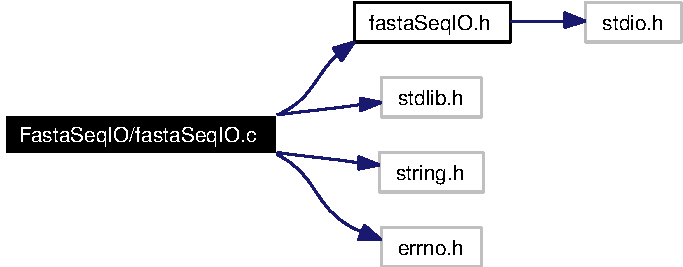
\includegraphics[width=181pt]{fastaSeqIO_8c__incl}
\end{center}
\end{figure}
\subsection*{Data Structures}
\begin{CompactItemize}
\item 
struct \hyperlink{structsSize__t}{s\-Size\_\-t}
\end{CompactItemize}
\subsection*{Defines}
\begin{CompactItemize}
\item 
\#define \hyperlink{fastaSeqIO_8c_a0}{BUFFER}~100000
\item 
\#define \hyperlink{fastaSeqIO_8c_a1}{BIG\_\-BUFFER}~1000000
\end{CompactItemize}
\subsection*{Functions}
\begin{CompactItemize}
\item 
int \hyperlink{fastaSeqIO_8c_a2}{print\-FSeq\-Sub\-Seq} (\hyperlink{structfSeq__t}{f\-Seq\_\-t} $\ast$seq, int start, int stop)
\item 
long \hyperlink{fastaSeqIO_8c_a3}{measure\-Line} (FILE $\ast$INPUT)
\item 
long \hyperlink{fastaSeqIO_8c_a4}{Count\-FSeqs} (FILE $\ast$INPUT)
\item 
long \hyperlink{fastaSeqIO_8c_a5}{count\-Lines} (FILE $\ast$INPUT)
\item 
int \hyperlink{fastaSeqIO_8c_a6}{init\-Aof\-FSeqs} (\hyperlink{structfSeq__t}{f\-Seq\_\-t} $\ast$aos, int num\-Seq)
\item 
char $\ast$$\ast$ \hyperlink{fastaSeqIO_8c_a7}{Read\-File} (FILE $\ast$INPUT, int $\ast$n)
\item 
\hyperlink{structfSeq__t}{f\-Seq\_\-t} $\ast$ \hyperlink{fastaSeqIO_8c_a8}{Read\-Txt\-Seqs} (FILE $\ast$INPUT, int $\ast$number\-Of\-Sequences)
\item 
\hyperlink{structfSeq__t}{f\-Seq\_\-t} $\ast$ \hyperlink{fastaSeqIO_8c_a9}{Read\-FSeqs} (FILE $\ast$INPUT, int $\ast$number\-Of\-Sequences)
\item 
int \hyperlink{fastaSeqIO_8c_a10}{Free\-FSeqs} (\hyperlink{structfSeq__t}{f\-Seq\_\-t} $\ast$array\-Of\-Sequences, int number\-Of\-Sequences)
\item 
int \hyperlink{fastaSeqIO_8c_a11}{Write\-FSeq\-A} (FILE $\ast$MY\_\-FILE, \hyperlink{structfSeq__t}{f\-Seq\_\-t} $\ast$array\-Of\-Sequences, int start, int stop)
\end{CompactItemize}


\subsection*{Define Documentation}
\hypertarget{fastaSeqIO_8c_a1}{
\index{fastaSeqIO.c@{fasta\-Seq\-IO.c}!BIG_BUFFER@{BIG\_\-BUFFER}}
\index{BIG_BUFFER@{BIG\_\-BUFFER}!fastaSeqIO.c@{fasta\-Seq\-IO.c}}
\subsubsection[BIG\_\-BUFFER]{\setlength{\rightskip}{0pt plus 5cm}\#define BIG\_\-BUFFER~1000000}}
\label{fastaSeqIO_8c_a1}




Definition at line 11 of file fasta\-Seq\-IO.c.\hypertarget{fastaSeqIO_8c_a0}{
\index{fastaSeqIO.c@{fasta\-Seq\-IO.c}!BUFFER@{BUFFER}}
\index{BUFFER@{BUFFER}!fastaSeqIO.c@{fasta\-Seq\-IO.c}}
\subsubsection[BUFFER]{\setlength{\rightskip}{0pt plus 5cm}\#define BUFFER~100000}}
\label{fastaSeqIO_8c_a0}




Definition at line 10 of file fasta\-Seq\-IO.c.

\subsection*{Function Documentation}
\hypertarget{fastaSeqIO_8c_a4}{
\index{fastaSeqIO.c@{fasta\-Seq\-IO.c}!CountFSeqs@{CountFSeqs}}
\index{CountFSeqs@{CountFSeqs}!fastaSeqIO.c@{fasta\-Seq\-IO.c}}
\subsubsection[CountFSeqs]{\setlength{\rightskip}{0pt plus 5cm}long Count\-FSeqs (FILE $\ast$ {\em INPUT})}}
\label{fastaSeqIO_8c_a4}




Definition at line 44 of file fasta\-Seq\-IO.c.

\scriptsize\begin{verbatim}45 {
46     long start;
47     long count = 0;
48     int myChar;
49     int newLine = 1;
50     start = ftell(INPUT);
51     myChar = fgetc(INPUT);
52     while (myChar != EOF) {
53         if (newLine == 1 && myChar == '>') {
54             count++;
55         }
56         if (myChar == '\n') {
57             newLine = 1;
58         } else {
59             newLine = 0;
60         }
61         myChar = fgetc(INPUT);
62     }
63     fseek(INPUT, start, SEEK_SET);
64     return count;
65 }
\end{verbatim}
\normalsize 


\hypertarget{fastaSeqIO_8c_a5}{
\index{fastaSeqIO.c@{fasta\-Seq\-IO.c}!countLines@{countLines}}
\index{countLines@{countLines}!fastaSeqIO.c@{fasta\-Seq\-IO.c}}
\subsubsection[countLines]{\setlength{\rightskip}{0pt plus 5cm}long count\-Lines (FILE $\ast$ {\em INPUT})}}
\label{fastaSeqIO_8c_a5}




Definition at line 69 of file fasta\-Seq\-IO.c.

Referenced by Read\-File().

\scriptsize\begin{verbatim}70 {
71     long start;
72     long count = 1;
73     int myChar;
74     int status = 0;
75     start = ftell(INPUT);
76     myChar = fgetc(INPUT);
77     while (myChar != EOF) {
78         if (myChar == '\n') {
79             count++;
80             status = 1;
81         } else {
82             status = 0;
83         }
84         myChar = fgetc(INPUT);
85     }
86     if (status == 1) {
87         count--;
88     }
89     fseek(INPUT, start, SEEK_SET);
90     return count;
91 }
\end{verbatim}
\normalsize 


\hypertarget{fastaSeqIO_8c_a10}{
\index{fastaSeqIO.c@{fasta\-Seq\-IO.c}!FreeFSeqs@{FreeFSeqs}}
\index{FreeFSeqs@{FreeFSeqs}!fastaSeqIO.c@{fasta\-Seq\-IO.c}}
\subsubsection[FreeFSeqs]{\setlength{\rightskip}{0pt plus 5cm}int Free\-FSeqs (\hyperlink{structfSeq__t}{f\-Seq\_\-t} $\ast$ {\em array\-Of\-Sequences}, int {\em number\-Of\-Sequences})}}
\label{fastaSeqIO_8c_a10}




Definition at line 304 of file fasta\-Seq\-IO.c.

References f\-Seq\_\-t::label, and f\-Seq\_\-t::seq.

Referenced by main().

\scriptsize\begin{verbatim}305 {
306     int i;
307     for (i = 0; i < numberOfSequences; i++) {
308         if (arrayOfSequences[i].label != NULL) {
309             free(arrayOfSequences[i].label);
310         }
311         arrayOfSequences[i].label = NULL;
312 
313         if (arrayOfSequences[i].seq != NULL) {
314             free(arrayOfSequences[i].seq);
315         }
316         arrayOfSequences[i].seq = NULL;
317     }
318     if (arrayOfSequences != NULL) {
319         free(arrayOfSequences);
320     }
321     arrayOfSequences = NULL;
322     return EXIT_SUCCESS;
323 }
\end{verbatim}
\normalsize 


\hypertarget{fastaSeqIO_8c_a6}{
\index{fastaSeqIO.c@{fasta\-Seq\-IO.c}!initAofFSeqs@{initAofFSeqs}}
\index{initAofFSeqs@{initAofFSeqs}!fastaSeqIO.c@{fasta\-Seq\-IO.c}}
\subsubsection[initAofFSeqs]{\setlength{\rightskip}{0pt plus 5cm}int init\-Aof\-FSeqs (\hyperlink{structfSeq__t}{f\-Seq\_\-t} $\ast$ {\em aos}, int {\em num\-Seq})}}
\label{fastaSeqIO_8c_a6}




Definition at line 94 of file fasta\-Seq\-IO.c.

References f\-Seq\_\-t::label, and f\-Seq\_\-t::seq.

Referenced by Read\-FSeqs(), and Read\-Txt\-Seqs().

\scriptsize\begin{verbatim}95 {
96     int i;
97     for (i = 0; i < numSeq; i++) {
98         aos[i].seq = NULL;
99         aos[i].label = NULL;
100     }
101     return 1;
102 }
\end{verbatim}
\normalsize 


\hypertarget{fastaSeqIO_8c_a3}{
\index{fastaSeqIO.c@{fasta\-Seq\-IO.c}!measureLine@{measureLine}}
\index{measureLine@{measureLine}!fastaSeqIO.c@{fasta\-Seq\-IO.c}}
\subsubsection[measureLine]{\setlength{\rightskip}{0pt plus 5cm}long measure\-Line (FILE $\ast$ {\em INPUT})}}
\label{fastaSeqIO_8c_a3}




Definition at line 25 of file fasta\-Seq\-IO.c.

Referenced by Read\-File().

\scriptsize\begin{verbatim}26 {
27     long start;
28     long count = 0;
29     int myChar;
30     start = ftell(INPUT);
31     myChar = fgetc(INPUT);
32     count++;
33     while (myChar != '\n' && myChar != EOF) {
34         count++;
35         myChar = fgetc(INPUT);
36     }
37     fseek(INPUT, start, SEEK_SET);
38     return count;
39 }
\end{verbatim}
\normalsize 


\hypertarget{fastaSeqIO_8c_a2}{
\index{fastaSeqIO.c@{fasta\-Seq\-IO.c}!printFSeqSubSeq@{printFSeqSubSeq}}
\index{printFSeqSubSeq@{printFSeqSubSeq}!fastaSeqIO.c@{fasta\-Seq\-IO.c}}
\subsubsection[printFSeqSubSeq]{\setlength{\rightskip}{0pt plus 5cm}int print\-FSeq\-Sub\-Seq (\hyperlink{structfSeq__t}{f\-Seq\_\-t} $\ast$ {\em seq}, int {\em start}, int {\em stop})}}
\label{fastaSeqIO_8c_a2}




Definition at line 14 of file fasta\-Seq\-IO.c.

References f\-Seq\_\-t::seq.

\scriptsize\begin{verbatim}14                                                  {
15     int i;
16     for(i=start; i<stop; i++){
17         putchar(seq->seq[i]);
18     }
19     return 0;
20 }
\end{verbatim}
\normalsize 


\hypertarget{fastaSeqIO_8c_a7}{
\index{fastaSeqIO.c@{fasta\-Seq\-IO.c}!ReadFile@{ReadFile}}
\index{ReadFile@{ReadFile}!fastaSeqIO.c@{fasta\-Seq\-IO.c}}
\subsubsection[ReadFile]{\setlength{\rightskip}{0pt plus 5cm}char$\ast$$\ast$ Read\-File (FILE $\ast$ {\em INPUT}, int $\ast$ {\em n})}}
\label{fastaSeqIO_8c_a7}




Definition at line 105 of file fasta\-Seq\-IO.c.

References count\-Lines(), and measure\-Line().

Referenced by Read\-FSeqs(), read\-Real\-Data(), and Read\-Txt\-Seqs().

\scriptsize\begin{verbatim}106 {
107     char **buf = NULL;
108     long nl;
109     long tls = 0;
110     int i=0;
111 
112     nl = countLines(INPUT);
113     if( nl == 0){
114         fprintf(stderr, "\nNo sequences! Error!\n\n");
115         fflush(stderr);
116         return NULL;
117     }
118     buf = (char **) malloc ( (int)(nl+1) * sizeof(char *));
119     if ( buf == NULL){
120         fprintf(stderr, "\nMemory Error\n%s\n", strerror(errno));
121         fflush(stderr);
122         exit(0);
123     }
124 
125     //  measure the first line
126     tls = measureLine(INPUT) + 1;
127     if(tls != 0){
128         buf[i] = (char *) malloc ( tls * sizeof(char));
129         if ( buf[i] == NULL){
130             fprintf(stderr, "\nMemory Error\n%s\n", strerror(errno));
131             fflush(stderr);
132             exit(0);
133         }
134     }
135     fgets(buf[i], tls, INPUT);
136     do{
137         if(buf[i][ strlen(buf[i])-1 ] == '\n'){
138             buf[i][ strlen(buf[i])-1 ] = '\0';
139         }
140         tls = measureLine(INPUT) + 1;
141         if(tls != 0){
142             i++;
143             buf[i] = (char *) malloc ( tls * sizeof(char) );
144             if ( buf[i] == NULL){
145                 fprintf(stderr, "\nMemory Error\n%s\n", strerror(errno));
146                 fflush(stderr);
147                 exit(0);
148             }
149         }
150     }while( fgets(buf[i], tls, INPUT) != NULL );
151     free(buf[i]);
152     buf = (char **) realloc ( buf, i * sizeof(char *) );
153     if ( buf == NULL){
154         fprintf(stderr, "\nMemory Error\n%s\n", strerror(errno));
155         fflush(stderr);
156         return NULL;
157     }
158     //  I think that 'i' might actually be the # of lines
159     //  plus one here?  somehow line 131 isn't being freed,
160     //  or at least 2 bytes of it.
161     *n = i;
162     return buf;
163 }
\end{verbatim}
\normalsize 


\hypertarget{fastaSeqIO_8c_a9}{
\index{fastaSeqIO.c@{fasta\-Seq\-IO.c}!ReadFSeqs@{ReadFSeqs}}
\index{ReadFSeqs@{ReadFSeqs}!fastaSeqIO.c@{fasta\-Seq\-IO.c}}
\subsubsection[ReadFSeqs]{\setlength{\rightskip}{0pt plus 5cm}\hyperlink{structfSeq__t}{f\-Seq\_\-t}$\ast$ Read\-FSeqs (FILE $\ast$ {\em INPUT}, int $\ast$ {\em number\-Of\-Sequences})}}
\label{fastaSeqIO_8c_a9}




Definition at line 199 of file fasta\-Seq\-IO.c.

References init\-Aof\-FSeqs(), f\-Seq\_\-t::label, Read\-File(), f\-Seq\_\-t::seq, s\-Size\_\-t::size, s\-Size\_\-t::start, and s\-Size\_\-t::stop.

Referenced by main().

\scriptsize\begin{verbatim}199                                                {
200     int i,j,k;
201     int nl, ns=0;
202     char **buf = NULL;
203     fSeq_t *aos;
204     sSize_t *ss;
205     sSize_t *ll;
206 
207     buf = ReadFile(INPUT, &nl);
208     if(buf == NULL){
209         return NULL;
210     }
211 
212     //  Count how many sequences we have
213     for( j=0 ; j<nl ; j++){
214         if(buf[j][0] == '>'){
215             ns++;
216         }
217     }
218     ss = (sSize_t *) malloc ( ns * sizeof(sSize_t) );
219     if(ss == NULL){
220         fprintf(stderr, "\nMemory Error\n%s\n", strerror(errno));
221         fflush(stderr);
222         exit(0);
223     }
224     ll = (sSize_t *) malloc ( ns * sizeof(sSize_t) );
225     if(ll == NULL){
226         fprintf(stderr, "\nMemory Error\n%s\n", strerror(errno));
227         fflush(stderr);
228         exit(0);
229     }
230 
231     //  find the first sequence
232     k=0;
233     while( buf[k][0] != '>'){
234         k++;
235     }
236 
237     //  record how large each sequence is
238     i = -1;
239     for( j=k ; j<nl ; j++){
240         if(buf[j][0] == '>'){
241             i++;
242             ll[i].start = j;
243             ll[i].stop = j;
244             ll[i].size = strlen( buf[j] );;
245             ss[i].start = j+1;
246             ss[i].size = 0;
247         }else{
248             ss[i].stop = j;
249             ss[i].size += strlen( buf[j] );;
250         }
251     }
252 
253     aos = (fSeq_t *) malloc ( ns * sizeof(fSeq_t));
254     if( aos == NULL){
255         fprintf(stderr, "\nMemory Error\n%s\n", strerror(errno));
256         fflush(stderr);
257         exit(0);
258     }
259     initAofFSeqs(aos, ns);
260 
261     for ( i=0 ; i<ns ; i++ ){
262         if( ll[i].size > 0 ){
263             aos[i].label = (char *) malloc ( (ll[i].size+1) * sizeof(char) );
264             if( aos[i].label == NULL){
265                 fprintf(stderr, "\nMemory Error\n%s\n", strerror(errno));
266                 fflush(stderr);
267                 exit(0);
268             }
269             aos[i].label[0] = '\0';
270             for ( j=ll[i].start ; j<=ll[i].stop ; j++ ){
271 
272                 //  both instances of strcat here are using
273                 //  .label/.seq's that are NULL and that is
274                 //  throwing a memory error in valgrind
275                 aos[i].label = strcat ( aos[i].label, buf[j] );
276             }
277         }
278         if( ss[i].size > 0 ){
279             aos[i].seq = (char *) malloc ( (ss[i].size+1) * sizeof(char) );
280             if( aos[i].seq == NULL){
281                 fprintf(stderr, "\nMemory Error\n%s\n", strerror(errno));
282                 fflush(stderr);
283                 exit(0);
284             }
285             aos[i].seq[0] = '\0';
286             for ( j=ss[i].start ; j<=ss[i].stop ; j++ ){
287                 aos[i].seq = strcat ( aos[i].seq, buf[j] );
288             }
289         }
290     }
291     free(ll);
292     free(ss);
293 
294     for ( i=0 ; i<nl ; i++ ){
295         free(buf[i]);
296     }
297     free(buf);
298 
299     *numberOfSequences = ns;
300     return aos;
301 }
\end{verbatim}
\normalsize 


\hypertarget{fastaSeqIO_8c_a8}{
\index{fastaSeqIO.c@{fasta\-Seq\-IO.c}!ReadTxtSeqs@{ReadTxtSeqs}}
\index{ReadTxtSeqs@{ReadTxtSeqs}!fastaSeqIO.c@{fasta\-Seq\-IO.c}}
\subsubsection[ReadTxtSeqs]{\setlength{\rightskip}{0pt plus 5cm}\hyperlink{structfSeq__t}{f\-Seq\_\-t}$\ast$ Read\-Txt\-Seqs (FILE $\ast$ {\em INPUT}, int $\ast$ {\em number\-Of\-Sequences})}}
\label{fastaSeqIO_8c_a8}




Definition at line 172 of file fasta\-Seq\-IO.c.

References init\-Aof\-FSeqs(), Read\-File(), and f\-Seq\_\-t::seq.

\scriptsize\begin{verbatim}172                                                  {
173     int i;
174     int nl;
175     char **buf = NULL;
176     fSeq_t *aos;
177 
178     buf = ReadFile(INPUT, &nl);
179     if(buf == NULL){
180         return NULL;
181     }
182     aos = (fSeq_t *) malloc ( nl * sizeof(fSeq_t));
183     if( aos == NULL){
184         fprintf(stderr, "\nMemory Error\n%s\n", strerror(errno));
185         fflush(stderr);
186         exit(0);
187     }
188     initAofFSeqs(aos, nl);
189     for ( i=0 ; i<nl ; i++ ){
190         aos[i].seq = buf[i];
191     }
192     free(buf);
193     *numberOfSequences = nl;
194     return (aos);
195 }
\end{verbatim}
\normalsize 


\hypertarget{fastaSeqIO_8c_a11}{
\index{fastaSeqIO.c@{fasta\-Seq\-IO.c}!WriteFSeqA@{WriteFSeqA}}
\index{WriteFSeqA@{WriteFSeqA}!fastaSeqIO.c@{fasta\-Seq\-IO.c}}
\subsubsection[WriteFSeqA]{\setlength{\rightskip}{0pt plus 5cm}int Write\-FSeq\-A (FILE $\ast$ {\em MY\_\-FILE}, \hyperlink{structfSeq__t}{f\-Seq\_\-t} $\ast$ {\em array\-Of\-Sequences}, int {\em start}, int {\em stop})}}
\label{fastaSeqIO_8c_a11}




Definition at line 330 of file fasta\-Seq\-IO.c.

\scriptsize\begin{verbatim}331 {
332     int i;
333     for (i = start; i <= stop; i++) {
334         fprintf(MY_FILE, "%s\n", arrayOfSequences[i].label);
335         fprintf(MY_FILE, "%s\n", arrayOfSequences[i].seq);
336     }
337     return EXIT_SUCCESS;
338 }
\end{verbatim}
\normalsize 



\hypertarget{fastaSeqIO_8h}{
\section{Fasta\-Seq\-IO/fasta\-Seq\-IO.h File Reference}
\label{fastaSeqIO_8h}\index{FastaSeqIO/fastaSeqIO.h@{FastaSeqIO/fastaSeqIO.h}}
}
{\tt \#include $<$stdio.h$>$}\par


Include dependency graph for fasta\-Seq\-IO.h:\begin{figure}[H]
\begin{center}
\leavevmode

\includegraphics[width=125pt]{fastaSeqIO_8h__incl}
\end{center}
\end{figure}


This graph shows which files directly or indirectly include this file:\begin{figure}[H]
\begin{center}
\leavevmode
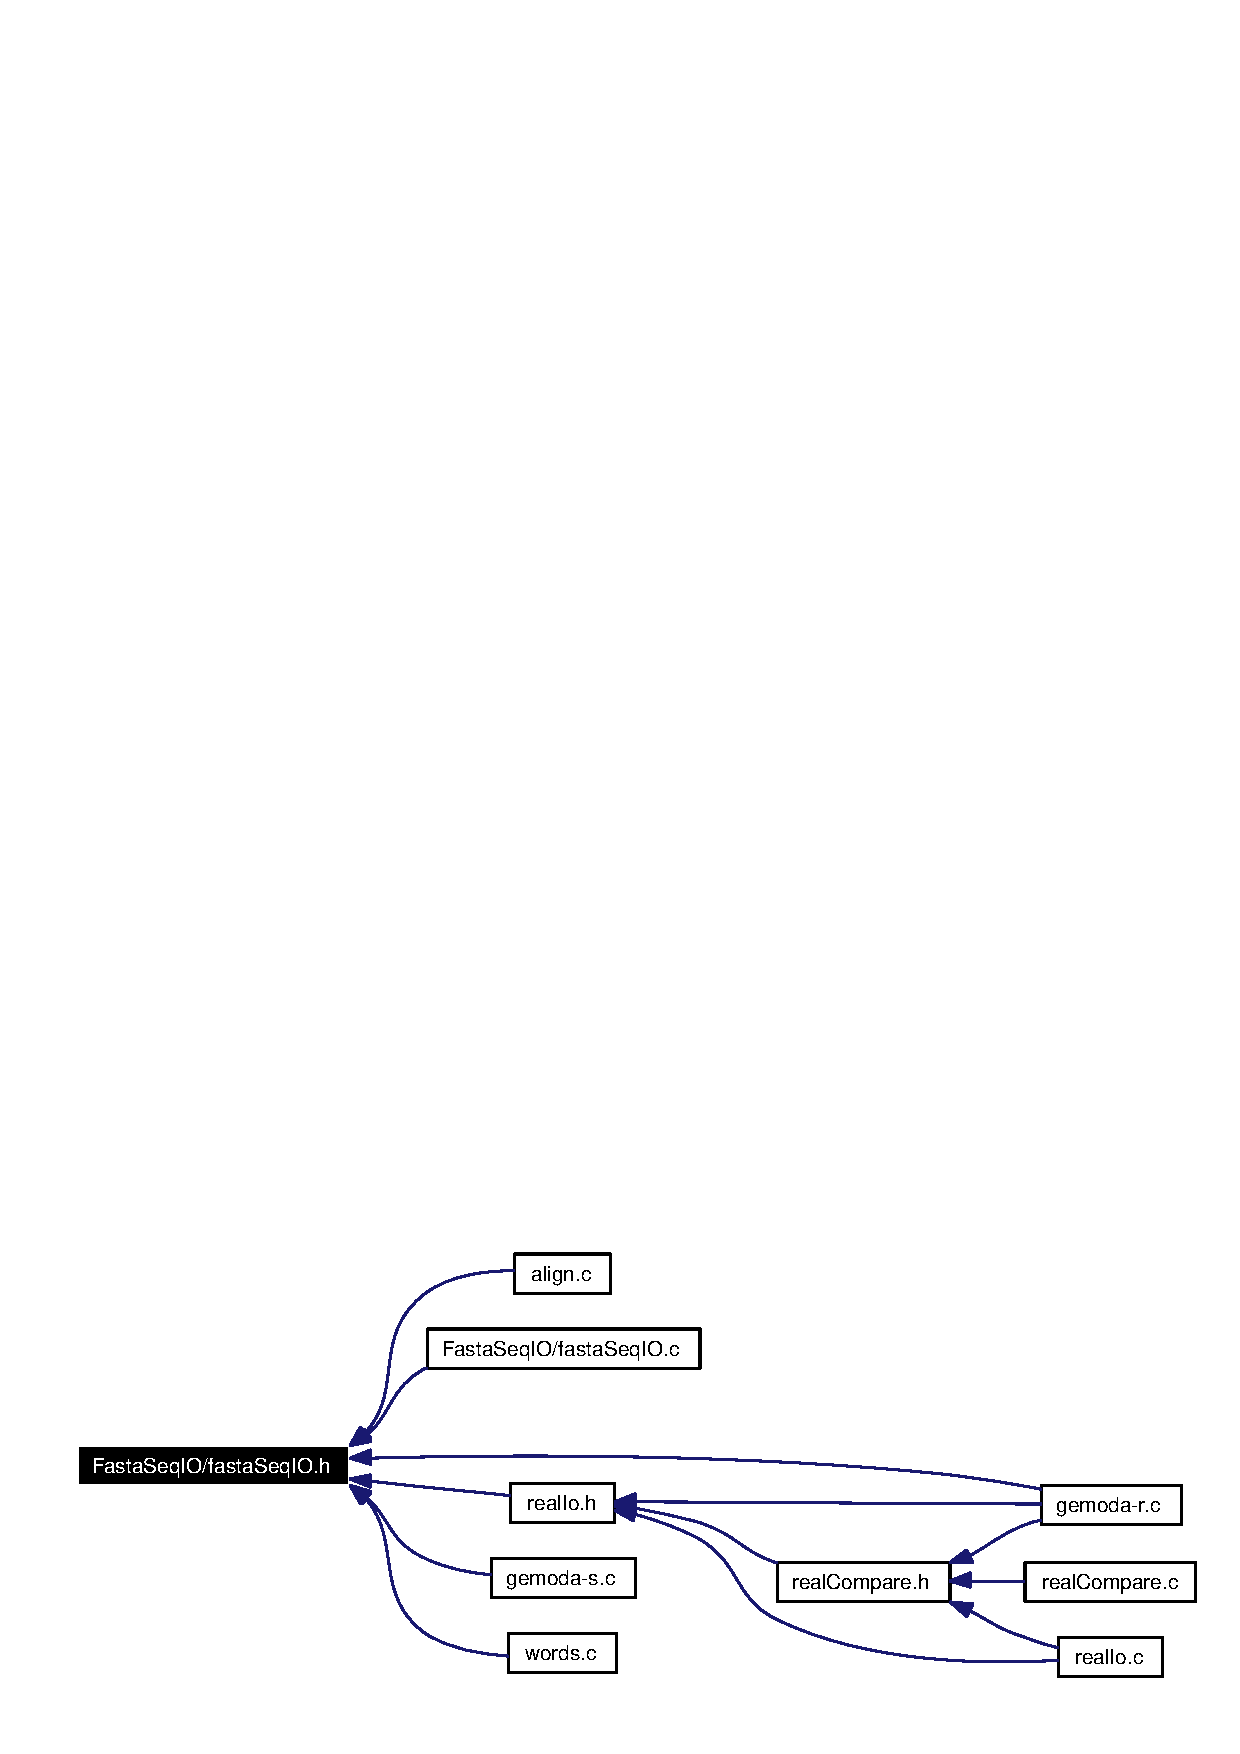
\includegraphics[width=287pt]{fastaSeqIO_8h__dep__incl}
\end{center}
\end{figure}
\subsection*{Data Structures}
\begin{CompactItemize}
\item 
struct \hyperlink{structfSeq__t}{f\-Seq\_\-t}
\end{CompactItemize}
\subsection*{Functions}
\begin{CompactItemize}
\item 
int \hyperlink{fastaSeqIO_8h_a0}{print\-FSeq\-Sub\-Seq} (\hyperlink{structfSeq__t}{f\-Seq\_\-t} $\ast$seq, int start, int stop)
\item 
long \hyperlink{fastaSeqIO_8h_a1}{measure\-Line} (FILE $\ast$INPUT)
\item 
long \hyperlink{fastaSeqIO_8h_a2}{count\-Lines} (FILE $\ast$INPUT)
\item 
long \hyperlink{fastaSeqIO_8h_a3}{Count\-FSeqs} (FILE $\ast$INPUT)
\item 
int \hyperlink{fastaSeqIO_8h_a4}{init\-Aof\-FSeqs} (\hyperlink{structfSeq__t}{f\-Seq\_\-t} $\ast$aos, int num\-Seq)
\item 
\hyperlink{structfSeq__t}{f\-Seq\_\-t} $\ast$ \hyperlink{fastaSeqIO_8h_a5}{Read\-FSeqs} (FILE $\ast$INPUT, int $\ast$number\-Of\-Sequences)
\item 
int \hyperlink{fastaSeqIO_8h_a6}{Free\-FSeqs} (\hyperlink{structfSeq__t}{f\-Seq\_\-t} $\ast$array\-Of\-Sequences, int number\-Of\-Sequences)
\item 
int \hyperlink{fastaSeqIO_8h_a7}{Write\-FSeq\-A} (FILE $\ast$MY\_\-FILE, \hyperlink{structfSeq__t}{f\-Seq\_\-t} $\ast$array\-Of\-Sequences, int start, int stop)
\item 
\hyperlink{structfSeq__t}{f\-Seq\_\-t} $\ast$ \hyperlink{fastaSeqIO_8h_a8}{Read\-Txt\-Seqs} (FILE $\ast$INPUT, int $\ast$number\-Of\-Sequences)
\end{CompactItemize}


\subsection*{Function Documentation}
\hypertarget{fastaSeqIO_8h_a3}{
\index{fastaSeqIO.h@{fasta\-Seq\-IO.h}!CountFSeqs@{CountFSeqs}}
\index{CountFSeqs@{CountFSeqs}!fastaSeqIO.h@{fasta\-Seq\-IO.h}}
\subsubsection[CountFSeqs]{\setlength{\rightskip}{0pt plus 5cm}long Count\-FSeqs (FILE $\ast$ {\em INPUT})}}
\label{fastaSeqIO_8h_a3}




Definition at line 44 of file fasta\-Seq\-IO.c.



\hypertarget{fastaSeqIO_8h_a2}{
\index{fastaSeqIO.h@{fasta\-Seq\-IO.h}!countLines@{countLines}}
\index{countLines@{countLines}!fastaSeqIO.h@{fasta\-Seq\-IO.h}}
\subsubsection[countLines]{\setlength{\rightskip}{0pt plus 5cm}long count\-Lines (FILE $\ast$ {\em INPUT})}}
\label{fastaSeqIO_8h_a2}




Definition at line 69 of file fasta\-Seq\-IO.c.

Referenced by Read\-File().



\hypertarget{fastaSeqIO_8h_a6}{
\index{fastaSeqIO.h@{fasta\-Seq\-IO.h}!FreeFSeqs@{FreeFSeqs}}
\index{FreeFSeqs@{FreeFSeqs}!fastaSeqIO.h@{fasta\-Seq\-IO.h}}
\subsubsection[FreeFSeqs]{\setlength{\rightskip}{0pt plus 5cm}int Free\-FSeqs (\hyperlink{structfSeq__t}{f\-Seq\_\-t} $\ast$ {\em array\-Of\-Sequences}, int {\em number\-Of\-Sequences})}}
\label{fastaSeqIO_8h_a6}




Definition at line 306 of file fasta\-Seq\-IO.c.

References f\-Seq\_\-t::label, and f\-Seq\_\-t::seq.

Referenced by main().



\hypertarget{fastaSeqIO_8h_a4}{
\index{fastaSeqIO.h@{fasta\-Seq\-IO.h}!initAofFSeqs@{initAofFSeqs}}
\index{initAofFSeqs@{initAofFSeqs}!fastaSeqIO.h@{fasta\-Seq\-IO.h}}
\subsubsection[initAofFSeqs]{\setlength{\rightskip}{0pt plus 5cm}int init\-Aof\-FSeqs (\hyperlink{structfSeq__t}{f\-Seq\_\-t} $\ast$ {\em aos}, int {\em num\-Seq})}}
\label{fastaSeqIO_8h_a4}




Definition at line 94 of file fasta\-Seq\-IO.c.

References f\-Seq\_\-t::label, and f\-Seq\_\-t::seq.

Referenced by Read\-FSeqs(), and Read\-Txt\-Seqs().



\hypertarget{fastaSeqIO_8h_a1}{
\index{fastaSeqIO.h@{fasta\-Seq\-IO.h}!measureLine@{measureLine}}
\index{measureLine@{measureLine}!fastaSeqIO.h@{fasta\-Seq\-IO.h}}
\subsubsection[measureLine]{\setlength{\rightskip}{0pt plus 5cm}long measure\-Line (FILE $\ast$ {\em INPUT})}}
\label{fastaSeqIO_8h_a1}




Definition at line 25 of file fasta\-Seq\-IO.c.

Referenced by Read\-File().



\hypertarget{fastaSeqIO_8h_a0}{
\index{fastaSeqIO.h@{fasta\-Seq\-IO.h}!printFSeqSubSeq@{printFSeqSubSeq}}
\index{printFSeqSubSeq@{printFSeqSubSeq}!fastaSeqIO.h@{fasta\-Seq\-IO.h}}
\subsubsection[printFSeqSubSeq]{\setlength{\rightskip}{0pt plus 5cm}int print\-FSeq\-Sub\-Seq (\hyperlink{structfSeq__t}{f\-Seq\_\-t} $\ast$ {\em seq}, int {\em start}, int {\em stop})}}
\label{fastaSeqIO_8h_a0}




Definition at line 14 of file fasta\-Seq\-IO.c.

References f\-Seq\_\-t::seq.



\hypertarget{fastaSeqIO_8h_a5}{
\index{fastaSeqIO.h@{fasta\-Seq\-IO.h}!ReadFSeqs@{ReadFSeqs}}
\index{ReadFSeqs@{ReadFSeqs}!fastaSeqIO.h@{fasta\-Seq\-IO.h}}
\subsubsection[ReadFSeqs]{\setlength{\rightskip}{0pt plus 5cm}\hyperlink{structfSeq__t}{f\-Seq\_\-t}$\ast$ Read\-FSeqs (FILE $\ast$ {\em INPUT}, int $\ast$ {\em number\-Of\-Sequences})}}
\label{fastaSeqIO_8h_a5}




Definition at line 199 of file fasta\-Seq\-IO.c.

References init\-Aof\-FSeqs(), f\-Seq\_\-t::label, Read\-File(), f\-Seq\_\-t::seq, s\-Size\_\-t::size, s\-Size\_\-t::start, and s\-Size\_\-t::stop.

Referenced by main().



\hypertarget{fastaSeqIO_8h_a8}{
\index{fastaSeqIO.h@{fasta\-Seq\-IO.h}!ReadTxtSeqs@{ReadTxtSeqs}}
\index{ReadTxtSeqs@{ReadTxtSeqs}!fastaSeqIO.h@{fasta\-Seq\-IO.h}}
\subsubsection[ReadTxtSeqs]{\setlength{\rightskip}{0pt plus 5cm}\hyperlink{structfSeq__t}{f\-Seq\_\-t}$\ast$ Read\-Txt\-Seqs (FILE $\ast$ {\em INPUT}, int $\ast$ {\em number\-Of\-Sequences})}}
\label{fastaSeqIO_8h_a8}




Definition at line 172 of file fasta\-Seq\-IO.c.

References init\-Aof\-FSeqs(), Read\-File(), and f\-Seq\_\-t::seq.



\hypertarget{fastaSeqIO_8h_a7}{
\index{fastaSeqIO.h@{fasta\-Seq\-IO.h}!WriteFSeqA@{WriteFSeqA}}
\index{WriteFSeqA@{WriteFSeqA}!fastaSeqIO.h@{fasta\-Seq\-IO.h}}
\subsubsection[WriteFSeqA]{\setlength{\rightskip}{0pt plus 5cm}int Write\-FSeq\-A (FILE $\ast$ {\em MY\_\-FILE}, \hyperlink{structfSeq__t}{f\-Seq\_\-t} $\ast$ {\em array\-Of\-Sequences}, int {\em start}, int {\em stop})}}
\label{fastaSeqIO_8h_a7}




Definition at line 332 of file fasta\-Seq\-IO.c.




\hypertarget{gemoda-r_8c}{
\section{gemoda-r.c File Reference}
\label{gemoda-r_8c}\index{gemoda-r.c@{gemoda-r.c}}
}
{\tt \#include \char`\"{}bit\-Set.h\char`\"{}}\par
{\tt \#include \char`\"{}convll.h\char`\"{}}\par
{\tt \#include \char`\"{}Fasta\-Seq\-IO/fasta\-Seq\-IO.h\char`\"{}}\par
{\tt \#include $<$unistd.h$>$}\par
{\tt \#include $<$stdlib.h$>$}\par
{\tt \#include $<$errno.h$>$}\par
{\tt \#include $<$string.h$>$}\par
{\tt \#include \char`\"{}real\-Io.h\char`\"{}}\par
{\tt \#include \char`\"{}real\-Compare.h\char`\"{}}\par


Include dependency graph for gemoda-r.c:\begin{figure}[H]
\begin{center}
\leavevmode
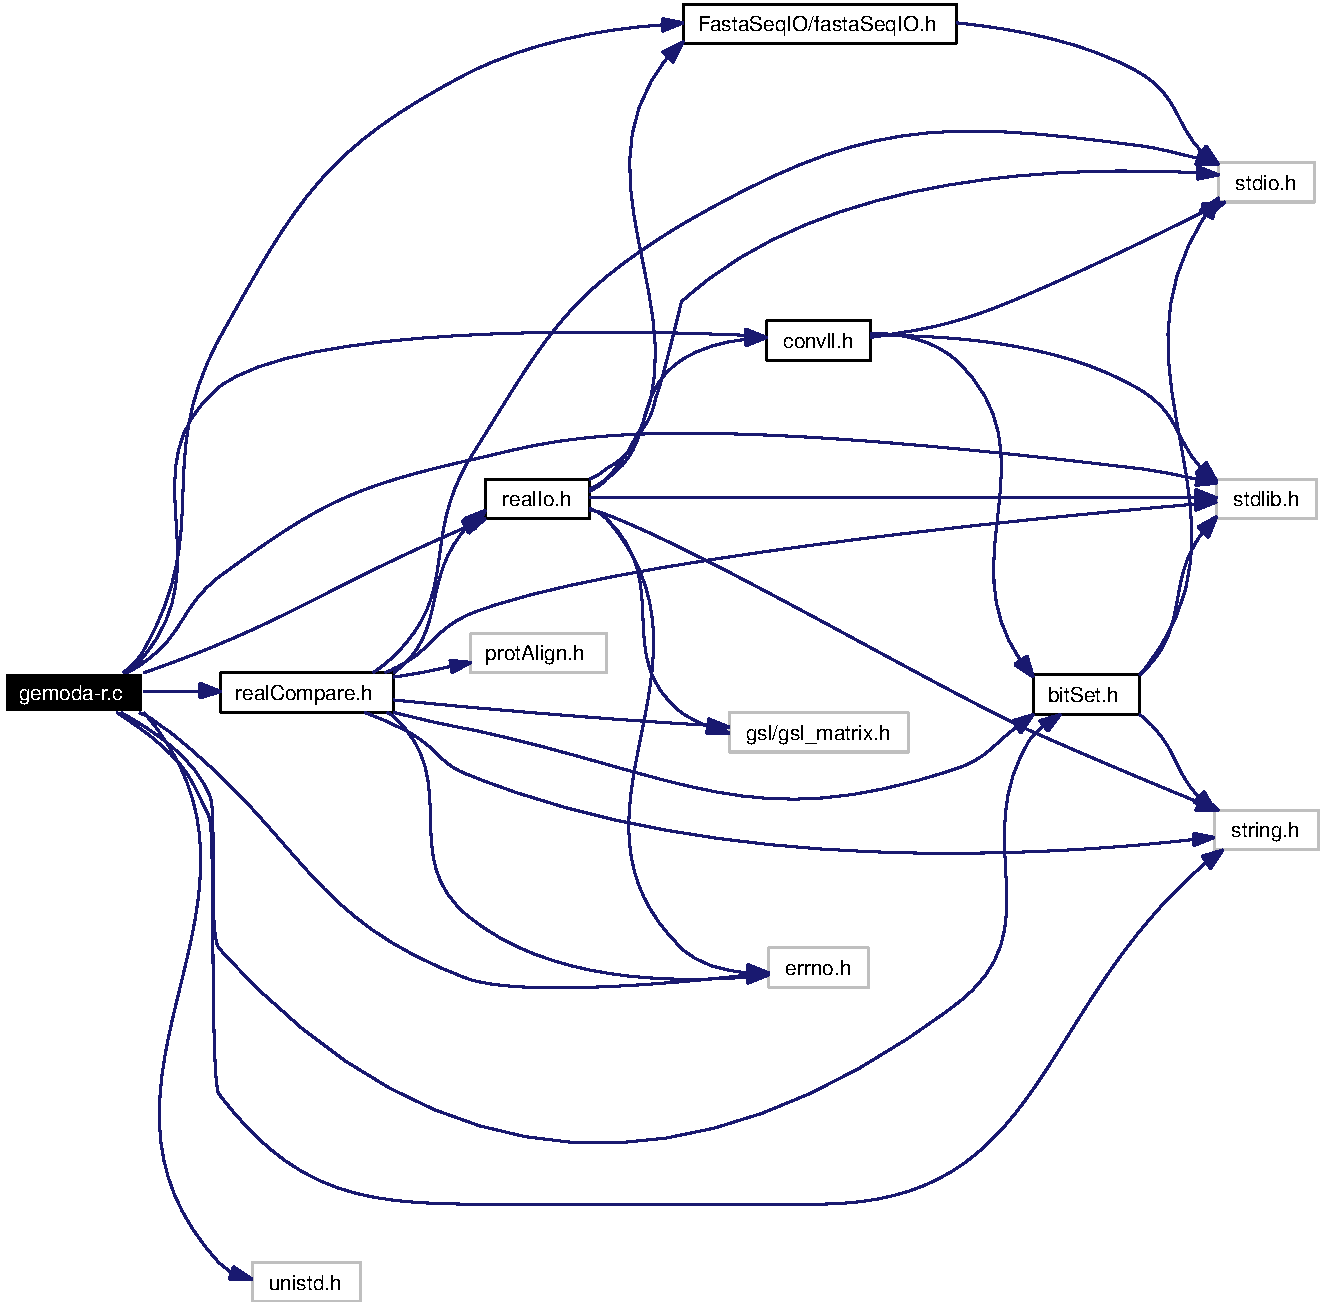
\includegraphics[width=334pt]{gemoda-r_8c__incl}
\end{center}
\end{figure}
\subsection*{Functions}
\begin{CompactItemize}
\item 
void \hyperlink{gemoda-r_8c_a0}{usage} (char $\ast$$\ast$argv)
\item 
\hyperlink{structcnode}{cll\_\-t} $\ast$ \hyperlink{gemoda-r_8c_a1}{convolve} (\hyperlink{structbitGraph__t}{bit\-Graph\_\-t} $\ast$bg, int support, int R, int $\ast$index\-To\-Seq, int p, int cluster\-Method, int $\ast$$\ast$offset\-To\-Index, int number\-Of\-Sequences, int no\-Convolve, FILE $\ast$OUTPUT\_\-FILE)
\item 
\hyperlink{structbitGraph__t}{bit\-Graph\_\-t} $\ast$ \hyperlink{gemoda-r_8c_a2}{prune\-Bit\-Graph} (\hyperlink{structbitGraph__t}{bit\-Graph\_\-t} $\ast$bg, int $\ast$index\-To\-Seq, int $\ast$$\ast$offset\-To\-Index, int num\-Of\-Seqs, int p)
\item 
int \hyperlink{gemoda-r_8c_a3}{count\-Extra\-Params} (char $\ast$s)
\item 
double $\ast$ \hyperlink{gemoda-r_8c_a4}{parse\-Extra\-Params} (char $\ast$s, int num\-Params)
\item 
int \hyperlink{gemoda-r_8c_a5}{main} (int argc, char $\ast$$\ast$argv)
\end{CompactItemize}


\subsection*{Detailed Description}
This file contains the main routine for the real valued version of Gemoda. There are also some accessory functions for printing information on how to use Gemoda and run it from the commandline.

Definition in file \hyperlink{gemoda-r_8c-source}{gemoda-r.c}.

\subsection*{Function Documentation}
\hypertarget{gemoda-r_8c_a1}{
\index{gemoda-r.c@{gemoda-r.c}!convolve@{convolve}}
\index{convolve@{convolve}!gemoda-r.c@{gemoda-r.c}}
\subsubsection[convolve]{\setlength{\rightskip}{0pt plus 5cm}\hyperlink{structcnode}{cll\_\-t}$\ast$ convolve (\hyperlink{structbitGraph__t}{bit\-Graph\_\-t} $\ast$ {\em bg}, int {\em support}, int {\em R}, int $\ast$ {\em index\-To\-Seq}, int {\em p}, int {\em cluster\-Method}, int $\ast$$\ast$ {\em offset\-To\-Index}, int {\em number\-Of\-Sequences}, int {\em no\-Convolve}, FILE $\ast$ {\em OUTPUT\_\-FILE})}}
\label{gemoda-r_8c_a1}


Our outer convolution function. This function will call preliminary functions, cluster the data, and then call the main convolution function. This is the interface between the main gemoda-$<$x$>$ code and the generic code that gets all of the work done. Input: the bit\-Graph to be clustered and convolved, the minimum support necessary for a motif to be returned, a flag indicating whether recursive filtering should be used, a pointer to the data structure that dereferences offset indices to sequence numbers, the number of unique source sequences that a motif must be present in, and a number indicating the clustering method that is to be used. Output: the final motif linked list with all motifs that are to be given as output to the user.

Definition at line 625 of file new\-Conv.c.

Referenced by main().

\scriptsize\begin{verbatim}629 {
630   bitSet_t * cand = NULL;
631   bitSet_t * mask = NULL;
632   bitSet_t * Q = NULL;
633   int size = bg->size;
634   cll_t * elemPats = NULL;
635   cll_t * allCliques = NULL;
636   cll_t * curr = NULL;
637   
638     // contains indices (rows) containing the threshold value.
639     cand = newBitSet (size);
640   mask = newBitSet (size);
641   Q = newBitSet (size);
642   fillSet (cand);
643   fillSet (mask);
644   
645     // Note that we prune based on p before setting the diagonal false.
646     if (p > 1)
647     {
648       bg =
649     pruneBitGraph (bg, indexToSeq, offsetToIndex, numberOfSequences, p);
650     }
651   
652     // Now we set the main diagonal false for clustering and filtering.
653     bitGraphSetFalseDiagonal (bg);
654   filterGraph (bg, support, R);
655   fprintf (OUTPUT_FILE, "Graph filtered!  Now clustering...\n");
656   fflush (NULL);
657   if (clusterMethod == 0)
658     {
659       findCliques (Q, cand, mask, bg, support, 0, &elemPats, indexToSeq, p);
660     }
661   else
662     {
663       singleLinkage (Q, cand, mask, bg, support, 0, &elemPats, indexToSeq,
664               p);
665     }
666   fprintf (OUTPUT_FILE,
667         "Clusters found!  Now filtering clusters (if option set)...\n");
668   fflush (NULL);
669   if (p > 1)
670     {
671       elemPats = pruneCll (elemPats, indexToSeq, p);
672     }
673   deleteBitSet (cand);
674   deleteBitSet (mask);
675   deleteBitSet (Q);
676   
677     // Now let's convolve what we made.
678     if (noConvolve == 0)
679     {
680       fprintf (OUTPUT_FILE, "Now convolving...\n");
681       fflush (NULL);
682       allCliques = completeConv (&elemPats, support, size, 0, indexToSeq, p);
683     }
684   
685   else
686     {
687       curr = elemPats;
688       while (curr != NULL)
689     {
690       yankCll (&elemPats, NULL, &curr, &allCliques, 0);
691     }
692     }
693   return allCliques;
694 }
\end{verbatim}
\normalsize 


\hypertarget{gemoda-r_8c_a3}{
\index{gemoda-r.c@{gemoda-r.c}!countExtraParams@{countExtraParams}}
\index{countExtraParams@{countExtraParams}!gemoda-r.c@{gemoda-r.c}}
\subsubsection[countExtraParams]{\setlength{\rightskip}{0pt plus 5cm}int count\-Extra\-Params (char $\ast$ {\em s})}}
\label{gemoda-r_8c_a3}




Definition at line 91 of file gemoda-r.c.

Referenced by main().

\scriptsize\begin{verbatim}92 {
93   int i = 0;
94   int numParams = 1;
95   for (i = 0; i < strlen (s); i++)
96     {
97       if (s[i] == ',')
98     {
99       numParams++;
100     }
101     }
102   return numParams;
103 }
\end{verbatim}
\normalsize 


\hypertarget{gemoda-r_8c_a5}{
\index{gemoda-r.c@{gemoda-r.c}!main@{main}}
\index{main@{main}!gemoda-r.c@{gemoda-r.c}}
\subsubsection[main]{\setlength{\rightskip}{0pt plus 5cm}int main (int {\em argc}, char $\ast$$\ast$ {\em argv})}}
\label{gemoda-r_8c_a5}


This is the main routine of the real value Gemoda code. The code runs similarly to the sequence Gemoda code: there is a comparison phase, followed by a clustering phase, followed by a convolution phase. Only the comparison phase is unique to the real value Gemoda. Of course, since the data are formatted so differently, there are vastly different pieces of code in the front matter. In particular, there is no hashing of words obviously. As well, we use the GNU scientific library to store real value data as matrices that can be easily manipulated.

Definition at line 160 of file gemoda-r.c.

References calc\-Stat\-All\-Cliqs(), convolve(), count\-Extra\-Params(), cum\-DMatrix(), delete\-Bit\-Graph(), free\-D(), free\-Rdh(), get\-Stat\-Mat(), rdh\_\-t::index\-To\-Seq, rdh\_\-t::offset\-To\-Index, output\-Real\-Pats(), output\-Real\-Pats\-WCentroid(), parse\-Extra\-Params(), pop\-All\-Cll(), read\-Real\-Data(), real\-Comparison(), bit\-Graph\_\-t::size, rdh\_\-t::size, sort\-By\-Stats(), and usage().

\scriptsize\begin{verbatim}161 {
162   int inputOption = 0;
163   char *sequenceFile = NULL;
164   FILE *SEQUENCE_FILE = NULL;
165   char *outputFile = NULL;
166   FILE *OUTPUT_FILE = NULL;
167   int L = 0;
168   int status = 0;
169   double g = 0;
170   int sup = 2;
171   int R = 1;
172   int P = 0;
173   int compFunc = 0;
174   double *extraParams = NULL;
175   int numExtraParams = 0;
176   int i = 0, j = 0;
177   /*
178      int j, k, i, l;
179    */
180   int noConvolve = 0;
181   int samp = 1;
182   int supportDim = 0, lengthDim = 0;
183   bitGraph_t *oam = NULL;
184   unsigned int **d = NULL;
185   int oamSize = 0;
186 
187   cll_t *allCliques = NULL;
188   /*
189      cll_t *curCliq = NULL;
190    */
191   /*
192      int curSeq;
193    */
194   /*
195      int curPos;
196    */
197   int clusterMethod = 0;
198   int joelOutput = 0;
199 
200   // gemoda-r new stuff
201   rdh_t *data = NULL;
202 
203   /*
204      Get command-line options 
205    */
206   while ((inputOption = getopt (argc, argv, "p:m:e:i:o:l:g:k:c:njs:")) != EOF)
207     {
208       switch (inputOption)
209     {
210       // Comparison metric
211     case 'm':
212       compFunc = atoi (optarg);
213       break;
214       // Input file
215     case 'i':
216       sequenceFile = optarg;
217       break;
218       // Output file
219     case 'o':
220       outputFile =
221         (char *) malloc ((strlen (optarg) + 1) * sizeof (char));
222       if (outputFile == NULL)
223         {
224           fprintf (stderr, "Error allocating memory for options.\n");
225           exit (EXIT_FAILURE);
226         }
227       else
228         {
229           strcpy (outputFile, optarg);
230         }
231       break;
232       // Minimum motif length
233     case 'l':
234       L = atoi (optarg);
235       break;
236       // Minimum motif similarity score
237     case 'g':
238       g = atof (optarg);
239       status++;
240       break;
241       // Minimum support (number of motif occurrences)
242     case 'k':
243       sup = atoi (optarg);
244       break;
245 
246 /***************************************************************
247  * Recursive initial pruning: an option for clique finding.
248  *   It takes all nodes with less than the minimum
249  *   number of support and removes all of their nodes, and does this 
250  *   recursively so that nodes that are connected to many sparsely connected
251  *   nodes will be removed and not left in the 
252  * This option is deprecated as it is at worst no-gain and at best useful.
253  *   It will be on by default for clique-finding, but can be turned 
254  *   back off with some
255  *   minor tweaking.  For almost all cases in which it does not speed
256  *   up computations, it will have a trivial time to perform.  Thus, if 
257  *   clique-finding is turned on, then R is set to 1 by default.
258         case 'r':
259             R = 1;
260             break;
261 ************************************************************************/
262       // Optional pruning parameter to require at motif occurrences
263       // in at least P distinct input sequences
264 
265     case 'p':
266       P = atoi (optarg);
267       break;
268 
269       // Clustering method.
270     case 'c':
271       clusterMethod = atoi (optarg);
272       break;
273       // Extra parameters for comparison function
274     case 'e':
275       numExtraParams = countExtraParams (optarg);
276       extraParams = parseExtraParams (optarg, numExtraParams);
277       break;
278     case 'n':
279       noConvolve = 1;
280       break;
281     case 'j':
282       joelOutput = 1;
283       break;
284     case 's':
285       samp = atoi (optarg);
286       break;
287       // Catch-all.
288     case '?':
289       fprintf (stderr, "Unknown option `-%c'.\n", optopt);
290       usage (argv);
291       return EXIT_SUCCESS;
292     default:
293       usage (argv);
294       return EXIT_SUCCESS;
295     }
296     }
297   // Require an input file, a nonzero length, and a similarity threshold
298   // to be set.
299   if (sequenceFile == NULL || L == 0 || status < 1)
300     {
301       usage (argv);
302       return EXIT_SUCCESS;
303     }
304   // Open the sequence file
305   if ((SEQUENCE_FILE = fopen (sequenceFile, "r")) == NULL)
306     {
307       fprintf (stderr, "Couldn't open file %s; %s\n", sequenceFile,
308            strerror (errno));
309       exit (EXIT_FAILURE);
310     }
311   // Open the output file
312   if (outputFile != NULL)
313     {
314       if ((OUTPUT_FILE = fopen (outputFile, "w")) == NULL)
315     {
316       fprintf (stderr, "Couldn't open file %s; %s\n", outputFile,
317            strerror (errno));
318       exit (EXIT_FAILURE);
319     }
320     }
321   else
322     {
323       OUTPUT_FILE = stdout;
324     }
325 
326 
327 
328   // Verbosity in output helps to distinguish output files.
329   fprintf (OUTPUT_FILE, "Input file = %s\n", sequenceFile);
330   fprintf (OUTPUT_FILE, "l = %d, k = %d, g = %f\n", L, sup, g);
331   if (P > 1)
332     {
333       fprintf (OUTPUT_FILE, "Minimum # of sequences with motif = %d\n", P);
334     }
335   if (R > 0)
336     {
337       fprintf (OUTPUT_FILE, "Recursive pruning is ON.\n");
338     }
339 
340   data = readRealData (SEQUENCE_FILE);
341   fclose (SEQUENCE_FILE);
342   // printf("size = %d,indexSize = %d\n",data->size,data->indexSize);
343   // printf("size1 = %d,size2 = %d\n",data->seq[0]->size1,data->seq[0]->size2);
344   // for(i = 0; i < 2; i++) {
345   // for(j = 0; j < 3; j++) {
346   // printf("%lf,%lf,%lf\n",gsl_matrix_get(data->seq[i],j,0),
347   // gsl_matrix_get(data->seq[i],j,1),
348   // gsl_matrix_get(data->seq[i],j,2));}}
349   oam = realComparison (data, L, g, compFunc, extraParams);
350   // printf("oam->size = %d\n", oam->size);
351   if ((samp > 0) && (clusterMethod == 0))
352     {
353       // We are currently using one gap per sequence, as done in 
354       // realCompare.c's call to initRdhIndex in realComparison.
355       // Note that this is data->size, NOT oam->size.
356       d =
357     getStatMat (oam, sup, L, &supportDim, &lengthDim, data->size, samp,
358             OUTPUT_FILE);
359     }
360   else
361     {
362       d = NULL;
363       supportDim = 0;
364     }
365 
366   allCliques =
367     convolve (oam, sup, R, data->indexToSeq, P, clusterMethod,
368           data->offsetToIndex, data->size, noConvolve, OUTPUT_FILE);
369 
370   oamSize = oam->size;
371   // Do some early memory cleanup since this is so big.
372   deleteBitGraph (oam);
373 
374   if ((samp > 0) && (clusterMethod == 0))
375     {
376       cumDMatrix (d, allCliques, supportDim, lengthDim, oamSize, data->size);
377       calcStatAllCliqs (d, allCliques, oamSize - data->size);
378       allCliques = sortByStats (allCliques);
379     }
380 
381   if (joelOutput == 0)
382     {
383       outputRealPats (data, allCliques, L, OUTPUT_FILE, d);
384     }
385   else
386     {
387       outputRealPatsWCentroid (data, allCliques, L, OUTPUT_FILE, extraParams,
388                    compFunc);
389     }
390 
391   freeD (d, supportDim);
392   freeRdh (data);
393   allCliques = popAllCll (allCliques);
394   fclose (OUTPUT_FILE);
395 
396   return 0;
397 }
\end{verbatim}
\normalsize 


\hypertarget{gemoda-r_8c_a4}{
\index{gemoda-r.c@{gemoda-r.c}!parseExtraParams@{parseExtraParams}}
\index{parseExtraParams@{parseExtraParams}!gemoda-r.c@{gemoda-r.c}}
\subsubsection[parseExtraParams]{\setlength{\rightskip}{0pt plus 5cm}double$\ast$ parse\-Extra\-Params (char $\ast$ {\em s}, int {\em num\-Params})}}
\label{gemoda-r_8c_a4}


This was borrowed from the old gemoda-p code, there it used to parse filenames, here we are parsing comma-separated lists of doubles that are useful for Spec\-Connect.

Definition at line 110 of file gemoda-r.c.

Referenced by main().

\scriptsize\begin{verbatim}111 {
112   int i = 0, j = 0, k = 0;
113   int startLength = 0;
114   double *extraParams = NULL;
115   char *paramString = NULL;
116 
117   extraParams = (double *) malloc (numParams * sizeof (double));
118   if (extraParams == NULL)
119     {
120       fprintf (stderr, "Can't allocate extra params!\n");
121       exit (0);
122     }
123   j = 0;
124   k = 0;
125   startLength = strlen (s);
126   for (i = 0; i < startLength; i++)
127     {
128       if (s[i] == ',')
129     {
130       // We've found an end.  So point the pointer to
131       // the beginning of the previous string.
132       paramString = &s[k];
133       // Terminate the string where the comma used to be
134       s[i] = '\0';
135       // Update the location for the next string beginning
136       k = i + 1;
137       // Convert to a double and update the param number.
138       extraParams[j] = atof (paramString);
139       j++;
140     }
141     }
142   // Don't forget to do the last one, which isn't comma-terminated.
143   paramString = &s[k];
144   extraParams[j] = atof (paramString);
145   return (extraParams);
146 }
\end{verbatim}
\normalsize 


\hypertarget{gemoda-r_8c_a2}{
\index{gemoda-r.c@{gemoda-r.c}!pruneBitGraph@{pruneBitGraph}}
\index{pruneBitGraph@{pruneBitGraph}!gemoda-r.c@{gemoda-r.c}}
\subsubsection[pruneBitGraph]{\setlength{\rightskip}{0pt plus 5cm}\hyperlink{structbitGraph__t}{bit\-Graph\_\-t}$\ast$ prune\-Bit\-Graph (\hyperlink{structbitGraph__t}{bit\-Graph\_\-t} $\ast$ {\em bg}, int $\ast$ {\em index\-To\-Seq}, int $\ast$$\ast$ {\em offset\-To\-Index}, int {\em num\-Of\-Seqs}, int {\em p})}}
\label{gemoda-r_8c_a2}


Simple function (non-recursive) to prune off the first level of motifs that will not meet the \char`\"{}minimum number of unique sequences\char`\"{} criterion. This could have been implemented as above, but it may have gotten a little expensive with less yield, so only the first run through is done here. Input: a bit graph to be pruned, a pointer to the structure that dereferences offset indices to sequence numbers, a pointer to the structure that dereferences seq/position to offsets, the number of unique sequences in the input set, and the minimum number of unique sequences that must contain the motif. Output: a pruned bit\-Graph.

Definition at line 402 of file new\-Conv.c.

Referenced by convolve().

\scriptsize\begin{verbatim}404 {
405   int i = 0, j = 0, nextBit = 0;
406   int *seqNums = NULL;
407   
408     // Since we don't immediately know which node is in which source 
409     // sequence, we can't just count them up regularly.  Instead, we'll
410     // need to keep track of which sequences they come from and 
411     // increment _something_.  What we chose to do here is just make
412     // an array of integers of length = <p>.  Then, we try to put the
413     // source sequence number of each neighbor (including itself, since
414     // the main diagonal is still true at this time) into the next slot
415     // Since we will monotonically search the bitSet, we can just 
416     // move on to the first bit in the next sequence using the 
417     // offsetToIndex structure so that we know the next sequence number
418     // to be put in is always unique.
419     seqNums = (int *) malloc (p * sizeof (int));
420   if (seqNums == NULL)
421     {
422       fprintf (stderr, "Memory error - pruneBitGraph\n%s\n",
423         strerror (errno));
424       fflush (stderr);
425       exit (0);
426     }
427   
428     // So, for each row in the bitgraph...
429     for (i = 0; i < bg->size; i++)
430     {
431       
432     // Make sure the whole array is -1 sentinels.
433     for (j = 0; j < p; j++)
434     {
435       seqNums[j] = -1;
436     }
437       j = 0;
438       
439     // Find the first neighbor of this bit.
440     nextBit = nextBitBitSet (bg->graph[i], 0);
441       if (nextBit == -1)
442     {
443       continue;
444     }
445       else
446     {
447       
448         // and put its sequence number in the array of ints.
449         seqNums[0] = indexToSeq[nextBit];
450     }
451       
452     // If it's the last sequence, then bail out so that we don't
453     // segfault in the next step.
454     if (seqNums[0] >= numOfSeqs - 1)
455     {
456       emptySet (bg->graph[i]);
457       continue;
458     }
459       
460     // Find the next neighbor of this bit, STARTING AT the first
461     // bit in the next sequence.
462     nextBit =
463     nextBitBitSet (bg->graph[i],
464                offsetToIndex[indexToSeq[nextBit] + 1][0]);
465       
466     // And iterate this until we run out of neighbors.
467     while (nextBit >= 0)
468     {
469       j++;
470       seqNums[j] = indexToSeq[nextBit];
471       
472         // Or until this new neighbor will fill up the array
473         if (j == p - 1)
474         {
475           break;
476         }
477       
478         // Or until this new neighbor is in the last sequence.
479         if (seqNums[j] >= numOfSeqs - 1)
480         {
481           break;
482         }
483       
484         // Get the next neighbor!
485         nextBit =
486         nextBitBitSet (bg->graph[i],
487                offsetToIndex[indexToSeq[nextBit] + 1][0]);
488     }
489       
490     // If we didn't have enough unique sequences, and either a) we
491     // were in the nth-to-last sequence and there were no 
492     // neighbors after it, or b) we were in the last sequence,
493     // then the last number will still be our sentinel, -1.  If
494     // the last number is not a sentinel, then we have at least
495     // p distinct sequence occurrences, so we're OK.
496     if (seqNums[p - 1] == -1)
497     {
498       emptySet (bg->graph[i]);
499     }
500     }
501   free (seqNums);
502   return (bg);
503 }
\end{verbatim}
\normalsize 


\hypertarget{gemoda-r_8c_a0}{
\index{gemoda-r.c@{gemoda-r.c}!usage@{usage}}
\index{usage@{usage}!gemoda-r.c@{gemoda-r.c}}
\subsubsection[usage]{\setlength{\rightskip}{0pt plus 5cm}void usage (char $\ast$$\ast$ {\em argv})}}
\label{gemoda-r_8c_a0}


This function tells the user how to run Gemoda. The function displays all the available flags and gives an example of how to use the commandline to run the code.

Definition at line 35 of file gemoda-r.c.

Referenced by main().

\scriptsize\begin{verbatim}36 {
37   fprintf (stdout,
38        "Usage: %s -i <Fasta sequence file> "
39        "-l <word size> \n\t-k <support> -g <threshold> "
	  "-m <matrix name> [-z] \n\t[-c <cluster method [0|1]>]"
	  "[-p <unique support>] \n\n\n"
40        "Required flags and input:\n\n"
41        "-i <Fasta sequence file>:\n\t"
42        "File containing all sequences to be searched, in Fasta format.\n\n"
43        "-l <word size>:\n\t"
44        "Minimum length of motifs; also the sliding window length\n\t"
45        "over which all motifs must meet the similarity criterion\n\n"
46        "-k <support>:\n\t"
47        "Minimum number of motif occurrences.\n\n"
48        "-g <threshold>:\n\t"
49        "Similarity threshold.  Two windows, when scored with the\n\t"
50        " similarity matrix defined by the -m flag, must have at least\n\t"
51        " this score in order to be deemed 'connected'.  This criterion\n\t"
52        " must be met over all sliding windows of length l.\n\n"
53        "-c <cluster method [0|1]>:\n\t"
54        "The clustering method to be used after evaluating the "
55        "\n\tsimilarity of the unique words in the input.  Note that the "
56        "\n\tclustering method will have a significant impact on both the "
57        "\n\tresults that one obtains and the computation time.\n\n\t"
58        "0: clique-finding\n\t\t"
59        "Uses established methods to find all maximal cliques in the "
60        "\n\t\tdata.  This will give the most thorough results (that are "
61        "\n\t\tprovably exhaustive), but will also give less-significant "
62        "\n\t\tresults in addition to the most interesting and most\n\t"
63        "significant ones.  The results are deterministic but may take some "
64        "\n\t\ttime on data sets with high similarity or if the similarity "
65        "\n\t\tthreshold is set extremely low.\n\t"
66        "1: single-linkage clustering\n\t\t"
67        "Uses a single-linkage-type clustering where all nodes that "
68        "\n\t\tare connected are put in the same cluster.  This method is "
69        "\n\t\talso deterministic and will be faster than clique-finding, "
70        "\n\t\tbut it loses guarantees of exhaustiveness in searching the "
71        "\n\t\tdata set.\n\n",
72        "-p <unique support>:\n\t"
73        "A pruning parameter that requires the motif to occur in "
74        "\n\tat least <unique support> different input sequences.  Note "
75        "\n\tthat this parameter must be less than or equal to the total "
76        "\n\tsupport parameter set by the -k flag.\n\n", argv[0]);
77   fprintf (stdout, "\n");
78 }
\end{verbatim}
\normalsize 



\hypertarget{gemoda-s_8c}{
\section{gemoda-s.c File Reference}
\label{gemoda-s_8c}\index{gemoda-s.c@{gemoda-s.c}}
}
{\tt \#include \char`\"{}bit\-Set.h\char`\"{}}\par
{\tt \#include \char`\"{}spat.h\char`\"{}}\par
{\tt \#include \char`\"{}convll.h\char`\"{}}\par
{\tt \#include \char`\"{}matdata.h\char`\"{}}\par
{\tt \#include \char`\"{}Fasta\-Seq\-IO/fasta\-Seq\-IO.h\char`\"{}}\par
{\tt \#include $<$unistd.h$>$}\par
{\tt \#include $<$stdlib.h$>$}\par
{\tt \#include $<$errno.h$>$}\par
{\tt \#include $<$string.h$>$}\par
{\tt \#include \char`\"{}pat\-Stats.h\char`\"{}}\par


Include dependency graph for gemoda-s.c:\begin{figure}[H]
\begin{center}
\leavevmode
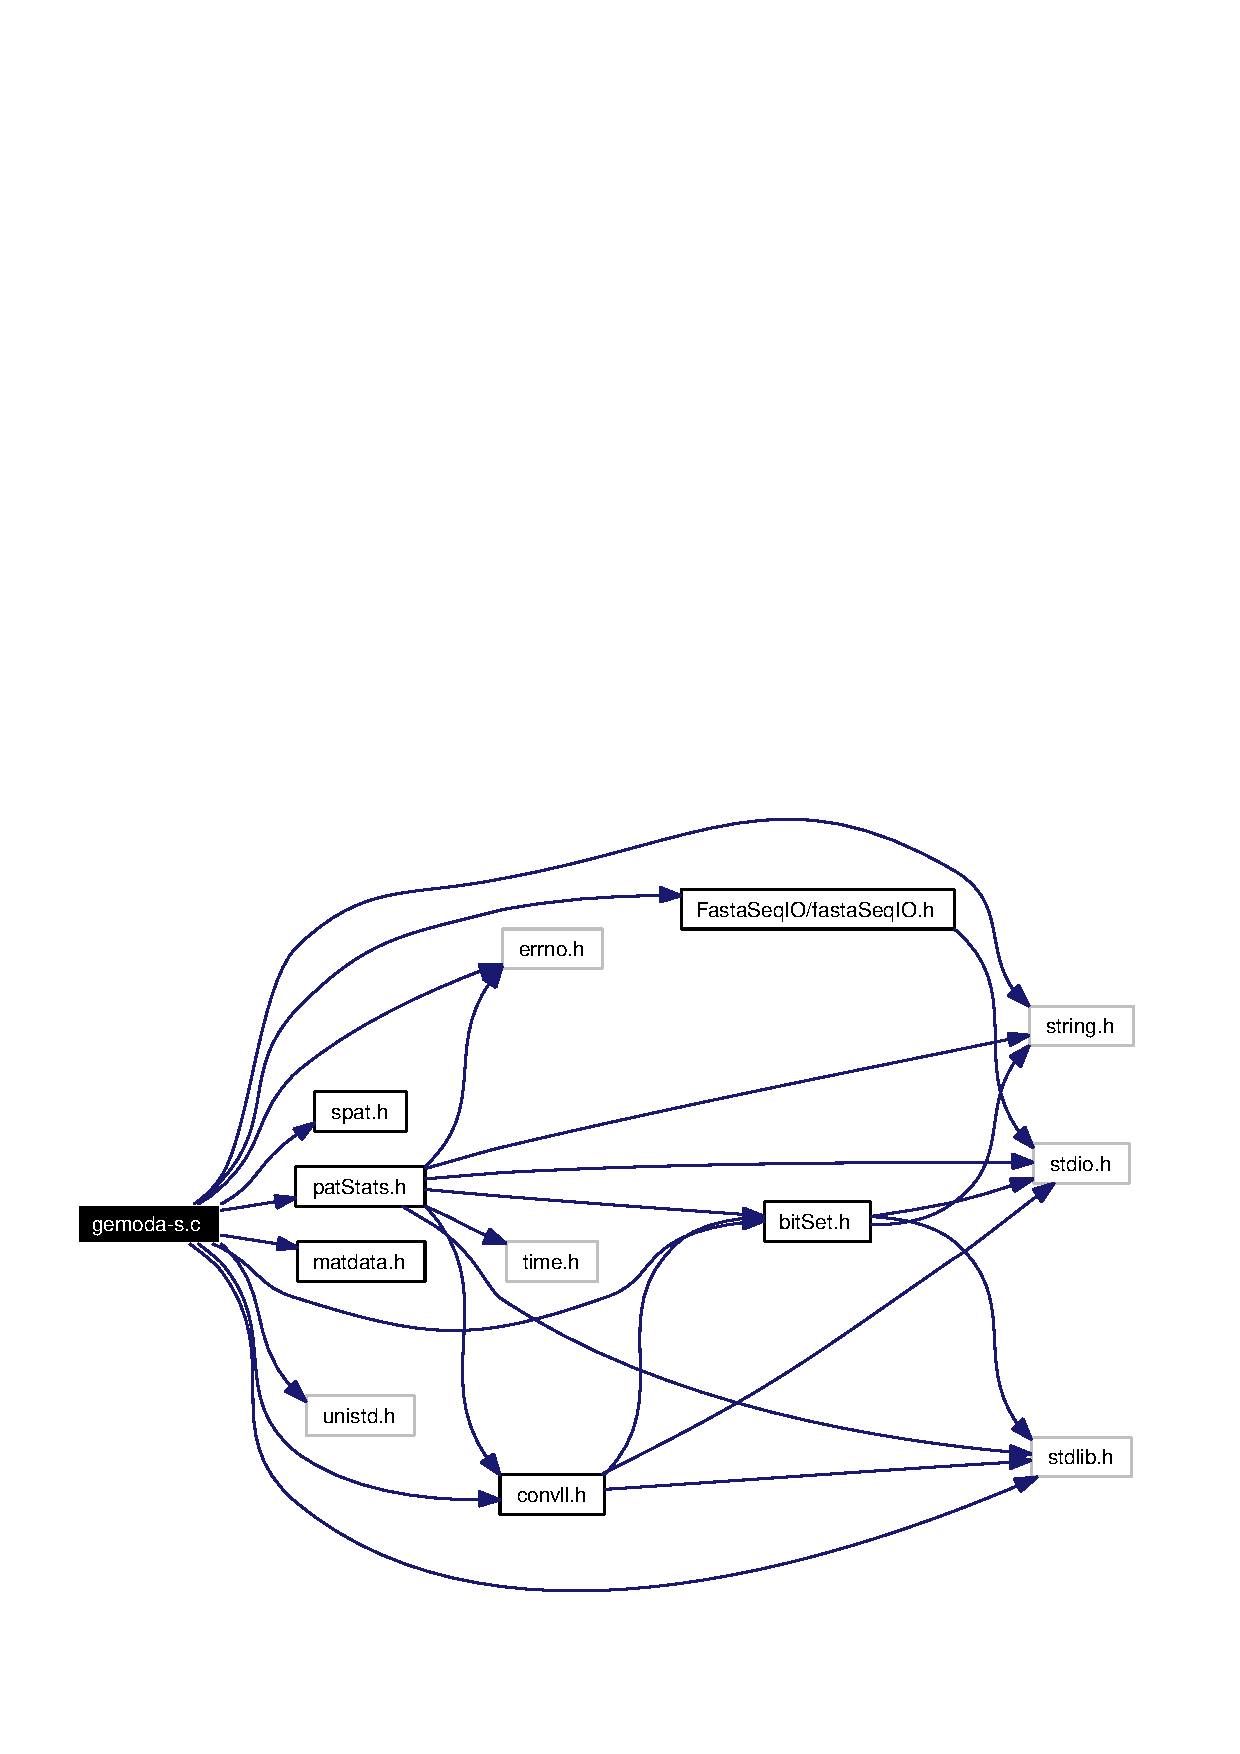
\includegraphics[width=272pt]{gemoda-s_8c__incl}
\end{center}
\end{figure}
\subsection*{Functions}
\begin{CompactItemize}
\item 
void \hyperlink{gemoda-s_8c_a0}{usage} (char $\ast$$\ast$argv)
\item 
void \hyperlink{gemoda-s_8c_a1}{matrixlist} (void)
\item 
void \hyperlink{gemoda-s_8c_a2}{get\-Matrix\-By\-Name} (char \hyperlink{matrixmap_8h_a0}{name}\mbox{[}$\,$\mbox{]}, int \hyperlink{matrixmap_8h_a1}{mat}\mbox{[}$\,$\mbox{]}\mbox{[}MATRIX\_\-SIZE\mbox{]})
\item 
\hyperlink{structbitGraph__t}{bit\-Graph\_\-t} $\ast$ \hyperlink{gemoda-s_8c_a3}{align\-Words\-Mat\_\-bit} (\hyperlink{structsPat__t}{s\-Pat\_\-t} $\ast$words, int wc, int \hyperlink{matrixmap_8h_a1}{mat}\mbox{[}$\,$\mbox{]}\mbox{[}MATRIX\_\-SIZE\mbox{]}, int threshold)
\item 
\hyperlink{structsPat__t}{s\-Pat\_\-t} $\ast$ \hyperlink{gemoda-s_8c_a4}{count\-Words2} (\hyperlink{structfSeq__t}{f\-Seq\_\-t} $\ast$seq, int num\-Seq, int L, int $\ast$num\-Words)
\item 
\hyperlink{structcnode}{cll\_\-t} $\ast$ \hyperlink{gemoda-s_8c_a5}{convolve} (\hyperlink{structbitGraph__t}{bit\-Graph\_\-t} $\ast$bg, int support, int R, int $\ast$index\-To\-Seq, int p, int cluster\-Method, int $\ast$$\ast$offset\-To\-Index, int number\-Of\-Sequences, int no\-Convolve, FILE $\ast$OUTPUT\_\-FILE)
\item 
\hyperlink{structbitGraph__t}{bit\-Graph\_\-t} $\ast$ \hyperlink{gemoda-s_8c_a6}{prune\-Bit\-Graph} (\hyperlink{structbitGraph__t}{bit\-Graph\_\-t} $\ast$bg, int $\ast$index\-To\-Seq, int $\ast$$\ast$offset\-To\-Index, int num\-Of\-Seqs, int p)
\item 
int \hyperlink{gemoda-s_8c_a7}{main} (int argc, char $\ast$$\ast$argv)
\end{CompactItemize}


\subsection*{Detailed Description}
This file houses the main routine for the sequence based Gemoda algorithm. In addition, there are a few helper functions which are used to inform the user how to run the software.

The Gemoda algorithm has three stages: comparison, clustering, and convolution. These three stages are called in serial from the main routine in this file.

Definition in file \hyperlink{gemoda-s_8c-source}{gemoda-s.c}.

\subsection*{Function Documentation}
\hypertarget{gemoda-s_8c_a3}{
\index{gemoda-s.c@{gemoda-s.c}!alignWordsMat_bit@{alignWordsMat\_\-bit}}
\index{alignWordsMat_bit@{alignWordsMat\_\-bit}!gemoda-s.c@{gemoda-s.c}}
\subsubsection[alignWordsMat\_\-bit]{\setlength{\rightskip}{0pt plus 5cm}\hyperlink{structbitGraph__t}{bit\-Graph\_\-t}$\ast$ align\-Words\-Mat\_\-bit (\hyperlink{structsPat__t}{s\-Pat\_\-t} $\ast$ {\em words}, int {\em wc}, int {\em mat}\mbox{[}$\,$\mbox{]}\mbox{[}MATRIX\_\-SIZE\mbox{]}, int {\em threshold})}}
\label{gemoda-s_8c_a3}


This uses the function above. Here, we have an array of words (\hyperlink{structsPat__t}{s\-Pat\_\-t} objects) and we compare (align) them all. If their score is above 'threshold' then we will set a bit to 'true' in a \hyperlink{structbitGraph__t}{bit\-Graph\_\-t} that we create. A \hyperlink{structbitGraph__t}{bit\-Graph\_\-t} is essentially an adjacency matrix, where each member of the matrix contains only a single bit: are the words equal, true or false? The function traverses the words by doing and all by all comparison; however, we only do the upper diagonal. The function makes use of align\-Mat and needs to be passed a scoring matrix that the user has chosen which is appropriate for the context of whatever data sent the user is looking at.

Definition at line 88 of file align.c.

References align\-Mat(), bit\-Graph\-Set\-True\-Sym(), mat, and new\-Bit\-Graph().

Referenced by main().

\scriptsize\begin{verbatim}90 {
91   bitGraph_t * sg = NULL;
92   int score;
93   int i, j;
94   
95     // Assign a new bitGraph_t object, with (wc x wc) possible
96     // true/false values
97     sg = newBitGraph (wc);
98   for (i = 0; i < wc; i++)
99     {
100       for (j = i; j < wc; j++)
101     {
102       
103         // Get the score for the alignment of word i and word j
104         score =
105         alignMat (words[i].string, words[j].string, words[i].length, mat);
106       
107         // If that score is greater than threshold, set
108         // a bit to 'true' in our bitGraph_t object
109         if (score >= threshold)
110         {
111           
112         // We use 'bitGraphSetTrueSym' because, if i=j,
113         // then j=i for most applications.  However, this
114         // can be relaxed for masochists.
115         bitGraphSetTrueSym (sg, i, j);
116         }
117     }
118     }
119   
120     // Return a pointer to this new bitGraph_t object
121     return sg;
122 }
\end{verbatim}
\normalsize 


\hypertarget{gemoda-s_8c_a5}{
\index{gemoda-s.c@{gemoda-s.c}!convolve@{convolve}}
\index{convolve@{convolve}!gemoda-s.c@{gemoda-s.c}}
\subsubsection[convolve]{\setlength{\rightskip}{0pt plus 5cm}\hyperlink{structcnode}{cll\_\-t}$\ast$ convolve (\hyperlink{structbitGraph__t}{bit\-Graph\_\-t} $\ast$ {\em bg}, int {\em support}, int {\em R}, int $\ast$ {\em index\-To\-Seq}, int {\em p}, int {\em cluster\-Method}, int $\ast$$\ast$ {\em offset\-To\-Index}, int {\em number\-Of\-Sequences}, int {\em no\-Convolve}, FILE $\ast$ {\em OUTPUT\_\-FILE})}}
\label{gemoda-s_8c_a5}


Our outer convolution function. This function will call preliminary functions, cluster the data, and then call the main convolution function. This is the interface between the main gemoda-$<$x$>$ code and the generic code that gets all of the work done. Input: the bit\-Graph to be clustered and convolved, the minimum support necessary for a motif to be returned, a flag indicating whether recursive filtering should be used, a pointer to the data structure that dereferences offset indices to sequence numbers, the number of unique source sequences that a motif must be present in, and a number indicating the clustering method that is to be used. Output: the final motif linked list with all motifs that are to be given as output to the user.

Definition at line 625 of file new\-Conv.c.

References bit\-Graph\-Set\-False\-Diagonal(), complete\-Conv(), delete\-Bit\-Set(), fill\-Set(), filter\-Graph(), find\-Cliques(), new\-Bit\-Set(), prune\-Bit\-Graph(), prune\-Cll(), single\-Linkage(), bit\-Graph\_\-t::size, and yank\-Cll().

\scriptsize\begin{verbatim}629 {
630   bitSet_t * cand = NULL;
631   bitSet_t * mask = NULL;
632   bitSet_t * Q = NULL;
633   int size = bg->size;
634   cll_t * elemPats = NULL;
635   cll_t * allCliques = NULL;
636   cll_t * curr = NULL;
637   
638     // contains indices (rows) containing the threshold value.
639     cand = newBitSet (size);
640   mask = newBitSet (size);
641   Q = newBitSet (size);
642   fillSet (cand);
643   fillSet (mask);
644   
645     // Note that we prune based on p before setting the diagonal false.
646     if (p > 1)
647     {
648       bg =
649     pruneBitGraph (bg, indexToSeq, offsetToIndex, numberOfSequences, p);
650     }
651   
652     // Now we set the main diagonal false for clustering and filtering.
653     bitGraphSetFalseDiagonal (bg);
654   filterGraph (bg, support, R);
655   fprintf (OUTPUT_FILE, "Graph filtered!  Now clustering...\n");
656   fflush (NULL);
657   if (clusterMethod == 0)
658     {
659       findCliques (Q, cand, mask, bg, support, 0, &elemPats, indexToSeq, p);
660     }
661   else
662     {
663       singleLinkage (Q, cand, mask, bg, support, 0, &elemPats, indexToSeq,
664               p);
665     }
666   fprintf (OUTPUT_FILE,
667         "Clusters found!  Now filtering clusters (if option set)...\n");
668   fflush (NULL);
669   if (p > 1)
670     {
671       elemPats = pruneCll (elemPats, indexToSeq, p);
672     }
673   deleteBitSet (cand);
674   deleteBitSet (mask);
675   deleteBitSet (Q);
676   
677     // Now let's convolve what we made.
678     if (noConvolve == 0)
679     {
680       fprintf (OUTPUT_FILE, "Now convolving...\n");
681       fflush (NULL);
682       allCliques = completeConv (&elemPats, support, size, 0, indexToSeq, p);
683     }
684   
685   else
686     {
687       curr = elemPats;
688       while (curr != NULL)
689     {
690       yankCll (&elemPats, NULL, &curr, &allCliques, 0);
691     }
692     }
693   return allCliques;
694 }
\end{verbatim}
\normalsize 


\hypertarget{gemoda-s_8c_a4}{
\index{gemoda-s.c@{gemoda-s.c}!countWords2@{countWords2}}
\index{countWords2@{countWords2}!gemoda-s.c@{gemoda-s.c}}
\subsubsection[countWords2]{\setlength{\rightskip}{0pt plus 5cm}\hyperlink{structsPat__t}{s\-Pat\_\-t}$\ast$ count\-Words2 (\hyperlink{structfSeq__t}{f\-Seq\_\-t} $\ast$ {\em seq}, int {\em num\-Seq}, int {\em L}, int $\ast$ {\em num\-Words})}}
\label{gemoda-s_8c_a4}


Counts words of size {\em L\/} in the input Fast\-A sequences, hashes all of the words, and returns an array of \hyperlink{structsPat__t}{s\-Pat\_\-t} objects.

Definition at line 373 of file words.c.

References s\-Hash\-Entry\_\-t::data, destroy\-SHash(), s\-Hash\-Entry\_\-t::idx, init\-SHash(), s\-Hash\-Entry\_\-t::key, s\-Hash\-Entry\_\-t::L, s\-Pat\_\-t::length, s\-Offset\_\-t::next, s\-Pat\_\-t::offset, s\-Offset\_\-t::pos, s\-Offset\_\-t::prev, search\-SHash(), s\-Offset\_\-t::seq, sieve3(), s\-Pat\_\-t::string, and s\-Pat\_\-t::support.

Referenced by main().

\scriptsize\begin{verbatim}374 {
375   int i, j;
376   int totalChars = 0;
377   int hashSize;
378   sHashEntry_t newEntry;
379   sHashEntry_t *ep;
380   sHash_t wordHash;
381   sPat_t *words = NULL;
382   int wc = 0;
383   int prev = -1;
384   int l;
385 
386 
387   // Count the total number of characters.  This
388   // is the upper limit on how many words we can have
389   for (i = 0; i < numSeq; i++)
390     {
391       totalChars += strlen (seq[i].seq);
392     }
393 
394   // Get a prime number for the size of the hash table
395   hashSize = sieve3 ((long) (2 * totalChars));
396   wordHash = initSHash (hashSize);
397 
398   // Chop up each sequence and hash out the words of size L
399   for (i = 0; i < numSeq; i++)
400     {
401       prev = -1;
402 
403       // skip sequences that are too short to have
404       // a pattern
405       if (strlen (seq[i].seq) < L)
406     {
407       continue;
408     }
409       for (j = 0; j < strlen (seq[i].seq) - L + 1; j++)
410     {
411 
412       // Make a hash table entry for this word
413       newEntry.key = &(seq[i].seq[j]);
414       newEntry.data = 1;
415       newEntry.idx = wc;
416       newEntry.L = L;
417 
418       // Check to see if it's already in the hash table
419       ep = searchSHash (&newEntry, &wordHash, 0);
420       if (ep == NULL)
421         {
422 
423           // If it's not, create an entry for it
424           ep = searchSHash (&newEntry, &wordHash, 1);
425 
426           // Increase the size of our word array
427           words = (sPat_t *) realloc (words, (wc + 1) * sizeof (sPat_t));
428           if (words == NULL)
429         {
430           fprintf (stderr, "Error!\n");
431           fflush (stderr);
432         }
433           // Add the new word
434           words[wc].string = &(seq[i].seq[j]);
435           words[wc].length = L;
436           words[wc].support = 1;
437           words[wc].offset =
438         (sOffset_t *) malloc (1 * sizeof (sOffset_t));
439           if (words[wc].offset == NULL)
440         {
441           fprintf (stderr, "\nMemory Error\n%s\n", strerror (errno));
442           fflush (stderr);
443           exit (0);
444         }
445           words[wc].offset[0].seq = i;
446           words[wc].offset[0].pos = j;
447           words[wc].offset[0].prev = prev;
448           words[wc].offset[0].next = -1;
449 
450           if (prev != -1)
451         {
452           words[prev].offset[words[prev].support - 1].next = wc;
453         }
454           prev = wc;
455           wc++;
456 
457         }
458       else
459         {
460 
461           // If it is, increase the count for this word
462           ep->data++;
463 
464           // add a new offset to the word array
465           l = words[ep->idx].support;
466           words[ep->idx].offset =
467         (sOffset_t *) realloc (words[ep->idx].offset,
468                        (l + 1) * sizeof (sOffset_t));
469           words[ep->idx].offset[l].seq = i;
470           words[ep->idx].offset[l].pos = j;
471           words[ep->idx].offset[l].prev = prev;
472           words[ep->idx].offset[l].next = -1;
473 
474           // Update the next/prev
475           if (prev != -1)
476         {
477           words[prev].offset[words[prev].support - 1].next = ep->idx;
478         }
479           prev = ep->idx;
480 
481           // Have to put this down here for cases when we create
482           // a word and it is immeadiately followed by itself!!
483           words[ep->idx].support += 1;
484         }
485     }
486     }
487 
488 
489   destroySHash (&wordHash);
490   *numWords = wc;
491   return words;
492 }
\end{verbatim}
\normalsize 


\hypertarget{gemoda-s_8c_a2}{
\index{gemoda-s.c@{gemoda-s.c}!getMatrixByName@{getMatrixByName}}
\index{getMatrixByName@{getMatrixByName}!gemoda-s.c@{gemoda-s.c}}
\subsubsection[getMatrixByName]{\setlength{\rightskip}{0pt plus 5cm}void get\-Matrix\-By\-Name (char {\em name}\mbox{[}$\,$\mbox{]}, int {\em mat}\mbox{[}$\,$\mbox{]}\mbox{[}MATRIX\_\-SIZE\mbox{]})}}
\label{gemoda-s_8c_a2}




Referenced by main().\hypertarget{gemoda-s_8c_a7}{
\index{gemoda-s.c@{gemoda-s.c}!main@{main}}
\index{main@{main}!gemoda-s.c@{gemoda-s.c}}
\subsubsection[main]{\setlength{\rightskip}{0pt plus 5cm}int main (int {\em argc}, char $\ast$$\ast$ {\em argv})}}
\label{gemoda-s_8c_a7}


This is the main routine of the Gemoda source code. The routine performs basic operations such as parsing the input from the user and opening input files. Then, the function hashes words of length L. The unique words are aligned against each other to produce an adjacency matrix that says whether the unique word i is sufficiently similar, based on the user supplied threshold, to the unique word j. This adjacency matrix is then dereferenced into an adjacency matrix in which each index of the matrix represents a unique position in the input sequences, rather than a unique word. This dereferencing is required for the convolution stage. Finally, this adjacency matrix is convolved and the final motifs are returned as a linked list. The routine then closes all input and output files and frees up dynamically allocated memory.

Definition at line 187 of file gemoda-s.c.

References align\-Words\-Mat\_\-bit(), bit\-Graph\-Check\-Bit(), bit\-Graph\-Set\-True\-Sym(), calc\-Stat\-All\-Cliqs(), convolve(), count\-Words2(), cum\-DMatrix(), delete\-Bit\-Graph(), Free\-FSeqs(), get\-Matrix\-By\-Name(), get\-Stat\-Mat(), cnode::length, mat, MATRIX\_\-SIZE, matrixlist(), c\-Set\_\-t::members, new\-Bit\-Graph(), cnode::next, s\-Pat\_\-t::offset, pop\-All\-Cll(), s\-Offset\_\-t::pos, Read\-FSeqs(), s\-Offset\_\-t::seq, cnode::set, c\-Set\_\-t::size, bit\-Graph\_\-t::size, sort\-By\-Stats(), cnode::stat, and usage().

\scriptsize\begin{verbatim}188 {
189   int inputOption = 0;
190   char *sequenceFile = NULL;
191   char *outputFile = NULL;
192   char *matName = NULL;
193   FILE * SEQUENCE_FILE = NULL;
194   FILE * OUTPUT_FILE = NULL;
195   int L = 0;
196   int numberOfSequences = 0;
197   fSeq_t * mySequences = NULL;
198   fSeq_t * (*seqReadFunct) () = &ReadFSeqs;
199   sPat_t * words = NULL;
200   int wc;
201   int status = 0;
202   int g = 0;
203   int sup = 2;
204   int R = 1;
205   int P = 0;
206   int (*mat)[MATRIX_SIZE] = NULL;
207   int noConvolve = 0;
208   int j, k, i, l;
209   bitGraph_t * bg = NULL;
210   bitGraph_t * oam = NULL;
211   
212     // new
213   int **offsetToIndex = NULL;
214   int *indexToSeq = NULL;
215   int *indexToPos = NULL;
216   int numberOfOffsets = 0;
217   int pos1, pos2;
218   
219     // int *prevRowArray;
220     sOffset_t * offset1, *offset2;
221   cll_t * allCliques = NULL;
222   cll_t * curCliq = NULL;
223   int curSeq;
224   int curPos;
225   int clusterMethod = 0;
226   
227     // patStats
228   int samp = 1;
229   unsigned int **d = NULL;
230   int supportDim = 0, lengthDim = 0;
231   int oamSize = 0;
232   
233     /*
234         Get command-line options  
235      */ 
236     while ((inputOption = getopt (argc, argv, "i:o:l:g:k:m:p:zc:ns:")) != EOF)
237     {
238       switch (inputOption)
239     {
240       
241         // Input file
242     case 'i':
243       sequenceFile = optarg;
244       seqReadFunct = &ReadFSeqs;
245       break;
246       
247         // Output file
248     case 'o':
249       outputFile =
250         (char *) malloc ((strlen (optarg) + 1) * sizeof (char));
251       if (outputFile == NULL)
252         {
253           fprintf (stderr, "Error allocating memory for options.\n");
254           exit (EXIT_FAILURE);
255         }
256       else
257         {
258           strcpy (outputFile, optarg);
259         }
260       break;
261       
262         // Minimum motif length
263     case 'l':
264       L = atoi (optarg);
265       break;
266       
267         // Minimum motif similarity score
268     case 'g':
269       g = atoi (optarg);
270       status++;
271       break;
272       
273         // Minimum support (number of motif occurrences)
274     case 'k':
275       sup = atoi (optarg);
276       break;
277       
278         // Similarity matrix used to find similarity score
279     case 'm':
280       getMatrixByName (optarg, &mat);
281       matName = (char *) malloc (strlen (optarg) * sizeof (char));
282       if (matName == NULL)
283         {
284           fprintf (stderr, "Error allocating memory for options.\n");
285           exit (EXIT_FAILURE);
286         }
287       else
288         {
289           strcpy (matName, optarg);
290         }
291       break;
292       
293 /***************************************************************
294  * Recursive initial pruning: an option for clique finding.
295  *   It takes all nodes with less than the minimum
296  *   number of support and removes all of their nodes, and does this 
297  *   recursively so that nodes that are connected to many sparsely connected
298  *   nodes will be removed and not left in the 
299  * This option is deprecated as it is at worst no-gain and at best useful.
300  *   It will be on by default for clique-finding, but can be turned 
301  *   back off with some
302  *   minor tweaking.  For almost all cases in which it does not speed
303  *   up computations, it will have a trivial time to perform.  Thus, if 
304  *   clique-finding is turned on, then R is set to 1 by default.
305         case 'r':
306             R = 1;
307             break;
308 ************************************************************************/ 
309         // Optional pruning parameter to require at motif occurrences
310         // in at least P distinct input sequences
311     case 'p':
312       P = atoi (optarg);
313       break;
314       
315         // Clustering method.
316     case 'c':
317       clusterMethod = atoi (optarg);
318       break;
319     case 'n':
320       noConvolve = 1;
321       break;
322     case 's':
323       samp = atoi (optarg);
324       break;
325       
326         // Catch-all.
327     case '?':
328       fprintf (stderr, "Unknown option `-%c'.\n", optopt);
329       usage (argv);
330       return EXIT_SUCCESS;
331     case 'z':
332       matrixlist ();
333       return EXIT_SUCCESS;
334     default:
335       usage (argv);
336       return EXIT_SUCCESS;
337     }
338     }
339   
340     // Require a similarity matrix
341     if (mat == NULL)
342     {
343       usage (argv);
344       return EXIT_SUCCESS;
345     }
346   
347     // Require an input file, a nonzero length, and a similarity threshold
348     // to be set.
349     if (sequenceFile == NULL || L == 0 || status < 1)
350     {
351       usage (argv);
352       return EXIT_SUCCESS;
353     }
354   
355     // Open the sequence file
356     if ((SEQUENCE_FILE = fopen (sequenceFile, "r")) == NULL)
357     {
358       fprintf (stderr, "Couldn't open file %s; %s\n", sequenceFile,
359         strerror (errno));
360       exit (EXIT_FAILURE);
361     }
362   
363     // Open the output file
364     if (outputFile != NULL)
365     {
366       if ((OUTPUT_FILE = fopen (outputFile, "w")) == NULL)
367     {
368       fprintf (stderr, "Couldn't open file %s; %s\n", outputFile,
369             strerror (errno));
370       exit (EXIT_FAILURE);
371     }
372     }
373   else
374     {
375       OUTPUT_FILE = stdout;
376     }
377   
378     // Allocate some sequences
379     mySequences = seqReadFunct (SEQUENCE_FILE, &numberOfSequences);
380   if (mySequences == NULL)
381     {
382       fprintf (stderr, "\nError reading your sequences/text.");
383       fprintf (stderr, "\nCheck the format/size of the file.");
384       fprintf (stderr, "\nERROR:  %s\n", strerror (errno));
385       return EXIT_FAILURE;
386     }
387   
388     // Close the input files
389     fclose (SEQUENCE_FILE);
390   
391     // Verbosity in output helps to distinguish output files.
392     fprintf (OUTPUT_FILE, "\nMatrix used = %s\n", matName);
393   fprintf (OUTPUT_FILE, "Input file = %s\n", sequenceFile);
394   fprintf (OUTPUT_FILE, "l = %d, k = %d, g = %d\n", L, sup, g);
395   if (P > 1)
396     {
397       fprintf (OUTPUT_FILE, "Minimum # of sequences with motif = %d\n", P);
398     }
399   if (R > 0)
400     {
401       fprintf (OUTPUT_FILE, "Recursive pruning is ON.\n");
402     }
403   
404     // Find the unique words in the input.
405     words = countWords2 (mySequences, numberOfSequences, L, &wc);
406   
407     /*
408        fprintf(stderr, "Counted %d words\n", wc);
409      */ 
410     /*
411        fflush(stderr);
412      */ 
413     
414     // Align the words that we just found by applying the similarity
415     // matrix to each pair of them.  Note that
416     // bg is the adjacency matrix of words, but we
417     // need an adjacency matrix of offsets instead.  
418     bg = alignWordsMat_bit (words, wc, mat, g);
419   fprintf (OUTPUT_FILE, "\nAligned!  Creating offset matrix...\n");
420   fflush (NULL);
421   
422     // Create an intermediate translation matrix
423     // to store the offset number of each sequence number/position.
424     // 
425     // Note that this matrix is better called "Index to offset", and
426     // the other matrices are better called "offset to Seq" and
427     // "offset to Pos"
428     offsetToIndex = (int **) malloc (numberOfSequences * sizeof (int *));
429   if (offsetToIndex == NULL)
430     {
431       fprintf (stderr,
432         "Unable to allocate memory - offsetToIndex in gemoda.c\n%s\n",
433         strerror (errno));
434       fflush (stderr);
435       exit (0);
436     }
437   for (i = 0; i < numberOfSequences; i++)
438     {
439       
440     // MPS 5/23/05: Added in "-L+2" to make there only be one
441     // blank between sequences.
442     offsetToIndex[i] =
443     malloc ((strlen (mySequences[i].seq) - L + 2) * sizeof (int));
444       if (offsetToIndex[i] == NULL)
445     {
446       fprintf (stderr,
447             "Unable to allocate memory - offsetToIndex[%d] in gemoda.c\n%s\n",
448             i, strerror (errno));
449       fflush (stderr);
450       exit (0);
451     }
452       
453     // MPS 5/23/05: Added in "-L+2" to make there only be one
454     // blank between sequences.
455     for (j = 0; j < (strlen (mySequences[i].seq) - L + 2); j++)
456     {
457       offsetToIndex[i][j] = numberOfOffsets;
458       numberOfOffsets++;
459     }
460     }
461   
462     // Now create translation matrices such that we can get the sequence
463     // or position number of a given offset.
464     indexToSeq = (int *) malloc (numberOfOffsets * sizeof (int));
465   if (indexToSeq == NULL)
466     {
467       fprintf (stderr,
468         "Unable to allocate memory - indexToSeq in gemoda.c\n%s\n",
469         strerror (errno));
470       fflush (stderr);
471       exit (0);
472     }
473   indexToPos = (int *) malloc (numberOfOffsets * sizeof (int));
474   if (indexToPos == NULL)
475     {
476       fprintf (stderr,
477         "Unable to allocate memory - indexToPos in gemoda.c\n%s\n",
478         strerror (errno));
479       fflush (stderr);
480       exit (0);
481     }
482   k = 0;
483   for (i = 0; i < numberOfSequences; i++)
484     {
485       
486     // MPS 5/23/05: Added in "-L+2" to make there only be one
487     // blank between sequences.
488     for (j = 0; j < (strlen (mySequences[i].seq) - L + 2); j++)
489     {
490       indexToSeq[k] = i;
491       indexToPos[k] = j;
492       k++;
493     }
494     }
495   
496     // Now make an offset adjacency matrix! 
497     // 
498     oam = newBitGraph (numberOfOffsets);
499   
500     // Go through each unique word
501     for (i = 0; i < wc; i++)
502     {
503       offset1 = words[i].offset;
504       
505     // Go through each occurrence
506     for (k = 0; k < words[i].support; k++)
507     {
508       
509         // Use the offsetToIndex translation to get the offset
510         // of the first occurrence
511         pos1 = offsetToIndex[offset1[k].seq][offset1[k].pos];
512       
513         // And go through each word in the first offset to 
514         // find words that meet the similarity threshold
515         for (j = 0; j < wc; j++)
516         {
517           if (bitGraphCheckBit (bg, i, j))
518         {
519           offset2 = words[j].offset;
520           
521             // And find all of their occurrences,
522             // using offsetToIndex to get the
523             // offsets, and then setting those
524             // locations in the offset adjacency
525             // matrix true.
526             for (l = 0; l < words[j].support; l++)
527             {
528               pos2 = offsetToIndex[offset2[l].seq][offset2[l].pos];
529               bitGraphSetTrueSym (oam, pos1, pos2);
530             }
531         }
532         }
533     }
534     }
535   fprintf (OUTPUT_FILE, "Offset matrix created...");
536   deleteBitGraph (bg);
537   if ((samp > 0) && (clusterMethod == 0))
538     {
539       fprintf (OUTPUT_FILE, " taking preliminary statistics.\n");
540       fflush (NULL);
541       d =
542     getStatMat (oam, sup, L, &supportDim, &lengthDim, numberOfSequences,
543             samp, OUTPUT_FILE);
544       fprintf (OUTPUT_FILE, "Now filtering...\n");
545       fflush (NULL);
546     }
547   else
548     {
549       fprintf (OUTPUT_FILE, " now filtering.\n");
550       fflush (NULL);
551       d = NULL;
552       supportDim = 0;
553     }
554   
555     // Now we're convolving on offsets
556     allCliques =
557     convolve (oam, sup, R, indexToSeq, P, clusterMethod, offsetToIndex,
558           numberOfSequences, noConvolve, OUTPUT_FILE);
559   
560     // Do some early memory cleanup to limit usage
561     oamSize = oam->size;
562   deleteBitGraph (oam);
563   fprintf (OUTPUT_FILE, "Convolved!  Now making output...\n");
564   fflush (NULL);
565   if ((samp > 0) && (clusterMethod == 0))
566     {
567       cumDMatrix (d, allCliques, supportDim, lengthDim, oamSize,
568            numberOfSequences);
569       calcStatAllCliqs (d, allCliques, numberOfOffsets - numberOfSequences);
570       allCliques = sortByStats (allCliques);
571     }
572   
573     // walk over the cliques and give some output in the format:
574     // pattern <pattern id num>: len=<motif length> sup=<motif instances>
575     // <sequence num> <position num> <motif instance>
576     // ...
577     curCliq = allCliques;
578   
579     i = 0;
580   while (curCliq != NULL)
581     {
582       fprintf (OUTPUT_FILE, "pattern %d:\tlen=%d\tsup=%d", i,
583         curCliq->length + L, curCliq->set->size);
584       if (d != NULL)
585     {
586       fprintf (OUTPUT_FILE, "\tsignif=%le\n", curCliq->stat);
587     }
588       else
589     {
590       fprintf (OUTPUT_FILE, "\n");
591     }
592       
593     for (j = 0; j < curCliq->set->size; j++)
594     {
595       pos1 = curCliq->set->members[j];
596       curSeq = indexToSeq[pos1];
597       curPos = indexToPos[pos1];
598       fprintf (OUTPUT_FILE, "   %d\t%d\t", curSeq, curPos);
599       for (k = curPos; k < curPos + curCliq->length + L; k++)
600         {
601           fprintf (OUTPUT_FILE, "%c", mySequences[curSeq].seq[k]);
602         }
603       fprintf (OUTPUT_FILE, "\n");
604     }
605       fprintf (OUTPUT_FILE, "\n\n");
606       curCliq = curCliq->next;
607       i++;
608     }
609   
610     // And do some memory cleanup
611     // And cleanup of probability stuff...
612     /*
613         free(letterfreqs); delete_augmented_matrix(augmat); 
614      */ 
615     allCliques = popAllCll (allCliques);
616   free (indexToSeq);
617   indexToSeq = NULL;
618   free (indexToPos);
619   indexToPos = NULL;
620   for (i = 0; i < numberOfSequences; i++)
621     {
622       free (offsetToIndex[i]);
623       offsetToIndex[i] = NULL;
624     }
625   
626     // Free'ing added by MPS, 6/4
627     for (i = 0; i < wc; i++)
628     {
629       free (words[i].offset);
630     }
631   free (words);
632   
633     // End free'ing added by MPS
634     free (offsetToIndex);
635   offsetToIndex = NULL;
636   
637     // -------------------------------------------
638     
639     // Free up fastaSequences
640     FreeFSeqs (mySequences, numberOfSequences);
641   fclose (OUTPUT_FILE);
642   return 0;
643 }
\end{verbatim}
\normalsize 


\hypertarget{gemoda-s_8c_a1}{
\index{gemoda-s.c@{gemoda-s.c}!matrixlist@{matrixlist}}
\index{matrixlist@{matrixlist}!gemoda-s.c@{gemoda-s.c}}
\subsubsection[matrixlist]{\setlength{\rightskip}{0pt plus 5cm}void matrixlist (void)}}
\label{gemoda-s_8c_a1}


This function prints a list of the matrices that Gemoda can use to do the alignment of words. Most of these matrices are appropriate for amino acid sequences. In addition, there are matrices for DNA sequences and an identity matrix that is appropriate for other sequences, such as the analysis of English text. The matrix is selected using the -m flag.

Definition at line 99 of file gemoda-s.c.

Referenced by main().

\scriptsize\begin{verbatim}100 {
101   fprintf (stdout, "\nThe following similarity matrices are installed " 
102         "with the default Gemoda installation.\n  Most of these " 
103         "were obtained from publically available BLAST distributions. \n\n"
104          "dna_idmat:\n\t" 
105         "Identity matrix for DNA: returns 1 when A,C,G,T are " 
106         "compared to \n\tthemselves, 0 otherwise.\n\n" 
107         "identity_aa:\n\t" 
108         "Identity matrix for amino acids: returns 1 when any \n\t" 
109         "letter but J,O,U are compared to themselves, and 0 " 
110         "otherwise.\n\n"  "idmat:\n\t" 
111         "Similar to identity_aa, but it returns 10 in place " 
112         "of 1.\n\n"  "est_idmat:\n\t" 
113         "Similar to idmat, but it returns -10 in place of 0. "  "\n\n" 
114         "pam100:\n"  "pam110:\n"  "pam120:\n"  "pam130:\n" 
115         "pam140:\n"  "pam150:\n"  "pam160:\n"  "pam190:\n" 
116         "pam200:\n"  "pam210:\n"  "pam220:\n"  "pam230:\n" 
117         "pam240:\n"  "pam250:\n"  "pam260:\n"  "pam280:\n" 
118         "pam290:\n"  "pam300:\n"  "pam310:\n"  "pam320:\n" 
119         "pam330:\n"  "pam340:\n"  "pam360:\n"  "pam370:\n" 
120         "pam380:\n"  "pam390:\n"  "pam400:\n"  "pam430:\n" 
121         "pam440:\n"  "pam450:\n"  "pam460:\n"  "pam490:\n" 
122         "pam500:\n\t" 
123         "PAM matrices for various evolutionary distances.\n\n" 
124         "blosum30:\n"  "blosum35:\n"  "blosum40:\n"  "blosum45:\n" 
125         "blosum50:\n"  "blosum55:\n"  "blosum60:\n"  "blosum62:\n" 
126         "blosum65:\n"  "blosum70:\n"  "blosum75:\n"  "blosum80:\n" 
127         "blosum85:\n"  "blosum90:\n"  "blosum100:\n\t" 
128         "BLOSUM matrices for various evolutionary distances.\n\n" 
129         "blosumn:\n\t"  "BLOSUM matrix of unknown origin.\n\n" 
130         "dayhoff:\n\t" 
131         "'Vanilla-flavored' pam250, very similar to pam250.\n\n" 
132         "phat_t75_b73:\n"  "phat_t80_b78:\n"  "phat_t85_b82:\n\t" 
133         "BLOSUM-clustered scoring matrix with target frequency\n\t" 
134         "PHDhtm clustering = {75,80,85}percent and background frequency\n\t"
135          "Persson-Argos clustering = {73,78,82}percent.\n\t" 
136         "From Ng, Henikoff, & Henikoff, Bioinformatics 16: 760.\n\n" 
137         "coil_mat:\n"  "alpha_mat:\n"  "beta_mat:\n\t" 
138         "Three structure-specific matrices described by Luthy,\n\t" 
139         "McLachlan, and Eisenberg in Proteins 10, 229-239, obtained from AAindex.\n\n");
140   fprintf (stdout, "\n");
141 } 
\end{verbatim}
\normalsize 


\hypertarget{gemoda-s_8c_a6}{
\index{gemoda-s.c@{gemoda-s.c}!pruneBitGraph@{pruneBitGraph}}
\index{pruneBitGraph@{pruneBitGraph}!gemoda-s.c@{gemoda-s.c}}
\subsubsection[pruneBitGraph]{\setlength{\rightskip}{0pt plus 5cm}\hyperlink{structbitGraph__t}{bit\-Graph\_\-t}$\ast$ prune\-Bit\-Graph (\hyperlink{structbitGraph__t}{bit\-Graph\_\-t} $\ast$ {\em bg}, int $\ast$ {\em index\-To\-Seq}, int $\ast$$\ast$ {\em offset\-To\-Index}, int {\em num\-Of\-Seqs}, int {\em p})}}
\label{gemoda-s_8c_a6}


Simple function (non-recursive) to prune off the first level of motifs that will not meet the \char`\"{}minimum number of unique sequences\char`\"{} criterion. This could have been implemented as above, but it may have gotten a little expensive with less yield, so only the first run through is done here. Input: a bit graph to be pruned, a pointer to the structure that dereferences offset indices to sequence numbers, a pointer to the structure that dereferences seq/position to offsets, the number of unique sequences in the input set, and the minimum number of unique sequences that must contain the motif. Output: a pruned bit\-Graph.

Definition at line 402 of file new\-Conv.c.

References empty\-Set(), bit\-Graph\_\-t::graph, and next\-Bit\-Bit\-Set().

\scriptsize\begin{verbatim}404 {
405   int i = 0, j = 0, nextBit = 0;
406   int *seqNums = NULL;
407   
408     // Since we don't immediately know which node is in which source 
409     // sequence, we can't just count them up regularly.  Instead, we'll
410     // need to keep track of which sequences they come from and 
411     // increment _something_.  What we chose to do here is just make
412     // an array of integers of length = <p>.  Then, we try to put the
413     // source sequence number of each neighbor (including itself, since
414     // the main diagonal is still true at this time) into the next slot
415     // Since we will monotonically search the bitSet, we can just 
416     // move on to the first bit in the next sequence using the 
417     // offsetToIndex structure so that we know the next sequence number
418     // to be put in is always unique.
419     seqNums = (int *) malloc (p * sizeof (int));
420   if (seqNums == NULL)
421     {
422       fprintf (stderr, "Memory error - pruneBitGraph\n%s\n",
423         strerror (errno));
424       fflush (stderr);
425       exit (0);
426     }
427   
428     // So, for each row in the bitgraph...
429     for (i = 0; i < bg->size; i++)
430     {
431       
432     // Make sure the whole array is -1 sentinels.
433     for (j = 0; j < p; j++)
434     {
435       seqNums[j] = -1;
436     }
437       j = 0;
438       
439     // Find the first neighbor of this bit.
440     nextBit = nextBitBitSet (bg->graph[i], 0);
441       if (nextBit == -1)
442     {
443       continue;
444     }
445       else
446     {
447       
448         // and put its sequence number in the array of ints.
449         seqNums[0] = indexToSeq[nextBit];
450     }
451       
452     // If it's the last sequence, then bail out so that we don't
453     // segfault in the next step.
454     if (seqNums[0] >= numOfSeqs - 1)
455     {
456       emptySet (bg->graph[i]);
457       continue;
458     }
459       
460     // Find the next neighbor of this bit, STARTING AT the first
461     // bit in the next sequence.
462     nextBit =
463     nextBitBitSet (bg->graph[i],
464                offsetToIndex[indexToSeq[nextBit] + 1][0]);
465       
466     // And iterate this until we run out of neighbors.
467     while (nextBit >= 0)
468     {
469       j++;
470       seqNums[j] = indexToSeq[nextBit];
471       
472         // Or until this new neighbor will fill up the array
473         if (j == p - 1)
474         {
475           break;
476         }
477       
478         // Or until this new neighbor is in the last sequence.
479         if (seqNums[j] >= numOfSeqs - 1)
480         {
481           break;
482         }
483       
484         // Get the next neighbor!
485         nextBit =
486         nextBitBitSet (bg->graph[i],
487                offsetToIndex[indexToSeq[nextBit] + 1][0]);
488     }
489       
490     // If we didn't have enough unique sequences, and either a) we
491     // were in the nth-to-last sequence and there were no 
492     // neighbors after it, or b) we were in the last sequence,
493     // then the last number will still be our sentinel, -1.  If
494     // the last number is not a sentinel, then we have at least
495     // p distinct sequence occurrences, so we're OK.
496     if (seqNums[p - 1] == -1)
497     {
498       emptySet (bg->graph[i]);
499     }
500     }
501   free (seqNums);
502   return (bg);
503 }
\end{verbatim}
\normalsize 


\hypertarget{gemoda-s_8c_a0}{
\index{gemoda-s.c@{gemoda-s.c}!usage@{usage}}
\index{usage@{usage}!gemoda-s.c@{gemoda-s.c}}
\subsubsection[usage]{\setlength{\rightskip}{0pt plus 5cm}void usage (char $\ast$$\ast$ {\em argv})}}
\label{gemoda-s_8c_a0}


This function describes the basic usage of Gemoda. It is invoked whenever the user submits poor input parameters or selects the help parameter. The function prints a list of possible parameters for Gemoda.

Definition at line 32 of file gemoda-s.c.

\scriptsize\begin{verbatim}33 {
34   fprintf (stdout, "Usage: %s -i <Fasta sequence file> " 
35         "-l <word size> \n\t-k <support> -g <threshold>"
36         "-m <matrix name> [-z] \n\t[-c <cluster method [0|1]>]"
37         "[-p <unique support>] \n\n\n"
38          "Required flags and input:\n\n" 
39         "-i <Fasta sequence file>:\n\t" 
40         "File containing all sequences to be searched, in Fasta format.\n\n"
41          "-l <word size>:\n\t" 
42         "Minimum length of motifs; also the sliding window length\n\t" 
43         "over which all motifs must meet the similarity criterion\n\n" 
44         "-k <support>:\n\t"  "Minimum number of motif occurrences.\n\n" 
45         "-g <threshold>:\n\t" 
46         "Similarity threshold.  Two windows, when scored with the\n\t" 
47         " similarity matrix defined by the -m flag, must have at least\n\t"
48         
49         " this score in order to be deemed 'connected'.  This criterion\n\t"
50          " must be met over all sliding windows of length l.\n\n" 
51         "-m <matrix name>:\n\t" 
52         "Name of the similarity matrix to be used to compare windows.\n\t"
53          "Use -z to see a list of matrices installed by default.\n\n\n" 
54         "Optional flags and input:\n\n"  "-z:\n\t" 
55         "Lists all of the similarity matrices available with the\n\t" 
56         "initial installation of Gemoda.  Note that this overrides\n\t" 
57         "all other options and will only give this output.\n\n" 
58         "-c <cluster method [0|1]>:\n\t" 
59         "The clustering method to be used after evaluating the " 
60         "\n\tsimilarity of the unique words in the input.  Note that the "
61         
62         "\n\tclustering method will have a significant impact on both the "
63          "\n\tresults that one obtains and the computation time.\n\n\t" 
64         "0: clique-finding\n\t\t" 
65         "Uses established methods to find all maximal cliques in the " 
66         "\n\t\tdata.  This will give the most thorough results (that are "
67         
68         "\n\t\tprovably exhaustive), but will also give less-significant "
69          "\n\t\tresults in addition to the most interesting and most\n\t"
70         
71         "significant ones.  The results are deterministic but may take some "
72         
73         "\n\t\ttime on data sets with high similarity or if the similarity "
74          "\n\t\tthreshold is set extremely low.\n\t" 
75         "1: single-linkage clustering\n\t\t" 
76         "Uses a single-linkage-type clustering where all nodes that " 
77         "\n\t\tare connected are put in the same cluster.  This method is "
78         
79         "\n\t\talso deterministic and will be faster than clique-finding, "
80         
81         "\n\t\tbut it loses guarantees of exhaustiveness in searching the "
82          "\n\t\tdata set.\n\n"  "-p <unique support>:\n\t" 
83         "A pruning parameter that requires the motif to occur in " 
84         "\n\tat least <unique support> different input sequences.  Note "
85         
86         "\n\tthat this parameter must be less than or equal to the total "
87          "\n\tsupport parameter set by the -k flag.\n\n", argv[0]);
88   fprintf (stdout, "\n");
89 } 
\end{verbatim}
\normalsize 



\hypertarget{matdata_8h}{
\section{matdata.h File Reference}
\label{matdata_8h}\index{matdata.h@{matdata.h}}
}


This graph shows which files directly or indirectly include this file:\begin{figure}[H]
\begin{center}
\leavevmode
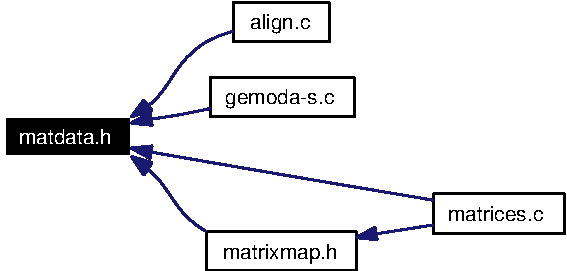
\includegraphics[width=153pt]{matdata_8h__dep__incl}
\end{center}
\end{figure}
\subsection*{Defines}
\begin{CompactItemize}
\item 
\#define \hyperlink{matdata_8h_a0}{MATRIX\_\-SIZE}~23
\end{CompactItemize}


\subsection*{Detailed Description}
This file defines the size of the scoring matrices so that we don't have to pound-include the whole \hyperlink{matrices_8h}{matrices.h} file due to worries about incompatibilities with earlier extern variable declarations.

Definition in file \hyperlink{matdata_8h-source}{matdata.h}.

\subsection*{Define Documentation}
\hypertarget{matdata_8h_a0}{
\index{matdata.h@{matdata.h}!MATRIX_SIZE@{MATRIX\_\-SIZE}}
\index{MATRIX_SIZE@{MATRIX\_\-SIZE}!matdata.h@{matdata.h}}
\subsubsection[MATRIX\_\-SIZE]{\setlength{\rightskip}{0pt plus 5cm}\#define MATRIX\_\-SIZE~23}}
\label{matdata_8h_a0}




Definition at line 10 of file matdata.h.

Referenced by main().

\hypertarget{matrices_8c}{
\section{matrices.c File Reference}
\label{matrices_8c}\index{matrices.c@{matrices.c}}
}
{\tt \#include $<$stdio.h$>$}\par
{\tt \#include $<$string.h$>$}\par
{\tt \#include \char`\"{}matdata.h\char`\"{}}\par
{\tt \#include \char`\"{}matrixmap.h\char`\"{}}\par


Include dependency graph for matrices.c:\begin{figure}[H]
\begin{center}
\leavevmode
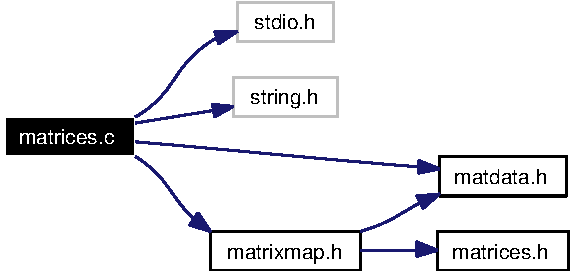
\includegraphics[width=154pt]{matrices_8c__incl}
\end{center}
\end{figure}
\subsection*{Defines}
\begin{CompactItemize}
\item 
\#define \hyperlink{matrices_8c_a0}{DEFAULT\_\-MATRIX}~\hyperlink{matrices_8h_a12}{blosum62}
\end{CompactItemize}
\subsection*{Functions}
\begin{CompactItemize}
\item 
void \hyperlink{matrices_8c_a1}{get\-Matrix\-By\-Name} (char \hyperlink{matrixmap_8h_a0}{name}\mbox{[}$\,$\mbox{]}, const int($\ast$$\ast$matp)\mbox{[}MATRIX\_\-SIZE\mbox{]})
\end{CompactItemize}


\subsection*{Detailed Description}
This file contains functions for handling scoring matrices used for the sequence based Gemoda.

Definition in file \hyperlink{matrices_8c-source}{matrices.c}.

\subsection*{Define Documentation}
\hypertarget{matrices_8c_a0}{
\index{matrices.c@{matrices.c}!DEFAULT_MATRIX@{DEFAULT\_\-MATRIX}}
\index{DEFAULT_MATRIX@{DEFAULT\_\-MATRIX}!matrices.c@{matrices.c}}
\subsubsection[DEFAULT\_\-MATRIX]{\setlength{\rightskip}{0pt plus 5cm}\#define DEFAULT\_\-MATRIX~\hyperlink{matrices_8h_a12}{blosum62}}}
\label{matrices_8c_a0}




Definition at line 7 of file matrices.c.

Referenced by get\-Matrix\-By\-Name().

\subsection*{Function Documentation}
\hypertarget{matrices_8c_a1}{
\index{matrices.c@{matrices.c}!getMatrixByName@{getMatrixByName}}
\index{getMatrixByName@{getMatrixByName}!matrices.c@{matrices.c}}
\subsubsection[getMatrixByName]{\setlength{\rightskip}{0pt plus 5cm}void get\-Matrix\-By\-Name (char {\em name}\mbox{[}$\,$\mbox{]}, const int $\ast$$\ast$ {\em matp}\mbox{[}MATRIX\_\-SIZE\mbox{]})}}
\label{matrices_8c_a1}


A simple function to take the matrix name argument given as input to gemoda and return the physical memory location of that matrix by using the matrix\_\-map construct. Input: a string containing the matrix name a pointer to a two-dimensional array. Output: None, though the value of the pointer given as input is changed to reflect the location of the matrix

Definition at line 34 of file matrices.c.

References DEFAULT\_\-MATRIX, and matrix\_\-map.

\scriptsize\begin{verbatim}35 {
36   int i;
37   for (i = 0; matrix_map[i].name != NULL; i++)
38     {
39       if (strcmp (name, matrix_map[i].name) == 0)
40     {
41       break;
42     }
43     }
44   if (matrix_map[i].name != NULL)
45     {
46       *matp = (matrix_map[i].mat);
47     }
48   else
49     {
50       *matp = (DEFAULT_MATRIX);
51     }
52 }
\end{verbatim}
\normalsize 



\hypertarget{matrices_8h}{
\section{matrices.h File Reference}
\label{matrices_8h}\index{matrices.h@{matrices.h}}
}


This graph shows which files directly or indirectly include this file:\begin{figure}[H]
\begin{center}
\leavevmode
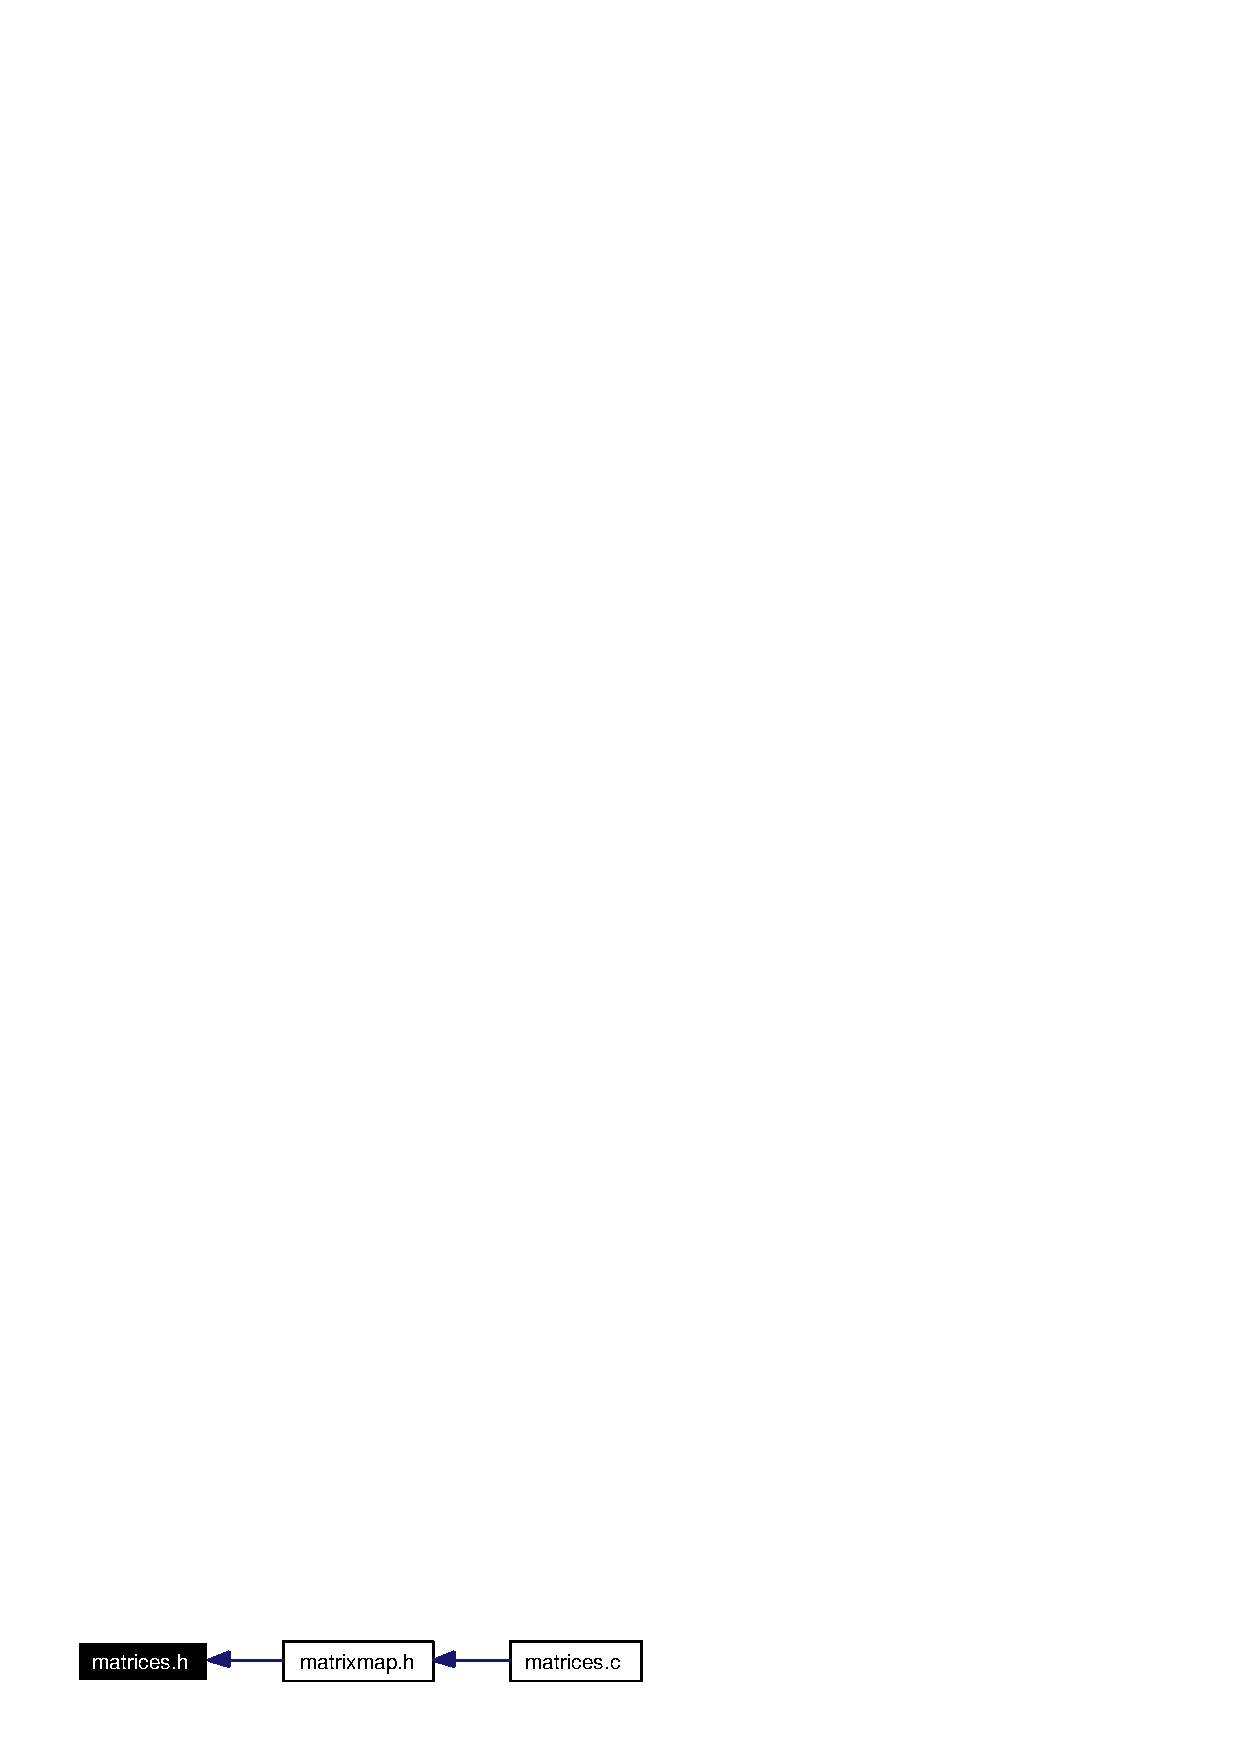
\includegraphics[width=154pt]{matrices_8h__dep__incl}
\end{center}
\end{figure}
\subsection*{Variables}
\begin{CompactItemize}
\item 
const int \hyperlink{matrices_8h_a0}{aa\-Order} \mbox{[}$\,$\mbox{]}
\item 
const int \hyperlink{matrices_8h_a1}{dna\_\-idmat} \mbox{[}MATRIX\_\-SIZE\mbox{]}\mbox{[}MATRIX\_\-SIZE\mbox{]}
\item 
const int \hyperlink{matrices_8h_a2}{identity\_\-aa} \mbox{[}MATRIX\_\-SIZE\mbox{]}\mbox{[}MATRIX\_\-SIZE\mbox{]}
\item 
const int \hyperlink{matrices_8h_a3}{idmat} \mbox{[}MATRIX\_\-SIZE\mbox{]}\mbox{[}MATRIX\_\-SIZE\mbox{]}
\item 
const int \hyperlink{matrices_8h_a4}{blosum100} \mbox{[}MATRIX\_\-SIZE\mbox{]}\mbox{[}MATRIX\_\-SIZE\mbox{]}
\item 
const int \hyperlink{matrices_8h_a5}{blosum30} \mbox{[}MATRIX\_\-SIZE\mbox{]}\mbox{[}MATRIX\_\-SIZE\mbox{]}
\item 
const int \hyperlink{matrices_8h_a6}{blosum35} \mbox{[}MATRIX\_\-SIZE\mbox{]}\mbox{[}MATRIX\_\-SIZE\mbox{]}
\item 
const int \hyperlink{matrices_8h_a7}{blosum40} \mbox{[}MATRIX\_\-SIZE\mbox{]}\mbox{[}MATRIX\_\-SIZE\mbox{]}
\item 
const int \hyperlink{matrices_8h_a8}{blosum45} \mbox{[}MATRIX\_\-SIZE\mbox{]}\mbox{[}MATRIX\_\-SIZE\mbox{]}
\item 
const int \hyperlink{matrices_8h_a9}{blosum50} \mbox{[}MATRIX\_\-SIZE\mbox{]}\mbox{[}MATRIX\_\-SIZE\mbox{]}
\item 
const int \hyperlink{matrices_8h_a10}{blosum55} \mbox{[}MATRIX\_\-SIZE\mbox{]}\mbox{[}MATRIX\_\-SIZE\mbox{]}
\item 
const int \hyperlink{matrices_8h_a11}{blosum60} \mbox{[}MATRIX\_\-SIZE\mbox{]}\mbox{[}MATRIX\_\-SIZE\mbox{]}
\item 
const int \hyperlink{matrices_8h_a12}{blosum62} \mbox{[}MATRIX\_\-SIZE\mbox{]}\mbox{[}MATRIX\_\-SIZE\mbox{]}
\item 
const int \hyperlink{matrices_8h_a13}{blosum65} \mbox{[}MATRIX\_\-SIZE\mbox{]}\mbox{[}MATRIX\_\-SIZE\mbox{]}
\item 
const int \hyperlink{matrices_8h_a14}{blosum70} \mbox{[}MATRIX\_\-SIZE\mbox{]}\mbox{[}MATRIX\_\-SIZE\mbox{]}
\item 
const int \hyperlink{matrices_8h_a15}{blosum75} \mbox{[}MATRIX\_\-SIZE\mbox{]}\mbox{[}MATRIX\_\-SIZE\mbox{]}
\item 
const int \hyperlink{matrices_8h_a16}{blosum80} \mbox{[}MATRIX\_\-SIZE\mbox{]}\mbox{[}MATRIX\_\-SIZE\mbox{]}
\item 
const int \hyperlink{matrices_8h_a17}{blosum85} \mbox{[}MATRIX\_\-SIZE\mbox{]}\mbox{[}MATRIX\_\-SIZE\mbox{]}
\item 
const int \hyperlink{matrices_8h_a18}{blosum90} \mbox{[}MATRIX\_\-SIZE\mbox{]}\mbox{[}MATRIX\_\-SIZE\mbox{]}
\item 
const int \hyperlink{matrices_8h_a19}{blosumn} \mbox{[}MATRIX\_\-SIZE\mbox{]}\mbox{[}MATRIX\_\-SIZE\mbox{]}
\item 
const int \hyperlink{matrices_8h_a20}{dayhoff} \mbox{[}MATRIX\_\-SIZE\mbox{]}\mbox{[}MATRIX\_\-SIZE\mbox{]}
\item 
const int \hyperlink{matrices_8h_a21}{pam100} \mbox{[}MATRIX\_\-SIZE\mbox{]}\mbox{[}MATRIX\_\-SIZE\mbox{]}
\item 
const int \hyperlink{matrices_8h_a22}{pam110} \mbox{[}MATRIX\_\-SIZE\mbox{]}\mbox{[}MATRIX\_\-SIZE\mbox{]}
\item 
const int \hyperlink{matrices_8h_a23}{pam120} \mbox{[}MATRIX\_\-SIZE\mbox{]}\mbox{[}MATRIX\_\-SIZE\mbox{]}
\item 
const int \hyperlink{matrices_8h_a24}{pam130} \mbox{[}MATRIX\_\-SIZE\mbox{]}\mbox{[}MATRIX\_\-SIZE\mbox{]}
\item 
const int \hyperlink{matrices_8h_a25}{pam140} \mbox{[}MATRIX\_\-SIZE\mbox{]}\mbox{[}MATRIX\_\-SIZE\mbox{]}
\item 
const int \hyperlink{matrices_8h_a26}{pam150} \mbox{[}MATRIX\_\-SIZE\mbox{]}\mbox{[}MATRIX\_\-SIZE\mbox{]}
\item 
const int \hyperlink{matrices_8h_a27}{pam160} \mbox{[}MATRIX\_\-SIZE\mbox{]}\mbox{[}MATRIX\_\-SIZE\mbox{]}
\item 
const int \hyperlink{matrices_8h_a28}{pam190} \mbox{[}MATRIX\_\-SIZE\mbox{]}\mbox{[}MATRIX\_\-SIZE\mbox{]}
\item 
const int \hyperlink{matrices_8h_a29}{pam200} \mbox{[}MATRIX\_\-SIZE\mbox{]}\mbox{[}MATRIX\_\-SIZE\mbox{]}
\item 
const int \hyperlink{matrices_8h_a30}{pam210} \mbox{[}MATRIX\_\-SIZE\mbox{]}\mbox{[}MATRIX\_\-SIZE\mbox{]}
\item 
const int \hyperlink{matrices_8h_a31}{pam220} \mbox{[}MATRIX\_\-SIZE\mbox{]}\mbox{[}MATRIX\_\-SIZE\mbox{]}
\item 
const int \hyperlink{matrices_8h_a32}{pam230} \mbox{[}MATRIX\_\-SIZE\mbox{]}\mbox{[}MATRIX\_\-SIZE\mbox{]}
\item 
const int \hyperlink{matrices_8h_a33}{pam240} \mbox{[}MATRIX\_\-SIZE\mbox{]}\mbox{[}MATRIX\_\-SIZE\mbox{]}
\item 
const int \hyperlink{matrices_8h_a34}{pam250} \mbox{[}MATRIX\_\-SIZE\mbox{]}\mbox{[}MATRIX\_\-SIZE\mbox{]}
\item 
const int \hyperlink{matrices_8h_a35}{pam260} \mbox{[}MATRIX\_\-SIZE\mbox{]}\mbox{[}MATRIX\_\-SIZE\mbox{]}
\item 
const int \hyperlink{matrices_8h_a36}{pam280} \mbox{[}MATRIX\_\-SIZE\mbox{]}\mbox{[}MATRIX\_\-SIZE\mbox{]}
\item 
const int \hyperlink{matrices_8h_a37}{pam290} \mbox{[}MATRIX\_\-SIZE\mbox{]}\mbox{[}MATRIX\_\-SIZE\mbox{]}
\item 
const int \hyperlink{matrices_8h_a38}{pam300} \mbox{[}MATRIX\_\-SIZE\mbox{]}\mbox{[}MATRIX\_\-SIZE\mbox{]}
\item 
const int \hyperlink{matrices_8h_a39}{pam310} \mbox{[}MATRIX\_\-SIZE\mbox{]}\mbox{[}MATRIX\_\-SIZE\mbox{]}
\item 
const int \hyperlink{matrices_8h_a40}{pam320} \mbox{[}MATRIX\_\-SIZE\mbox{]}\mbox{[}MATRIX\_\-SIZE\mbox{]}
\item 
const int \hyperlink{matrices_8h_a41}{pam330} \mbox{[}MATRIX\_\-SIZE\mbox{]}\mbox{[}MATRIX\_\-SIZE\mbox{]}
\item 
const int \hyperlink{matrices_8h_a42}{pam340} \mbox{[}MATRIX\_\-SIZE\mbox{]}\mbox{[}MATRIX\_\-SIZE\mbox{]}
\item 
const int \hyperlink{matrices_8h_a43}{pam360} \mbox{[}MATRIX\_\-SIZE\mbox{]}\mbox{[}MATRIX\_\-SIZE\mbox{]}
\item 
const int \hyperlink{matrices_8h_a44}{pam370} \mbox{[}MATRIX\_\-SIZE\mbox{]}\mbox{[}MATRIX\_\-SIZE\mbox{]}
\item 
const int \hyperlink{matrices_8h_a45}{pam380} \mbox{[}MATRIX\_\-SIZE\mbox{]}\mbox{[}MATRIX\_\-SIZE\mbox{]}
\item 
const int \hyperlink{matrices_8h_a46}{pam390} \mbox{[}MATRIX\_\-SIZE\mbox{]}\mbox{[}MATRIX\_\-SIZE\mbox{]}
\item 
const int \hyperlink{matrices_8h_a47}{pam400} \mbox{[}MATRIX\_\-SIZE\mbox{]}\mbox{[}MATRIX\_\-SIZE\mbox{]}
\item 
const int \hyperlink{matrices_8h_a48}{pam430} \mbox{[}MATRIX\_\-SIZE\mbox{]}\mbox{[}MATRIX\_\-SIZE\mbox{]}
\item 
const int \hyperlink{matrices_8h_a49}{pam440} \mbox{[}MATRIX\_\-SIZE\mbox{]}\mbox{[}MATRIX\_\-SIZE\mbox{]}
\item 
const int \hyperlink{matrices_8h_a50}{pam450} \mbox{[}MATRIX\_\-SIZE\mbox{]}\mbox{[}MATRIX\_\-SIZE\mbox{]}
\item 
const int \hyperlink{matrices_8h_a51}{pam460} \mbox{[}MATRIX\_\-SIZE\mbox{]}\mbox{[}MATRIX\_\-SIZE\mbox{]}
\item 
const int \hyperlink{matrices_8h_a52}{pam490} \mbox{[}MATRIX\_\-SIZE\mbox{]}\mbox{[}MATRIX\_\-SIZE\mbox{]}
\item 
const int \hyperlink{matrices_8h_a53}{pam500} \mbox{[}MATRIX\_\-SIZE\mbox{]}\mbox{[}MATRIX\_\-SIZE\mbox{]}
\item 
const int \hyperlink{matrices_8h_a54}{phat\_\-t75\_\-b73} \mbox{[}MATRIX\_\-SIZE\mbox{]}\mbox{[}MATRIX\_\-SIZE\mbox{]}
\item 
const int \hyperlink{matrices_8h_a55}{phat\_\-t80\_\-b78} \mbox{[}MATRIX\_\-SIZE\mbox{]}\mbox{[}MATRIX\_\-SIZE\mbox{]}
\item 
const int \hyperlink{matrices_8h_a56}{phat\_\-t85\_\-b82} \mbox{[}MATRIX\_\-SIZE\mbox{]}\mbox{[}MATRIX\_\-SIZE\mbox{]}
\item 
const int \hyperlink{matrices_8h_a57}{alpha\_\-mat} \mbox{[}MATRIX\_\-SIZE\mbox{]}\mbox{[}MATRIX\_\-SIZE\mbox{]}
\item 
const int \hyperlink{matrices_8h_a58}{beta\_\-mat} \mbox{[}MATRIX\_\-SIZE\mbox{]}\mbox{[}MATRIX\_\-SIZE\mbox{]}
\item 
const int \hyperlink{matrices_8h_a59}{coil\_\-mat} \mbox{[}MATRIX\_\-SIZE\mbox{]}\mbox{[}MATRIX\_\-SIZE\mbox{]}
\end{CompactItemize}


\subsection*{Detailed Description}
This file contains a number of scoring matrices, most of which are intended for comparing amino acid sequences; however a few are for DNA. In general, if a user wants to add their own matrix for use with Gemoda, they should add it to this file and recompile Gemoda.

Note that users are not restricted to 23x23 matrices. By changing aa\-Order, you can easily make matrices for comparing ANSII strings with up to 256 different characters.

All of the matrices below were obtained directly from BLAST/WU-BLAST; they are all also part of the public domain, so there is nothing intrinsic to BLAST with respect to the matrices. It was just the easiest way to get all of the matrices into our software.

The most popular matrix for amino acid sequences is blosum62.

A good location for getting new scoring matrices, such as those based on structural data, is the AAIndex. URLs tend to change, so rather than us listing it here, Google it!

Definition in file \hyperlink{matrices_8h-source}{matrices.h}.

\subsection*{Variable Documentation}
\hypertarget{matrices_8h_a0}{
\index{matrices.h@{matrices.h}!aaOrder@{aaOrder}}
\index{aaOrder@{aaOrder}!matrices.h@{matrices.h}}
\subsubsection[aaOrder]{\setlength{\rightskip}{0pt plus 5cm}const int \hyperlink{matrices_8h_a0}{aa\-Order}\mbox{[}$\,$\mbox{]}}}
\label{matrices_8h_a0}






Definition at line 32 of file matrices.h.

Referenced by align\-Mat().\hypertarget{matrices_8h_a57}{
\index{matrices.h@{matrices.h}!alpha_mat@{alpha\_\-mat}}
\index{alpha_mat@{alpha\_\-mat}!matrices.h@{matrices.h}}
\subsubsection[alpha\_\-mat]{\setlength{\rightskip}{0pt plus 5cm}const int \hyperlink{matrices_8h_a57}{alpha\_\-mat}\mbox{[}MATRIX\_\-SIZE\mbox{]}\mbox{[}MATRIX\_\-SIZE\mbox{]}}}
\label{matrices_8h_a57}






Definition at line 1398 of file matrices.h.\hypertarget{matrices_8h_a58}{
\index{matrices.h@{matrices.h}!beta_mat@{beta\_\-mat}}
\index{beta_mat@{beta\_\-mat}!matrices.h@{matrices.h}}
\subsubsection[beta\_\-mat]{\setlength{\rightskip}{0pt plus 5cm}const int \hyperlink{matrices_8h_a58}{beta\_\-mat}\mbox{[}MATRIX\_\-SIZE\mbox{]}\mbox{[}MATRIX\_\-SIZE\mbox{]}}}
\label{matrices_8h_a58}






Definition at line 1422 of file matrices.h.\hypertarget{matrices_8h_a4}{
\index{matrices.h@{matrices.h}!blosum100@{blosum100}}
\index{blosum100@{blosum100}!matrices.h@{matrices.h}}
\subsubsection[blosum100]{\setlength{\rightskip}{0pt plus 5cm}const int \hyperlink{matrices_8h_a4}{blosum100}\mbox{[}MATRIX\_\-SIZE\mbox{]}\mbox{[}MATRIX\_\-SIZE\mbox{]}}}
\label{matrices_8h_a4}






Definition at line 126 of file matrices.h.\hypertarget{matrices_8h_a5}{
\index{matrices.h@{matrices.h}!blosum30@{blosum30}}
\index{blosum30@{blosum30}!matrices.h@{matrices.h}}
\subsubsection[blosum30]{\setlength{\rightskip}{0pt plus 5cm}const int \hyperlink{matrices_8h_a5}{blosum30}\mbox{[}MATRIX\_\-SIZE\mbox{]}\mbox{[}MATRIX\_\-SIZE\mbox{]}}}
\label{matrices_8h_a5}






Definition at line 150 of file matrices.h.\hypertarget{matrices_8h_a6}{
\index{matrices.h@{matrices.h}!blosum35@{blosum35}}
\index{blosum35@{blosum35}!matrices.h@{matrices.h}}
\subsubsection[blosum35]{\setlength{\rightskip}{0pt plus 5cm}const int \hyperlink{matrices_8h_a6}{blosum35}\mbox{[}MATRIX\_\-SIZE\mbox{]}\mbox{[}MATRIX\_\-SIZE\mbox{]}}}
\label{matrices_8h_a6}






Definition at line 174 of file matrices.h.\hypertarget{matrices_8h_a7}{
\index{matrices.h@{matrices.h}!blosum40@{blosum40}}
\index{blosum40@{blosum40}!matrices.h@{matrices.h}}
\subsubsection[blosum40]{\setlength{\rightskip}{0pt plus 5cm}const int \hyperlink{matrices_8h_a7}{blosum40}\mbox{[}MATRIX\_\-SIZE\mbox{]}\mbox{[}MATRIX\_\-SIZE\mbox{]}}}
\label{matrices_8h_a7}






Definition at line 198 of file matrices.h.\hypertarget{matrices_8h_a8}{
\index{matrices.h@{matrices.h}!blosum45@{blosum45}}
\index{blosum45@{blosum45}!matrices.h@{matrices.h}}
\subsubsection[blosum45]{\setlength{\rightskip}{0pt plus 5cm}const int \hyperlink{matrices_8h_a8}{blosum45}\mbox{[}MATRIX\_\-SIZE\mbox{]}\mbox{[}MATRIX\_\-SIZE\mbox{]}}}
\label{matrices_8h_a8}






Definition at line 222 of file matrices.h.\hypertarget{matrices_8h_a9}{
\index{matrices.h@{matrices.h}!blosum50@{blosum50}}
\index{blosum50@{blosum50}!matrices.h@{matrices.h}}
\subsubsection[blosum50]{\setlength{\rightskip}{0pt plus 5cm}const int \hyperlink{matrices_8h_a9}{blosum50}\mbox{[}MATRIX\_\-SIZE\mbox{]}\mbox{[}MATRIX\_\-SIZE\mbox{]}}}
\label{matrices_8h_a9}






Definition at line 246 of file matrices.h.\hypertarget{matrices_8h_a10}{
\index{matrices.h@{matrices.h}!blosum55@{blosum55}}
\index{blosum55@{blosum55}!matrices.h@{matrices.h}}
\subsubsection[blosum55]{\setlength{\rightskip}{0pt plus 5cm}const int \hyperlink{matrices_8h_a10}{blosum55}\mbox{[}MATRIX\_\-SIZE\mbox{]}\mbox{[}MATRIX\_\-SIZE\mbox{]}}}
\label{matrices_8h_a10}






Definition at line 270 of file matrices.h.\hypertarget{matrices_8h_a11}{
\index{matrices.h@{matrices.h}!blosum60@{blosum60}}
\index{blosum60@{blosum60}!matrices.h@{matrices.h}}
\subsubsection[blosum60]{\setlength{\rightskip}{0pt plus 5cm}const int \hyperlink{matrices_8h_a11}{blosum60}\mbox{[}MATRIX\_\-SIZE\mbox{]}\mbox{[}MATRIX\_\-SIZE\mbox{]}}}
\label{matrices_8h_a11}






Definition at line 294 of file matrices.h.\hypertarget{matrices_8h_a12}{
\index{matrices.h@{matrices.h}!blosum62@{blosum62}}
\index{blosum62@{blosum62}!matrices.h@{matrices.h}}
\subsubsection[blosum62]{\setlength{\rightskip}{0pt plus 5cm}const int \hyperlink{matrices_8h_a12}{blosum62}\mbox{[}MATRIX\_\-SIZE\mbox{]}\mbox{[}MATRIX\_\-SIZE\mbox{]}}}
\label{matrices_8h_a12}






Definition at line 318 of file matrices.h.\hypertarget{matrices_8h_a13}{
\index{matrices.h@{matrices.h}!blosum65@{blosum65}}
\index{blosum65@{blosum65}!matrices.h@{matrices.h}}
\subsubsection[blosum65]{\setlength{\rightskip}{0pt plus 5cm}const int \hyperlink{matrices_8h_a13}{blosum65}\mbox{[}MATRIX\_\-SIZE\mbox{]}\mbox{[}MATRIX\_\-SIZE\mbox{]}}}
\label{matrices_8h_a13}






Definition at line 342 of file matrices.h.\hypertarget{matrices_8h_a14}{
\index{matrices.h@{matrices.h}!blosum70@{blosum70}}
\index{blosum70@{blosum70}!matrices.h@{matrices.h}}
\subsubsection[blosum70]{\setlength{\rightskip}{0pt plus 5cm}const int \hyperlink{matrices_8h_a14}{blosum70}\mbox{[}MATRIX\_\-SIZE\mbox{]}\mbox{[}MATRIX\_\-SIZE\mbox{]}}}
\label{matrices_8h_a14}






Definition at line 366 of file matrices.h.\hypertarget{matrices_8h_a15}{
\index{matrices.h@{matrices.h}!blosum75@{blosum75}}
\index{blosum75@{blosum75}!matrices.h@{matrices.h}}
\subsubsection[blosum75]{\setlength{\rightskip}{0pt plus 5cm}const int \hyperlink{matrices_8h_a15}{blosum75}\mbox{[}MATRIX\_\-SIZE\mbox{]}\mbox{[}MATRIX\_\-SIZE\mbox{]}}}
\label{matrices_8h_a15}






Definition at line 390 of file matrices.h.\hypertarget{matrices_8h_a16}{
\index{matrices.h@{matrices.h}!blosum80@{blosum80}}
\index{blosum80@{blosum80}!matrices.h@{matrices.h}}
\subsubsection[blosum80]{\setlength{\rightskip}{0pt plus 5cm}const int \hyperlink{matrices_8h_a16}{blosum80}\mbox{[}MATRIX\_\-SIZE\mbox{]}\mbox{[}MATRIX\_\-SIZE\mbox{]}}}
\label{matrices_8h_a16}






Definition at line 414 of file matrices.h.\hypertarget{matrices_8h_a17}{
\index{matrices.h@{matrices.h}!blosum85@{blosum85}}
\index{blosum85@{blosum85}!matrices.h@{matrices.h}}
\subsubsection[blosum85]{\setlength{\rightskip}{0pt plus 5cm}const int \hyperlink{matrices_8h_a17}{blosum85}\mbox{[}MATRIX\_\-SIZE\mbox{]}\mbox{[}MATRIX\_\-SIZE\mbox{]}}}
\label{matrices_8h_a17}






Definition at line 438 of file matrices.h.\hypertarget{matrices_8h_a18}{
\index{matrices.h@{matrices.h}!blosum90@{blosum90}}
\index{blosum90@{blosum90}!matrices.h@{matrices.h}}
\subsubsection[blosum90]{\setlength{\rightskip}{0pt plus 5cm}const int \hyperlink{matrices_8h_a18}{blosum90}\mbox{[}MATRIX\_\-SIZE\mbox{]}\mbox{[}MATRIX\_\-SIZE\mbox{]}}}
\label{matrices_8h_a18}






Definition at line 462 of file matrices.h.\hypertarget{matrices_8h_a19}{
\index{matrices.h@{matrices.h}!blosumn@{blosumn}}
\index{blosumn@{blosumn}!matrices.h@{matrices.h}}
\subsubsection[blosumn]{\setlength{\rightskip}{0pt plus 5cm}const int \hyperlink{matrices_8h_a19}{blosumn}\mbox{[}MATRIX\_\-SIZE\mbox{]}\mbox{[}MATRIX\_\-SIZE\mbox{]}}}
\label{matrices_8h_a19}






Definition at line 486 of file matrices.h.\hypertarget{matrices_8h_a59}{
\index{matrices.h@{matrices.h}!coil_mat@{coil\_\-mat}}
\index{coil_mat@{coil\_\-mat}!matrices.h@{matrices.h}}
\subsubsection[coil\_\-mat]{\setlength{\rightskip}{0pt plus 5cm}const int \hyperlink{matrices_8h_a59}{coil\_\-mat}\mbox{[}MATRIX\_\-SIZE\mbox{]}\mbox{[}MATRIX\_\-SIZE\mbox{]}}}
\label{matrices_8h_a59}






Definition at line 1446 of file matrices.h.\hypertarget{matrices_8h_a20}{
\index{matrices.h@{matrices.h}!dayhoff@{dayhoff}}
\index{dayhoff@{dayhoff}!matrices.h@{matrices.h}}
\subsubsection[dayhoff]{\setlength{\rightskip}{0pt plus 5cm}const int \hyperlink{matrices_8h_a20}{dayhoff}\mbox{[}MATRIX\_\-SIZE\mbox{]}\mbox{[}MATRIX\_\-SIZE\mbox{]}}}
\label{matrices_8h_a20}






Definition at line 510 of file matrices.h.\hypertarget{matrices_8h_a1}{
\index{matrices.h@{matrices.h}!dna_idmat@{dna\_\-idmat}}
\index{dna_idmat@{dna\_\-idmat}!matrices.h@{matrices.h}}
\subsubsection[dna\_\-idmat]{\setlength{\rightskip}{0pt plus 5cm}const int \hyperlink{matrices_8h_a1}{dna\_\-idmat}\mbox{[}MATRIX\_\-SIZE\mbox{]}\mbox{[}MATRIX\_\-SIZE\mbox{]}}}
\label{matrices_8h_a1}






Definition at line 50 of file matrices.h.\hypertarget{matrices_8h_a2}{
\index{matrices.h@{matrices.h}!identity_aa@{identity\_\-aa}}
\index{identity_aa@{identity\_\-aa}!matrices.h@{matrices.h}}
\subsubsection[identity\_\-aa]{\setlength{\rightskip}{0pt plus 5cm}const int \hyperlink{matrices_8h_a2}{identity\_\-aa}\mbox{[}MATRIX\_\-SIZE\mbox{]}\mbox{[}MATRIX\_\-SIZE\mbox{]}}}
\label{matrices_8h_a2}






Definition at line 76 of file matrices.h.\hypertarget{matrices_8h_a3}{
\index{matrices.h@{matrices.h}!idmat@{idmat}}
\index{idmat@{idmat}!matrices.h@{matrices.h}}
\subsubsection[idmat]{\setlength{\rightskip}{0pt plus 5cm}const int \hyperlink{matrices_8h_a3}{idmat}\mbox{[}MATRIX\_\-SIZE\mbox{]}\mbox{[}MATRIX\_\-SIZE\mbox{]}}}
\label{matrices_8h_a3}






Definition at line 101 of file matrices.h.\hypertarget{matrices_8h_a21}{
\index{matrices.h@{matrices.h}!pam100@{pam100}}
\index{pam100@{pam100}!matrices.h@{matrices.h}}
\subsubsection[pam100]{\setlength{\rightskip}{0pt plus 5cm}const int \hyperlink{matrices_8h_a21}{pam100}\mbox{[}MATRIX\_\-SIZE\mbox{]}\mbox{[}MATRIX\_\-SIZE\mbox{]}}}
\label{matrices_8h_a21}






Definition at line 534 of file matrices.h.\hypertarget{matrices_8h_a22}{
\index{matrices.h@{matrices.h}!pam110@{pam110}}
\index{pam110@{pam110}!matrices.h@{matrices.h}}
\subsubsection[pam110]{\setlength{\rightskip}{0pt plus 5cm}const int \hyperlink{matrices_8h_a22}{pam110}\mbox{[}MATRIX\_\-SIZE\mbox{]}\mbox{[}MATRIX\_\-SIZE\mbox{]}}}
\label{matrices_8h_a22}






Definition at line 558 of file matrices.h.\hypertarget{matrices_8h_a23}{
\index{matrices.h@{matrices.h}!pam120@{pam120}}
\index{pam120@{pam120}!matrices.h@{matrices.h}}
\subsubsection[pam120]{\setlength{\rightskip}{0pt plus 5cm}const int \hyperlink{matrices_8h_a23}{pam120}\mbox{[}MATRIX\_\-SIZE\mbox{]}\mbox{[}MATRIX\_\-SIZE\mbox{]}}}
\label{matrices_8h_a23}






Definition at line 582 of file matrices.h.\hypertarget{matrices_8h_a24}{
\index{matrices.h@{matrices.h}!pam130@{pam130}}
\index{pam130@{pam130}!matrices.h@{matrices.h}}
\subsubsection[pam130]{\setlength{\rightskip}{0pt plus 5cm}const int \hyperlink{matrices_8h_a24}{pam130}\mbox{[}MATRIX\_\-SIZE\mbox{]}\mbox{[}MATRIX\_\-SIZE\mbox{]}}}
\label{matrices_8h_a24}






Definition at line 606 of file matrices.h.\hypertarget{matrices_8h_a25}{
\index{matrices.h@{matrices.h}!pam140@{pam140}}
\index{pam140@{pam140}!matrices.h@{matrices.h}}
\subsubsection[pam140]{\setlength{\rightskip}{0pt plus 5cm}const int \hyperlink{matrices_8h_a25}{pam140}\mbox{[}MATRIX\_\-SIZE\mbox{]}\mbox{[}MATRIX\_\-SIZE\mbox{]}}}
\label{matrices_8h_a25}






Definition at line 630 of file matrices.h.\hypertarget{matrices_8h_a26}{
\index{matrices.h@{matrices.h}!pam150@{pam150}}
\index{pam150@{pam150}!matrices.h@{matrices.h}}
\subsubsection[pam150]{\setlength{\rightskip}{0pt plus 5cm}const int \hyperlink{matrices_8h_a26}{pam150}\mbox{[}MATRIX\_\-SIZE\mbox{]}\mbox{[}MATRIX\_\-SIZE\mbox{]}}}
\label{matrices_8h_a26}






Definition at line 654 of file matrices.h.\hypertarget{matrices_8h_a27}{
\index{matrices.h@{matrices.h}!pam160@{pam160}}
\index{pam160@{pam160}!matrices.h@{matrices.h}}
\subsubsection[pam160]{\setlength{\rightskip}{0pt plus 5cm}const int \hyperlink{matrices_8h_a27}{pam160}\mbox{[}MATRIX\_\-SIZE\mbox{]}\mbox{[}MATRIX\_\-SIZE\mbox{]}}}
\label{matrices_8h_a27}






Definition at line 678 of file matrices.h.\hypertarget{matrices_8h_a28}{
\index{matrices.h@{matrices.h}!pam190@{pam190}}
\index{pam190@{pam190}!matrices.h@{matrices.h}}
\subsubsection[pam190]{\setlength{\rightskip}{0pt plus 5cm}const int \hyperlink{matrices_8h_a28}{pam190}\mbox{[}MATRIX\_\-SIZE\mbox{]}\mbox{[}MATRIX\_\-SIZE\mbox{]}}}
\label{matrices_8h_a28}






Definition at line 702 of file matrices.h.\hypertarget{matrices_8h_a29}{
\index{matrices.h@{matrices.h}!pam200@{pam200}}
\index{pam200@{pam200}!matrices.h@{matrices.h}}
\subsubsection[pam200]{\setlength{\rightskip}{0pt plus 5cm}const int \hyperlink{matrices_8h_a29}{pam200}\mbox{[}MATRIX\_\-SIZE\mbox{]}\mbox{[}MATRIX\_\-SIZE\mbox{]}}}
\label{matrices_8h_a29}






Definition at line 726 of file matrices.h.\hypertarget{matrices_8h_a30}{
\index{matrices.h@{matrices.h}!pam210@{pam210}}
\index{pam210@{pam210}!matrices.h@{matrices.h}}
\subsubsection[pam210]{\setlength{\rightskip}{0pt plus 5cm}const int \hyperlink{matrices_8h_a30}{pam210}\mbox{[}MATRIX\_\-SIZE\mbox{]}\mbox{[}MATRIX\_\-SIZE\mbox{]}}}
\label{matrices_8h_a30}






Definition at line 750 of file matrices.h.\hypertarget{matrices_8h_a31}{
\index{matrices.h@{matrices.h}!pam220@{pam220}}
\index{pam220@{pam220}!matrices.h@{matrices.h}}
\subsubsection[pam220]{\setlength{\rightskip}{0pt plus 5cm}const int \hyperlink{matrices_8h_a31}{pam220}\mbox{[}MATRIX\_\-SIZE\mbox{]}\mbox{[}MATRIX\_\-SIZE\mbox{]}}}
\label{matrices_8h_a31}






Definition at line 774 of file matrices.h.\hypertarget{matrices_8h_a32}{
\index{matrices.h@{matrices.h}!pam230@{pam230}}
\index{pam230@{pam230}!matrices.h@{matrices.h}}
\subsubsection[pam230]{\setlength{\rightskip}{0pt plus 5cm}const int \hyperlink{matrices_8h_a32}{pam230}\mbox{[}MATRIX\_\-SIZE\mbox{]}\mbox{[}MATRIX\_\-SIZE\mbox{]}}}
\label{matrices_8h_a32}






Definition at line 798 of file matrices.h.\hypertarget{matrices_8h_a33}{
\index{matrices.h@{matrices.h}!pam240@{pam240}}
\index{pam240@{pam240}!matrices.h@{matrices.h}}
\subsubsection[pam240]{\setlength{\rightskip}{0pt plus 5cm}const int \hyperlink{matrices_8h_a33}{pam240}\mbox{[}MATRIX\_\-SIZE\mbox{]}\mbox{[}MATRIX\_\-SIZE\mbox{]}}}
\label{matrices_8h_a33}






Definition at line 822 of file matrices.h.\hypertarget{matrices_8h_a34}{
\index{matrices.h@{matrices.h}!pam250@{pam250}}
\index{pam250@{pam250}!matrices.h@{matrices.h}}
\subsubsection[pam250]{\setlength{\rightskip}{0pt plus 5cm}const int \hyperlink{matrices_8h_a34}{pam250}\mbox{[}MATRIX\_\-SIZE\mbox{]}\mbox{[}MATRIX\_\-SIZE\mbox{]}}}
\label{matrices_8h_a34}






Definition at line 846 of file matrices.h.\hypertarget{matrices_8h_a35}{
\index{matrices.h@{matrices.h}!pam260@{pam260}}
\index{pam260@{pam260}!matrices.h@{matrices.h}}
\subsubsection[pam260]{\setlength{\rightskip}{0pt plus 5cm}const int \hyperlink{matrices_8h_a35}{pam260}\mbox{[}MATRIX\_\-SIZE\mbox{]}\mbox{[}MATRIX\_\-SIZE\mbox{]}}}
\label{matrices_8h_a35}






Definition at line 870 of file matrices.h.\hypertarget{matrices_8h_a36}{
\index{matrices.h@{matrices.h}!pam280@{pam280}}
\index{pam280@{pam280}!matrices.h@{matrices.h}}
\subsubsection[pam280]{\setlength{\rightskip}{0pt plus 5cm}const int \hyperlink{matrices_8h_a36}{pam280}\mbox{[}MATRIX\_\-SIZE\mbox{]}\mbox{[}MATRIX\_\-SIZE\mbox{]}}}
\label{matrices_8h_a36}






Definition at line 894 of file matrices.h.\hypertarget{matrices_8h_a37}{
\index{matrices.h@{matrices.h}!pam290@{pam290}}
\index{pam290@{pam290}!matrices.h@{matrices.h}}
\subsubsection[pam290]{\setlength{\rightskip}{0pt plus 5cm}const int \hyperlink{matrices_8h_a37}{pam290}\mbox{[}MATRIX\_\-SIZE\mbox{]}\mbox{[}MATRIX\_\-SIZE\mbox{]}}}
\label{matrices_8h_a37}






Definition at line 918 of file matrices.h.\hypertarget{matrices_8h_a38}{
\index{matrices.h@{matrices.h}!pam300@{pam300}}
\index{pam300@{pam300}!matrices.h@{matrices.h}}
\subsubsection[pam300]{\setlength{\rightskip}{0pt plus 5cm}const int \hyperlink{matrices_8h_a38}{pam300}\mbox{[}MATRIX\_\-SIZE\mbox{]}\mbox{[}MATRIX\_\-SIZE\mbox{]}}}
\label{matrices_8h_a38}






Definition at line 942 of file matrices.h.\hypertarget{matrices_8h_a39}{
\index{matrices.h@{matrices.h}!pam310@{pam310}}
\index{pam310@{pam310}!matrices.h@{matrices.h}}
\subsubsection[pam310]{\setlength{\rightskip}{0pt plus 5cm}const int \hyperlink{matrices_8h_a39}{pam310}\mbox{[}MATRIX\_\-SIZE\mbox{]}\mbox{[}MATRIX\_\-SIZE\mbox{]}}}
\label{matrices_8h_a39}






Definition at line 966 of file matrices.h.\hypertarget{matrices_8h_a40}{
\index{matrices.h@{matrices.h}!pam320@{pam320}}
\index{pam320@{pam320}!matrices.h@{matrices.h}}
\subsubsection[pam320]{\setlength{\rightskip}{0pt plus 5cm}const int \hyperlink{matrices_8h_a40}{pam320}\mbox{[}MATRIX\_\-SIZE\mbox{]}\mbox{[}MATRIX\_\-SIZE\mbox{]}}}
\label{matrices_8h_a40}






Definition at line 990 of file matrices.h.\hypertarget{matrices_8h_a41}{
\index{matrices.h@{matrices.h}!pam330@{pam330}}
\index{pam330@{pam330}!matrices.h@{matrices.h}}
\subsubsection[pam330]{\setlength{\rightskip}{0pt plus 5cm}const int \hyperlink{matrices_8h_a41}{pam330}\mbox{[}MATRIX\_\-SIZE\mbox{]}\mbox{[}MATRIX\_\-SIZE\mbox{]}}}
\label{matrices_8h_a41}






Definition at line 1014 of file matrices.h.\hypertarget{matrices_8h_a42}{
\index{matrices.h@{matrices.h}!pam340@{pam340}}
\index{pam340@{pam340}!matrices.h@{matrices.h}}
\subsubsection[pam340]{\setlength{\rightskip}{0pt plus 5cm}const int \hyperlink{matrices_8h_a42}{pam340}\mbox{[}MATRIX\_\-SIZE\mbox{]}\mbox{[}MATRIX\_\-SIZE\mbox{]}}}
\label{matrices_8h_a42}






Definition at line 1038 of file matrices.h.\hypertarget{matrices_8h_a43}{
\index{matrices.h@{matrices.h}!pam360@{pam360}}
\index{pam360@{pam360}!matrices.h@{matrices.h}}
\subsubsection[pam360]{\setlength{\rightskip}{0pt plus 5cm}const int \hyperlink{matrices_8h_a43}{pam360}\mbox{[}MATRIX\_\-SIZE\mbox{]}\mbox{[}MATRIX\_\-SIZE\mbox{]}}}
\label{matrices_8h_a43}






Definition at line 1062 of file matrices.h.\hypertarget{matrices_8h_a44}{
\index{matrices.h@{matrices.h}!pam370@{pam370}}
\index{pam370@{pam370}!matrices.h@{matrices.h}}
\subsubsection[pam370]{\setlength{\rightskip}{0pt plus 5cm}const int \hyperlink{matrices_8h_a44}{pam370}\mbox{[}MATRIX\_\-SIZE\mbox{]}\mbox{[}MATRIX\_\-SIZE\mbox{]}}}
\label{matrices_8h_a44}






Definition at line 1086 of file matrices.h.\hypertarget{matrices_8h_a45}{
\index{matrices.h@{matrices.h}!pam380@{pam380}}
\index{pam380@{pam380}!matrices.h@{matrices.h}}
\subsubsection[pam380]{\setlength{\rightskip}{0pt plus 5cm}const int \hyperlink{matrices_8h_a45}{pam380}\mbox{[}MATRIX\_\-SIZE\mbox{]}\mbox{[}MATRIX\_\-SIZE\mbox{]}}}
\label{matrices_8h_a45}






Definition at line 1110 of file matrices.h.\hypertarget{matrices_8h_a46}{
\index{matrices.h@{matrices.h}!pam390@{pam390}}
\index{pam390@{pam390}!matrices.h@{matrices.h}}
\subsubsection[pam390]{\setlength{\rightskip}{0pt plus 5cm}const int \hyperlink{matrices_8h_a46}{pam390}\mbox{[}MATRIX\_\-SIZE\mbox{]}\mbox{[}MATRIX\_\-SIZE\mbox{]}}}
\label{matrices_8h_a46}






Definition at line 1134 of file matrices.h.\hypertarget{matrices_8h_a47}{
\index{matrices.h@{matrices.h}!pam400@{pam400}}
\index{pam400@{pam400}!matrices.h@{matrices.h}}
\subsubsection[pam400]{\setlength{\rightskip}{0pt plus 5cm}const int \hyperlink{matrices_8h_a47}{pam400}\mbox{[}MATRIX\_\-SIZE\mbox{]}\mbox{[}MATRIX\_\-SIZE\mbox{]}}}
\label{matrices_8h_a47}






Definition at line 1158 of file matrices.h.\hypertarget{matrices_8h_a48}{
\index{matrices.h@{matrices.h}!pam430@{pam430}}
\index{pam430@{pam430}!matrices.h@{matrices.h}}
\subsubsection[pam430]{\setlength{\rightskip}{0pt plus 5cm}const int \hyperlink{matrices_8h_a48}{pam430}\mbox{[}MATRIX\_\-SIZE\mbox{]}\mbox{[}MATRIX\_\-SIZE\mbox{]}}}
\label{matrices_8h_a48}






Definition at line 1182 of file matrices.h.\hypertarget{matrices_8h_a49}{
\index{matrices.h@{matrices.h}!pam440@{pam440}}
\index{pam440@{pam440}!matrices.h@{matrices.h}}
\subsubsection[pam440]{\setlength{\rightskip}{0pt plus 5cm}const int \hyperlink{matrices_8h_a49}{pam440}\mbox{[}MATRIX\_\-SIZE\mbox{]}\mbox{[}MATRIX\_\-SIZE\mbox{]}}}
\label{matrices_8h_a49}






Definition at line 1206 of file matrices.h.\hypertarget{matrices_8h_a50}{
\index{matrices.h@{matrices.h}!pam450@{pam450}}
\index{pam450@{pam450}!matrices.h@{matrices.h}}
\subsubsection[pam450]{\setlength{\rightskip}{0pt plus 5cm}const int \hyperlink{matrices_8h_a50}{pam450}\mbox{[}MATRIX\_\-SIZE\mbox{]}\mbox{[}MATRIX\_\-SIZE\mbox{]}}}
\label{matrices_8h_a50}






Definition at line 1230 of file matrices.h.\hypertarget{matrices_8h_a51}{
\index{matrices.h@{matrices.h}!pam460@{pam460}}
\index{pam460@{pam460}!matrices.h@{matrices.h}}
\subsubsection[pam460]{\setlength{\rightskip}{0pt plus 5cm}const int \hyperlink{matrices_8h_a51}{pam460}\mbox{[}MATRIX\_\-SIZE\mbox{]}\mbox{[}MATRIX\_\-SIZE\mbox{]}}}
\label{matrices_8h_a51}






Definition at line 1254 of file matrices.h.\hypertarget{matrices_8h_a52}{
\index{matrices.h@{matrices.h}!pam490@{pam490}}
\index{pam490@{pam490}!matrices.h@{matrices.h}}
\subsubsection[pam490]{\setlength{\rightskip}{0pt plus 5cm}const int \hyperlink{matrices_8h_a52}{pam490}\mbox{[}MATRIX\_\-SIZE\mbox{]}\mbox{[}MATRIX\_\-SIZE\mbox{]}}}
\label{matrices_8h_a52}






Definition at line 1278 of file matrices.h.\hypertarget{matrices_8h_a53}{
\index{matrices.h@{matrices.h}!pam500@{pam500}}
\index{pam500@{pam500}!matrices.h@{matrices.h}}
\subsubsection[pam500]{\setlength{\rightskip}{0pt plus 5cm}const int \hyperlink{matrices_8h_a53}{pam500}\mbox{[}MATRIX\_\-SIZE\mbox{]}\mbox{[}MATRIX\_\-SIZE\mbox{]}}}
\label{matrices_8h_a53}






Definition at line 1302 of file matrices.h.\hypertarget{matrices_8h_a54}{
\index{matrices.h@{matrices.h}!phat_t75_b73@{phat\_\-t75\_\-b73}}
\index{phat_t75_b73@{phat\_\-t75\_\-b73}!matrices.h@{matrices.h}}
\subsubsection[phat\_\-t75\_\-b73]{\setlength{\rightskip}{0pt plus 5cm}const int \hyperlink{matrices_8h_a54}{phat\_\-t75\_\-b73}\mbox{[}MATRIX\_\-SIZE\mbox{]}\mbox{[}MATRIX\_\-SIZE\mbox{]}}}
\label{matrices_8h_a54}






Definition at line 1326 of file matrices.h.\hypertarget{matrices_8h_a55}{
\index{matrices.h@{matrices.h}!phat_t80_b78@{phat\_\-t80\_\-b78}}
\index{phat_t80_b78@{phat\_\-t80\_\-b78}!matrices.h@{matrices.h}}
\subsubsection[phat\_\-t80\_\-b78]{\setlength{\rightskip}{0pt plus 5cm}const int \hyperlink{matrices_8h_a55}{phat\_\-t80\_\-b78}\mbox{[}MATRIX\_\-SIZE\mbox{]}\mbox{[}MATRIX\_\-SIZE\mbox{]}}}
\label{matrices_8h_a55}






Definition at line 1350 of file matrices.h.\hypertarget{matrices_8h_a56}{
\index{matrices.h@{matrices.h}!phat_t85_b82@{phat\_\-t85\_\-b82}}
\index{phat_t85_b82@{phat\_\-t85\_\-b82}!matrices.h@{matrices.h}}
\subsubsection[phat\_\-t85\_\-b82]{\setlength{\rightskip}{0pt plus 5cm}const int \hyperlink{matrices_8h_a56}{phat\_\-t85\_\-b82}\mbox{[}MATRIX\_\-SIZE\mbox{]}\mbox{[}MATRIX\_\-SIZE\mbox{]}}}
\label{matrices_8h_a56}






Definition at line 1374 of file matrices.h.

\hypertarget{matrixmap_8h}{
\section{matrixmap.h File Reference}
\label{matrixmap_8h}\index{matrixmap.h@{matrixmap.h}}
}
{\tt \#include \char`\"{}matdata.h\char`\"{}}\par
{\tt \#include \char`\"{}matrices.h\char`\"{}}\par


Include dependency graph for matrixmap.h:\begin{figure}[H]
\begin{center}
\leavevmode
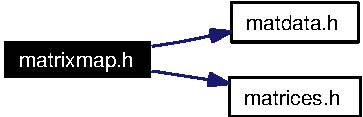
\includegraphics[width=104pt]{matrixmap_8h__incl}
\end{center}
\end{figure}


This graph shows which files directly or indirectly include this file:\begin{figure}[H]
\begin{center}
\leavevmode
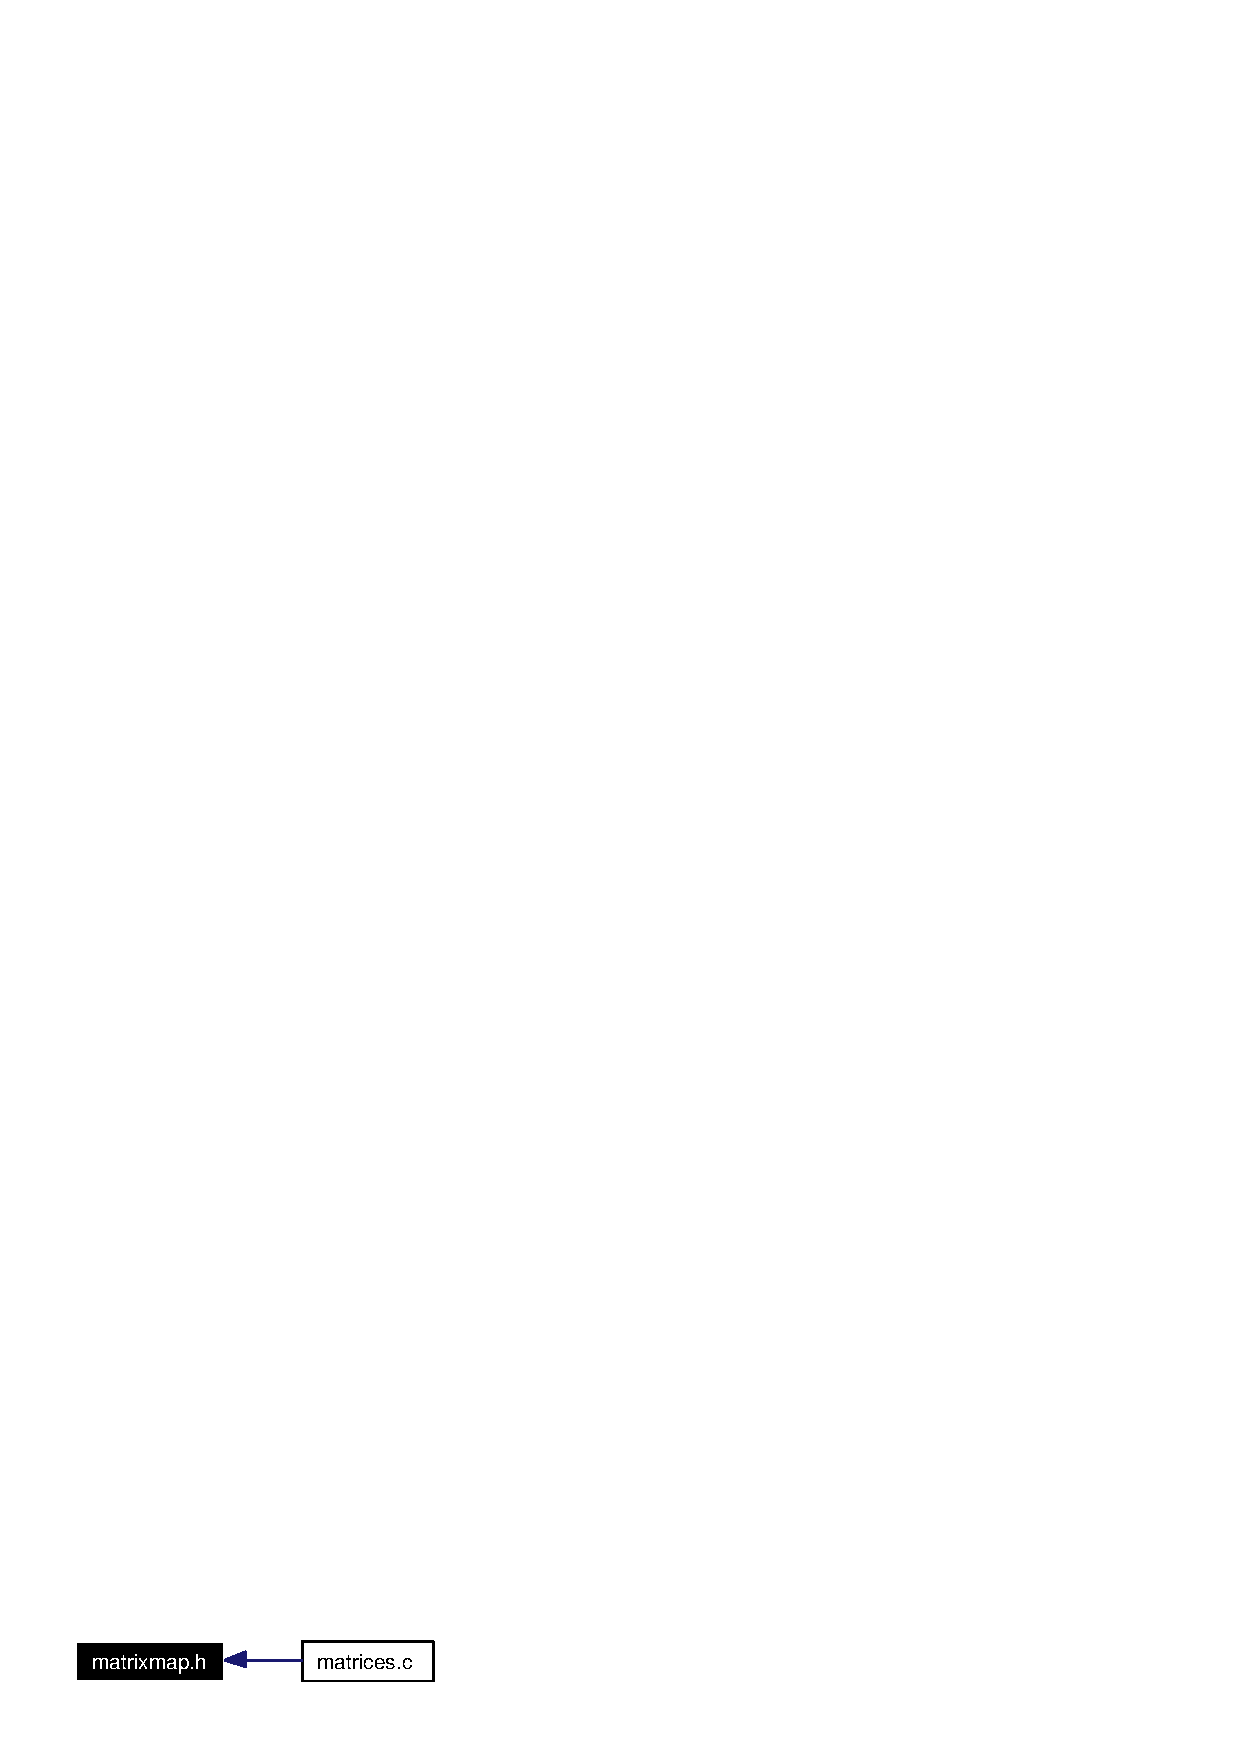
\includegraphics[width=104pt]{matrixmap_8h__dep__incl}
\end{center}
\end{figure}
\subsection*{Variables}
\begin{CompactItemize}
\item 
\begin{tabbing}
xx\=xx\=xx\=xx\=xx\=xx\=xx\=xx\=xx\=\kill
struct \{\\
\>char $\ast$ \hyperlink{matrixmap_8h_a0}{name}\\
\>const int($\ast$ \hyperlink{matrixmap_8h_a1}{mat} )\mbox{[}MATRIX\_SIZE\mbox{]}\\
\} \hyperlink{matrixmap_8h_a2}{matrix\_map} \mbox{[}$\,$\mbox{]}\\

\end{tabbing}\end{CompactItemize}


\subsection*{Detailed Description}
This file contains structures and functions for handling scoring matrices.

Definition in file \hyperlink{matrixmap_8h-source}{matrixmap.h}.

\subsection*{Variable Documentation}
\hypertarget{matrixmap_8h_a1}{
\index{matrixmap.h@{matrixmap.h}!mat@{mat}}
\index{mat@{mat}!matrixmap.h@{matrixmap.h}}
\subsubsection[mat]{\setlength{\rightskip}{0pt plus 5cm}const int($\ast$ \hyperlink{matrixmap_8h_a1}{mat})\mbox{[}MATRIX\_\-SIZE\mbox{]}}}
\label{matrixmap_8h_a1}




Definition at line 15 of file matrixmap.h.

Referenced by align\-Mat(), align\-Words\-Mat\_\-bit(), and main().\hypertarget{matrixmap_8h_a2}{
\index{matrixmap.h@{matrixmap.h}!matrix_map@{matrix\_\-map}}
\index{matrix_map@{matrix\_\-map}!matrixmap.h@{matrixmap.h}}
\subsubsection[matrix\_\-map]{\setlength{\rightskip}{0pt plus 5cm}struct \{ ... \}   \hyperlink{matrixmap_8h_a2}{matrix\_\-map}\mbox{[}$\,$\mbox{]}}}
\label{matrixmap_8h_a2}


This data structure maps the names of common matrices to the names of their variables

Referenced by get\-Matrix\-By\-Name().\hypertarget{matrixmap_8h_a0}{
\index{matrixmap.h@{matrixmap.h}!name@{name}}
\index{name@{name}!matrixmap.h@{matrixmap.h}}
\subsubsection[name]{\setlength{\rightskip}{0pt plus 5cm}char$\ast$ \hyperlink{matrixmap_8h_a0}{name}}}
\label{matrixmap_8h_a0}




Definition at line 14 of file matrixmap.h.

\hypertarget{newConv_8c}{
\section{new\-Conv.c File Reference}
\label{newConv_8c}\index{newConv.c@{newConv.c}}
}
{\tt \#include \char`\"{}bit\-Set.h\char`\"{}}\par
{\tt \#include $<$errno.h$>$}\par
{\tt \#include \char`\"{}convll.h\char`\"{}}\par


Include dependency graph for new\-Conv.c:\begin{figure}[H]
\begin{center}
\leavevmode
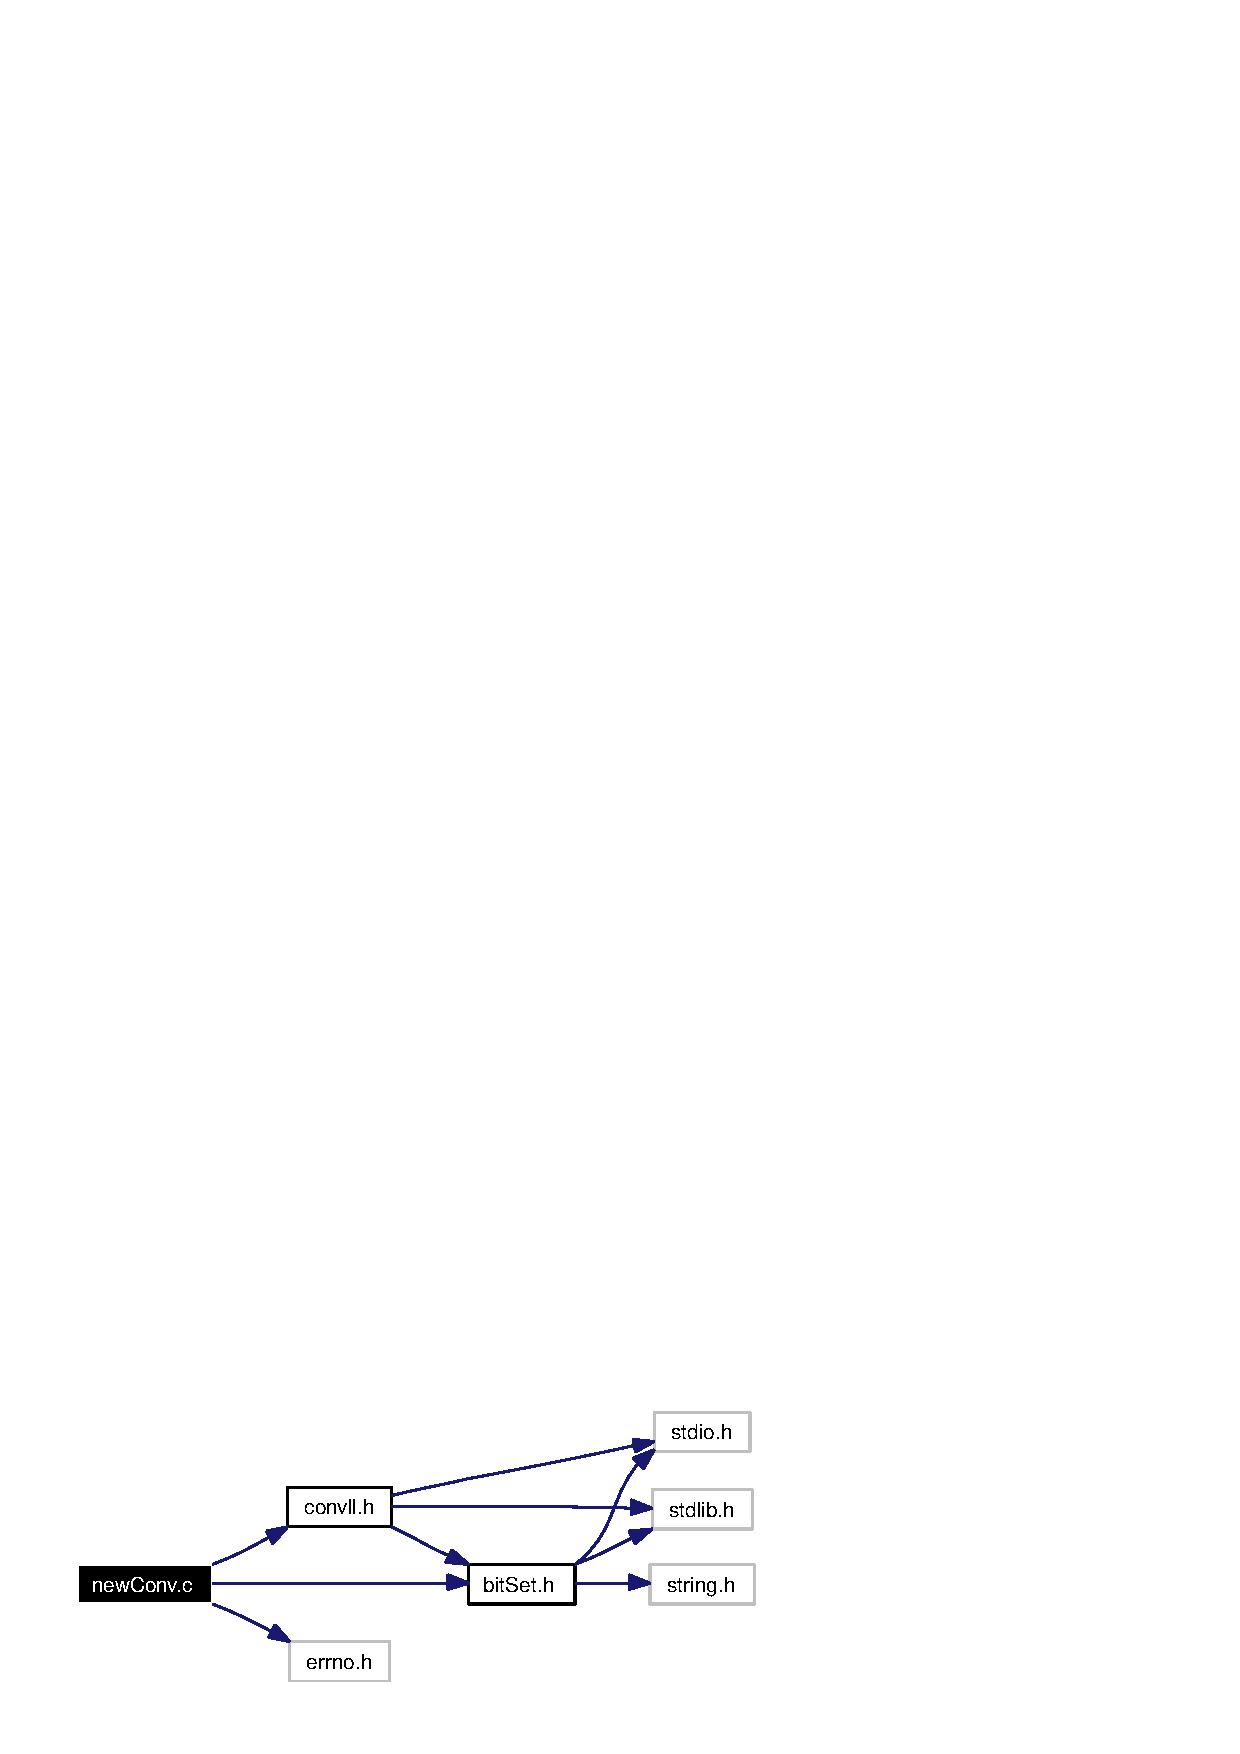
\includegraphics[width=181pt]{newConv_8c__incl}
\end{center}
\end{figure}
\subsection*{Functions}
\begin{CompactItemize}
\item 
int \hyperlink{newConv_8c_a0}{find\-Cliques} (\hyperlink{structbitSet__t}{bit\-Set\_\-t} $\ast$Q, \hyperlink{structbitSet__t}{bit\-Set\_\-t} $\ast$cand, \hyperlink{structbitSet__t}{bit\-Set\_\-t} $\ast$mask, \hyperlink{structbitGraph__t}{bit\-Graph\_\-t} $\ast$o\-G, int support, int q\-Count, \hyperlink{structcnode}{cll\_\-t} $\ast$$\ast$elem\-Pats, int $\ast$index\-To\-Seq, int p)
\item 
int \hyperlink{newConv_8c_a1}{single\-Linkage} (\hyperlink{structbitSet__t}{bit\-Set\_\-t} $\ast$Q, \hyperlink{structbitSet__t}{bit\-Set\_\-t} $\ast$cand, \hyperlink{structbitSet__t}{bit\-Set\_\-t} $\ast$mask, \hyperlink{structbitGraph__t}{bit\-Graph\_\-t} $\ast$o\-G, int support, int q\-Count, \hyperlink{structcnode}{cll\_\-t} $\ast$$\ast$elem\-Pats, int $\ast$index\-To\-Seq, int p)
\item 
int \hyperlink{newConv_8c_a2}{filter\-Iter} (\hyperlink{structbitGraph__t}{bit\-Graph\_\-t} $\ast$graph, int support, \hyperlink{structbitSet__t}{bit\-Set\_\-t} $\ast$changed, \hyperlink{structbitSet__t}{bit\-Set\_\-t} $\ast$work)
\item 
int \hyperlink{newConv_8c_a3}{filter\-Graph} (\hyperlink{structbitGraph__t}{bit\-Graph\_\-t} $\ast$graph, int support, int R)
\item 
\hyperlink{structbitGraph__t}{bit\-Graph\_\-t} $\ast$ \hyperlink{newConv_8c_a4}{prune\-Bit\-Graph} (\hyperlink{structbitGraph__t}{bit\-Graph\_\-t} $\ast$bg, int $\ast$index\-To\-Seq, int $\ast$$\ast$offset\-To\-Index, int num\-Of\-Seqs, int p)
\item 
\hyperlink{structcnode}{cll\_\-t} $\ast$ \hyperlink{newConv_8c_a5}{prune\-Cll} (\hyperlink{structcnode}{cll\_\-t} $\ast$head, int $\ast$index\-To\-Seq, int p)
\item 
\hyperlink{structcnode}{cll\_\-t} $\ast$ \hyperlink{newConv_8c_a6}{convolve} (\hyperlink{structbitGraph__t}{bit\-Graph\_\-t} $\ast$bg, int support, int R, int $\ast$index\-To\-Seq, int p, int cluster\-Method, int $\ast$$\ast$offset\-To\-Index, int number\-Of\-Sequences, int no\-Convolve, FILE $\ast$OUTPUT\_\-FILE)
\end{CompactItemize}


\subsection*{Detailed Description}
This file contains the core functions that performed the convolution in the Gemoda algorithm. As well, there are two clustering functions defined in this file: one for single linkage clustering, and one for clique based clustering.

Definition in file \hyperlink{newConv_8c-source}{new\-Conv.c}.

\subsection*{Function Documentation}
\hypertarget{newConv_8c_a6}{
\index{newConv.c@{new\-Conv.c}!convolve@{convolve}}
\index{convolve@{convolve}!newConv.c@{new\-Conv.c}}
\subsubsection[convolve]{\setlength{\rightskip}{0pt plus 5cm}\hyperlink{structcnode}{cll\_\-t}$\ast$ convolve (\hyperlink{structbitGraph__t}{bit\-Graph\_\-t} $\ast$ {\em bg}, int {\em support}, int {\em R}, int $\ast$ {\em index\-To\-Seq}, int {\em p}, int {\em cluster\-Method}, int $\ast$$\ast$ {\em offset\-To\-Index}, int {\em number\-Of\-Sequences}, int {\em no\-Convolve}, FILE $\ast$ {\em OUTPUT\_\-FILE})}}
\label{newConv_8c_a6}


Our outer convolution function. This function will call preliminary functions, cluster the data, and then call the main convolution function. This is the interface between the main gemoda-$<$x$>$ code and the generic code that gets all of the work done. Input: the bit\-Graph to be clustered and convolved, the minimum support necessary for a motif to be returned, a flag indicating whether recursive filtering should be used, a pointer to the data structure that dereferences offset indices to sequence numbers, the number of unique source sequences that a motif must be present in, and a number indicating the clustering method that is to be used. Output: the final motif linked list with all motifs that are to be given as output to the user.

Definition at line 625 of file new\-Conv.c.

References bit\-Graph\-Set\-False\-Diagonal(), complete\-Conv(), delete\-Bit\-Set(), fill\-Set(), filter\-Graph(), find\-Cliques(), new\-Bit\-Set(), prune\-Bit\-Graph(), prune\-Cll(), single\-Linkage(), bit\-Graph\_\-t::size, and yank\-Cll().

\scriptsize\begin{verbatim}629 {
630   bitSet_t * cand = NULL;
631   bitSet_t * mask = NULL;
632   bitSet_t * Q = NULL;
633   int size = bg->size;
634   cll_t * elemPats = NULL;
635   cll_t * allCliques = NULL;
636   cll_t * curr = NULL;
637   
638     // contains indices (rows) containing the threshold value.
639     cand = newBitSet (size);
640   mask = newBitSet (size);
641   Q = newBitSet (size);
642   fillSet (cand);
643   fillSet (mask);
644   
645     // Note that we prune based on p before setting the diagonal false.
646     if (p > 1)
647     {
648       bg =
649     pruneBitGraph (bg, indexToSeq, offsetToIndex, numberOfSequences, p);
650     }
651   
652     // Now we set the main diagonal false for clustering and filtering.
653     bitGraphSetFalseDiagonal (bg);
654   filterGraph (bg, support, R);
655   fprintf (OUTPUT_FILE, "Graph filtered!  Now clustering...\n");
656   fflush (NULL);
657   if (clusterMethod == 0)
658     {
659       findCliques (Q, cand, mask, bg, support, 0, &elemPats, indexToSeq, p);
660     }
661   else
662     {
663       singleLinkage (Q, cand, mask, bg, support, 0, &elemPats, indexToSeq,
664               p);
665     }
666   fprintf (OUTPUT_FILE,
667         "Clusters found!  Now filtering clusters (if option set)...\n");
668   fflush (NULL);
669   if (p > 1)
670     {
671       elemPats = pruneCll (elemPats, indexToSeq, p);
672     }
673   deleteBitSet (cand);
674   deleteBitSet (mask);
675   deleteBitSet (Q);
676   
677     // Now let's convolve what we made.
678     if (noConvolve == 0)
679     {
680       fprintf (OUTPUT_FILE, "Now convolving...\n");
681       fflush (NULL);
682       allCliques = completeConv (&elemPats, support, size, 0, indexToSeq, p);
683     }
684   
685   else
686     {
687       curr = elemPats;
688       while (curr != NULL)
689     {
690       yankCll (&elemPats, NULL, &curr, &allCliques, 0);
691     }
692     }
693   return allCliques;
694 }
\end{verbatim}
\normalsize 


\hypertarget{newConv_8c_a3}{
\index{newConv.c@{new\-Conv.c}!filterGraph@{filterGraph}}
\index{filterGraph@{filterGraph}!newConv.c@{new\-Conv.c}}
\subsubsection[filterGraph]{\setlength{\rightskip}{0pt plus 5cm}int filter\-Graph (\hyperlink{structbitGraph__t}{bit\-Graph\_\-t} $\ast$ {\em graph}, int {\em support}, int {\em R})}}
\label{newConv_8c_a3}


Function to \char`\"{}filter\char`\"{} the initial bit\-Graph that is being clustered. \char`\"{}Filtering\char`\"{} is the process of removing all nodes from the graph that cannot possibly be in motifs because they are not connected to enough other nodes. This can be done once (if R != 1), or it can be done recursively (if R == 1). When done recursively, it takes the just-filtered graph and checks all of the nodes that the recently removed node used to be connected to; since they have changed in connectivity, they may no longer be connected to enough nodes to be a member of a motif. This is iterated until convergence. Note that the default is to have recursive filtering on, as it ought to decrease the computational complexity of the clustering step and ought not have much of a computational footprint... in cases where it takes a while, it is probably having a good impact in the clustering step, whereas if it is not effective, it probably won't take that long anyway. Input: a bit\-Graph to be filtered, the minimum support that a motif must have, and the flag indicating recursive filtering or not. Output: Integer success value of 0 (and an altered bit\-Graph so that all nodes with connections have at least $<$min support$>$=\char`\"{}\char`\"{}$>$ connections).

Definition at line 359 of file new\-Conv.c.

References copy\-Set(), count\-Set(), delete\-Bit\-Set(), empty\-Set(), filter\-Iter(), new\-Bit\-Set(), and bit\-Graph\_\-t::size.

Referenced by convolve().

\scriptsize\begin{verbatim}360 {
361   bitSet_t * changed = newBitSet (graph->size);
362   bitSet_t * work = newBitSet (graph->size);
363   emptySet (changed);
364   emptySet (work);
365   
366     // Iteratively call the filtering by copying the previous "work" into
367     // "changed" after each iteration step.
368     if (R == 1)
369     {
370       
371       do
372     {
373       filterIter (graph, support, changed, work);
374       copySet (work, changed);
375     }
376       while (countSet (changed) > 0);
377     }
378   else
379     {
380       
381     // Otherwise, just do it once.
382     filterIter (graph, support, changed, work);
383     }
384   deleteBitSet (changed);
385   deleteBitSet (work);
386   return 0;
387 }
\end{verbatim}
\normalsize 


\hypertarget{newConv_8c_a2}{
\index{newConv.c@{new\-Conv.c}!filterIter@{filterIter}}
\index{filterIter@{filterIter}!newConv.c@{new\-Conv.c}}
\subsubsection[filterIter]{\setlength{\rightskip}{0pt plus 5cm}int filter\-Iter (\hyperlink{structbitGraph__t}{bit\-Graph\_\-t} $\ast$ {\em graph}, int {\em support}, \hyperlink{structbitSet__t}{bit\-Set\_\-t} $\ast$ {\em changed}, \hyperlink{structbitSet__t}{bit\-Set\_\-t} $\ast$ {\em work})}}
\label{newConv_8c_a2}


The iterator used to \char`\"{}filter\char`\"{} the graph. It takes information in the bitset telling which nodes' rows have changed and only checks them... this should make it pretty efficient time-wise at only a small memory cost. Note the convention that the first time this is called, the changed bit\-Set is empty... and that the master function is responsible for catching the signal that no changes were made in the last iteration. Input: the bit\-Graph to be filtered, the minimum support required for a motif to be returned, a bit\-Set with nodes changed from the previous iteration, and a bit\-Set to export the nodes changed in this iteration. Output: integer success value of 0 (and also a filtered bit\-Graph and a bit\-Set with the nodes changed in this iteration).

Definition at line 228 of file new\-Conv.c.

References count\-Set(), empty\-Set(), bit\-Graph\_\-t::graph, next\-Bit\-Bit\-Set(), set\-False(), and set\-True().

Referenced by filter\-Graph().

\scriptsize\begin{verbatim}230 {
231   int i = 0, j = 0;
232   int lastBit = 0, nextBit = 0, lastRow = 0, nextRow = 0;
233   int numNodes = 0;
234   int changedSize = countSet (changed);
235   emptySet (work);
236   
237     // Note the convention that the first time the function is called,
238     // it is done with an empty "changed" bitSet as a sentinel.  It is
239     // the responsibility of the master function calling the iterator
240     // to catch future empty changed sets to know that convergence has
241     // been achieved.
242     // 
243     // So, if it's your first time through, go through each node and make
244     // sure that each is connected to at least <support> - 1 others.
245     if (changedSize == 0)
246     {
247       for (i = 0; i < graph->size; i++)
248     {
249       numNodes = countSet (graph->graph[i]);
250       if (numNodes >= support - 1)
251         {
252           continue;
253         }
254       else
255         {
256           
257         // Otherwise, zero it out, but going one by
258         // one so that you can also zero out the 
259         // symmetric bit.
260         lastBit = 0;
261           for (j = 0; j < numNodes; j++)
262         {
263           nextBit = nextBitBitSet (graph->graph[i], lastBit);
264           if (nextBit == -1)
265             {
266               fprintf (stderr,
267                 "\nEnd of bitSet reached! - initial\n");
268               fflush (stderr);
269               exit (0);
270             }
271           setFalse (graph->graph[i], nextBit);
272           setFalse (graph->graph[nextBit], i);
273           
274             // And set that corresponding bit true
275             // in the work bitSet so that we
276             // know we changed it for the next
277             // round.
278             setTrue (work, nextBit);
279           lastBit = nextBit + 1;
280         }
281         }
282     }
283     }
284   else
285     {
286       
287     // Otherwise, we've been here before, so just follow what
288     // the changed bitSet says to do... only those bitSets that
289     // were changed could possibly have gone under the minimum
290     // support requirement.
291     lastRow = 0;
292       for (i = 0; i < changedSize; i++)
293     {
294       nextRow = nextBitBitSet (changed, lastRow);
295       if (nextRow == -1)
296         {
297           fprintf (stderr, "\nEnd of bitSet reached! - iter,row\n");
298           fflush (stderr);
299           exit (0);
300         }
301       
302         // So now we've found the row that needs to be checked.
303         // We do the same thing we did above... either move
304         // on if it has enough possible support, or zero
305         // it out (with its symmetric locations) one by one.
306         numNodes = countSet (graph->graph[nextRow]);
307       if (numNodes >= support - 1)
308         {
309           lastRow = nextRow + 1;
310           continue;
311         }
312       else
313         {
314           lastBit = 0;
315           for (j = 0; j < numNodes; j++)
316         {
317           nextBit = nextBitBitSet (graph->graph[nextRow], lastBit);
318           if (nextBit == -1)
319             {
320               fprintf (stderr,
321                 "\nEnd of BitSet reached! = iter,Bit\n");
322               fflush (stderr);
323               exit (0);
324             }
325           setFalse (graph->graph[nextRow], nextBit);
326           setFalse (graph->graph[nextBit], nextRow);
327           setTrue (work, nextBit);
328           lastBit = nextBit + 1;
329         }
330           lastRow = nextRow + 1;
331         }
332     }
333     }
334   return 1;
335 }
\end{verbatim}
\normalsize 


\hypertarget{newConv_8c_a0}{
\index{newConv.c@{new\-Conv.c}!findCliques@{findCliques}}
\index{findCliques@{findCliques}!newConv.c@{new\-Conv.c}}
\subsubsection[findCliques]{\setlength{\rightskip}{0pt plus 5cm}int find\-Cliques (\hyperlink{structbitSet__t}{bit\-Set\_\-t} $\ast$ {\em Q}, \hyperlink{structbitSet__t}{bit\-Set\_\-t} $\ast$ {\em cand}, \hyperlink{structbitSet__t}{bit\-Set\_\-t} $\ast$ {\em mask}, \hyperlink{structbitGraph__t}{bit\-Graph\_\-t} $\ast$ {\em o\-G}, int {\em support}, int {\em q\-Count}, \hyperlink{structcnode}{cll\_\-t} $\ast$$\ast$ {\em elem\-Pats}, int $\ast$ {\em index\-To\-Seq}, int {\em p})}}
\label{newConv_8c_a0}


Recursive algorithm to exhaustively enumerate all of the maximal cliques that exist in the data. This is one of the main workhorses of Gemoda when used in its exhaustive form. This algorithm was originally published by Etsuji Tomita, Akira Tanaka, and Haruhisa Takahasi as a Technical Report of IPSJ (Information Processing Society of Japan): Tomita, E, A Tanaka, \& H Takahasi (1989). \char`\"{}An optimal algorithm for finding all of the cliques\char`\"{}. SIG Algorithms 12, pp 91-98. Input: a bitset with the nodes currently in the clique, a bitset with the candidates for expanding the clique, a bitset inidcating the current subgraph being searched, the bit\-Graph to be searched for cliques, the minimum support parameter, a counter variable for keeping track of how many nodes are in the current clique, a linked list of cliques that have been discovered so far, and a pointer to the data structure that dereferences offset indexes into sequence numbers, and the minimum number of unique sequences that must contain the motif. Output: integer success value of 0 (but more importantly, the elem\-Pats clique linked list is expanded to contain all elementary (minimum-length) motif cliques.

Definition at line 37 of file new\-Conv.c.

References bit\-Set\-Intersection(), check\-Bit(), count\-Set(), delete\-Bit\-Set(), bit\-Graph\_\-t::graph, new\-Bit\-Set(), next\-Bit\-Bit\-Set(), push\-Clique(), set\-False(), set\-True(), and bit\-Graph\_\-t::size.

Referenced by convolve().

\scriptsize\begin{verbatim}40 {
41   bitSet_t ** gammaOG = NULL;
42   bitSet_t * candQ = newBitSet (oG->size);
43   bitSet_t * newMask = newBitSet (oG->size);
44   int i, q;
45   int graphSize;
46   int max = -1;
47   int numBits;
48   int u = 0;
49   int newMaskCount;
50   int candQCount;
51   graphSize = oG->size;
52   
53     // 
54     // Find which vertex in subg maximizes |cand intersect gamma(u) |
55     gammaOG = oG->graph;
56   for (i = 0; i < graphSize; i++)
57     {
58       
59     // Don't check this vertex if it's masked
60     if (!(checkBit (mask, i)))
61     {
62       continue;
63     }
64       
65     // cand is always a subset of mask, so intersecting
66     // with mask is redundant
67     bitSetIntersection (gammaOG[i], cand, candQ);
68       numBits = countSet (candQ);
69       if (numBits > max)
70     {
71       u = i;
72       max = numBits;
73     }
74     }
75   
76     // Then do the extension of the q's
77     qCount++;
78   
79     // This loop iterates over all possible values of cand - gamma() by
80     // iterating over all possible values of cand but immediately
81     // "continue"ing if the node is also in gamma(u)
82     q = nextBitBitSet (cand, 0);
83   while (q != -1)
84     {
85       if (checkBit (gammaOG[u], q))
86     {
87       q = nextBitBitSet (cand, q + 1);
88       continue;
89     }
90       
91     // SUBGq = SUBG i Gamma
92     bitSetIntersection (mask, gammaOG[q], newMask);
93       newMaskCount = countSet (newMask);
94       setTrue (Q, q);
95       
96     // Only recurse if there are more candidates to be included,
97     // and they will allow us to reach the minimum support. 
98     if (newMaskCount > 0 && qCount + newMaskCount >= support)
99     {
100       
101         // CANDq = CAND i Gamma
102         bitSetIntersection (gammaOG[q], cand, candQ);
103       candQCount = countSet (candQ);
104       
105         // only recurse if we can possibly get to a clique
106         // of size with minimum support
107         if (candQCount > 0 && qCount + candQCount >= support)
108         {
109           
110         // recursion with
111         // new candidates, new mask, and original graph
112         findCliques (Q, candQ, newMask, oG, support, qCount, elemPats,
113                  indexToSeq, p);
114         }
115     }
116       else if (qCount >= support)
117     {
118       
119         // This should be done when:
120         // 1. countSet(newMask) == 0 [connected subgraph is maximal]
121         // 2. Qcount >= minCount [connected subgraph has enough nodes]
122         *elemPats = pushClique (Q, *elemPats, indexToSeq, p);
123     }
124       
125     // Remove q from Q, and remove q from cand
126     setFalse (Q, q);
127       setFalse (cand, q);
128       q = nextBitBitSet (cand, q + 1);
129     }
130   qCount--;
131   deleteBitSet (candQ);
132   deleteBitSet (newMask);
133   return 0;
134 }
\end{verbatim}
\normalsize 


\hypertarget{newConv_8c_a4}{
\index{newConv.c@{new\-Conv.c}!pruneBitGraph@{pruneBitGraph}}
\index{pruneBitGraph@{pruneBitGraph}!newConv.c@{new\-Conv.c}}
\subsubsection[pruneBitGraph]{\setlength{\rightskip}{0pt plus 5cm}\hyperlink{structbitGraph__t}{bit\-Graph\_\-t}$\ast$ prune\-Bit\-Graph (\hyperlink{structbitGraph__t}{bit\-Graph\_\-t} $\ast$ {\em bg}, int $\ast$ {\em index\-To\-Seq}, int $\ast$$\ast$ {\em offset\-To\-Index}, int {\em num\-Of\-Seqs}, int {\em p})}}
\label{newConv_8c_a4}


Simple function (non-recursive) to prune off the first level of motifs that will not meet the \char`\"{}minimum number of unique sequences\char`\"{} criterion. This could have been implemented as above, but it may have gotten a little expensive with less yield, so only the first run through is done here. Input: a bit graph to be pruned, a pointer to the structure that dereferences offset indices to sequence numbers, a pointer to the structure that dereferences seq/position to offsets, the number of unique sequences in the input set, and the minimum number of unique sequences that must contain the motif. Output: a pruned bit\-Graph.

Definition at line 402 of file new\-Conv.c.

References empty\-Set(), bit\-Graph\_\-t::graph, and next\-Bit\-Bit\-Set().

\scriptsize\begin{verbatim}404 {
405   int i = 0, j = 0, nextBit = 0;
406   int *seqNums = NULL;
407   
408     // Since we don't immediately know which node is in which source 
409     // sequence, we can't just count them up regularly.  Instead, we'll
410     // need to keep track of which sequences they come from and 
411     // increment _something_.  What we chose to do here is just make
412     // an array of integers of length = <p>.  Then, we try to put the
413     // source sequence number of each neighbor (including itself, since
414     // the main diagonal is still true at this time) into the next slot
415     // Since we will monotonically search the bitSet, we can just 
416     // move on to the first bit in the next sequence using the 
417     // offsetToIndex structure so that we know the next sequence number
418     // to be put in is always unique.
419     seqNums = (int *) malloc (p * sizeof (int));
420   if (seqNums == NULL)
421     {
422       fprintf (stderr, "Memory error - pruneBitGraph\n%s\n",
423         strerror (errno));
424       fflush (stderr);
425       exit (0);
426     }
427   
428     // So, for each row in the bitgraph...
429     for (i = 0; i < bg->size; i++)
430     {
431       
432     // Make sure the whole array is -1 sentinels.
433     for (j = 0; j < p; j++)
434     {
435       seqNums[j] = -1;
436     }
437       j = 0;
438       
439     // Find the first neighbor of this bit.
440     nextBit = nextBitBitSet (bg->graph[i], 0);
441       if (nextBit == -1)
442     {
443       continue;
444     }
445       else
446     {
447       
448         // and put its sequence number in the array of ints.
449         seqNums[0] = indexToSeq[nextBit];
450     }
451       
452     // If it's the last sequence, then bail out so that we don't
453     // segfault in the next step.
454     if (seqNums[0] >= numOfSeqs - 1)
455     {
456       emptySet (bg->graph[i]);
457       continue;
458     }
459       
460     // Find the next neighbor of this bit, STARTING AT the first
461     // bit in the next sequence.
462     nextBit =
463     nextBitBitSet (bg->graph[i],
464                offsetToIndex[indexToSeq[nextBit] + 1][0]);
465       
466     // And iterate this until we run out of neighbors.
467     while (nextBit >= 0)
468     {
469       j++;
470       seqNums[j] = indexToSeq[nextBit];
471       
472         // Or until this new neighbor will fill up the array
473         if (j == p - 1)
474         {
475           break;
476         }
477       
478         // Or until this new neighbor is in the last sequence.
479         if (seqNums[j] >= numOfSeqs - 1)
480         {
481           break;
482         }
483       
484         // Get the next neighbor!
485         nextBit =
486         nextBitBitSet (bg->graph[i],
487                offsetToIndex[indexToSeq[nextBit] + 1][0]);
488     }
489       
490     // If we didn't have enough unique sequences, and either a) we
491     // were in the nth-to-last sequence and there were no 
492     // neighbors after it, or b) we were in the last sequence,
493     // then the last number will still be our sentinel, -1.  If
494     // the last number is not a sentinel, then we have at least
495     // p distinct sequence occurrences, so we're OK.
496     if (seqNums[p - 1] == -1)
497     {
498       emptySet (bg->graph[i]);
499     }
500     }
501   free (seqNums);
502   return (bg);
503 }
\end{verbatim}
\normalsize 


\hypertarget{newConv_8c_a5}{
\index{newConv.c@{new\-Conv.c}!pruneCll@{pruneCll}}
\index{pruneCll@{pruneCll}!newConv.c@{new\-Conv.c}}
\subsubsection[pruneCll]{\setlength{\rightskip}{0pt plus 5cm}\hyperlink{structcnode}{cll\_\-t}$\ast$ prune\-Cll (\hyperlink{structcnode}{cll\_\-t} $\ast$ {\em head}, int $\ast$ {\em index\-To\-Seq}, int {\em p})}}
\label{newConv_8c_a5}


Prunes a motif linked list of all motifs without support in at least

unique source sequences. Input: head of a motif linked list, pointer to a structure that dereferences offset indices to sequence numbers, minimum number of unique source sequences in which a motif must occur. Output: head of a (potentially altered) motif linked list.

Definition at line 514 of file new\-Conv.c.

References c\-Set\_\-t::members, cnode::next, cnode::set, and c\-Set\_\-t::size.

Referenced by complete\-Conv(), and convolve().

\scriptsize\begin{verbatim}515 {
516   int i = 0, j = 0, thisSeq = 0;
517   int *seqNums = NULL;
518   cll_t * curr = head;
519   cll_t * prev = NULL;
520   cll_t * storage = NULL;
521   
522     // We'll do this similar to the pruneBitGraph function... we will
523     // keep track of which source sequence each motif occurrence was in.
524     // Again, since the occurrences are listed monotonically, we only
525     // need to compare the last non-sentinel index to the current
526     // sequence number.
527     seqNums = (int *) malloc (p * sizeof (int));
528   if (seqNums == NULL)
529     {
530       fprintf (stderr, "Memory error - pruneCll\n%s\n", strerror (errno));
531       fflush (stderr);
532       exit (0);
533     }
534   while (curr != NULL)
535     {
536       
537     // First make sure the set size is at least p.
538     // This is redundant, but extremely simple and not expensive,
539     // so we'll leave it in just as a check.
540     if (curr->set->size < p)
541     {
542       if (prev != NULL)
543         {
544           prev->next = curr->next;
545         }
546       else
547         {
548           head = curr->next;
549         }
550       storage = curr->next;
551       free (curr->set->members);
552       free (curr->set);
553       free (curr);
554       curr = storage;
555       continue;
556     }
557       for (i = 0; i < p; i++)
558     {
559       seqNums[i] = -1;
560     }
561       j = 0;
562       seqNums[0] = indexToSeq[curr->set->members[0]];
563       
564     // Note, we've checked to make sure size > p, and we know
565     // p must be 2 or greater, so we can start at 1 without
566     // worrying about segfaulting
567     for (i = 1; i < curr->set->size; i++)
568     {
569       thisSeq = indexToSeq[curr->set->members[i]];
570       if (thisSeq != seqNums[j])
571         {
572           j++;
573           seqNums[j] = thisSeq;
574           if (j == p - 1)
575         {
576           break;
577         }
578         }
579     }
580       
581     // Same story as before... if the last number is -1,
582     // then we didn't have enough to fill up the <p> different
583     // slots, so this doesn't meet our criterion.
584     if (seqNums[p - 1] == -1)
585     {
586       if (prev != NULL)
587         {
588           prev->next = curr->next;
589         }
590       else
591         {
592           head = curr->next;
593         }
594       storage = curr->next;
595       free (curr->set->members);
596       free (curr->set);
597       free (curr);
598       curr = storage;
599     }
600       else
601     {
602       prev = curr;
603       curr = curr->next;
604     }
605     }
606   free (seqNums);
607   return (head);
608 }
\end{verbatim}
\normalsize 


\hypertarget{newConv_8c_a1}{
\index{newConv.c@{new\-Conv.c}!singleLinkage@{singleLinkage}}
\index{singleLinkage@{singleLinkage}!newConv.c@{new\-Conv.c}}
\subsubsection[singleLinkage]{\setlength{\rightskip}{0pt plus 5cm}int single\-Linkage (\hyperlink{structbitSet__t}{bit\-Set\_\-t} $\ast$ {\em Q}, \hyperlink{structbitSet__t}{bit\-Set\_\-t} $\ast$ {\em cand}, \hyperlink{structbitSet__t}{bit\-Set\_\-t} $\ast$ {\em mask}, \hyperlink{structbitGraph__t}{bit\-Graph\_\-t} $\ast$ {\em o\-G}, int {\em support}, int {\em q\-Count}, \hyperlink{structcnode}{cll\_\-t} $\ast$$\ast$ {\em elem\-Pats}, int $\ast$ {\em index\-To\-Seq}, int {\em p})}}
\label{newConv_8c_a1}


A recursive routine for single linkage clustering. This clustering is much faster than exhaustively enumerating all cliques, but it puts each node in only one cluster and is not guaranteed to give all possible motifs. Input: a bit\-Set containing the current motif, a bit\-Set containing candidates to be added to the current motif, a bit\-Set containing the current subgraph to be clustered, the original bit\-Graph to be clustered, the minimum support necessary for a motif to be returned, the current number of nodes in the motif, a linked list of elementary motifs (length is the same as the window size), pointer to a structure to derference index values to sequence numbers, and the minimum number of unique sequences that a motif must be in to be returned. Output: integer success value of 0 (but more importantly, the linked list elem\-Pats is updated to contain all of the motifs of length = window size.

Definition at line 154 of file new\-Conv.c.

References bit\-Set\-Union(), check\-Bit(), copy\-Set(), count\-Set(), bit\-Graph\_\-t::graph, next\-Bit\-Bit\-Set(), push\-Clique(), and set\-False().

Referenced by convolve().

\scriptsize\begin{verbatim}157 {
158   int i = 0;
159   int j = 0;
160   
161     // go to the first vertex that has not been clustered yet
162     i = nextBitBitSet (cand, 0);
163   if (i != -1)
164     {
165       
166     // this vertex has been clustered
167     setFalse (cand, i);
168       
169     // start a new cluster, Q
170     copySet (oG->graph[i], Q);
171       
172     // go over each vertex in the cluster
173     j = nextBitBitSet (Q, 0);
174       while (j != -1)
175     {
176       
177         // if this vertex has been clustered already, skip it and go
178         // to the next one
179         if (!checkBit (cand, j))
180         {
181           j = nextBitBitSet (Q, j + 1);
182           continue;
183         }
184       
185         // Add this vertex's neighbors to the current cluster
186         bitSetUnion (Q, oG->graph[j], Q);
187       
188         // This vertex has now been clustered
189         setFalse (cand, j);
190       
191         // go over each vertex in the cluster
192         j = nextBitBitSet (Q, 0);
193     }
194       
195     // Did we make a cluster that was large enough?
196     if (countSet (Q) >= support)
197     {
198       *elemPats = pushClique (Q, *elemPats, indexToSeq, p);
199     }
200       
201     // recurse
202     singleLinkage (Q, cand, mask, oG, support, 0, elemPats, indexToSeq,
203                p);
204     }
205   else
206     {
207       return 0;
208     }
209   return 0;
210 }
\end{verbatim}
\normalsize 



\hypertarget{patStats_8c}{
\section{pat\-Stats.c File Reference}
\label{patStats_8c}\index{patStats.c@{patStats.c}}
}
{\tt \#include $<$math.h$>$}\par
{\tt \#include \char`\"{}pat\-Stats.h\char`\"{}}\par


Include dependency graph for pat\-Stats.c:\begin{figure}[H]
\begin{center}
\leavevmode
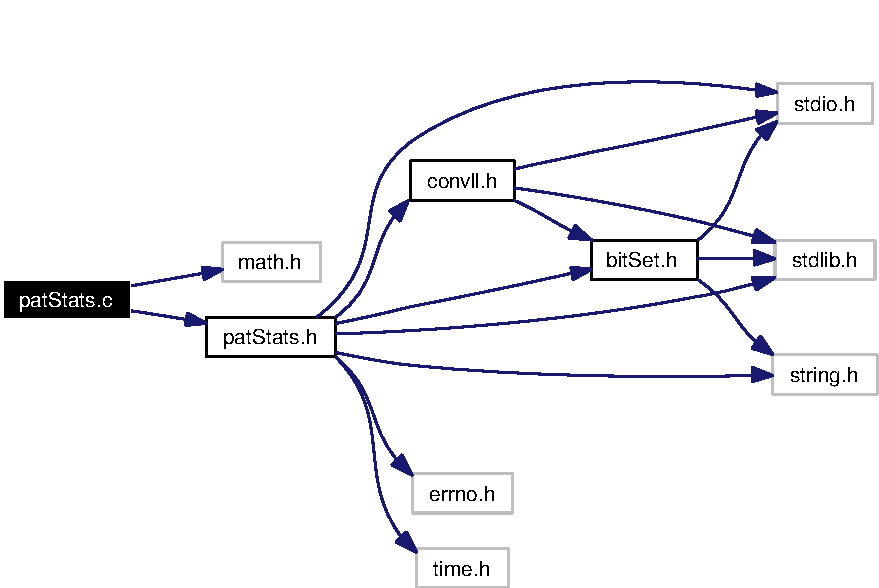
\includegraphics[width=228pt]{patStats_8c__incl}
\end{center}
\end{figure}
\subsection*{Functions}
\begin{CompactItemize}
\item 
int \hyperlink{patStats_8c_a0}{get\-Largest\-Support} (\hyperlink{structcnode}{cll\_\-t} $\ast$cliqs)
\item 
int \hyperlink{patStats_8c_a1}{get\-Largest\-Length} (\hyperlink{structcnode}{cll\_\-t} $\ast$cliqs)
\item 
int \hyperlink{patStats_8c_a2}{measure\-Diagonal} (const \hyperlink{structbitGraph__t}{bit\-Graph\_\-t} $\ast$bg, const int i, const int j)
\item 
unsigned int $\ast$$\ast$ \hyperlink{patStats_8c_a3}{increase\-Mem} (unsigned int $\ast$$\ast$d, int dim\-To\-Change, int curr\-Support, int curr\-Length, int new\-Val)
\item 
unsigned int $\ast$$\ast$ \hyperlink{patStats_8c_a4}{old\-Get\-Stat\-Mat} (\hyperlink{structbitGraph__t}{bit\-Graph\_\-t} $\ast$bg, int support, int length, int $\ast$support\-Dim, int $\ast$length\-Dim, int num\-Blanks)
\item 
unsigned int $\ast$$\ast$ \hyperlink{patStats_8c_a5}{get\-Stat\-Mat} (\hyperlink{structbitGraph__t}{bit\-Graph\_\-t} $\ast$bg, int support, int length, int $\ast$support\-Dim, int $\ast$length\-Dim, int num\-Blanks, int s, FILE $\ast$OUTPUT\_\-FILE)
\item 
int \hyperlink{patStats_8c_a6}{cum\-DMatrix} (unsigned int $\ast$$\ast$d, \hyperlink{structcnode}{cll\_\-t} $\ast$cliqs, int curr\-Support, int curr\-Length, int bg\-Size, int num\-Seqs)
\item 
double \hyperlink{patStats_8c_a7}{calc\-Stat\-Cliq} (unsigned int $\ast$$\ast$d, \hyperlink{structcnode}{cll\_\-t} $\ast$cliq, int num\-Windows)
\item 
int \hyperlink{patStats_8c_a8}{calc\-Stat\-All\-Cliqs} (unsigned int $\ast$$\ast$d, \hyperlink{structcnode}{cll\_\-t} $\ast$all\-Cliqs, int num\-Windows)
\item 
int \hyperlink{patStats_8c_a9}{free\-D} (unsigned int $\ast$$\ast$d, int support\-Dim)
\item 
int \hyperlink{patStats_8c_a10}{stat\-Compare} (const \hyperlink{structcnode}{cll\_\-t} $\ast$$\ast$first, const \hyperlink{structcnode}{cll\_\-t} $\ast$$\ast$second)
\item 
\hyperlink{structcnode}{cll\_\-t} $\ast$ \hyperlink{patStats_8c_a11}{sort\-By\-Stats} (\hyperlink{structcnode}{cll\_\-t} $\ast$all\-Cliqs)
\end{CompactItemize}


\subsection*{Detailed Description}
This file defines functions that are used to compute the statistical significance of motifs for both the sequence based and real value based implementations of Gemoda. The basic approach we take, is to calculate the probability of establishing a single cluster, and to multiply this probability by the probability that the cluster can be extended an arbitrary number of locations. Essentially, this is the probability of getting and elementary motif during the clustering phase and having that motif convolved multiple times during the convolution phase.

Definition in file \hyperlink{patStats_8c-source}{pat\-Stats.c}.

\subsection*{Function Documentation}
\hypertarget{patStats_8c_a8}{
\index{patStats.c@{pat\-Stats.c}!calcStatAllCliqs@{calcStatAllCliqs}}
\index{calcStatAllCliqs@{calcStatAllCliqs}!patStats.c@{pat\-Stats.c}}
\subsubsection[calcStatAllCliqs]{\setlength{\rightskip}{0pt plus 5cm}int calc\-Stat\-All\-Cliqs (unsigned int $\ast$$\ast$ {\em d}, \hyperlink{structcnode}{cll\_\-t} $\ast$ {\em all\-Cliqs}, int {\em num\-Windows})}}
\label{patStats_8c_a8}




Definition at line 676 of file pat\-Stats.c.

References calc\-Stat\-Cliq(), cnode::next, and cnode::stat.

Referenced by main().

\scriptsize\begin{verbatim}677 {
678   cll_t * curr = NULL;
679   curr = allCliqs;
680   while (curr != NULL)
681     {
682       curr->stat = calcStatCliq (d, curr, numWindows);
683       curr = curr->next;
684     }
685   return (0);
686 }
\end{verbatim}
\normalsize 


\hypertarget{patStats_8c_a7}{
\index{patStats.c@{pat\-Stats.c}!calcStatCliq@{calcStatCliq}}
\index{calcStatCliq@{calcStatCliq}!patStats.c@{pat\-Stats.c}}
\subsubsection[calcStatCliq]{\setlength{\rightskip}{0pt plus 5cm}double calc\-Stat\-Cliq (unsigned int $\ast$$\ast$ {\em d}, \hyperlink{structcnode}{cll\_\-t} $\ast$ {\em cliq}, int {\em num\-Windows})}}
\label{patStats_8c_a7}




Definition at line 623 of file pat\-Stats.c.

References cnode::length, cnode::set, and c\-Set\_\-t::size.

Referenced by calc\-Stat\-All\-Cliqs().

\scriptsize\begin{verbatim}624 {
625   double stat = 0;
626   int i = 0;
627   int supChooseTwo = 0;
628   double interimP = 0;
629   int support = cliq->set->size;
630   int length = cliq->length;
631   double numTrials = 0;
632   if (support < 2)
633     {
634       fprintf (stderr, "Support for cluster less than 2... exiting.\n");
635       fflush (stderr);
636       exit (0);
637     }
638   
639     // OK, so support is at least two.  So we make the connections all
640     // on the first level, knowing that each node being connected has
641     // at least zero in common.  There are [(size of cluster) - 1] of
642     // these connections to be made.
643     // And we know we can call for d[0][1] because if the second index
644     // were out of bounds, then there would be no similarities, and
645     // there would be no reason to call this function.
646     interimP = ((double) d[0][1]) / ((double) d[0][0]);
647   stat = pow (interimP, support - 1);
648   stat *= ((double) numWindows * (numWindows - 1)) / ((double) 2);
649   
650     // Now we actually calculate the probability... the first connection
651     // has to be made no matter what, and after that we multiply for 
652     // every connection after the first one.  So we descend iteratively
653     // until we have made all connections, terminating after we've made
654     // the single i = (n - 2) connection.  There is no i = (n - 1) 
655     // connection.
656     for (i = 1; i < support - 1; i++)
657     {
658       interimP = ((double) d[i][1]) / ((double) d[i][0]);
659       stat *= pow (interimP, support - i - 1);
660       stat *= ((double) (numWindows - (i + 1))) / ((double) (i + 2));
661     } supChooseTwo = (support * (support - 1)) / 2;
662   
663     // Remember that length = (numwindows - 1), or alternatively,
664     // the number of extensions... normally we'd want to have the last
665     // p be p[support][numwindows - 1], which corresponds to 
666     // alteredD[support][numwindows]/alteredD[support][numwindows-1],
667     // so that means we want our last d to be d[support][numwindows].
668     // Here, we note that the calculation of p's would be continuously
669     // re-normalizing, so multiplying all p's is the same as dividing
670     // the last d by the initial d.
671     interimP = ((double) d[support][length + 1]) / ((double) d[support][1]);
672   stat *= pow (interimP, supChooseTwo);
673   return stat;
674 }
\end{verbatim}
\normalsize 


\hypertarget{patStats_8c_a6}{
\index{patStats.c@{pat\-Stats.c}!cumDMatrix@{cumDMatrix}}
\index{cumDMatrix@{cumDMatrix}!patStats.c@{pat\-Stats.c}}
\subsubsection[cumDMatrix]{\setlength{\rightskip}{0pt plus 5cm}int cum\-DMatrix (unsigned int $\ast$$\ast$ {\em d}, \hyperlink{structcnode}{cll\_\-t} $\ast$ {\em cliqs}, int {\em curr\-Support}, int {\em curr\-Length}, int {\em bg\-Size}, int {\em num\-Seqs})}}
\label{patStats_8c_a6}




Definition at line 522 of file pat\-Stats.c.

References get\-Largest\-Length(), and get\-Largest\-Support().

Referenced by main().

\scriptsize\begin{verbatim}524 {
525   int maxSup = 0;
526   int maxLen = 0;
527   int i, j;
528   int numWins = 0;
529   
530     maxSup = getLargestSupport (cliqs);
531   maxLen = getLargestLength (cliqs);
532   
533 /********* COMMENTED OUT
534     // First we note that the number of unique streaks of a given
535     //  support is defined by d[support][1], where as 1 increases,
536     //  the value of d decreases because only unique streaks are
537     //  counted.
538     // We also note that the number of disjoint node-pairs with a given
539     //  number of other nodes in common is defined by d[support][0].
540     // So, in order to properly account for all "unique" comparisons 
541     //  (which is equal to (# streaks + # disjoint node-pairs), we must
542     //  add d[support][1] to d[support][0].
543     
544     for (i = 0; i < currSupport + 1; i++) {
545         d[i][0] += d[i][1];
546     }
547     ********************/ 
548     
549     // We no longer need to do that, since now we sum across both
550     // the support and the length dimensions.  Now, d[support][0] will
551     // necessarily include d[support][1] being added to it.  We don't 
552     // want to add this anymore, otherwise we would be underestimating
553     // the probability of making that first connection.  For instance,
554     // if there were no nodes with 20 in common that weren't also 
555     // connected, and no nodes whatsoever with more than 20 in common,
556     // we'd want the p[20][0] to be 1, which would be 
557     // d[20][1]/d[20][0].  When summing across length directions,
558     // this happens naturally, whereas before we needed to do it 
559     // artificially as per above.  If we did above, we'd have the
560     // probability of each node being 1/2 instead of 1.
561     
562     // Rather than storing doubles and doing lots of multiplications,
563     // we're going to limit the number of operations done in the actual
564     // probability calculation by only storing cumulative sums in d.
565     // Now remember, what we're storing at each location is the 
566     // number of nodes with [i] or more nodes in common (including
567     // each other and selves) that can be extended [j] times (with
568     // their initial similarity counting as 1).
569     // 
570     // We go up to the last possible index in the length direction, which
571     // means going up to [maxLen].  We know that this is legitimate
572     // because maxLen is less than or equal to the longest possible 
573     // diagonal, and the longest possible diagonal will be less
574     // than or equal to currLength.  Since we have allotted 
575     // (currLength + 1) integers, we know we're OK to access [currLength].
576     for (j = 0; j < currLength + 1; j++)
577     {
578       
579     // We start at currSupport - 1, because currSupport will
580     // clearly not be changed, and this makes it a much easier
581     // loop to read.
582     for (i = currSupport - 1; i >= 0; i--)
583     {
584       d[i][j] += d[i + 1][j];
585     }
586     }
587   for (i = 0; i < currSupport + 1; i++)
588     {
589       for (j = currLength - 1; j >= 0; j--)
590     {
591       d[i][j] += d[i][j + 1];
592     }
593     }
594   
595     // Now we need to forcibly set d[0][0] to its correct value... it's 
596     // just the total number of comparisons, not including comparisons
597     // to delimiter 0's meant to separate sequences.  The number of 
598     // windows is equal to the number of offsets minus the number
599     // of sequences (assuming one delimiter per sequence).  We don't count
600     // the main diagonal, so the first row has one less, and we want to
601     // sum over all the subsequent rows in the upper half of the matrix.
602     // So it's (numWins - 1)*(numWins - 1 + 1)/2 to sum that up.
603     numWins = bgSize - numSeqs;
604   d[0][0] = numWins * (numWins - 1) / 2;
605   
606     /*
607         for (i = 0; i <= maxSup; i++) { printf("support = %d:\t",i); for (j = 0; j <=
608        maxLen; j++) { printf("%d\t",d[i][j]); } printf("\n"); } 
609      */ 
610     return 1;
611 }
\end{verbatim}
\normalsize 


\hypertarget{patStats_8c_a9}{
\index{patStats.c@{pat\-Stats.c}!freeD@{freeD}}
\index{freeD@{freeD}!patStats.c@{pat\-Stats.c}}
\subsubsection[freeD]{\setlength{\rightskip}{0pt plus 5cm}int free\-D (unsigned int $\ast$$\ast$ {\em d}, int {\em support\-Dim})}}
\label{patStats_8c_a9}




Definition at line 688 of file pat\-Stats.c.

Referenced by main().

\scriptsize\begin{verbatim}689 {
690   int i = 0;
691   if (d == 0)
692     {
693       return 0;
694     }
695   else
696     {
697       
698     // Still, it's supportDim + 1, because we have an extra
699     // one for the "0" support.
700     for (i = 0; i < supportDim + 1; i++)
701     {
702       free (d[i]);
703     }
704       free (d);
705       return 0;
706     }
707 }
\end{verbatim}
\normalsize 


\hypertarget{patStats_8c_a1}{
\index{patStats.c@{pat\-Stats.c}!getLargestLength@{getLargestLength}}
\index{getLargestLength@{getLargestLength}!patStats.c@{pat\-Stats.c}}
\subsubsection[getLargestLength]{\setlength{\rightskip}{0pt plus 5cm}int get\-Largest\-Length (\hyperlink{structcnode}{cll\_\-t} $\ast$ {\em cliqs})}}
\label{patStats_8c_a1}


Given a clique linked list, this function will return an integer which is equal to the length of the member of the linked list with the largest length.

Definition at line 44 of file pat\-Stats.c.

References cnode::length, and cnode::next.

Referenced by cum\-DMatrix().

\scriptsize\begin{verbatim}45 {
46   int len = 0;
47   cll_t * curCliq = NULL;
48   curCliq = cliqs;
49   while (curCliq != NULL)
50     {
51       if (curCliq->length > len)
52     {
53       len = curCliq->length;
54     }
55       curCliq = curCliq->next;
56     }
57   
58     // We return (len + 1) because the length of the shortest streak
59     // is one, but is stored in the cluster data structure as being
60     // zero (number of extensions that have been made).
61     return (len + 1);
62 }
\end{verbatim}
\normalsize 


\hypertarget{patStats_8c_a0}{
\index{patStats.c@{pat\-Stats.c}!getLargestSupport@{getLargestSupport}}
\index{getLargestSupport@{getLargestSupport}!patStats.c@{pat\-Stats.c}}
\subsubsection[getLargestSupport]{\setlength{\rightskip}{0pt plus 5cm}int get\-Largest\-Support (\hyperlink{structcnode}{cll\_\-t} $\ast$ {\em cliqs})}}
\label{patStats_8c_a0}


Given a clique linked list, this function will return an integer which is equal to the support of the member of the linked list with the largest support.

Definition at line 22 of file pat\-Stats.c.

References cnode::next, cnode::set, and c\-Set\_\-t::size.

Referenced by cum\-DMatrix().

\scriptsize\begin{verbatim}23 {
24   int size = 0;
25   cll_t * curCliq = NULL;
26   curCliq = cliqs;
27   while (curCliq != NULL)
28     {
29       if (curCliq->set->size > size)
30     {
31       size = curCliq->set->size;
32     }
33       curCliq = curCliq->next;
34     }
35   return size;
36 }
\end{verbatim}
\normalsize 


\hypertarget{patStats_8c_a5}{
\index{patStats.c@{pat\-Stats.c}!getStatMat@{getStatMat}}
\index{getStatMat@{getStatMat}!patStats.c@{pat\-Stats.c}}
\subsubsection[getStatMat]{\setlength{\rightskip}{0pt plus 5cm}unsigned int$\ast$$\ast$ get\-Stat\-Mat (\hyperlink{structbitGraph__t}{bit\-Graph\_\-t} $\ast$ {\em bg}, int {\em support}, int {\em length}, int $\ast$ {\em support\-Dim}, int $\ast$ {\em length\-Dim}, int {\em num\-Blanks}, int {\em s}, FILE $\ast$ {\em OUTPUT\_\-FILE})}}
\label{patStats_8c_a5}




Definition at line 329 of file pat\-Stats.c.

References bit\-Graph\-Row\-Intersection(), check\-Bit(), count\-Set(), delete\-Bit\-Set(), bit\-Graph\_\-t::graph, increase\-Mem(), measure\-Diagonal(), new\-Bit\-Set(), next\-Bit\-Bit\-Set(), and bit\-Graph\_\-t::size.

Referenced by main().

\scriptsize\begin{verbatim}331 {
332   int *Q = NULL;
333   unsigned int **d = NULL;
334   int i, j, k;
335   int x, y;
336   bitSet_t * X = NULL;
337   int currSupport;
338   int currLength;
339   int multiplier = 50;
340   int diagonal = 0;
341   time_t probStart, probEnd;
342   int timeNeeded = 0;
343   int sampleCounter = 1;
344   
345     // int visitCounter = 0, uniqCounter = 0;
346     currSupport = support * multiplier;
347   currLength = length * multiplier;
348   X = newBitSet (bg->size);
349   
350     // printf("Made bitSet of size %d\n", bg->size);
351     Q = (int *) malloc (bg->size * sizeof (int));
352   if (Q == NULL)
353     {
354       fprintf (stderr,
355         "\nMemory error --- couldn't allocate array!"  "\n%s\n",
356         strerror (errno));
357       fflush (stderr);
358       exit (0);
359     }
360   for (i = 0; i < bg->size; i++)
361     {
362       Q[i] = 0;
363     }
364   d =
365     (unsigned int **) malloc ((currSupport + 1) * sizeof (unsigned int *));
366   if (d == NULL)
367     {
368       fprintf (stderr,
369         "\nMemory error --- couldn't allocate array!"  "\n%s\n",
370         strerror (errno));
371       fflush (stderr);
372       exit (0);
373     }
374   for (i = 0; i < currSupport + 1; i++)
375     {
376       d[i] =
377     (unsigned int *) malloc ((currLength + 1) * sizeof (unsigned int));
378       if (d[i] == NULL)
379     {
380       fprintf (stderr, "\nMemory error --- couldn't allocate array!" 
381             "\n%s\n", strerror (errno));
382       fflush (stderr);
383       exit (0);
384     }
385       for (j = 0; j < currLength + 1; j++)
386     {
387       d[i][j] = 0;
388     }
389     }
390   
391     // printf("size=%d\n",bg->size);
392     time (&probStart);
393   for (i = 0; i < bg->size; i++)
394     {
395       if (i == 200)
396     {
397       time (&probEnd);
398       timeNeeded = ((double) (probEnd - probStart)) / 
399         ((double) 60) * ((double) bg->size) / ((double) 200);
400       if (timeNeeded > 2)
401         {
402           fprintf (OUTPUT_FILE,
403             "Max total time to calculate probability:\n");
404           fprintf (OUTPUT_FILE, "\t%d minutes\n", timeNeeded);
405           fprintf (OUTPUT_FILE, "Actual time will be less than this, " 
406             "but at least half of it.\n");
407           fprintf (OUTPUT_FILE,
408             "To bypass excessive probability calculations," 
409             " cancel and use a different value\n" 
410             " for the '-s' flag (samples every " 
411             "'s' points).\n");
412           fflush (NULL);
413         }
414     }
415       j = nextBitBitSet (bg->graph[i], 0);
416       while (j >= 0)
417     {
418       k = nextBitBitSet (bg->graph[i], j + 1);
419       while (k >= 0)
420         {
421           if (checkBit (bg->graph[j], k) == 0)
422         {
423           if (sampleCounter == s)
424             {
425               bitGraphRowIntersection (bg, j, k, X);
426               
427             // visitCounter++;
428             if (nextBitBitSet (X, 0) >= i)
429             {
430               
431                 // uniqCounter++;
432                 x = countSet (X);
433               while (x > currSupport)
434                 {
435                   d =
436                 increaseMem (d, 1, currSupport, currLength,
437                          currSupport +
438                          support * multiplier);
439                   currSupport += support * multiplier;
440                 }
441               d[x][0] += 1;
442             }
443               sampleCounter = 0;
444             }
445           sampleCounter++;
446         }
447           k = nextBitBitSet (bg->graph[i], k + 1);
448         }
449       if (j <= i)
450         {
451           j = nextBitBitSet (bg->graph[i], j + 1);
452           continue;
453         }
454       bitGraphRowIntersection (bg, i, j, X);
455       x = countSet (X);
456       
457         // Note, now we're using "diagonals" rather than
458         // location in a horizontal array.  So you always
459         // start from the main diagonal at 0 and move out.
460         diagonal = j - i;
461       
462         // We change this to greater-than-one because
463         // after Q[diagonal] is reduced to one, it isn't 
464         // visited again until we reach a new streak, (because
465         // the next bit in the diagonal is a zero), and at
466         // that point we want to start with a new diagonal
467         // measure.
468         if (Q[diagonal] > 1)
469         {
470           y = Q[diagonal] - 1;
471           Q[diagonal]--;
472         }
473       else
474         {
475           y = measureDiagonal (bg, i, j);
476           Q[diagonal] = y;
477         }
478       while (x > currSupport)
479         {
480           d = increaseMem (d, 1, currSupport, currLength,
481                 currSupport + support * multiplier);
482           currSupport += support * multiplier;
483         }
484       while (y > currLength)
485         {
486           d =
487         increaseMem (d, 2, currSupport, currLength,
488                  currLength + length * multiplier);
489           currLength += length * multiplier;
490         }
491       d[x][y]++;
492       j = nextBitBitSet (bg->graph[i], j + 1);
493       
494         /*
495             if(x != 0){ printf("%d:\t%d %d\n", j, x, y); fflush(stdout); } 
496          */ 
497     }
498       
499     /*
500         printf("done\n"); fflush(stdout); 
501      */ 
502     }
503   
504     // We need to rescale by the sampling factor for all i>0 in d[i][0].
505     // 
506     for (i = 1; i < currSupport; i++)
507     {
508       d[i][0] *= s;
509     }
510   
511     // Now we only need to assign the correct value for d[0][0]...
512     // but rather than figuring that out, we will just assign it in the
513     // cumulative function, since there it is merely the number of unique
514     // non-self comparisons and is easy to calculate.
515     deleteBitSet (X);
516   free (Q);
517   *supportDim = currSupport;
518   *lengthDim = currLength;
519   return (d);
520 }
\end{verbatim}
\normalsize 


\hypertarget{patStats_8c_a3}{
\index{patStats.c@{pat\-Stats.c}!increaseMem@{increaseMem}}
\index{increaseMem@{increaseMem}!patStats.c@{pat\-Stats.c}}
\subsubsection[increaseMem]{\setlength{\rightskip}{0pt plus 5cm}unsigned int$\ast$$\ast$ increase\-Mem (unsigned int $\ast$$\ast$ {\em d}, int {\em dim\-To\-Change}, int {\em curr\-Support}, int {\em curr\-Length}, int {\em new\-Val})}}
\label{patStats_8c_a3}


This function is used to increase the size of an array of pointers to pointers to integers. dim\-To\-Change is 1 for the first dimension (support), 2 for the second dimension (length). new\-Val is the new value for the dimension to be changed, not including the \char`\"{}1\char`\"{} that should be added... so it should just be some integer times the initial support.

Definition at line 91 of file pat\-Stats.c.

Referenced by get\-Stat\-Mat(), and old\-Get\-Stat\-Mat().

\scriptsize\begin{verbatim}93 {
94   int i = 0, j = 0;
95   if (dimToChange == 1)
96     {
97       d =
98     (unsigned int **) realloc (d, (newVal + 1) * sizeof (unsigned int *));
99       if (d == NULL)
100     {
101       fprintf (stderr, "\nMemory error --- couldn't allocate array!" 
102             "\n%s\n", strerror (errno));
103       fflush (stderr);
104       exit (0);
105     }
106       for (i = currSupport + 1; i < newVal + 1; i++)
107     {
108       d[i] =
109         (unsigned int *) malloc ((currLength + 1) *
110                      sizeof (unsigned int));
111       if (d[i] == NULL)
112         {
113           fprintf (stderr,
114             "\nMemory error --- couldn't allocate array!" 
115             "\n%s\n", strerror (errno));
116           fflush (stderr);
117           exit (0);
118         }
119       for (j = 0; j < currLength + 1; j++)
120         {
121           d[i][j] = 0;
122         }
123     }
124       return d;
125     }
126   else if (dimToChange == 2)
127     {
128       for (i = 0; i < currSupport + 1; i++)
129     {
130       d[i] =
131         (unsigned int *) realloc (d[i],
132                       (newVal + 1) * sizeof (unsigned int));
133       if (d[i] == NULL)
134         {
135           fprintf (stderr,
136             "\nMemory error --- couldn't allocate array!" 
137             "\n%s\n", strerror (errno));
138           fflush (stderr);
139           exit (0);
140         }
141       for (j = currLength + 1; j < newVal + 1; j++)
142         {
143           d[i][j] = 0;
144         }
145     }
146       return d;
147     }
148   else
149     {
150       fprintf (stderr, "Invalid arguments to increaseMem!\n\n");
151       fflush (stderr);
152       exit (0);
153     }
154 }
\end{verbatim}
\normalsize 


\hypertarget{patStats_8c_a2}{
\index{patStats.c@{pat\-Stats.c}!measureDiagonal@{measureDiagonal}}
\index{measureDiagonal@{measureDiagonal}!patStats.c@{pat\-Stats.c}}
\subsubsection[measureDiagonal]{\setlength{\rightskip}{0pt plus 5cm}int measure\-Diagonal (const \hyperlink{structbitGraph__t}{bit\-Graph\_\-t} $\ast$ {\em bg}, const int {\em i}, const int {\em j})}}
\label{patStats_8c_a2}


Given a bit graph, and two indices within that bit graph, this will return an integer which is equal to the number of values in the bit graph that are true along a diagonal that begins at the two indices. This routine is used to check for streaks in an adjacency matrix and is used during the convolution.

Definition at line 72 of file pat\-Stats.c.

References bit\-Graph\-Check\-Bit().

Referenced by get\-Stat\-Mat(), and old\-Get\-Stat\-Mat().

\scriptsize\begin{verbatim}73 {
74   int len = 0;
75   while (bitGraphCheckBit (bg, i + len, j + len) != 0)
76     {
77       len++;
78     }
79   return len;
80 }
\end{verbatim}
\normalsize 


\hypertarget{patStats_8c_a4}{
\index{patStats.c@{pat\-Stats.c}!oldGetStatMat@{oldGetStatMat}}
\index{oldGetStatMat@{oldGetStatMat}!patStats.c@{pat\-Stats.c}}
\subsubsection[oldGetStatMat]{\setlength{\rightskip}{0pt plus 5cm}unsigned int$\ast$$\ast$ old\-Get\-Stat\-Mat (\hyperlink{structbitGraph__t}{bit\-Graph\_\-t} $\ast$ {\em bg}, int {\em support}, int {\em length}, int $\ast$ {\em support\-Dim}, int $\ast$ {\em length\-Dim}, int {\em num\-Blanks})}}
\label{patStats_8c_a4}


OK, here is something that is a little bit \char`\"{}hackish\char`\"{} but that we have to do. Since our initial matrix is being pruned and filtered before being clustered, but we need to calculate stats based on the original matrix, we need to get information from the matrix before pruning, so we're using this function. We could just make a copy of that matrix, but it's far too big, and that would cause an unneccessary constraint on memory, limiting the size of problems we can address. But we need to define just how big our d matrix is before we can use it. We could go through and compute the longest streak beforehand, and then redo everything, but we've already found the first step of finding all of the streaks to be fairly expensive (KLJ). So instead what we'll do is use the user's parameters as a benchmark and expand from there. We'll assume that most of the time, the biggest streak (number of extensions) will be less than 50 times the length given as input by the user, and the biggest support will be less than 50 times the minimum number of support given by the user. This seems perhaps overly conservative, but otherwise is reasonable. We then realize that even on a 64-bit computer, if the user gives L=50 and K=50, we'll still use less than 48 MB of memory... and if L=50 and K=50, it is extremely likely that doubling the adjacency matrix would have been a much worse option. Scaling back to more common values of L$\sim$20 and K$\sim$20, the memory used shoots down to $\sim$9MB, which is definitely acceptable. Now, if for some reason our initial allocation wasn't enough, then we'll have to go through and realloc all of our memory again. Somewhat time-consuming, but hopefully not done too often. Each time we find we try to put something in an index that doesn't exist, we'll reallocate our memory, adding twice as much in the dimension that was violated. It is important to us that we get back the final dimensions of this matrix, since in the support dimension we'll have to sum across all values, and in the length dimension we'll have to be sure we're not at the edge of a matrix during our d manipulations later on.

Definition at line 196 of file pat\-Stats.c.

References bit\-Graph\-Row\-Intersection(), count\-Set(), delete\-Bit\-Set(), increase\-Mem(), measure\-Diagonal(), new\-Bit\-Set(), and bit\-Graph\_\-t::size.

\scriptsize\begin{verbatim}198 {
199   int *Q = NULL;
200   unsigned int **d = NULL;
201   int i, j;
202   int x, y;
203   bitSet_t * X = NULL;
204   int currSupport;
205   int currLength;
206   int multiplier = 50;
207   time_t probStart, probEnd;
208   int timeNeeded = 0;
209   currSupport = support * multiplier;
210   currLength = length * multiplier;
211   X = newBitSet (bg->size);
212   
213     // printf("Made bitSet of size %d\n", bg->size);
214     Q = (int *) malloc (bg->size * sizeof (int));
215   if (Q == NULL)
216     {
217       fprintf (stderr,
218         "\nMemory error --- couldn't allocate array!"  "\n%s\n",
219         strerror (errno));
220       fflush (stderr);
221       exit (0);
222     }
223   for (i = 0; i < bg->size; i++)
224     {
225       Q[i] = 0;
226     }
227   d =
228     (unsigned int **) malloc ((currSupport + 1) * sizeof (unsigned int *));
229   if (d == NULL)
230     {
231       fprintf (stderr,
232         "\nMemory error --- couldn't allocate array!"  "\n%s\n",
233         strerror (errno));
234       fflush (stderr);
235       exit (0);
236     }
237   for (i = 0; i < currSupport + 1; i++)
238     {
239       d[i] =
240     (unsigned int *) malloc ((currLength + 1) * sizeof (unsigned int));
241       if (d[i] == NULL)
242     {
243       fprintf (stderr, "\nMemory error --- couldn't allocate array!" 
244             "\n%s\n", strerror (errno));
245       fflush (stderr);
246       exit (0);
247     }
248       for (j = 0; j < currLength + 1; j++)
249     {
250       d[i][j] = 0;
251     }
252     }
253   time (&probStart);
254   for (i = 0; i < bg->size; i++)
255     {
256       if (i == 200)
257     {
258       time (&probEnd);
259       timeNeeded = ((double) (probEnd - probStart)) / 
260         ((double) 60) * ((double) bg->size) / ((double) 200);
261       if (timeNeeded > 2)
262         {
263           printf ("Max total time to calculate probability:\n");
264           printf ("\t%d minutes\n", timeNeeded);
265           printf ("Actual time will be less than this, but at",
266                "least half of it.\n");
267           printf ("To bypass excessive probability calculations,",
268                "cancel and use the '-d' flag.\n");
269           fflush (NULL);
270         }
271     }
272       for (j = bg->size - 1; j > i; j--)
273     {
274       bitGraphRowIntersection (bg, i, j, X);
275       x = countSet (X);
276       if (Q[j - 1] != 0)
277         {
278           y = Q[j - 1] - 1;
279           Q[j] = Q[j - 1] - 1;
280         }
281       else
282         {
283           y = measureDiagonal (bg, i, j);
284           Q[j] = y;
285         }
286       while (x > currSupport)
287         {
288           d = increaseMem (d, 1, currSupport, currLength,
289                 currSupport + support * multiplier);
290           currSupport += support * multiplier;
291         }
292       while (y > currLength)
293         {
294           d =
295         increaseMem (d, 2, currSupport, currLength,
296                  currLength + length * multiplier);
297           currLength += length * multiplier;
298         }
299       d[x][y]++;
300       
301         /*
302             if(x != 0){ printf("%d:\t%d %d\n", j, x, y); fflush(stdout); } 
303          */ 
304     }
305       
306     /*
307         printf("done\n"); fflush(stdout); 
308      */ 
309     }
310   
311     // We know that the "blanks", inserted to delimit unique sequences
312     // and prevent convolution through them, will skew our statistics,
313     // so we subtract them.  We know that they will never be similar to
314     // any others, so will only add to the d[0][0] number.  Furthermore,
315     // we know how many they add.  Since d never hits the main diagonal
316     // and only does the upper half of the matrix, the first one 
317     // contributes bgsize - 1 to d[0][0], the next bgsize - 2, etc.
318     for (i = 0; i < numBlanks; i++)
319     {
320       d[0][0] -= bg->size - 1 - i;
321     }
322   deleteBitSet (X);
323   free (Q);
324   *supportDim = currSupport;
325   *lengthDim = currLength;
326   return (d);
327 }
\end{verbatim}
\normalsize 


\hypertarget{patStats_8c_a11}{
\index{patStats.c@{pat\-Stats.c}!sortByStats@{sortByStats}}
\index{sortByStats@{sortByStats}!patStats.c@{pat\-Stats.c}}
\subsubsection[sortByStats]{\setlength{\rightskip}{0pt plus 5cm}\hyperlink{structcnode}{cll\_\-t}$\ast$ sort\-By\-Stats (\hyperlink{structcnode}{cll\_\-t} $\ast$ {\em all\-Cliqs})}}
\label{patStats_8c_a11}


This function is used to sort a link to list of cliques by the statistical significance of the motifs found in that linked list.

Definition at line 732 of file pat\-Stats.c.

References cnode::id, cnode::next, and stat\-Compare().

Referenced by main().

\scriptsize\begin{verbatim}733 {
734   cll_t * curCliq = NULL;
735   cll_t ** arrayOfCliqs = NULL;
736   int numOfCliqs = 0;
737   int i = 0;
738   curCliq = allCliqs;
739   if (curCliq != NULL)
740     {
741       numOfCliqs = curCliq->id + 1;
742     }
743   else
744     {
745       return (NULL);
746     }
747   arrayOfCliqs = (cll_t **) malloc (numOfCliqs * sizeof (cll_t *));
748   for (i = 0; i < numOfCliqs; i++)
749     {
750       arrayOfCliqs[i] = curCliq;
751       curCliq = curCliq->next;
752     }
753   qsort (arrayOfCliqs, numOfCliqs, sizeof (cll_t *), statCompare);
754   for (i = 0; i < numOfCliqs - 1; i++)
755     {
756       arrayOfCliqs[i]->next = arrayOfCliqs[i + 1];
757     }
758   arrayOfCliqs[numOfCliqs - 1]->next = NULL;
759   return (arrayOfCliqs[0]);
760 }
\end{verbatim}
\normalsize 


\hypertarget{patStats_8c_a10}{
\index{patStats.c@{pat\-Stats.c}!statCompare@{statCompare}}
\index{statCompare@{statCompare}!patStats.c@{pat\-Stats.c}}
\subsubsection[statCompare]{\setlength{\rightskip}{0pt plus 5cm}int stat\-Compare (const \hyperlink{structcnode}{cll\_\-t} $\ast$$\ast$ {\em first}, const \hyperlink{structcnode}{cll\_\-t} $\ast$$\ast$ {\em second})}}
\label{patStats_8c_a10}




Definition at line 709 of file pat\-Stats.c.

Referenced by sort\-By\-Stats().

\scriptsize\begin{verbatim}710 {
711   double difference = (*first)->stat - (*second)->stat;
712   if (difference < 0)
713     {
714       return (-1);
715     }
716   else if (difference > 0)
717     {
718       return (1);
719     }
720   else
721     {
722       return (0);
723     }
724 }
\end{verbatim}
\normalsize 



\hypertarget{patStats_8h}{
\section{pat\-Stats.h File Reference}
\label{patStats_8h}\index{patStats.h@{patStats.h}}
}
{\tt \#include $<$stdio.h$>$}\par
{\tt \#include $<$stdlib.h$>$}\par
{\tt \#include $<$string.h$>$}\par
{\tt \#include $<$errno.h$>$}\par
{\tt \#include \char`\"{}bit\-Set.h\char`\"{}}\par
{\tt \#include \char`\"{}convll.h\char`\"{}}\par
{\tt \#include $<$time.h$>$}\par


Include dependency graph for pat\-Stats.h:\begin{figure}[H]
\begin{center}
\leavevmode
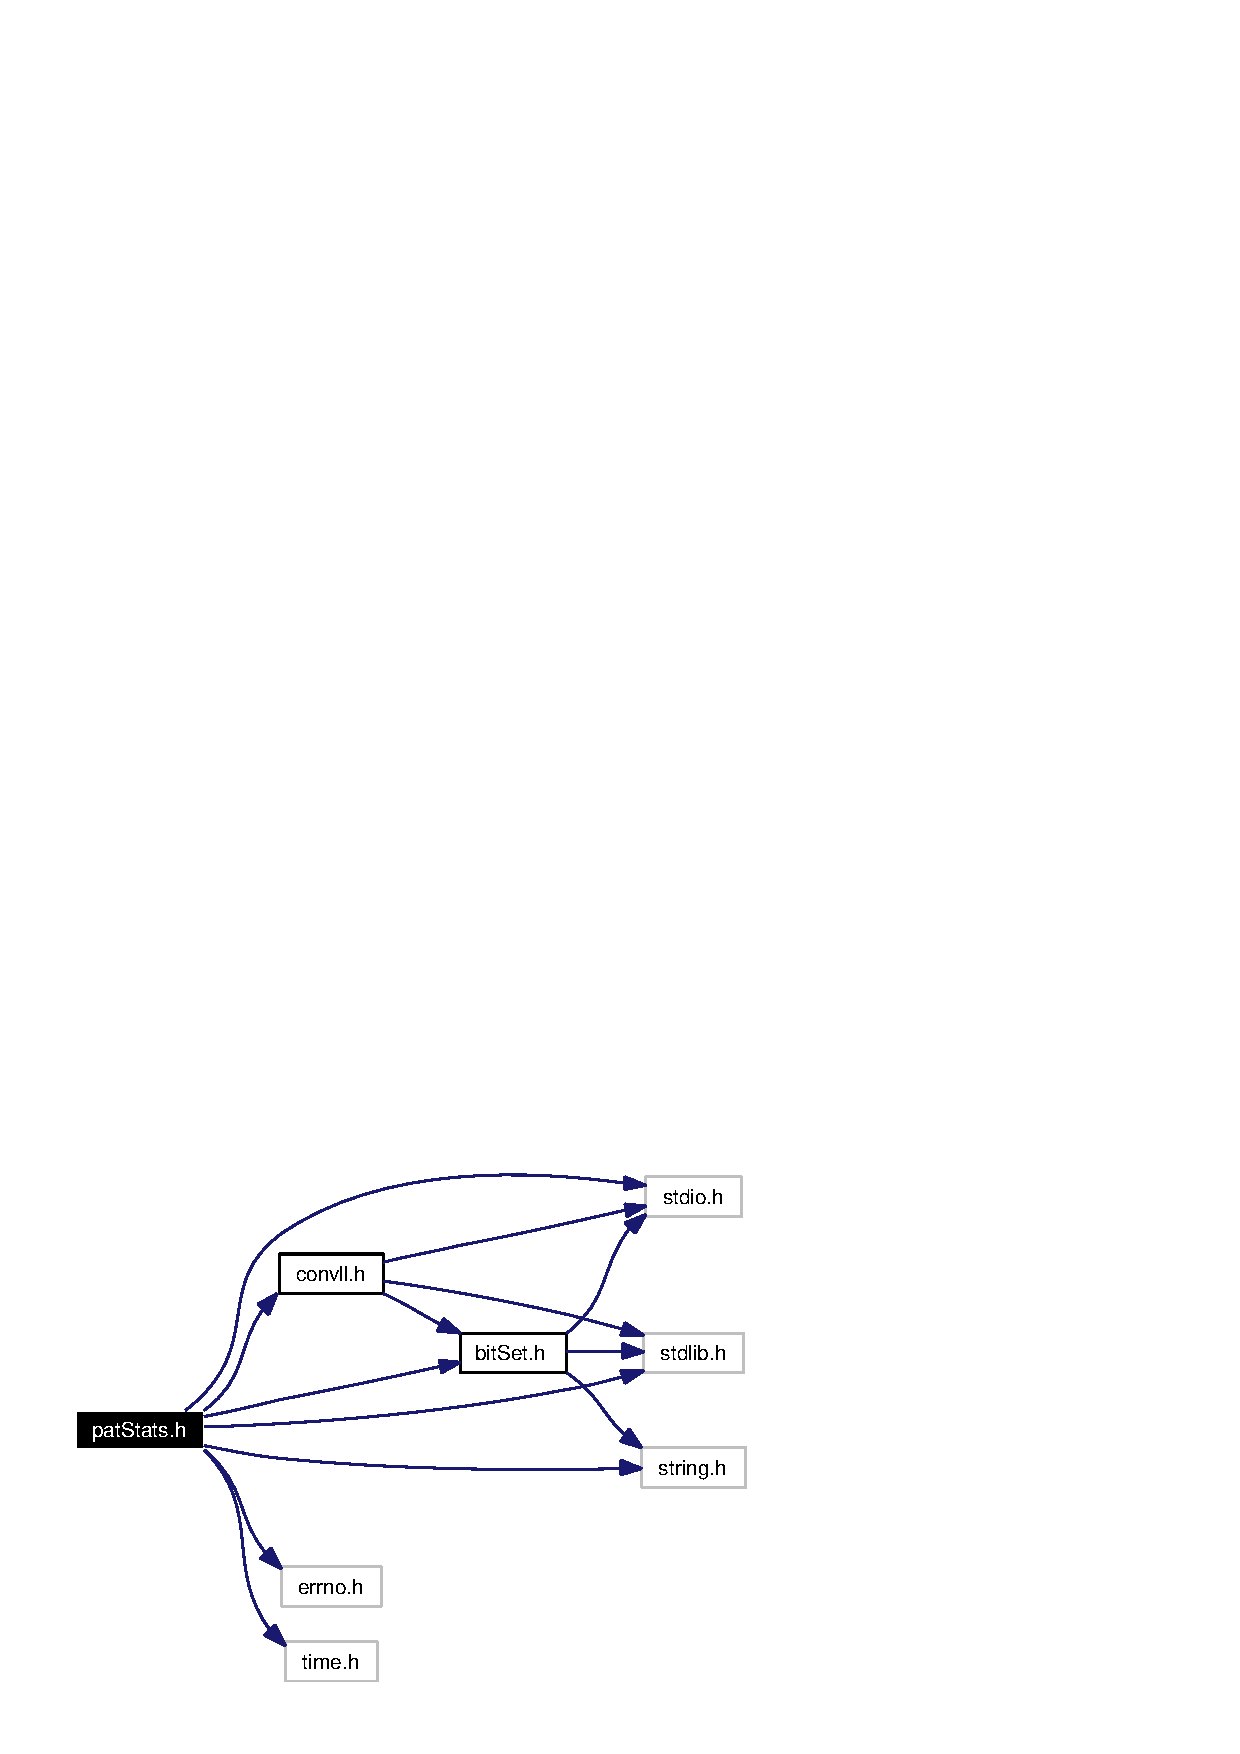
\includegraphics[width=179pt]{patStats_8h__incl}
\end{center}
\end{figure}


This graph shows which files directly or indirectly include this file:\begin{figure}[H]
\begin{center}
\leavevmode
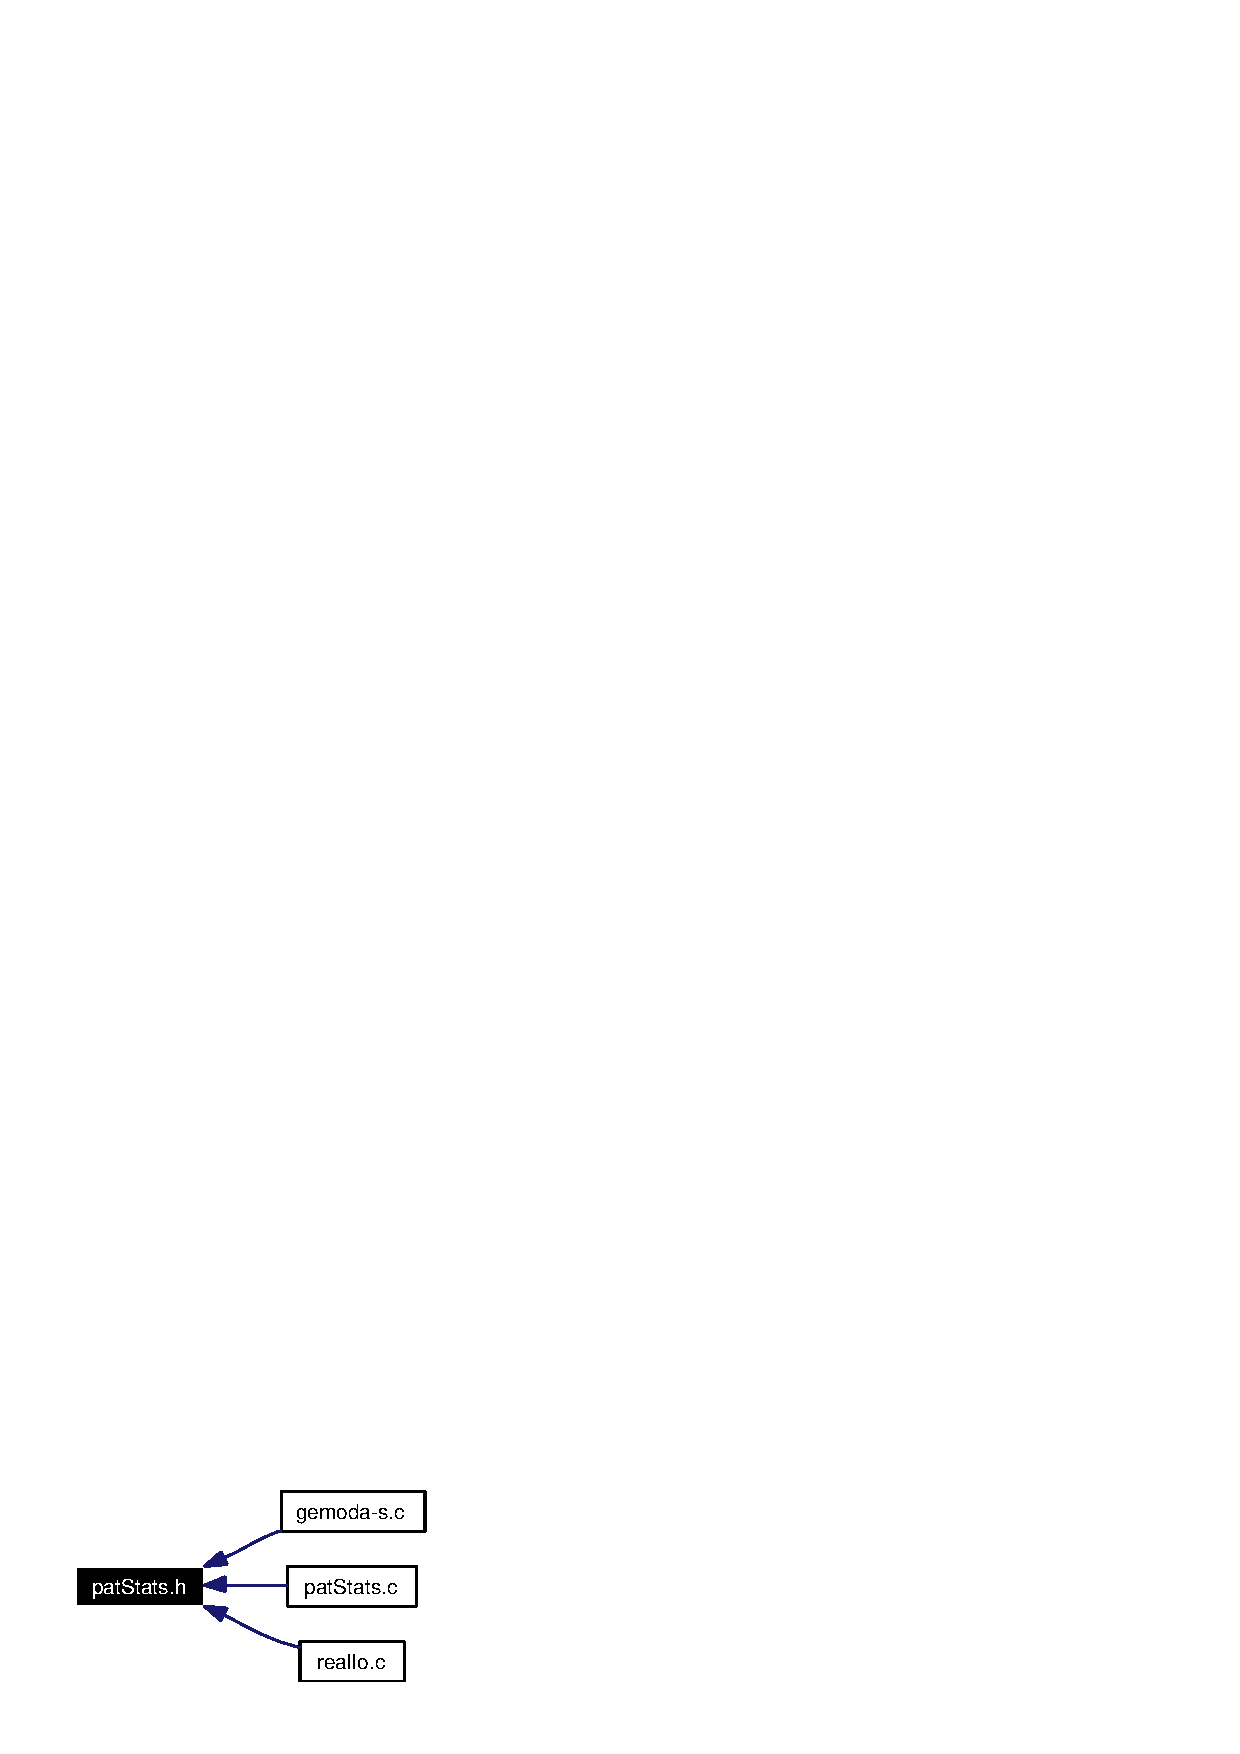
\includegraphics[width=102pt]{patStats_8h__dep__incl}
\end{center}
\end{figure}
\subsection*{Functions}
\begin{CompactItemize}
\item 
unsigned int $\ast$$\ast$ \hyperlink{patStats_8h_a0}{get\-Stat\-Mat} (\hyperlink{structbitGraph__t}{bit\-Graph\_\-t} $\ast$bg, int support, int length, int $\ast$support\-Dim, int $\ast$length\-Dim, int num\-Blanks, int s, FILE $\ast$OUTPUT\_\-FILE)
\item 
int \hyperlink{patStats_8h_a1}{cum\-DMatrix} (unsigned int $\ast$$\ast$d, \hyperlink{structcnode}{cll\_\-t} $\ast$cliqs, int curr\-Support, int curr\-Length, int bg\-Size, int num\-Seqs)
\item 
int \hyperlink{patStats_8h_a2}{calc\-Stat\-All\-Cliqs} (unsigned int $\ast$$\ast$d, \hyperlink{structcnode}{cll\_\-t} $\ast$all\-Cliqs, int num\-Windows)
\item 
\hyperlink{structcnode}{cll\_\-t} $\ast$ \hyperlink{patStats_8h_a3}{sort\-By\-Stats} (\hyperlink{structcnode}{cll\_\-t} $\ast$all\-Cliqs)
\item 
int \hyperlink{patStats_8h_a4}{free\-D} (unsigned int $\ast$$\ast$d, int support\-Dim)
\end{CompactItemize}


\subsection*{Function Documentation}
\hypertarget{patStats_8h_a2}{
\index{patStats.h@{pat\-Stats.h}!calcStatAllCliqs@{calcStatAllCliqs}}
\index{calcStatAllCliqs@{calcStatAllCliqs}!patStats.h@{pat\-Stats.h}}
\subsubsection[calcStatAllCliqs]{\setlength{\rightskip}{0pt plus 5cm}int calc\-Stat\-All\-Cliqs (unsigned int $\ast$$\ast$ {\em d}, \hyperlink{structcnode}{cll\_\-t} $\ast$ {\em all\-Cliqs}, int {\em num\-Windows})}}
\label{patStats_8h_a2}




Definition at line 623 of file pat\-Stats.c.

References calc\-Stat\-Cliq(), cnode::next, and cnode::stat.

Referenced by main().



\hypertarget{patStats_8h_a1}{
\index{patStats.h@{pat\-Stats.h}!cumDMatrix@{cumDMatrix}}
\index{cumDMatrix@{cumDMatrix}!patStats.h@{pat\-Stats.h}}
\subsubsection[cumDMatrix]{\setlength{\rightskip}{0pt plus 5cm}int cum\-DMatrix (unsigned int $\ast$$\ast$ {\em d}, \hyperlink{structcnode}{cll\_\-t} $\ast$ {\em cliqs}, int {\em curr\-Support}, int {\em curr\-Length}, int {\em bg\-Size}, int {\em num\-Seqs})}}
\label{patStats_8h_a1}




Definition at line 460 of file pat\-Stats.c.

References get\-Largest\-Length(), and get\-Largest\-Support().

Referenced by main().



\hypertarget{patStats_8h_a4}{
\index{patStats.h@{pat\-Stats.h}!freeD@{freeD}}
\index{freeD@{freeD}!patStats.h@{pat\-Stats.h}}
\subsubsection[freeD]{\setlength{\rightskip}{0pt plus 5cm}int free\-D (unsigned int $\ast$$\ast$ {\em d}, int {\em support\-Dim})}}
\label{patStats_8h_a4}




Definition at line 637 of file pat\-Stats.c.

Referenced by main().



\hypertarget{patStats_8h_a0}{
\index{patStats.h@{pat\-Stats.h}!getStatMat@{getStatMat}}
\index{getStatMat@{getStatMat}!patStats.h@{pat\-Stats.h}}
\subsubsection[getStatMat]{\setlength{\rightskip}{0pt plus 5cm}unsigned int$\ast$$\ast$ get\-Stat\-Mat (\hyperlink{structbitGraph__t}{bit\-Graph\_\-t} $\ast$ {\em bg}, int {\em support}, int {\em length}, int $\ast$ {\em support\-Dim}, int $\ast$ {\em length\-Dim}, int {\em num\-Blanks}, int {\em s}, FILE $\ast$ {\em OUTPUT\_\-FILE})}}
\label{patStats_8h_a0}




Definition at line 289 of file pat\-Stats.c.

References bit\-Graph\-Row\-Intersection(), check\-Bit(), count\-Set(), delete\-Bit\-Set(), bit\-Graph\_\-t::graph, increase\-Mem(), measure\-Diagonal(), new\-Bit\-Set(), next\-Bit\-Bit\-Set(), and bit\-Graph\_\-t::size.

Referenced by main().



\hypertarget{patStats_8h_a3}{
\index{patStats.h@{pat\-Stats.h}!sortByStats@{sortByStats}}
\index{sortByStats@{sortByStats}!patStats.h@{pat\-Stats.h}}
\subsubsection[sortByStats]{\setlength{\rightskip}{0pt plus 5cm}\hyperlink{structcnode}{cll\_\-t}$\ast$ sort\-By\-Stats (\hyperlink{structcnode}{cll\_\-t} $\ast$ {\em all\-Cliqs})}}
\label{patStats_8h_a3}


This function is used to sort a link to list of cliques by the statistical significance of the motifs found in that linked list.

Definition at line 674 of file pat\-Stats.c.

References cnode::id.

Referenced by main().




\hypertarget{realCompare_8c}{
\section{real\-Compare.c File Reference}
\label{realCompare_8c}\index{realCompare.c@{realCompare.c}}
}
{\tt \#include \char`\"{}real\-Compare.h\char`\"{}}\par


Include dependency graph for real\-Compare.c:\begin{figure}[H]
\begin{center}
\leavevmode
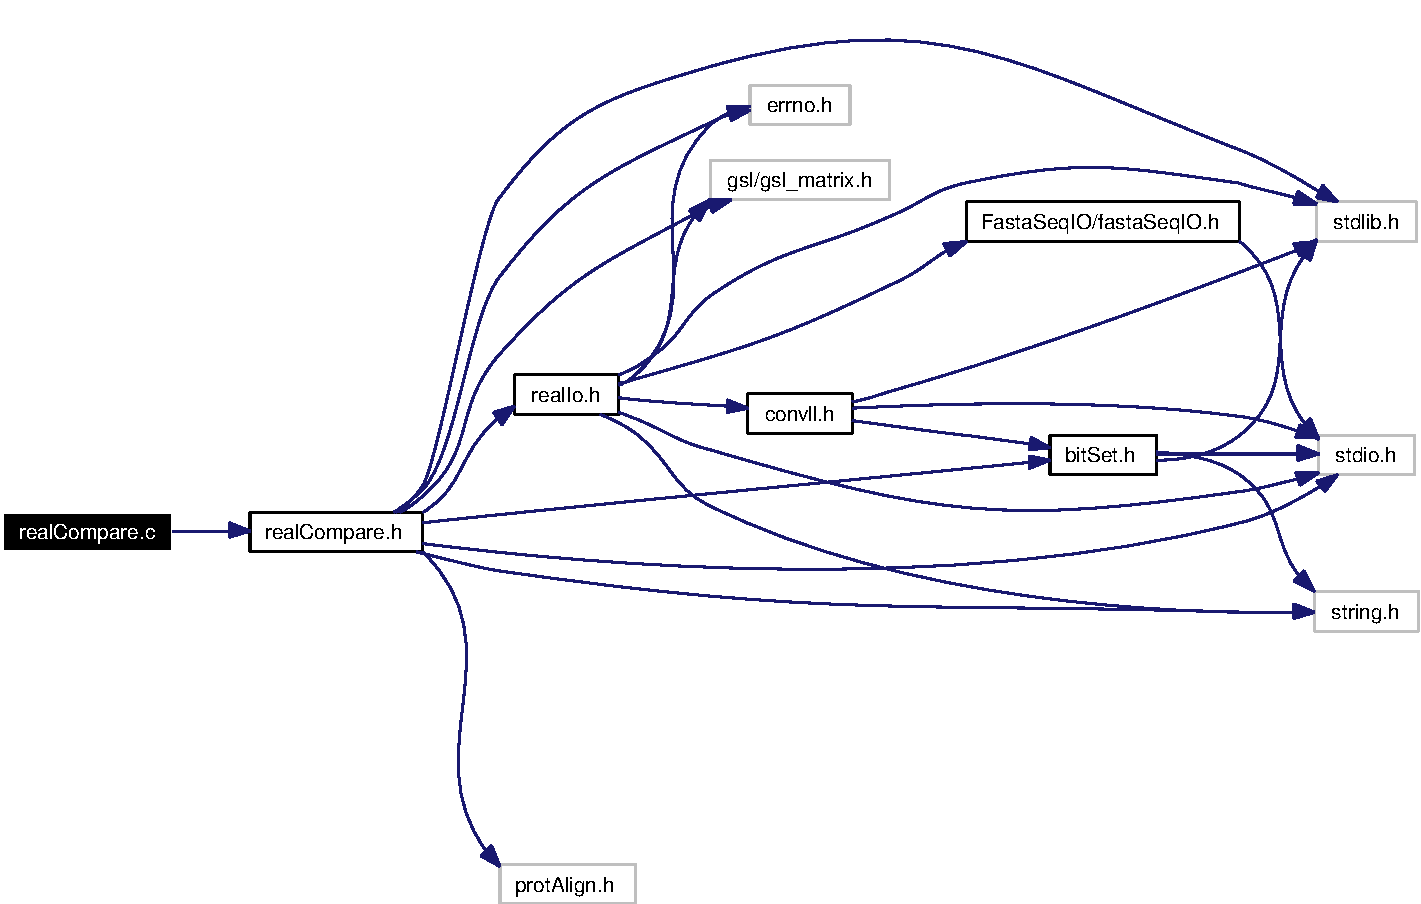
\includegraphics[width=358pt]{realCompare_8c__incl}
\end{center}
\end{figure}
\subsection*{Functions}
\begin{CompactItemize}
\item 
double \hyperlink{realCompare_8c_a0}{rmsd\-Compare} (\hyperlink{structrdh__t}{rdh\_\-t} $\ast$data, int win1, int win2, int L, double $\ast$extra\-Params)
\item 
double \hyperlink{realCompare_8c_a1}{general\-Match\-Factor} (\hyperlink{structrdh__t}{rdh\_\-t} $\ast$data, int win1, int win2, int L, double $\ast$extra\-Params)
\item 
double \hyperlink{realCompare_8c_a2}{mass\-Spec\-Compare\-WElut} (\hyperlink{structrdh__t}{rdh\_\-t} $\ast$data, int win1, int win2, int L, double $\ast$extra\-Params)
\item 
double($\ast$)(\hyperlink{structrdh__t}{rdh\_\-t} $\ast$, int, int, int, double $\ast$) \hyperlink{realCompare_8c_a3}{get\-Comp\-Func} (int comp\-Func)
\item 
\hyperlink{structbitGraph__t}{bit\-Graph\_\-t} $\ast$ \hyperlink{realCompare_8c_a4}{real\-Comparison} (\hyperlink{structrdh__t}{rdh\_\-t} $\ast$data, int L, double g, int comp\-Func, double $\ast$extra\-Params)
\end{CompactItemize}


\subsection*{Detailed Description}
This file defines a series of functions that are used during the comparison phase of the Gemoda algorithm in the real valued implementation. We define a handful of comparison functions --- some that are well suited to protein structure comparison and others that are more suited to the comparison of mass spectrometry spectra.

Definition in file \hyperlink{realCompare_8c-source}{real\-Compare.c}.

\subsection*{Function Documentation}
\hypertarget{realCompare_8c_a1}{
\index{realCompare.c@{real\-Compare.c}!generalMatchFactor@{generalMatchFactor}}
\index{generalMatchFactor@{generalMatchFactor}!realCompare.c@{real\-Compare.c}}
\subsubsection[generalMatchFactor]{\setlength{\rightskip}{0pt plus 5cm}double general\-Match\-Factor (\hyperlink{structrdh__t}{rdh\_\-t} $\ast$ {\em data}, int {\em win1}, int {\em win2}, int {\em L}, double $\ast$ {\em extra\-Params})}}
\label{realCompare_8c_a1}


This function is used to compute a generalized match factor, which is useful for computing the degree of similarity between mass spectrometry spectra.

Definition at line 111 of file real\-Compare.c.

References get\-Rdh\-Dim(), get\-Rdh\-Index\-Seq\-Pos(), and rdh\_\-t::seq.

Referenced by get\-Comp\-Func().

\scriptsize\begin{verbatim}113 {
114   int i, j;
115   double numerator = 0.0;
116   
117     /*
118        double denominator=0.0;
119      */ 
120   double xsum;
121   double ysum;
122   double ldenom = 0.0;
123   double rdenom = 0.0;
124   int dim;
125   int seq1, pos1;
126   int seq2, pos2;
127   gsl_matrix_view view1;
128   gsl_matrix_view view2;
129   gsl_matrix * mat1;
130   gsl_matrix * mat2;
131   dim = getRdhDim (data);
132   
133     // Find out which seq,pos pairs these two
134     // windows correspond to
135     getRdhIndexSeqPos (data, win1, &seq1, &pos1);
136   getRdhIndexSeqPos (data, win2, &seq2, &pos2);
137   
138     // Get a reference to a submatrix.  That is,
139     // 'chop out' the window.
140     view1 = gsl_matrix_submatrix (data->seq[seq1], pos1, 0, L, dim);
141   view2 = gsl_matrix_submatrix (data->seq[seq2], pos2, 0, L, dim);
142   
143     // Some error checking here would be nice!
144     // Did we get the matrices we wanted?
145     
146     // This just makes it easier to handle the views
147     mat1 = &view1.matrix;
148   mat2 = &view2.matrix;
149   
150     // Loop over each position
151     for (i = 0; i < mat1->size1; i++)
152     {
153       xsum = 0.0;
154       ysum = 0.0;
155       
156     // Loop over each dimension at each position
157     for (j = 0; j < dim; j++)
158     {
159       xsum += gsl_matrix_get (mat1, i, j);
160       ysum += gsl_matrix_get (mat2, i, j);
161     }
162       numerator += (i + 1) * sqrt (xsum * ysum);
163       ldenom += (i + 1) * xsum;
164       rdenom += (i + 1) * ysum;
165     }
166   return pow (numerator, 2.0) / (ldenom * rdenom);
167 }
\end{verbatim}
\normalsize 


\hypertarget{realCompare_8c_a3}{
\index{realCompare.c@{real\-Compare.c}!getCompFunc@{getCompFunc}}
\index{getCompFunc@{getCompFunc}!realCompare.c@{real\-Compare.c}}
\subsubsection[getCompFunc]{\setlength{\rightskip}{0pt plus 5cm}double($\ast$)(\hyperlink{structrdh__t}{rdh\_\-t} $\ast$, int, int, int, double $\ast$) get\-Comp\-Func ()}}
\label{realCompare_8c_a3}




Definition at line 264 of file real\-Compare.c.

References general\-Match\-Factor(), mass\-Spec\-Compare\-WElut(), and rmsd\-Compare().

\scriptsize\begin{verbatim}265 {
266   double (*comparisonFunc) (rdh_t *, int, int, int, double *) = &rmsdCompare;
267   switch (compFunc)
268     {
269     case 0:
270       comparisonFunc = &rmsdCompare;
271       break;
272     case 1:
273       comparisonFunc = &generalMatchFactor;
274       break;
275     case 2:
276       comparisonFunc = &massSpecCompareWElut;
277       break;
278     default:
279       comparisonFunc = &rmsdCompare;
280       break;
281     }
282   return (comparisonFunc);
283 }
\end{verbatim}
\normalsize 


\hypertarget{realCompare_8c_a2}{
\index{realCompare.c@{real\-Compare.c}!massSpecCompareWElut@{massSpecCompareWElut}}
\index{massSpecCompareWElut@{massSpecCompareWElut}!realCompare.c@{real\-Compare.c}}
\subsubsection[massSpecCompareWElut]{\setlength{\rightskip}{0pt plus 5cm}double mass\-Spec\-Compare\-WElut (\hyperlink{structrdh__t}{rdh\_\-t} $\ast$ {\em data}, int {\em win1}, int {\em win2}, int {\em L}, double $\ast$ {\em extra\-Params})}}
\label{realCompare_8c_a2}


This function is used to compute the match factor between to mass spectrometry spectra in a similar manner to the previous function; however, this function imposes a penalty for spectra that are separated by large distances in elution time. This function is commonly used by Spec\-Connect.

Definition at line 178 of file real\-Compare.c.

References get\-Rdh\-Dim(), get\-Rdh\-Index\-Seq\-Pos(), and rdh\_\-t::seq.

Referenced by get\-Comp\-Func().

\scriptsize\begin{verbatim}180 {
181   int i, j;
182   double numerator = 0.0;
183   
184     /*
185        double denominator=0.0;
186      */ 
187   double xsum;
188   double ysum;
189   double cum;
190   double ldenom = 0.0;
191   double rdenom = 0.0;
192   int dim;
193   int seq1, pos1;
194   int seq2, pos2;
195   double weight = 2.0;
196   gsl_matrix_view view1;
197   gsl_matrix_view view2;
198   gsl_matrix * mat1;
199   gsl_matrix * mat2;
200   double maxElut = -1;
201   if (extraParams != NULL)
202     {
203       maxElut = extraParams[0];
204     }
205   dim = getRdhDim (data);
206   
207     // Find out which seq,pos pairs these two
208     // windows correspond to
209     getRdhIndexSeqPos (data, win1, &seq1, &pos1);
210   getRdhIndexSeqPos (data, win2, &seq2, &pos2);
211   
212     // Get a reference to a submatrix.  That is,
213     // 'chop out' the window.
214     view1 = gsl_matrix_submatrix (data->seq[seq1], pos1, 0, L, dim);
215   view2 = gsl_matrix_submatrix (data->seq[seq2], pos2, 0, L, dim);
216   
217     // Some error checking here would be nice!
218     // Did we get the matrices we wanted?
219     
220     // This just makes it easier to handle the views
221     mat1 = &view1.matrix;
222   mat2 = &view2.matrix;
223   cum = 1.0;
224   
225     // Loop over each position
226     for (i = 0; i < mat1->size1; i++)
227     {
228       xsum = 0.0;
229       ysum = 0.0;
230       
231     // First take the first dimension for elution time
232     if (maxElut >= 0)
233     {
234       if (fabs
235            (gsl_matrix_get (mat1, i, 0) - gsl_matrix_get (mat2, i, 0)) >
236            maxElut)
237         {
238           cum = 0;
239           break;
240         }
241     }
242       
243     // printf("\n");
244     // 
245     // Loop over each subsequent dimension at each position
246     for (j = 1; j < dim; j++)
247     {
248       
249         // printf("mat1val=%lf,mat2val=%lf\n",gsl_matrix_get(mat1,i,j),
250         // gsl_matrix_get(mat2,i,j));
251         numerator += pow (j, weight) * sqrt (gsl_matrix_get (mat1, i, j) 
252                          *gsl_matrix_get (mat2, i,
253                                   j));
254       ldenom += pow (j, weight) * gsl_matrix_get (mat1, i, j);
255       rdenom += pow (j, weight) * gsl_matrix_get (mat2, i, j);
256       
257         // printf("numer=%lf,ldenom=%lf,rdenom=%lf\n",numerator,
258         // ldenom,rdenom);
259     }
260       cum *= pow (numerator, 2.0) / (ldenom * rdenom);
261     }
262   return pow (cum, 1.0 / L);
263 }
\end{verbatim}
\normalsize 


\hypertarget{realCompare_8c_a4}{
\index{realCompare.c@{real\-Compare.c}!realComparison@{realComparison}}
\index{realComparison@{realComparison}!realCompare.c@{real\-Compare.c}}
\subsubsection[realComparison]{\setlength{\rightskip}{0pt plus 5cm}\hyperlink{structbitGraph__t}{bit\-Graph\_\-t}$\ast$ real\-Comparison (\hyperlink{structrdh__t}{rdh\_\-t} $\ast$ {\em data}, int {\em L}, double {\em g}, int {\em comp\-Func}, double $\ast$ {\em extra\-Params})}}
\label{realCompare_8c_a4}




Definition at line 285 of file real\-Compare.c.

References bit\-Graph\-Set\-True\-Sym(), get\-Comp\-Func, get\-Rdh\-Index\-Seq\-Pos(), rdh\_\-t::index\-Size, init\-Rdh\-Index(), new\-Bit\-Graph(), and rmsd\-Compare().

Referenced by main().

\scriptsize\begin{verbatim}287 {
288   int i, j;
289   int seq1, pos1;
290   int seq2, pos2;
291   bitGraph_t * bg = NULL;
292   double score;
293   double (*comparisonFunc) (rdh_t *, int, int, int, double *) = &rmsdCompare;
294   
295     // Initialize the rdh's index
296     initRdhIndex (data, L, 1);
297   
298     // Allocate a new bit graph
299     bg = newBitGraph (data->indexSize);
300   
301     // Choose the comparison function, pass a reference to it
302     comparisonFunc = getCompFunc (compFunc);
303   for (i = 0; i < data->indexSize; i++)
304     {
305       
306     // Skip seperators
307     getRdhIndexSeqPos (data, i, &seq1, &pos1);
308       if (seq1 == -1 || pos1 == -1)
309     {
310       continue;
311     }
312       for (j = i; j < data->indexSize; j++)
313     {
314       getRdhIndexSeqPos (data, j, &seq2, &pos2);
315       if (seq2 == -1 || pos2 == -1)
316         {
317           continue;
318         }
319       
320         // This is the comparison function
321         score = comparisonFunc (data, i, j, L, extraParams);
322       
323         // printf("score (%2d,%2d) vs. (%2d, %2d) =\t%lf\n",seq1, pos1, seq2, pos2,
324         // score);
325         if (compFunc == 0)
326         {
327           if (score <= g)
328         {
329           bitGraphSetTrueSym (bg, i, j);
330         }
331         }
332       else if ((compFunc == 1) || (compFunc == 2))
333         {
334           if (score >= g)
335         {
336           bitGraphSetTrueSym (bg, i, j);
337         }
338         }
339       else
340         {
341           fprintf (stderr, "Comparison function undefined in " 
342             "realComparison function,\n located in " 
343             "realCompare.c.  Exiting.\n\n");
344           fflush (stderr);
345           exit (0);
346         }
347     }
348     }
349   return bg;
350 }
\end{verbatim}
\normalsize 


\hypertarget{realCompare_8c_a0}{
\index{realCompare.c@{real\-Compare.c}!rmsdCompare@{rmsdCompare}}
\index{rmsdCompare@{rmsdCompare}!realCompare.c@{real\-Compare.c}}
\subsubsection[rmsdCompare]{\setlength{\rightskip}{0pt plus 5cm}double rmsd\-Compare (\hyperlink{structrdh__t}{rdh\_\-t} $\ast$ {\em data}, int {\em win1}, int {\em win2}, int {\em L}, double $\ast$ {\em extra\-Params})}}
\label{realCompare_8c_a0}


Calculate the rmsd between two windows, with optional translation and rotation. The input to this function is a real data handler object, two integers that point to the windows within the real data that are to be compared, an integer that specifies the length of the windows, and a pointer to a double precision floating point that can be used to store other parameters as needed. This last parameter is most useful for implementing other comparison functions, without having to make, too many changes to other parts of the code.

This function operates in three stages. First, we compute the centroid of each window and move the second window such that its centroid overlaps with that of the first window. Second, we use rigid body rotation to find the rotational matrix that minimizes the root mean squared deviation between the two windows. Finally, this function returns that minimized RMSD.

Definition at line 31 of file real\-Compare.c.

References get\-Rdh\-Dim(), get\-Rdh\-Index\-Seq\-Pos(), and rdh\_\-t::seq.

Referenced by get\-Comp\-Func(), and real\-Comparison().

\scriptsize\begin{verbatim}32 {
33   int trans = 1;
34   int rot = 1;
35   int dim;
36   double result = 0;
37   int seq1, pos1;
38   int seq2, pos2;
39   gsl_matrix_view view1;
40   gsl_matrix_view view2;
41   gsl_matrix * mat1;
42   gsl_matrix * mat2;
43   gsl_matrix * mat1copy;
44   gsl_matrix * mat2copy;
45   
46     // The "rint" function is in math.h and rounds a number to the 
47     // nearest integer.  It raises an "inexact exception" if the
48     // number initially wasn't an integer.
49     if (extraParams != NULL)
50     {
51       trans = rint (extraParams[0]);
52       rot = rint (extraParams[1]);
53     }
54   dim = getRdhDim (data);
55   
56     // Find out which seq,pos pairs these two
57     // windows correspond to
58     getRdhIndexSeqPos (data, win1, &seq1, &pos1);
59   getRdhIndexSeqPos (data, win2, &seq2, &pos2);
60   
61     // Get a reference to a submatrix.  That is,
62     // 'chop out' the window.
63     view1 = gsl_matrix_submatrix (data->seq[seq1], pos1, 0, L, dim);
64   view2 = gsl_matrix_submatrix (data->seq[seq2], pos2, 0, L, dim);
65   
66     // This just makes it easier to handle the views
67     mat1 = &view1.matrix;
68   mat2 = &view2.matrix;
69   
70     // Create copies of the windows, because our comparison
71     // will require altering the matrices
72     mat1copy = gsl_matrix_alloc (mat1->size1, mat1->size2);
73   mat2copy = gsl_matrix_alloc (mat2->size1, mat2->size2);
74   gsl_matrix_memcpy (mat1copy, mat1);
75   gsl_matrix_memcpy (mat2copy, mat2);
76   
77     /*
78         printf("matrix1:\n"); gsl_matrix_pretty_fprintf(stdout, mat1copy, "%f ");
79        printf("\nmatrix2:\n"); gsl_matrix_pretty_fprintf(stdout, mat2copy, "%f "); 
80      */ 
81     
82     // Are we going to do a translation?
83     if (trans == 1)
84     {
85       moveToCentroid (mat1copy);
86       moveToCentroid (mat2copy);
87     }
88   
89     // Are we going to do a rotation?
90     if (rot == 1)
91     {
92       
93     // Rotate mat2copy to have a minimal
94     // rmsd with mat1copy
95     rotateMats (mat1copy, mat2copy);
96     }
97   
98     // Compute the rmsd between mat2copy and mat2copy
99     result = gsl_matrix_rmsd (mat1copy, mat2copy);
100   gsl_matrix_free (mat1copy);
101   gsl_matrix_free (mat2copy);
102   return result;
103 }
\end{verbatim}
\normalsize 



\hypertarget{realCompare_8h}{
\section{real\-Compare.h File Reference}
\label{realCompare_8h}\index{realCompare.h@{realCompare.h}}
}
{\tt \#include $<$stdio.h$>$}\par
{\tt \#include $<$stdlib.h$>$}\par
{\tt \#include $<$string.h$>$}\par
{\tt \#include $<$errno.h$>$}\par
{\tt \#include $<$gsl/gsl\_\-matrix.h$>$}\par
{\tt \#include \char`\"{}real\-Io.h\char`\"{}}\par
{\tt \#include \char`\"{}bit\-Set.h\char`\"{}}\par
{\tt \#include \char`\"{}prot\-Align.h\char`\"{}}\par


Include dependency graph for real\-Compare.h:\begin{figure}[H]
\begin{center}
\leavevmode
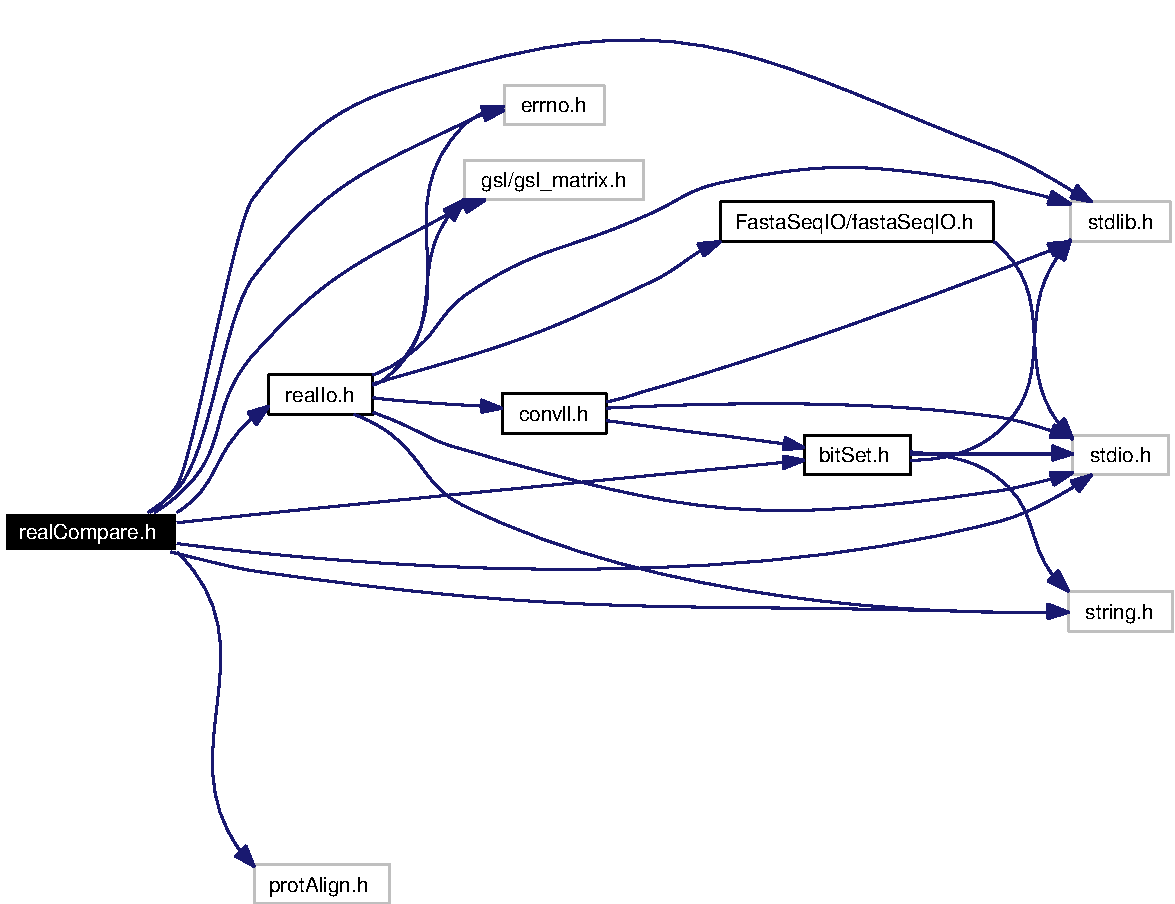
\includegraphics[width=299pt]{realCompare_8h__incl}
\end{center}
\end{figure}


This graph shows which files directly or indirectly include this file:\begin{figure}[H]
\begin{center}
\leavevmode
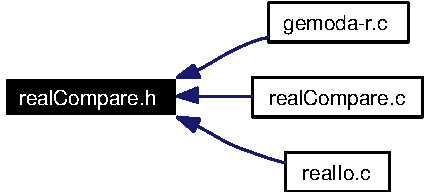
\includegraphics[width=119pt]{realCompare_8h__dep__incl}
\end{center}
\end{figure}
\subsection*{Functions}
\begin{CompactItemize}
\item 
double \hyperlink{realCompare_8h_a1}{rmsd\-Compare} (\hyperlink{structrdh__t}{rdh\_\-t} $\ast$data, int win1, int win2, int L, double $\ast$extra\-Params)
\item 
double \hyperlink{realCompare_8h_a2}{general\-Match\-Factor} (\hyperlink{structrdh__t}{rdh\_\-t} $\ast$data, int win1, int win2, int L, double $\ast$extra\-Params)
\item 
double \hyperlink{realCompare_8h_a3}{mass\-Spec\-Compare\-WElut} (\hyperlink{structrdh__t}{rdh\_\-t} $\ast$data, int win1, int win2, int L, double $\ast$extra\-Params)
\item 
\hyperlink{structbitGraph__t}{bit\-Graph\_\-t} $\ast$ \hyperlink{realCompare_8h_a4}{real\-Comparison} (\hyperlink{structrdh__t}{rdh\_\-t} $\ast$data, int l, double g, int comp\-Func, double $\ast$extra\-Params)
\end{CompactItemize}
\subsection*{Variables}
\begin{CompactItemize}
\item 
double($\ast$)(\hyperlink{structrdh__t}{rdh\_\-t} $\ast$, int, int, int, double $\ast$) \hyperlink{realCompare_8h_a0}{get\-Comp\-Func} (int comp\-Func)
\end{CompactItemize}


\subsection*{Detailed Description}
This file contains declarations and definitions used for the comparison of real valued data during the comparison phase of Gemoda. The functions declared here are defined in \hyperlink{realCompare_8c}{real\-Compare.c}.

Definition in file \hyperlink{realCompare_8h-source}{real\-Compare.h}.

\subsection*{Function Documentation}
\hypertarget{realCompare_8h_a2}{
\index{realCompare.h@{real\-Compare.h}!generalMatchFactor@{generalMatchFactor}}
\index{generalMatchFactor@{generalMatchFactor}!realCompare.h@{real\-Compare.h}}
\subsubsection[generalMatchFactor]{\setlength{\rightskip}{0pt plus 5cm}double general\-Match\-Factor (\hyperlink{structrdh__t}{rdh\_\-t} $\ast$ {\em data}, int {\em win1}, int {\em win2}, int {\em L}, double $\ast$ {\em extra\-Params})}}
\label{realCompare_8h_a2}


This function is used to compute a generalized match factor, which is useful for computing the degree of similarity between mass spectrometry spectra.

Definition at line 111 of file real\-Compare.c.

References get\-Rdh\-Dim(), get\-Rdh\-Index\-Seq\-Pos(), and rdh\_\-t::seq.

Referenced by get\-Comp\-Func().



\hypertarget{realCompare_8h_a3}{
\index{realCompare.h@{real\-Compare.h}!massSpecCompareWElut@{massSpecCompareWElut}}
\index{massSpecCompareWElut@{massSpecCompareWElut}!realCompare.h@{real\-Compare.h}}
\subsubsection[massSpecCompareWElut]{\setlength{\rightskip}{0pt plus 5cm}double mass\-Spec\-Compare\-WElut (\hyperlink{structrdh__t}{rdh\_\-t} $\ast$ {\em data}, int {\em win1}, int {\em win2}, int {\em L}, double $\ast$ {\em extra\-Params})}}
\label{realCompare_8h_a3}


This function is used to compute the match factor between to mass spectrometry spectra in a similar manner to the previous function; however, this function imposes a penalty for spectra that are separated by large distances in elution time. This function is commonly used by Spec\-Connect.

Definition at line 174 of file real\-Compare.c.

References get\-Rdh\-Dim(), get\-Rdh\-Index\-Seq\-Pos(), and rdh\_\-t::seq.

Referenced by get\-Comp\-Func().



\hypertarget{realCompare_8h_a4}{
\index{realCompare.h@{real\-Compare.h}!realComparison@{realComparison}}
\index{realComparison@{realComparison}!realCompare.h@{real\-Compare.h}}
\subsubsection[realComparison]{\setlength{\rightskip}{0pt plus 5cm}\hyperlink{structbitGraph__t}{bit\-Graph\_\-t}$\ast$ real\-Comparison (\hyperlink{structrdh__t}{rdh\_\-t} $\ast$ {\em data}, int {\em l}, double {\em g}, int {\em comp\-Func}, double $\ast$ {\em extra\-Params})}}
\label{realCompare_8h_a4}




Definition at line 272 of file real\-Compare.c.

References bit\-Graph\-Set\-True\-Sym(), get\-Comp\-Func, get\-Rdh\-Index\-Seq\-Pos(), rdh\_\-t::index\-Size, init\-Rdh\-Index(), new\-Bit\-Graph(), and rmsd\-Compare().

Referenced by main().



\hypertarget{realCompare_8h_a1}{
\index{realCompare.h@{real\-Compare.h}!rmsdCompare@{rmsdCompare}}
\index{rmsdCompare@{rmsdCompare}!realCompare.h@{real\-Compare.h}}
\subsubsection[rmsdCompare]{\setlength{\rightskip}{0pt plus 5cm}double rmsd\-Compare (\hyperlink{structrdh__t}{rdh\_\-t} $\ast$ {\em data}, int {\em win1}, int {\em win2}, int {\em L}, double $\ast$ {\em extra\-Params})}}
\label{realCompare_8h_a1}


Calculate the rmsd between two windows, with optional translation and rotation. The input to this function is a real data handler object, two integers that point to the windows within the real data that are to be compared, an integer that specifies the length of the windows, and a pointer to a double precision floating point that can be used to store other parameters as needed. This last parameter is most useful for implementing other comparison functions, without having to make, too many changes to other parts of the code.

This function operates in three stages. First, we compute the centroid of each window and move the second window such that its centroid overlaps with that of the first window. Second, we use rigid body rotation to find the rotational matrix that minimizes the root mean squared deviation between the two windows. Finally, this function returns that minimized RMSD.

Definition at line 31 of file real\-Compare.c.

References get\-Rdh\-Dim(), get\-Rdh\-Index\-Seq\-Pos(), and rdh\_\-t::seq.

Referenced by get\-Comp\-Func(), and real\-Comparison().





\subsection*{Variable Documentation}
\hypertarget{realCompare_8h_a0}{
\index{realCompare.h@{real\-Compare.h}!getCompFunc@{getCompFunc}}
\index{getCompFunc@{getCompFunc}!realCompare.h@{real\-Compare.h}}
\subsubsection[getCompFunc]{\setlength{\rightskip}{0pt plus 5cm}double($\ast$)(\hyperlink{structrdh__t}{rdh\_\-t}$\ast$, int, int, int, double$\ast$) get\-Comp\-Func(int comp\-Func)}}
\label{realCompare_8h_a0}




Definition at line 36 of file real\-Compare.h.

Referenced by find\-Clique\-Centroid(), output\-Real\-Pats\-WCentroid(), and real\-Comparison().

\hypertarget{realIo_8c}{
\section{real\-Io.c File Reference}
\label{realIo_8c}\index{realIo.c@{realIo.c}}
}
{\tt \#include \char`\"{}real\-Io.h\char`\"{}}\par
{\tt \#include \char`\"{}real\-Compare.h\char`\"{}}\par
{\tt \#include \char`\"{}pat\-Stats.h\char`\"{}}\par


Include dependency graph for real\-Io.c:\begin{figure}[H]
\begin{center}
\leavevmode
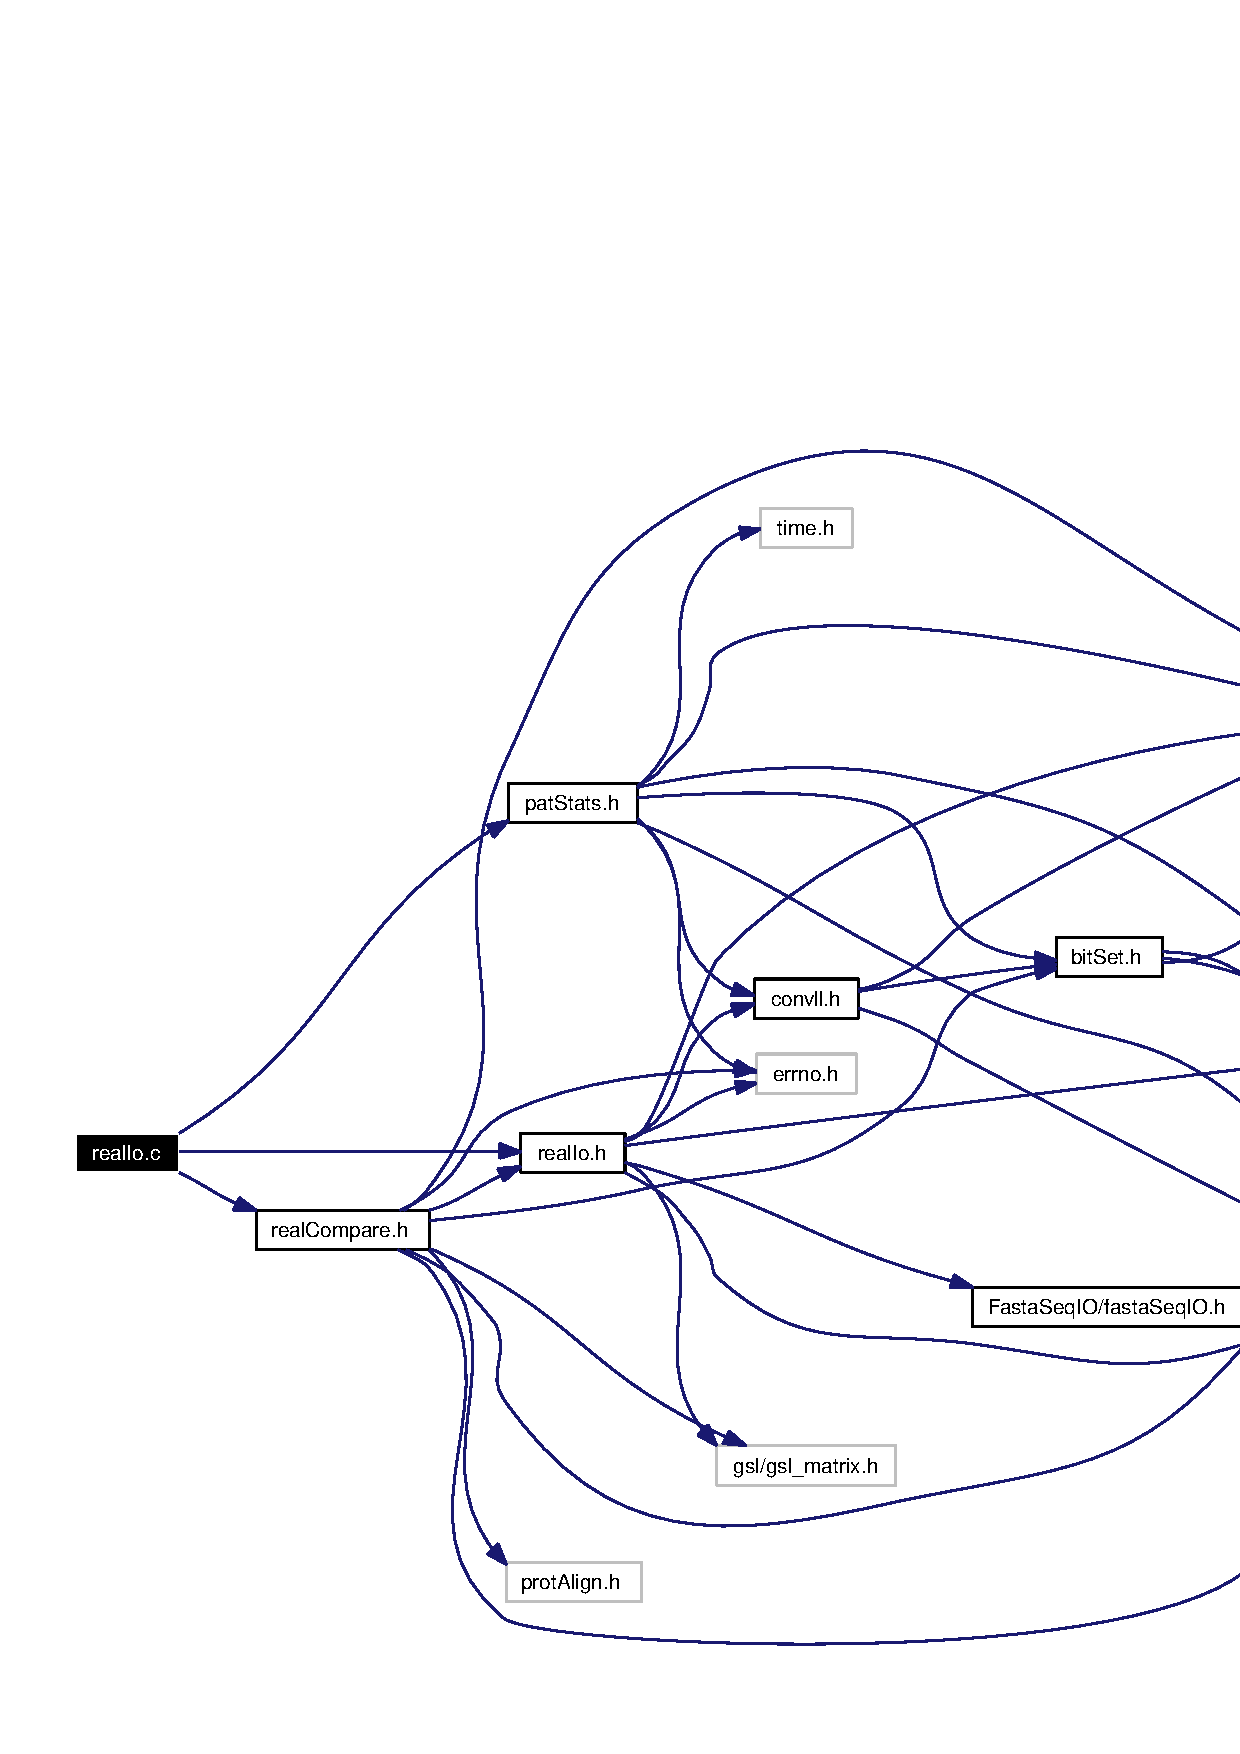
\includegraphics[width=342pt]{realIo_8c__incl}
\end{center}
\end{figure}
\subsection*{Functions}
\begin{CompactItemize}
\item 
\hyperlink{realIo_8c_a0}{word\-To\-Double} (char $\ast$s, int begin, int end)
\item 
int \hyperlink{realIo_8c_a1}{count\-Fields} (char $\ast$s, char sep)
\item 
int \hyperlink{realIo_8c_a2}{check\-Real\-Data\-Format} (char $\ast$$\ast$buf, int nl, char sep, int $\ast$num\-Seq\_\-p, int $\ast$dim\_\-p)
\item 
int \hyperlink{realIo_8c_a3}{count\-Total\-Fields} (char $\ast$$\ast$buf, int nl, char sep)
\item 
\hyperlink{structrdh__t}{rdh\_\-t} $\ast$ \hyperlink{realIo_8c_a4}{init\-Rdh} (int x)
\item 
int \hyperlink{realIo_8c_a5}{get\-Rdh\-Seq\-Length} (\hyperlink{structrdh__t}{rdh\_\-t} $\ast$data, int seq\-No)
\item 
int \hyperlink{realIo_8c_a6}{init\-Rdh\-Index} (\hyperlink{structrdh__t}{rdh\_\-t} $\ast$data, int word\-Size, int seq\-Gap)
\item 
\hyperlink{structrdh__t}{rdh\_\-t} $\ast$ \hyperlink{realIo_8c_a7}{free\-Rdh} (\hyperlink{structrdh__t}{rdh\_\-t} $\ast$data)
\item 
int \hyperlink{realIo_8c_a8}{get\-Rdh\-Dim} (\hyperlink{structrdh__t}{rdh\_\-t} $\ast$data)
\item 
int \hyperlink{realIo_8c_a9}{set\-Rdh\-Label} (\hyperlink{structrdh__t}{rdh\_\-t} $\ast$data, int seq\-No, char $\ast$s)
\item 
int \hyperlink{realIo_8c_a10}{set\-Rdh\-Value} (\hyperlink{structrdh__t}{rdh\_\-t} $\ast$data, int seq\-No, int pos\-No, int dim\-No, double val)
\item 
int \hyperlink{realIo_8c_a11}{set\-Rdh\-Index} (\hyperlink{structrdh__t}{rdh\_\-t} $\ast$data, int seq\-No, int pos\-No, int index)
\item 
int \hyperlink{realIo_8c_a12}{get\-Rdh\-Index\-Seq\-Pos} (\hyperlink{structrdh__t}{rdh\_\-t} $\ast$data, int index, int $\ast$seq, int $\ast$pos)
\item 
double \hyperlink{realIo_8c_a13}{get\-Rdh\-Value} (\hyperlink{structrdh__t}{rdh\_\-t} $\ast$data, int seq\-No, int pos\-No, int dim\-No)
\item 
char $\ast$ \hyperlink{realIo_8c_a14}{get\-Rdh\-Label} (\hyperlink{structrdh__t}{rdh\_\-t} $\ast$data, int seq\-No)
\item 
int \hyperlink{realIo_8c_a15}{print\-Rdh\-Seq} (\hyperlink{structrdh__t}{rdh\_\-t} $\ast$data, int seq\-No, FILE $\ast$FH)
\item 
int \hyperlink{realIo_8c_a16}{set\-Rdh\-Col\-From\-String} (\hyperlink{structrdh__t}{rdh\_\-t} $\ast$data, int seq\-No, int col\-No, char $\ast$s, char sep)
\item 
int \hyperlink{realIo_8c_a17}{init\-Rdh\-Gsl\-Mat} (\hyperlink{structrdh__t}{rdh\_\-t} $\ast$data, int seq\-No, int x, int y)
\item 
int \hyperlink{realIo_8c_a18}{push\-On\-Rdh\-Seq} (\hyperlink{structrdh__t}{rdh\_\-t} $\ast$data, char $\ast$$\ast$buf, int start\-Line, int dim, char sep)
\item 
\hyperlink{structrdh__t}{rdh\_\-t} $\ast$ \hyperlink{realIo_8c_a19}{parse\-Real\-Data} (char $\ast$$\ast$buf, int nl, char sep, int num\-Seq, int dim)
\item 
\hyperlink{structrdh__t}{rdh\_\-t} $\ast$ \hyperlink{realIo_8c_a20}{read\-Real\-Data} (FILE $\ast$INPUT)
\item 
int \hyperlink{realIo_8c_a21}{output\-Real\-Pats} (\hyperlink{structrdh__t}{rdh\_\-t} $\ast$data, \hyperlink{structcnode}{cll\_\-t} $\ast$all\-Pats, int L, FILE $\ast$OUTPUT\_\-FILE, int $\ast$$\ast$d)
\item 
int \hyperlink{realIo_8c_a22}{find\-Clique\-Centroid} (\hyperlink{structrdh__t}{rdh\_\-t} $\ast$data, \hyperlink{structcnode}{cll\_\-t} $\ast$cur\-Cliq, int L, int comp\-Func, double $\ast$extra\-Params, int $\ast$candidates)
\item 
int \hyperlink{realIo_8c_a23}{make\-Alternate\-Centroid} (\hyperlink{structrdh__t}{rdh\_\-t} $\ast$data, \hyperlink{structcnode}{cll\_\-t} $\ast$cur\-Cliq, int $\ast$candidates)
\item 
int \hyperlink{realIo_8c_a24}{output\-Real\-Pats\-WCentroid} (\hyperlink{structrdh__t}{rdh\_\-t} $\ast$data, \hyperlink{structcnode}{cll\_\-t} $\ast$all\-Pats, int L, FILE $\ast$OUTPUT\_\-FILE, double $\ast$extra\-Params, int comp\-Func)
\end{CompactItemize}


\subsection*{Detailed Description}
This file defines functions that are used for the parsing of user supplied data in the real valued implementation of Gemoda.

Definition in file \hyperlink{realIo_8c-source}{real\-Io.c}.

\subsection*{Function Documentation}
\hypertarget{realIo_8c_a2}{
\index{realIo.c@{real\-Io.c}!checkRealDataFormat@{checkRealDataFormat}}
\index{checkRealDataFormat@{checkRealDataFormat}!realIo.c@{real\-Io.c}}
\subsubsection[checkRealDataFormat]{\setlength{\rightskip}{0pt plus 5cm}int check\-Real\-Data\-Format (char $\ast$$\ast$ {\em buf}, int {\em nl}, char {\em sep}, int $\ast$ {\em num\-Seq\_\-p}, int $\ast$ {\em dim\_\-p})}}
\label{realIo_8c_a2}


Check that each sequence has the same dimensionality and that, within a sequence, each dimension has the same number of entries. Note: this routine alters $\ast$nun\-Seq\_\-p and $\ast$dim\_\-p! Also, you must call this routine before calling parse\-Real\-Data. Otherwise, parse\-Real\-Data is garunteed to die if the data turn out to be ill-formatted.

Definition at line 163 of file real\-Io.c.

References count\-Fields().

Referenced by read\-Real\-Data().

\scriptsize\begin{verbatim}164 {
165   int i;
166   int thisDim = 0;
167   int status = 1;
168   int width;
169   int fieldCount = 0;       // number of positions in a single sequence
170   int numSeq = 0;       // number of sequences 
171   int dim = 0;          // The dimensionality of the sequences
172 
173   // NOTE this is not checking the dimensionality of the last sequence...
174   // that's bad.  We can fix that though.
175   // Check the dimensionality of each sequence
176   for (i = 0; i < nl; i++)
177     {
178       if (buf[i][0] == '>')
179     {
180 
181       // If this is only the second sequence we've seen,
182       // record the dimensionality of the first sequence
183       // as the dim to insist upon from here on out
184       if (numSeq == 1)
185         {
186           dim = thisDim;
187 
188           // For other sequences, we need to check to make sure
189           // that they've got the same dimensions as previous
190           // sequences
191         }
192       else if (numSeq > 1)
193         {
194 
195           // If the dimensions are wrong, quit with status=0
196           if (thisDim != dim)
197         {
198           status = 0;
199           break;
200         }
201         }
202       numSeq++;
203       width = 0;
204       thisDim = 0;
205     }
206       else
207     {
208 
209       // Field count can be different for each sequence but
210       // must be the same for each dimension in a single sequence
211       fieldCount = countFields (buf[i], sep);
212 
213       // If this is the first row of this sequence,
214       // then store the number of fields
215       if (thisDim == 0)
216         {
217           width = fieldCount;
218 
219           // If it's not the first row, make sure it has the
220           // same number of fields as previous rows in this
221           // sequence
222         }
223       else
224         {
225           if (fieldCount != width)
226         {
227           status = 0;
228           break;
229         }
230         }
231       thisDim++;
232     }
233     }
234 
235   // Pass back the numSeq and dim
236   *numSeq_p = numSeq;
237   *dim_p = thisDim;
238   return status;
239 }
\end{verbatim}
\normalsize 


\hypertarget{realIo_8c_a1}{
\index{realIo.c@{real\-Io.c}!countFields@{countFields}}
\index{countFields@{countFields}!realIo.c@{real\-Io.c}}
\subsubsection[countFields]{\setlength{\rightskip}{0pt plus 5cm}int count\-Fields (char $\ast$ {\em s}, char {\em sep})}}
\label{realIo_8c_a1}


Count the number of fields (delimited by 'sep') in a single string. I was going to use strsep in string.h for this; however, I don't like that it changes the input string, which makes free-ing the string later more tricky. Ignores consecutive seperators.

Definition at line 90 of file real\-Io.c.

References word\-To\-Double().

Referenced by check\-Real\-Data\-Format(), count\-Total\-Fields(), and push\-On\-Rdh\-Seq().

\scriptsize\begin{verbatim}91 {
92   int i;
93   int begin = 0;
94   int end = 0;
95   int status = 0;       // 0 = in sep, 1 = in word
96   int fieldCount = 0;
97   double val;
98   if (s == NULL)
99     {
100       fprintf (stderr, "Passed NULL string to countFields -- error!");
101       fflush (stderr);
102       exit (0);
103     }
104 
105   // Loop over the length of the string
106   for (i = 0; i < strlen (s); i++)
107     {
108 
109       // The previous state was space
110       if (status == 0)
111     {
112 
113       // We hit a word
114       if (s[i] != sep)
115         {
116           begin = i;
117           status = 1;
118         }
119       else
120         {           // We hit more space
121           continue;
122         }
123     }
124       else
125     {           // The previous state was word
126       if (s[i] != sep)
127         {
128           continue;
129         }
130       else
131         {           // We hit a space
132           end = i - 1;
133           status = 0;
134 
135           // being and end now delimit a word,
136           // turn that word into a double
137           val = wordToDouble (s, begin, end);
138           fieldCount++;
139         }
140     }
141     }
142 
143   // At the end, if we were in a word, we have
144   // one more field
145   if (status == 1)
146     {               // We're in a word
147       val = wordToDouble (s, begin, strlen (s));
148       fieldCount++;
149     }
150   return fieldCount;
151 }
\end{verbatim}
\normalsize 


\hypertarget{realIo_8c_a3}{
\index{realIo.c@{real\-Io.c}!countTotalFields@{countTotalFields}}
\index{countTotalFields@{countTotalFields}!realIo.c@{real\-Io.c}}
\subsubsection[countTotalFields]{\setlength{\rightskip}{0pt plus 5cm}int count\-Total\-Fields (char $\ast$$\ast$ {\em buf}, int {\em nl}, char {\em sep})}}
\label{realIo_8c_a3}


Count the number of fields in each sequence and return the sum of these.

Definition at line 246 of file real\-Io.c.

References count\-Fields().

Referenced by parse\-Real\-Data().

\scriptsize\begin{verbatim}247 {
248   int i = 0;
249   int totalFields = 0;
250   int seqNo = 0;
251   while (i < nl)
252     {
253 
254       // Hit a new sequence
255       if (buf[i][0] == '>')
256     {
257       seqNo++;
258 
259       // Assume that the sequence has at least
260       // one row (should have called checkRealDataFormat!
261       // and that each row has the same number of fields
262       totalFields += countFields (buf[i + 1], sep);
263     }
264       i++;
265     }
266   return totalFields;
267 }
\end{verbatim}
\normalsize 


\hypertarget{realIo_8c_a22}{
\index{realIo.c@{real\-Io.c}!findCliqueCentroid@{findCliqueCentroid}}
\index{findCliqueCentroid@{findCliqueCentroid}!realIo.c@{real\-Io.c}}
\subsubsection[findCliqueCentroid]{\setlength{\rightskip}{0pt plus 5cm}int find\-Clique\-Centroid (\hyperlink{structrdh__t}{rdh\_\-t} $\ast$ {\em data}, \hyperlink{structcnode}{cll\_\-t} $\ast$ {\em cur\-Cliq}, int {\em L}, int {\em comp\-Func}, double $\ast$ {\em extra\-Params}, int $\ast$ {\em candidates})}}
\label{realIo_8c_a22}


This function is used to find the centroid of a clique. That is, to find the center of mass.

Definition at line 1096 of file real\-Io.c.

References get\-Comp\-Func, c\-Set\_\-t::members, cnode::set, and c\-Set\_\-t::size.

Referenced by output\-Real\-Pats\-WCentroid().

\scriptsize\begin{verbatim}1098 {
1099   double (*comparisonFunc) (rdh_t *, int, int, int, double *) = NULL;
1100   int i = 0, j = 0, indmin = -1, counter = 0;
1101   double sim = 0, min = 0, flagmin = 0;
1102   double *cliqueAdjMat = NULL;
1103   cliqueAdjMat = (double *) malloc (curCliq->set->size * sizeof (double));
1104   if (cliqueAdjMat == NULL)
1105     {
1106       fprintf (stderr, "\nMemory Error\n%s\n", strerror (errno));
1107       fflush (stderr);
1108       exit (0);
1109     }
1110   for (i = 0; i < curCliq->set->size; i++)
1111     {
1112       cliqueAdjMat[i] = 0;
1113     }
1114 
1115   // We'll accumulate our comparison function values... except here
1116   // we're really assuming that we're using a match factor, with
1117   // value less than one, so that we can subtract it from one to
1118   // get a distance, and then find the centroid by identifying the
1119   // node with the smallest cumulative Euclidean distance to all
1120   // nodes.  
1121   // Note that we only need to compare each unique pair, and can apply
1122   // the results from each comparison to each member of the pair,
1123   // hence the somewhat odd indices of initiation for the for loops.
1124   comparisonFunc = getCompFunc (compFunc);
1125   for (i = 0; i < curCliq->set->size; i++)
1126     {
1127       for (j = i + 1; j < curCliq->set->size; j++)
1128     {
1129       sim =
1130         comparisonFunc (data, curCliq->set->members[i],
1131                 curCliq->set->members[j], L, extraParams);
1132 
1133       // printf("i = %d, j = %d, L = %d, extra = %lf, sim =
1134       // %lf\n",i,j,L,extraParams[0],sim);
1135       cliqueAdjMat[i] += pow (1 - sim, 2);
1136       cliqueAdjMat[j] += pow (1 - sim, 2);
1137     }
1138     }
1139 
1140   // Now we find the minimum Euclidean distance.
1141   min = cliqueAdjMat[0];
1142   indmin = 0;
1143   for (i = 1; i < curCliq->set->size; i++)
1144     {
1145 
1146       // printf("index %d product = %lf\n",i,cliqueAdjMat[i]);
1147       if (cliqueAdjMat[i] < min)
1148     {
1149       indmin = i;
1150       min = cliqueAdjMat[i];
1151       flagmin = 0;
1152     }
1153       else if (cliqueAdjMat[i] == min)
1154     {
1155       flagmin = 1;
1156     }
1157     }
1158 
1159   // If we had a duplicate on the minimum, we locate all duplicates.
1160   if (flagmin == 1)
1161     {
1162       counter = 0;
1163       for (i = 0; i < curCliq->set->size; i++)
1164     {
1165       if (cliqueAdjMat[i] == min)
1166         {
1167           counter++;
1168           candidates[counter] = i;
1169         }
1170     }
1171 
1172       // Store the number of candidates at the array's beginning
1173       candidates[0] = counter;
1174       free (cliqueAdjMat);
1175       return (-1);
1176     }
1177   else
1178     {
1179       free (cliqueAdjMat);
1180       return (indmin);
1181     }
1182 }
\end{verbatim}
\normalsize 


\hypertarget{realIo_8c_a7}{
\index{realIo.c@{real\-Io.c}!freeRdh@{freeRdh}}
\index{freeRdh@{freeRdh}!realIo.c@{real\-Io.c}}
\subsubsection[freeRdh]{\setlength{\rightskip}{0pt plus 5cm}\hyperlink{structrdh__t}{rdh\_\-t}$\ast$ free\-Rdh (\hyperlink{structrdh__t}{rdh\_\-t} $\ast$ {\em data})}}
\label{realIo_8c_a7}


This function returns a null pointer after freeing the memory associated with a real data holder object. The function takes one parameter: a pointer to the real data holder, {\em data\/}.

Definition at line 462 of file real\-Io.c.

References rdh\_\-t::index\-To\-Pos, rdh\_\-t::index\-To\-Seq, rdh\_\-t::label, rdh\_\-t::offset\-To\-Index, and rdh\_\-t::seq.

Referenced by main().

\scriptsize\begin{verbatim}463 {
464   int i;
465   if (data != NULL)
466     {
467       if (data->indexToPos != NULL)
468     {
469       free (data->indexToPos);
470       data->indexToPos = NULL;
471     }
472       if (data->indexToSeq != NULL)
473     {
474       free (data->indexToSeq);
475       data->indexToSeq = NULL;
476     }
477       if (data->offsetToIndex != NULL)
478     {
479       for (i = 0; i < data->size; i++)
480         {
481           free (data->offsetToIndex[i]);
482           data->offsetToIndex[i] = NULL;
483         }
484       free (data->offsetToIndex);
485       data->offsetToIndex = NULL;
486     }
487       for (i = 0; i < data->size; i++)
488     {
489       if (data->seq[i] != NULL)
490         {
491           gsl_matrix_free (data->seq[i]);
492           data->seq[i] = NULL;
493         }
494       if (data->label[i] != NULL)
495         {
496           free (data->label[i]);
497           data->label[i] = NULL;
498         }
499     }
500       if (data->seq != NULL)
501     {
502       free (data->seq);
503       data->seq = NULL;
504     }
505       if (data->label != NULL)
506     {
507       free (data->label);
508       data->label = NULL;
509     }
510       free (data);
511       data = NULL;
512     }
513   return data;
514 }
\end{verbatim}
\normalsize 


\hypertarget{realIo_8c_a8}{
\index{realIo.c@{real\-Io.c}!getRdhDim@{getRdhDim}}
\index{getRdhDim@{getRdhDim}!realIo.c@{real\-Io.c}}
\subsubsection[getRdhDim]{\setlength{\rightskip}{0pt plus 5cm}int get\-Rdh\-Dim (\hyperlink{structrdh__t}{rdh\_\-t} $\ast$ {\em data})}}
\label{realIo_8c_a8}


This function returns an integer equal to the dimensions of the data stored in a real data holder object. The function takes one parameter: a pointer to the real data holder, {\em data\/}.

Definition at line 524 of file real\-Io.c.

References rdh\_\-t::seq.

Referenced by general\-Match\-Factor(), get\-Rdh\-Value(), mass\-Spec\-Compare\-WElut(), print\-Rdh\-Seq(), rmsd\-Compare(), and set\-Rdh\-Value().

\scriptsize\begin{verbatim}525 {
526   if (data == NULL || data->seq == NULL || data->seq[0] == NULL)
527     {
528       fprintf (stderr, "Passed bad data to getRdhSeqLength -- error!");
529       fflush (stderr);
530       exit (0);
531     }
532   return data->seq[0]->size2;
533 }
\end{verbatim}
\normalsize 


\hypertarget{realIo_8c_a12}{
\index{realIo.c@{real\-Io.c}!getRdhIndexSeqPos@{getRdhIndexSeqPos}}
\index{getRdhIndexSeqPos@{getRdhIndexSeqPos}!realIo.c@{real\-Io.c}}
\subsubsection[getRdhIndexSeqPos]{\setlength{\rightskip}{0pt plus 5cm}int get\-Rdh\-Index\-Seq\-Pos (\hyperlink{structrdh__t}{rdh\_\-t} $\ast$ {\em data}, int {\em index}, int $\ast$ {\em seq}, int $\ast$ {\em pos})}}
\label{realIo_8c_a12}


This function is used to access and change the sequence and position values, given an index. The function takes four parameters: a pointer to the real data holder, {\em data\/}, an integer {\em index\/}, a pointer integer {\em seq\/}, and a pointer integer {\em pos\/}.

Definition at line 633 of file real\-Io.c.

References rdh\_\-t::index\-Size, rdh\_\-t::index\-To\-Pos, and rdh\_\-t::index\-To\-Seq.

Referenced by general\-Match\-Factor(), make\-Alternate\-Centroid(), mass\-Spec\-Compare\-WElut(), output\-Real\-Pats(), output\-Real\-Pats\-WCentroid(), real\-Comparison(), and rmsd\-Compare().

\scriptsize\begin{verbatim}634 {
635   if (data == NULL || data->indexToSeq == NULL || data->indexToPos == NULL
636       || index > data->indexSize)
637     {
638       fprintf (stderr, "Passed bad data to getRdhIndexSeqPos -- error!");
639       fflush (stderr);
640       exit (0);
641     }
642 
643   /*
644      printf("Setting index %d -> %d, %d\n", index, seqNo, posNo);
645    */
646   /*
647      fflush(stdout);
648    */
649   *seq = data->indexToSeq[index];
650   *pos = data->indexToPos[index];
651   return 0;
652 }
\end{verbatim}
\normalsize 


\hypertarget{realIo_8c_a14}{
\index{realIo.c@{real\-Io.c}!getRdhLabel@{getRdhLabel}}
\index{getRdhLabel@{getRdhLabel}!realIo.c@{real\-Io.c}}
\subsubsection[getRdhLabel]{\setlength{\rightskip}{0pt plus 5cm}char$\ast$ get\-Rdh\-Label (\hyperlink{structrdh__t}{rdh\_\-t} $\ast$ {\em data}, int {\em seq\-No})}}
\label{realIo_8c_a14}


This function is used to retrieve the label of a particular sequence in a real data holder object. The function takes two parameters: a pointer to the real data holder {\em data\/}; and an integer which is the sequence number to be accessed {\em seq\-No\/}. The function returns a pointer to a string, which is the label for that sequence.

Definition at line 689 of file real\-Io.c.

References rdh\_\-t::label.

Referenced by print\-Rdh\-Seq().

\scriptsize\begin{verbatim}690 {
691   if (data == NULL || data->label == NULL || data->label[seqNo] == NULL)
692     {
693       fprintf (stderr, "Passed bad data to getRdhLabel -- error!");
694       fflush (stderr);
695       exit (0);
696     }
697   return data->label[seqNo];
698 }
\end{verbatim}
\normalsize 


\hypertarget{realIo_8c_a5}{
\index{realIo.c@{real\-Io.c}!getRdhSeqLength@{getRdhSeqLength}}
\index{getRdhSeqLength@{getRdhSeqLength}!realIo.c@{real\-Io.c}}
\subsubsection[getRdhSeqLength]{\setlength{\rightskip}{0pt plus 5cm}int get\-Rdh\-Seq\-Length (\hyperlink{structrdh__t}{rdh\_\-t} $\ast$ {\em data}, int {\em seq\-No})}}
\label{realIo_8c_a5}


This function returns an integer that is equal to the sequence length of a particular sequence within the real data holder object. The function takes two parameters: a pointer to the real data holder, {\em data\/}, and the index of the sequence for which we need to know the length, {\em seq\-No\/}.

Definition at line 331 of file real\-Io.c.

References rdh\_\-t::seq.

Referenced by get\-Rdh\-Value(), init\-Rdh\-Index(), print\-Rdh\-Seq(), and set\-Rdh\-Value().

\scriptsize\begin{verbatim}332 {
333   if (data == NULL || data->seq == NULL || data->seq[seqNo] == NULL)
334     {
335       fprintf (stderr, "Passed bad data to getRdhSeqLength -- error!");
336       fflush (stderr);
337       exit (0);
338     }
339   return data->seq[seqNo]->size1;
340 }
\end{verbatim}
\normalsize 


\hypertarget{realIo_8c_a13}{
\index{realIo.c@{real\-Io.c}!getRdhValue@{getRdhValue}}
\index{getRdhValue@{getRdhValue}!realIo.c@{real\-Io.c}}
\subsubsection[getRdhValue]{\setlength{\rightskip}{0pt plus 5cm}double get\-Rdh\-Value (\hyperlink{structrdh__t}{rdh\_\-t} $\ast$ {\em data}, int {\em seq\-No}, int {\em pos\-No}, int {\em dim\-No})}}
\label{realIo_8c_a13}


This function is used to retrieve the value of a particular dimension, position, and sequence. The function takes four parameters: a pointer to the real data holder {\em data\/}; an integer which is the sequence number to be accessed {\em seq\-No\/}; an integer that is the position number to be accessed {\em pos\-No\/}; and an integer that is the dimension to be accessed {\em dim\-No\/}.

Definition at line 666 of file real\-Io.c.

References get\-Rdh\-Dim(), get\-Rdh\-Seq\-Length(), and rdh\_\-t::seq.

Referenced by print\-Rdh\-Seq().

\scriptsize\begin{verbatim}667 {
668   if (data == NULL || data->seq == NULL || data->seq[seqNo] == NULL
669       || posNo > getRdhSeqLength (data, seqNo) || dimNo > getRdhDim (data))
670     {
671       fprintf (stderr, "Passed bad data to getRdhValue -- error!");
672       fflush (stderr);
673       exit (0);
674     }
675   return gsl_matrix_get (data->seq[seqNo], posNo, dimNo);
676 }
\end{verbatim}
\normalsize 


\hypertarget{realIo_8c_a4}{
\index{realIo.c@{real\-Io.c}!initRdh@{initRdh}}
\index{initRdh@{initRdh}!realIo.c@{real\-Io.c}}
\subsubsection[initRdh]{\setlength{\rightskip}{0pt plus 5cm}\hyperlink{structrdh__t}{rdh\_\-t}$\ast$ init\-Rdh (int {\em x})}}
\label{realIo_8c_a4}


This function initializes a real data holder object. The function takes as its input a size {\em x\/} which is the number of sequences that will be stored in the object. The function returns a pointer to the object, which has been allocated the correct amount of memory.

Definition at line 277 of file real\-Io.c.

References rdh\_\-t::index\-Size, rdh\_\-t::index\-To\-Pos, rdh\_\-t::index\-To\-Seq, rdh\_\-t::label, rdh\_\-t::seq, and rdh\_\-t::size.

Referenced by parse\-Real\-Data().

\scriptsize\begin{verbatim}278 {
279   int i;
280   rdh_t *data = NULL;
281 
282   // Allocate space for our structure
283   data = (rdh_t *) malloc (sizeof (rdh_t));
284   if (data == NULL)
285     {
286       fprintf (stderr, "\nMemory Error\n%s\n", strerror (errno));
287       fflush (stderr);
288       exit (0);
289     }
290   data->size = x;
291 
292   // Index has to be initialized later, once
293   // we know the word size.
294   data->indexSize = 0;
295   data->indexToSeq = NULL;
296   data->indexToPos = NULL;
297 
298   /*
299      data->indexSize = y;
300    */
301   data->label = (char **) malloc (data->size * sizeof (char *));
302   if (data->label == NULL)
303     {
304       fprintf (stderr, "\nMemory Error\n%s\n", strerror (errno));
305       fflush (stderr);
306       exit (0);
307     }
308   data->seq = (gsl_matrix **) malloc (data->size * sizeof (gsl_matrix *));
309   if (data->seq == NULL)
310     {
311       fprintf (stderr, "\nMemory Error\n%s\n", strerror (errno));
312       fflush (stderr);
313       exit (0);
314     }
315   for (i = 0; i < data->size; i++)
316     {
317       data->label[i] = NULL;
318       data->seq[i] = NULL;
319     }
320   return data;
321 }
\end{verbatim}
\normalsize 


\hypertarget{realIo_8c_a17}{
\index{realIo.c@{real\-Io.c}!initRdhGslMat@{initRdhGslMat}}
\index{initRdhGslMat@{initRdhGslMat}!realIo.c@{real\-Io.c}}
\subsubsection[initRdhGslMat]{\setlength{\rightskip}{0pt plus 5cm}int init\-Rdh\-Gsl\-Mat (\hyperlink{structrdh__t}{rdh\_\-t} $\ast$ {\em data}, int {\em seq\-No}, int {\em x}, int {\em y})}}
\label{realIo_8c_a17}


This function is used to initialize the memory for the matrix in which the real value to data are stored. To store these data, we use the GNU scientific library. The function takes four parameters: a pointer to the real data holder {\em data\/}; an integer, which is the sequence number to be set {\em seq\-No\/}; an integer, which is the first dimension of the matrix size {\em x\/}; and an integer, which is the second dimension of the matrix size {\em y\/};

Definition at line 829 of file real\-Io.c.

References rdh\_\-t::seq.

Referenced by push\-On\-Rdh\-Seq().

\scriptsize\begin{verbatim}830 {
831   data->seq[seqNo] = gsl_matrix_alloc (x, y);
832   if (data->seq[seqNo] == NULL)
833     {
834       return 0;
835     }
836   else
837     {
838       return 1;
839     }
840 }
\end{verbatim}
\normalsize 


\hypertarget{realIo_8c_a6}{
\index{realIo.c@{real\-Io.c}!initRdhIndex@{initRdhIndex}}
\index{initRdhIndex@{initRdhIndex}!realIo.c@{real\-Io.c}}
\subsubsection[initRdhIndex]{\setlength{\rightskip}{0pt plus 5cm}int init\-Rdh\-Index (\hyperlink{structrdh__t}{rdh\_\-t} $\ast$ {\em data}, int {\em word\-Size}, int {\em seq\-Gap})}}
\label{realIo_8c_a6}


This function is used to initialize the two indices inside a real data holder. The function takes as its input three parameters a pointer to the real data holder, {\em data\/}, the size of the words to be compared during the comparison stage {\em word\-Size\/}, and an integer {\em seq\-Gap\/}, which is used to place empty data between unique sequences, such that we do not convolve from one sequence into another during the convolution stage.

Definition at line 358 of file real\-Io.c.

References get\-Rdh\-Seq\-Length(), rdh\_\-t::index\-Size, rdh\_\-t::index\-To\-Pos, rdh\_\-t::index\-To\-Seq, rdh\_\-t::offset\-To\-Index, and rdh\_\-t::size.

Referenced by real\-Comparison().

\scriptsize\begin{verbatim}359 {
360   int i, j, k;
361   int numWindows = 0;
362   int thisNumWindows;
363   int numSeq;
364   int seqLen = 0;
365 
366   // The number of sequences
367   numSeq = data->size;
368 
369   // Allocate offsetToIndex's outer structure
370   data->offsetToIndex = (int **) malloc (numSeq * sizeof (int *));
371   if (data->offsetToIndex == NULL)
372     {
373       fprintf (stderr, "\nMemory Error\n%s\n", strerror (errno));
374       fflush (stderr);
375       exit (0);
376     }
377 
378   // For each sequence
379   for (i = 0; i < numSeq; i++)
380     {
381 
382       // How many windows are in this sequence
383       seqLen = getRdhSeqLength (data, i);
384       numWindows += seqLen - wordSize + 1;
385 
386       // And also use this to further allocate offsetToIndex
387       data->offsetToIndex[i] =
388     (int *) malloc ((seqLen - wordSize + 1) * sizeof (int));
389       if (data->offsetToIndex[i] == NULL)
390     {
391       fprintf (stderr, "\nMemory Error\n%s\n", strerror (errno));
392       fflush (stderr);
393       exit (0);
394     }
395     }
396 
397   // One index for each word plus seqGap between each sequence
398   // and a gap at the end
399   data->indexSize = numWindows + numSeq * seqGap;
400 
401   // Allocate indexToSeq 
402   // NOTE that it should be size of int, not int *... I think we got
403   // fortunate in the previous revision because they are the same
404   // size
405   data->indexToSeq = (int *) malloc (data->indexSize * sizeof (int));
406   if (data->indexToSeq == NULL)
407     {
408       fprintf (stderr, "\nMemory Error\n%s\n", strerror (errno));
409       fflush (stderr);
410       exit (0);
411     }
412 
413   // Allocate indexToPos 
414   // See above for int vs. int* argument.
415   data->indexToPos = (int *) malloc (data->indexSize * sizeof (int));
416   if (data->indexToPos == NULL)
417     {
418       fprintf (stderr, "\nMemory Error\n%s\n", strerror (errno));
419       fflush (stderr);
420       exit (0);
421     }
422 
423   // Fill in the values
424   k = 0;
425   for (i = 0; i < numSeq; i++)
426     {
427 
428       // How many windows are in this sequence?
429       thisNumWindows = getRdhSeqLength (data, i) - wordSize + 1;
430 
431       // For each window, make an entry in the indexToSeq
432       // and indexToPos and offsetToIndex
433       for (j = 0; j < thisNumWindows; j++)
434     {
435       data->indexToSeq[k] = i;
436       data->indexToPos[k] = j;
437       data->offsetToIndex[i][j] = k;
438       k++;
439     }
440 
441       // Add gaps between sequences in the index.
442       // Usually seqGap is just 1;
443       for (j = 0; j < seqGap; j++)
444     {
445 
446       // -1 means no sequence and no position
447       data->indexToSeq[k] = -1;
448       data->indexToPos[k] = -1;
449       k++;
450     }
451     }
452   return 0;
453 }
\end{verbatim}
\normalsize 


\hypertarget{realIo_8c_a23}{
\index{realIo.c@{real\-Io.c}!makeAlternateCentroid@{makeAlternateCentroid}}
\index{makeAlternateCentroid@{makeAlternateCentroid}!realIo.c@{real\-Io.c}}
\subsubsection[makeAlternateCentroid]{\setlength{\rightskip}{0pt plus 5cm}int make\-Alternate\-Centroid (\hyperlink{structrdh__t}{rdh\_\-t} $\ast$ {\em data}, \hyperlink{structcnode}{cll\_\-t} $\ast$ {\em cur\-Cliq}, int $\ast$ {\em candidates})}}
\label{realIo_8c_a23}


This function is used to choose an alternate centroid for a given clique. In order to make the centroid decision slightly less dependent on input order, we decide to choose from the tied candidates the one whose relative position in the sequence is highest. There is no basis in theory for this, it is done so that a consistent choice is made. Only rarely will two spectra be tied for being a centroid and have the same sequence number. In that case, we pretty much have to default to the sequence number, which is what would be done without this function. Note that now though we are less sensitive to the order of input of the sequences, we are now more sensitive to the context surrounding a given spectrum. That is, if it is put in the beginning of the sequence, it is more likely to be chosen. This choice can only be justified insofar as if multiple choices are tied, then they are the same cumulative distance to the clique, and so $\ast$any$\ast$ should be allowed to be chosen equally. There should be little difference in terms of tangible results. This just makes the semantics consistent.

Definition at line 1202 of file real\-Io.c.

References get\-Rdh\-Index\-Seq\-Pos(), c\-Set\_\-t::members, and cnode::set.

Referenced by output\-Real\-Pats\-WCentroid().

\scriptsize\begin{verbatim}1203 {
1204   int indmin, min, i;
1205   int curSeq, curPos;
1206   int numCandidates = candidates[0];
1207   indmin = candidates[1];
1208   getRdhIndexSeqPos (data, curCliq->set->members[indmin], &curSeq, &curPos);
1209   min = curPos;
1210 
1211   // We use less-than-or-equal here because we're starting at 1, 
1212   // so we want 1 to end.  The length of candidates is one more than
1213   // the maxSup, so we know we can reach candidates[maxSup] without
1214   // a segfault.
1215   for (i = 2; i <= numCandidates; i++)
1216     {
1217       getRdhIndexSeqPos (data, curCliq->set->members[candidates[i]], &curSeq,
1218              &curPos);
1219       if (curPos < min)
1220     {
1221       indmin = candidates[i];
1222       min = curPos;
1223     }
1224     }
1225   return (indmin);
1226 }
\end{verbatim}
\normalsize 


\hypertarget{realIo_8c_a21}{
\index{realIo.c@{real\-Io.c}!outputRealPats@{outputRealPats}}
\index{outputRealPats@{outputRealPats}!realIo.c@{real\-Io.c}}
\subsubsection[outputRealPats]{\setlength{\rightskip}{0pt plus 5cm}int output\-Real\-Pats (\hyperlink{structrdh__t}{rdh\_\-t} $\ast$ {\em data}, \hyperlink{structcnode}{cll\_\-t} $\ast$ {\em all\-Pats}, int {\em L}, FILE $\ast$ {\em OUTPUT\_\-FILE}, int $\ast$$\ast$ {\em d})}}
\label{realIo_8c_a21}


This function is used to print out motifs discovered by Gemoda in an attractive fashion. The function takes five parameters: a pointer to a real data holder object {\em data\/}; a pointer to a linked list of motifs {\em all\-Pats\/}; an integer which is Gemoda's input parameter {\em L\/}; and a pointer to a file handle to which output is printed {\em OUTPUT\_\-FILE\/}.

Definition at line 1046 of file real\-Io.c.

References get\-Rdh\-Index\-Seq\-Pos(), cnode::length, c\-Set\_\-t::members, cnode::next, rdh\_\-t::seq, cnode::set, c\-Set\_\-t::size, and cnode::stat.

Referenced by main().

\scriptsize\begin{verbatim}1048 {
1049   int i, j, pos1;
1050   int curSeq, curPos;
1051   cll_t *curCliq = NULL;
1052   curCliq = allPats;
1053   i = 0;
1054   while (curCliq != NULL)
1055     {
1056       fprintf (OUTPUT_FILE, "pattern %d:\tlen=%d\tsup=%d\t", i,
1057            curCliq->length + L, curCliq->set->size);
1058       if (d != NULL)
1059     {
1060       fprintf (OUTPUT_FILE, "\tsignif=%le\n", curCliq->stat);
1061     }
1062       else
1063     {
1064       fprintf (OUTPUT_FILE, "\n");
1065     }
1066       for (j = 0; j < curCliq->set->size; j++)
1067     {
1068       pos1 = curCliq->set->members[j];
1069       getRdhIndexSeqPos (data, pos1, &curSeq, &curPos);
1070       fprintf (OUTPUT_FILE, "   %d\t%d\t", curSeq, curPos);
1071       fprintf (OUTPUT_FILE, "%lf\t",
1072            gsl_matrix_get (data->seq[curSeq], curPos, 0));
1073 
1074       /*
1075          for(k=curPos ; k<curPos+curCliq->length+L ; k++){ fprintf(OUTPUT_FILE, "%c",
1076          mySequences[curSeq].seq[k]); } 
1077        */
1078       fprintf (OUTPUT_FILE, "\n");
1079     }
1080       fprintf (OUTPUT_FILE, "\n\n");
1081       curCliq = curCliq->next;
1082       i++;
1083     }
1084   return 0;
1085 }
\end{verbatim}
\normalsize 


\hypertarget{realIo_8c_a24}{
\index{realIo.c@{real\-Io.c}!outputRealPatsWCentroid@{outputRealPatsWCentroid}}
\index{outputRealPatsWCentroid@{outputRealPatsWCentroid}!realIo.c@{real\-Io.c}}
\subsubsection[outputRealPatsWCentroid]{\setlength{\rightskip}{0pt plus 5cm}int output\-Real\-Pats\-WCentroid (\hyperlink{structrdh__t}{rdh\_\-t} $\ast$ {\em data}, \hyperlink{structcnode}{cll\_\-t} $\ast$ {\em all\-Pats}, int {\em L}, FILE $\ast$ {\em OUTPUT\_\-FILE}, double $\ast$ {\em extra\-Params}, int {\em comp\-Func})}}
\label{realIo_8c_a24}


This function is used to output real valued patterns in a format such that they are centered on a particular centroid.

Definition at line 1233 of file real\-Io.c.

References find\-Clique\-Centroid(), get\-Comp\-Func, get\-Rdh\-Index\-Seq\-Pos(), cnode::length, make\-Alternate\-Centroid(), c\-Set\_\-t::members, cnode::next, cnode::set, and c\-Set\_\-t::size.

Referenced by main().

\scriptsize\begin{verbatim}1236 {
1237   int i, j, k, pos1, centroid;
1238   int curSeq, curPos;
1239   int maxSup = 0;
1240   cll_t *curCliq = NULL;
1241   double mfToCentroid = 0;
1242   double (*comparisonFunc) (rdh_t *, int, int, int, double *) = NULL;
1243   int *candidates = NULL;
1244   curCliq = allPats;
1245   while (curCliq != NULL)
1246     {
1247       if (curCliq->set->size > maxSup)
1248     {
1249       maxSup = curCliq->set->size;
1250     }
1251       curCliq = curCliq->next;
1252     }
1253   candidates = (int *) malloc ((maxSup + 1) * sizeof (int));
1254   if (candidates == NULL)
1255     {
1256       fprintf (stderr, "\nMemory Error\n%s\n", strerror (errno));
1257       fflush (stderr);
1258       exit (0);
1259     }
1260   for (i = 0; i <= maxSup; i++)
1261     {
1262       candidates[i] = 0;
1263     }
1264   comparisonFunc = getCompFunc (compFunc);
1265   curCliq = allPats;
1266   i = 0;
1267   while (curCliq != NULL)
1268     {
1269       fprintf (OUTPUT_FILE, "pattern %d:\tlen=%d\tsup=%d\n", i,
1270            curCliq->length + L, curCliq->set->size);
1271       centroid =
1272     findCliqueCentroid (data, curCliq, L, compFunc, extraParams,
1273                 candidates);
1274       if (centroid < 0)
1275     {
1276       centroid = makeAlternateCentroid (data, curCliq, candidates);
1277 
1278       // fprintf(OUTPUT_FILE, "WARNING: No single node in"
1279       // " cluster has non-zero similarity to all other\n nodes"
1280       // " in cluster; centroid set to first node.\n");
1281       // centroid = 0;
1282     }
1283       for (j = 0; j < curCliq->set->size; j++)
1284     {
1285       pos1 = curCliq->set->members[j];
1286       getRdhIndexSeqPos (data, pos1, &curSeq, &curPos);
1287       fprintf (OUTPUT_FILE, "   %d\t%d\t", curSeq, curPos);
1288 
1289       // fprintf(OUTPUT_FILE, "%lf\t",
1290       // gsl_matrix_get(data->seq[curSeq],curPos,0));
1291       mfToCentroid =
1292         comparisonFunc (data, curCliq->set->members[j],
1293                 curCliq->set->members[centroid], L, extraParams);
1294       fprintf (OUTPUT_FILE, "%lf\t", mfToCentroid);
1295 
1296       /*
1297          for(k=curPos ; k<curPos+curCliq->length+L ; k++){ fprintf(OUTPUT_FILE, "%c",
1298          mySequences[curSeq].seq[k]); } 
1299        */
1300       fprintf (OUTPUT_FILE, "\n");
1301     }
1302       fprintf (OUTPUT_FILE, "\n\n");
1303       curCliq = curCliq->next;
1304       i++;
1305       for (k = 0; k <= maxSup; k++)
1306     {
1307       candidates[k] = 0;
1308     }
1309     }
1310   free (candidates);
1311   return 0;
1312 }
\end{verbatim}
\normalsize 


\hypertarget{realIo_8c_a19}{
\index{realIo.c@{real\-Io.c}!parseRealData@{parseRealData}}
\index{parseRealData@{parseRealData}!realIo.c@{real\-Io.c}}
\subsubsection[parseRealData]{\setlength{\rightskip}{0pt plus 5cm}\hyperlink{structrdh__t}{rdh\_\-t}$\ast$ parse\-Real\-Data (char $\ast$$\ast$ {\em buf}, int {\em nl}, char {\em sep}, int {\em num\-Seq}, int {\em dim})}}
\label{realIo_8c_a19}


This function is used to parse a single line of a fast\-A formatted input buffer containing real valued data. The function takes

parameters: a pointer to an array of pointers to characters, which stores the sequences that we will read from {\em buf\/}; an integer, which is the line in the buffer on which we should start {\em nl\/}; a single character, which is used to delimit the input data {\em sep\/}; an integer which is the number of the sequence that we are currently reading in {\em num\-Seq\/}; an integer that is the dimensionality of the input data {\em dim\/};

Definition at line 933 of file real\-Io.c.

References count\-Total\-Fields(), init\-Rdh(), and push\-On\-Rdh\-Seq().

Referenced by read\-Real\-Data().

\scriptsize\begin{verbatim}934 {
935   int i;
936   int seqNo = -1;
937   int totalNumFields;
938   rdh_t *data = NULL;
939   totalNumFields = countTotalFields (buf, nl, sep);
940 
941   /*
942      data = initRdh(numSeq, totalNumFields + numSeq - 1);
943    */
944   data = initRdh (numSeq);
945 
946   // We're going to add an empty index between
947   // windows that correspond to different 
948   // sequences
949 
950   // Fast forward to the first sequence
951   i = 0;
952   while (i < nl)
953     {
954 
955       // Hit a new sequence
956       if (buf[i][0] == '>')
957     {
958       seqNo++;      // Note that seqNo started at -1!
959       pushOnRdhSeq (data, buf, i, dim, sep);
960       i += dim + 1;
961     }
962       else
963     {
964       i++;
965     }
966     }
967 
968   /*
969      printRdhSeq(data, 0, stdout);
970    */
971   return data;
972 }
\end{verbatim}
\normalsize 


\hypertarget{realIo_8c_a15}{
\index{realIo.c@{real\-Io.c}!printRdhSeq@{printRdhSeq}}
\index{printRdhSeq@{printRdhSeq}!realIo.c@{real\-Io.c}}
\subsubsection[printRdhSeq]{\setlength{\rightskip}{0pt plus 5cm}int print\-Rdh\-Seq (\hyperlink{structrdh__t}{rdh\_\-t} $\ast$ {\em data}, int {\em seq\-No}, FILE $\ast$ {\em FH})}}
\label{realIo_8c_a15}


This function is used to print out a real valued data sequence in a pretty manner. The function takes three parameters: a pointer to the real data holder {\em data\/}; an integer which is the sequence to be printed out {\em seq\-No\/}; and a pointer to a file handle which is where the output will be printed {\em FH\/}.

Definition at line 710 of file real\-Io.c.

References get\-Rdh\-Dim(), get\-Rdh\-Label(), get\-Rdh\-Seq\-Length(), and get\-Rdh\-Value().

\scriptsize\begin{verbatim}711 {
712   int i, j;
713   int len;
714   int dim;
715   len = getRdhSeqLength (data, seqNo);
716   dim = getRdhDim (data);
717   fprintf (FH, "%s\n", getRdhLabel (data, seqNo));
718   for (i = 0; i < len; i++)
719     {
720       for (j = 0; j < dim; j++)
721     {
722       fprintf (FH, "%3.1f ", getRdhValue (data, seqNo, i, j));
723     }
724       fprintf (FH, "\n");
725     }
726   return 0;
727 }
\end{verbatim}
\normalsize 


\hypertarget{realIo_8c_a18}{
\index{realIo.c@{real\-Io.c}!pushOnRdhSeq@{pushOnRdhSeq}}
\index{pushOnRdhSeq@{pushOnRdhSeq}!realIo.c@{real\-Io.c}}
\subsubsection[pushOnRdhSeq]{\setlength{\rightskip}{0pt plus 5cm}int push\-On\-Rdh\-Seq (\hyperlink{structrdh__t}{rdh\_\-t} $\ast$ {\em data}, char $\ast$$\ast$ {\em buf}, int {\em start\-Line}, int {\em dim}, char {\em sep})}}
\label{realIo_8c_a18}


This function is used to fill in a real data holder structure as we are reading in the sequences. Notably, this routine uses a few static variables, so it can only be called once and should not be used to alter the real data holder structure later. The function takes five parameters: a pointer to the real data holder {\em data\/}; a pointer to an array of pointers to characters, which stores the sequences that we will read from {\em buf\/}; an integer, which is the line in the buffer on which we should start {\em start\-Line\/}; an integer that is the dimensionality of the input data {\em dim\/}; a single character, which is used to delimit the input data {\em sep\/};

Definition at line 863 of file real\-Io.c.

References count\-Fields(), init\-Rdh\-Gsl\-Mat(), set\-Rdh\-Col\-From\-String(), and set\-Rdh\-Label().

Referenced by parse\-Real\-Data().

\scriptsize\begin{verbatim}864 {
865   int i, j, k;
866   int numFields;
867 
868   // NOTE THAT THESE ARE STATIC VARIABLES!!!!!
869   // That is, they retain their last value on
870   // each call to this function!
871   static int seqNo = 0;
872 
873   /*
874      static int indexNo=0;
875    */
876   i = startLine;
877 
878   // Assume that the sequence has at least
879   // one row (should have called checkRealDataFormat!
880   numFields = countFields (buf[i + 1], sep);
881 
882   // Initialize the gsl_matrix object for this 
883   // sequence in 'data'
884   // 
885   // NOTE THAT WE STORE THE TRANSPOSE OF WHAT'S IN
886   // THE INPUT FILE -- x,y = position x, dimension y
887   initRdhGslMat (data, seqNo, numFields, dim);
888 
889   // Set the sequence label
890   setRdhLabel (data, seqNo, buf[i]);
891 
892   // Read in 'dim' rows
893   for (j = i + 1, k = 0; j < i + 1 + dim; j++, k++)
894     {
895 
896       /*
897          printf("%d\n", countFields(buf[j], sep));
898        */
899 
900       // Set the k-th dimension of this sequence
901       // STILL NOTE THE TRANSPOSE!
902       setRdhColFromString (data, seqNo, k, buf[j], sep);
903     }
904 
905   /*
906      for ( l=0 ; l<numFields ; l++ ){ setRdhIndex(data, seqNo, l, indexNo); indexNo++;
907      } 
908    */
909   seqNo++;
910 
911   // Augment indexNo once more to have a -1 between each sequence!
912   /*
913      indexNo++; 
914    */
915   return 0;
916 }
\end{verbatim}
\normalsize 


\hypertarget{realIo_8c_a20}{
\index{realIo.c@{real\-Io.c}!readRealData@{readRealData}}
\index{readRealData@{readRealData}!realIo.c@{real\-Io.c}}
\subsubsection[readRealData]{\setlength{\rightskip}{0pt plus 5cm}\hyperlink{structrdh__t}{rdh\_\-t}$\ast$ read\-Real\-Data (FILE $\ast$ {\em INPUT})}}
\label{realIo_8c_a20}


This function is used to read in a fasta formatted file containing real value data and store the entire thing and a real data holder object. The function takes one parameter: a pointer to a file handle, which is where the data are read from {\em INPUT\/};

Definition at line 983 of file real\-Io.c.

References check\-Real\-Data\-Format(), parse\-Real\-Data(), and Read\-File().

Referenced by main().

\scriptsize\begin{verbatim}984 {
985   char **buf = NULL;
986   int nl;
987   int i;
988   char sep = ' ';
989   int numSeq = 0;
990   int dimensions = 0;
991   int status = 1;
992   rdh_t *data = NULL;
993 
994   // Read the entire INPUT file and put it's
995   // contents into 'buf'.  This function also
996   // alters the contents of the location pointed
997   // to by &nl.  Now nl is the number of lines
998   // in the file (or the size of the buff array.
999   buf = ReadFile (INPUT, &nl);
1000   if (buf == NULL)
1001     {
1002       return NULL;
1003     }
1004   status = checkRealDataFormat (buf, nl, sep, &numSeq, &dimensions);
1005   if (numSeq <= 0 || dimensions <= 0 || status == 0)
1006     {
1007       fprintf (stderr,
1008            "Data file is poorly formatted or no sequences read!\n");
1009       fprintf (stderr,
1010            "Each sequence needs to be the same dimensionality!  QUITTING!\n");
1011       fprintf (stderr, "numSeq = %d, dimensions = %d, status = %d\n", numSeq,
1012            dimensions, status);
1013       exit (EXIT_FAILURE);
1014     }
1015 
1016   // From here on, we assume that the sequence file is well-formatted
1017   // to make the code more simple.
1018   data = parseRealData (buf, nl, sep, numSeq, dimensions);
1019 
1020   // Free up our buffer
1021   for (i = 0; i < nl; i++)
1022     {
1023       if (buf[i] != NULL)
1024     {
1025       free (buf[i]);
1026     }
1027     }
1028   if (buf != NULL)
1029     {
1030       free (buf);
1031     }
1032   return data;
1033 }
\end{verbatim}
\normalsize 


\hypertarget{realIo_8c_a16}{
\index{realIo.c@{real\-Io.c}!setRdhColFromString@{setRdhColFromString}}
\index{setRdhColFromString@{setRdhColFromString}!realIo.c@{real\-Io.c}}
\subsubsection[setRdhColFromString]{\setlength{\rightskip}{0pt plus 5cm}int set\-Rdh\-Col\-From\-String (\hyperlink{structrdh__t}{rdh\_\-t} $\ast$ {\em data}, int {\em seq\-No}, int {\em col\-No}, char $\ast$ {\em s}, char {\em sep})}}
\label{realIo_8c_a16}


This function is used to fill in the values of a sequence in a real data holder object by reading them straight from a string, which is assumed to be a series of floating-point values separated by some particular character. The function takes five parameters: a pointer to the real data holder {\em data\/}; an integer, which is the sequence number to be set {\em seq\-No\/}; an integer representing the dimension of the sequence which is to be set {\em col\-No\/}; a pointer to the string holding the floating-point values {\em s\/}; a character, which separates the floating-point values in the string {\em sep\/};

Definition at line 744 of file real\-Io.c.

References rdh\_\-t::seq, set\-Rdh\-Value(), and word\-To\-Double().

Referenced by push\-On\-Rdh\-Seq().

\scriptsize\begin{verbatim}745 {
746   int i;
747   int begin = 0;
748   int end = 0;
749   int status = 0;       // 0 = in sep, 1 = in word
750   int fieldCount = 0;
751   double val;
752 
753   // Make sure the string is not null and
754   // the rdh_t gsl_matrix array is not null
755   // and the selected gsl_matrix is not null
756   if (s == NULL || data->seq == NULL || data->seq[seqNo] == NULL)
757     {
758       fprintf (stderr, "Passed bad data to setRdhColFromString -- error!");
759       fflush (stderr);
760       exit (0);
761     }
762 
763   // Loop over the length of the string
764   for (i = 0; i < strlen (s); i++)
765     {
766 
767       // The previous state was space
768       if (status == 0)
769     {
770 
771       // We hit a word
772       if (s[i] != sep)
773         {
774           begin = i;
775           status = 1;
776         }
777       else
778         {           // We hit more space
779           continue;
780         }
781     }
782       else
783     {           // The previous state was word
784       if (s[i] != sep)
785         {
786           continue;
787         }
788       else
789         {           // We hit a space
790           end = i - 1;
791           status = 0;
792           val = wordToDouble (s, begin, end);
793 
794           // Go to the gsl_matrix object data->seq[seqNo]
795           // and set the (fieldCount, colNo) = val;
796           setRdhValue (data, seqNo, fieldCount, colNo, val);
797           fieldCount++;
798         }
799     }
800     }
801 
802   // At the end, if we were in a word, we have
803   // one more field
804   if (status == 1)
805     {               // We're in a word
806       val = wordToDouble (s, begin, strlen (s));
807 
808       // Added in, MPS 5/3/05 ---
809       // And don't forget to set the RdhValue!
810       setRdhValue (data, seqNo, fieldCount, colNo, val);
811       fieldCount++;
812     }
813   return fieldCount;
814 }
\end{verbatim}
\normalsize 


\hypertarget{realIo_8c_a11}{
\index{realIo.c@{real\-Io.c}!setRdhIndex@{setRdhIndex}}
\index{setRdhIndex@{setRdhIndex}!realIo.c@{real\-Io.c}}
\subsubsection[setRdhIndex]{\setlength{\rightskip}{0pt plus 5cm}int set\-Rdh\-Index (\hyperlink{structrdh__t}{rdh\_\-t} $\ast$ {\em data}, int {\em seq\-No}, int {\em pos\-No}, int {\em index})}}
\label{realIo_8c_a11}


This function is used to fill in entries in the indices of the real data holder. The function takes four parameters: a pointer to the real data holder, {\em data\/}, an integer specifying the sequence number {\em seq\-No\/}, an integer specifying the position number within the sequence {\em pos\-No\/}, and an integer specifying what the index for this sequence number and position number should be {\em index\/}.

Definition at line 600 of file real\-Io.c.

References rdh\_\-t::index\-Size, rdh\_\-t::index\-To\-Pos, and rdh\_\-t::index\-To\-Seq.

\scriptsize\begin{verbatim}601 {
602   if (data == NULL || data->indexToSeq == NULL || data->indexToPos == NULL
603       || index > data->indexSize)
604     {
605       fprintf (stderr, "Passed bad data to getRdhValue -- error!");
606       fflush (stderr);
607       exit (0);
608     }
609 
610   /*
611      printf("Setting index %d -> %d, %d\n", index, seqNo, posNo);
612    */
613   /*
614      fflush(stdout);
615    */
616   data->indexToSeq[index] = seqNo;
617   data->indexToPos[index] = posNo;
618   return 0;
619 }
\end{verbatim}
\normalsize 


\hypertarget{realIo_8c_a9}{
\index{realIo.c@{real\-Io.c}!setRdhLabel@{setRdhLabel}}
\index{setRdhLabel@{setRdhLabel}!realIo.c@{real\-Io.c}}
\subsubsection[setRdhLabel]{\setlength{\rightskip}{0pt plus 5cm}int set\-Rdh\-Label (\hyperlink{structrdh__t}{rdh\_\-t} $\ast$ {\em data}, int {\em seq\-No}, char $\ast$ {\em s})}}
\label{realIo_8c_a9}


This function will label a sequence within a real data holder object with a particular string. The function takes two parameters: a pointer to the real data holder, {\em data\/}, an integer {\em seq\-No\/}, and a pointer to a string {\em s\/}.

Definition at line 543 of file real\-Io.c.

References rdh\_\-t::label, and rdh\_\-t::seq.

Referenced by push\-On\-Rdh\-Seq().

\scriptsize\begin{verbatim}544 {
545   if (data->seq == NULL || data->label == NULL)
546     {
547       fprintf (stderr, "Passed bad data to setRdhLabel -- error!");
548       fflush (stderr);
549       exit (0);
550     }
551   data->label[seqNo] = strdup (s);
552   if (data->label[seqNo] == NULL)
553     {
554       fprintf (stderr, "\nMemory Error allocating label!\n%s\n",
555            strerror (errno));
556       fflush (stderr);
557       exit (0);
558     }
559   return 0;
560 }
\end{verbatim}
\normalsize 


\hypertarget{realIo_8c_a10}{
\index{realIo.c@{real\-Io.c}!setRdhValue@{setRdhValue}}
\index{setRdhValue@{setRdhValue}!realIo.c@{real\-Io.c}}
\subsubsection[setRdhValue]{\setlength{\rightskip}{0pt plus 5cm}int set\-Rdh\-Value (\hyperlink{structrdh__t}{rdh\_\-t} $\ast$ {\em data}, int {\em seq\-No}, int {\em pos\-No}, int {\em dim\-No}, double {\em val})}}
\label{realIo_8c_a10}


This function will set a particular dimension at a particular position within a specified sequence to a user supplied value. The function takes five parameters: a pointer to the real data holder, {\em data\/}, an integer {\em seq\-No\/} which is the sequence which needs its value set, two integers that specify the position number and the dimension number that needs to be set, and finally a double precision floating point number which is the value to which the the data should be set.

Definition at line 575 of file real\-Io.c.

References get\-Rdh\-Dim(), get\-Rdh\-Seq\-Length(), and rdh\_\-t::seq.

Referenced by set\-Rdh\-Col\-From\-String().

\scriptsize\begin{verbatim}576 {
577   if (data == NULL || data->seq == NULL || data->seq[seqNo] == NULL
578       || posNo > getRdhSeqLength (data, seqNo) || dimNo > getRdhDim (data))
579     {
580       fprintf (stderr, "Passed bad data to setRdhValue -- error!");
581       fflush (stderr);
582       exit (0);
583     }
584   gsl_matrix_set (data->seq[seqNo], posNo, dimNo, val);
585   return 0;
586 }
\end{verbatim}
\normalsize 


\hypertarget{realIo_8c_a0}{
\index{realIo.c@{real\-Io.c}!wordToDouble@{wordToDouble}}
\index{wordToDouble@{wordToDouble}!realIo.c@{real\-Io.c}}
\subsubsection[wordToDouble]{\setlength{\rightskip}{0pt plus 5cm}word\-To\-Double (char $\ast$ {\em s}, int {\em begin}, int {\em end})}}
\label{realIo_8c_a0}


Turn the substring of s starting at char s\mbox{[}begin\mbox{]} and ending at s\mbox{[}end\mbox{]} int a double. INPUT: a string s, integer begin, and integer end. OUTPUT: a double. NOTE: Throws an error and dies if there's a problem making the double from the substring. No room for ill-formated data files. double

Definition at line 30 of file real\-Io.c.

Referenced by count\-Fields(), and set\-Rdh\-Col\-From\-String().

\scriptsize\begin{verbatim}31 {
32   char *str = NULL;
33   char *endptr;
34   double val;
35   int size;
36   int memsize;
37 
38   // Check for a sane substring
39   if (end - begin <= 0)
40     {
41       fprintf (stderr, "\nInvalid argument to wordToDouble!\n");
42       fflush (stderr);
43       exit (0);
44     }
45 
46   // Get the required string size
47   memsize = end - begin + 2;    // An extra space in mem for null-termination
48   size = end - begin + 1;
49 
50   // Get memory for a temporary string
51   str = (char *) malloc (memsize * sizeof (char));
52   if (str == NULL)
53     {
54       fprintf (stderr, "\nMemory Error\n%s\n", strerror (errno));
55       fflush (stderr);
56       exit (0);
57     }
58 
59   // Make sure the string ends with a null char
60   str[size] = '\0';
61 
62   // Copy the word into str
63   str = strncpy (str, s + begin, size);
64 
65   // Set endptr to str as initial value
66   endptr = str;
67   val = strtod (str, &endptr);
68 
69   // endptr should point to the last char
70   // used in the conversion if strtod worked
71   if (val == 0 && endptr == str)
72     {
73       fprintf (stderr, "\nError making double from string: %s\n", str);
74       fflush (stderr);
75       exit (0);
76     }
77   free (str);
78   return val;
79 }
\end{verbatim}
\normalsize 



\hypertarget{realIo_8h}{
\section{real\-Io.h File Reference}
\label{realIo_8h}\index{realIo.h@{realIo.h}}
}
{\tt \#include $<$stdio.h$>$}\par
{\tt \#include $<$stdlib.h$>$}\par
{\tt \#include $<$string.h$>$}\par
{\tt \#include $<$errno.h$>$}\par
{\tt \#include $<$gsl/gsl\_\-matrix.h$>$}\par
{\tt \#include \char`\"{}Fasta\-Seq\-IO/fasta\-Seq\-IO.h\char`\"{}}\par
{\tt \#include \char`\"{}convll.h\char`\"{}}\par


Include dependency graph for real\-Io.h:\begin{figure}[H]
\begin{center}
\leavevmode
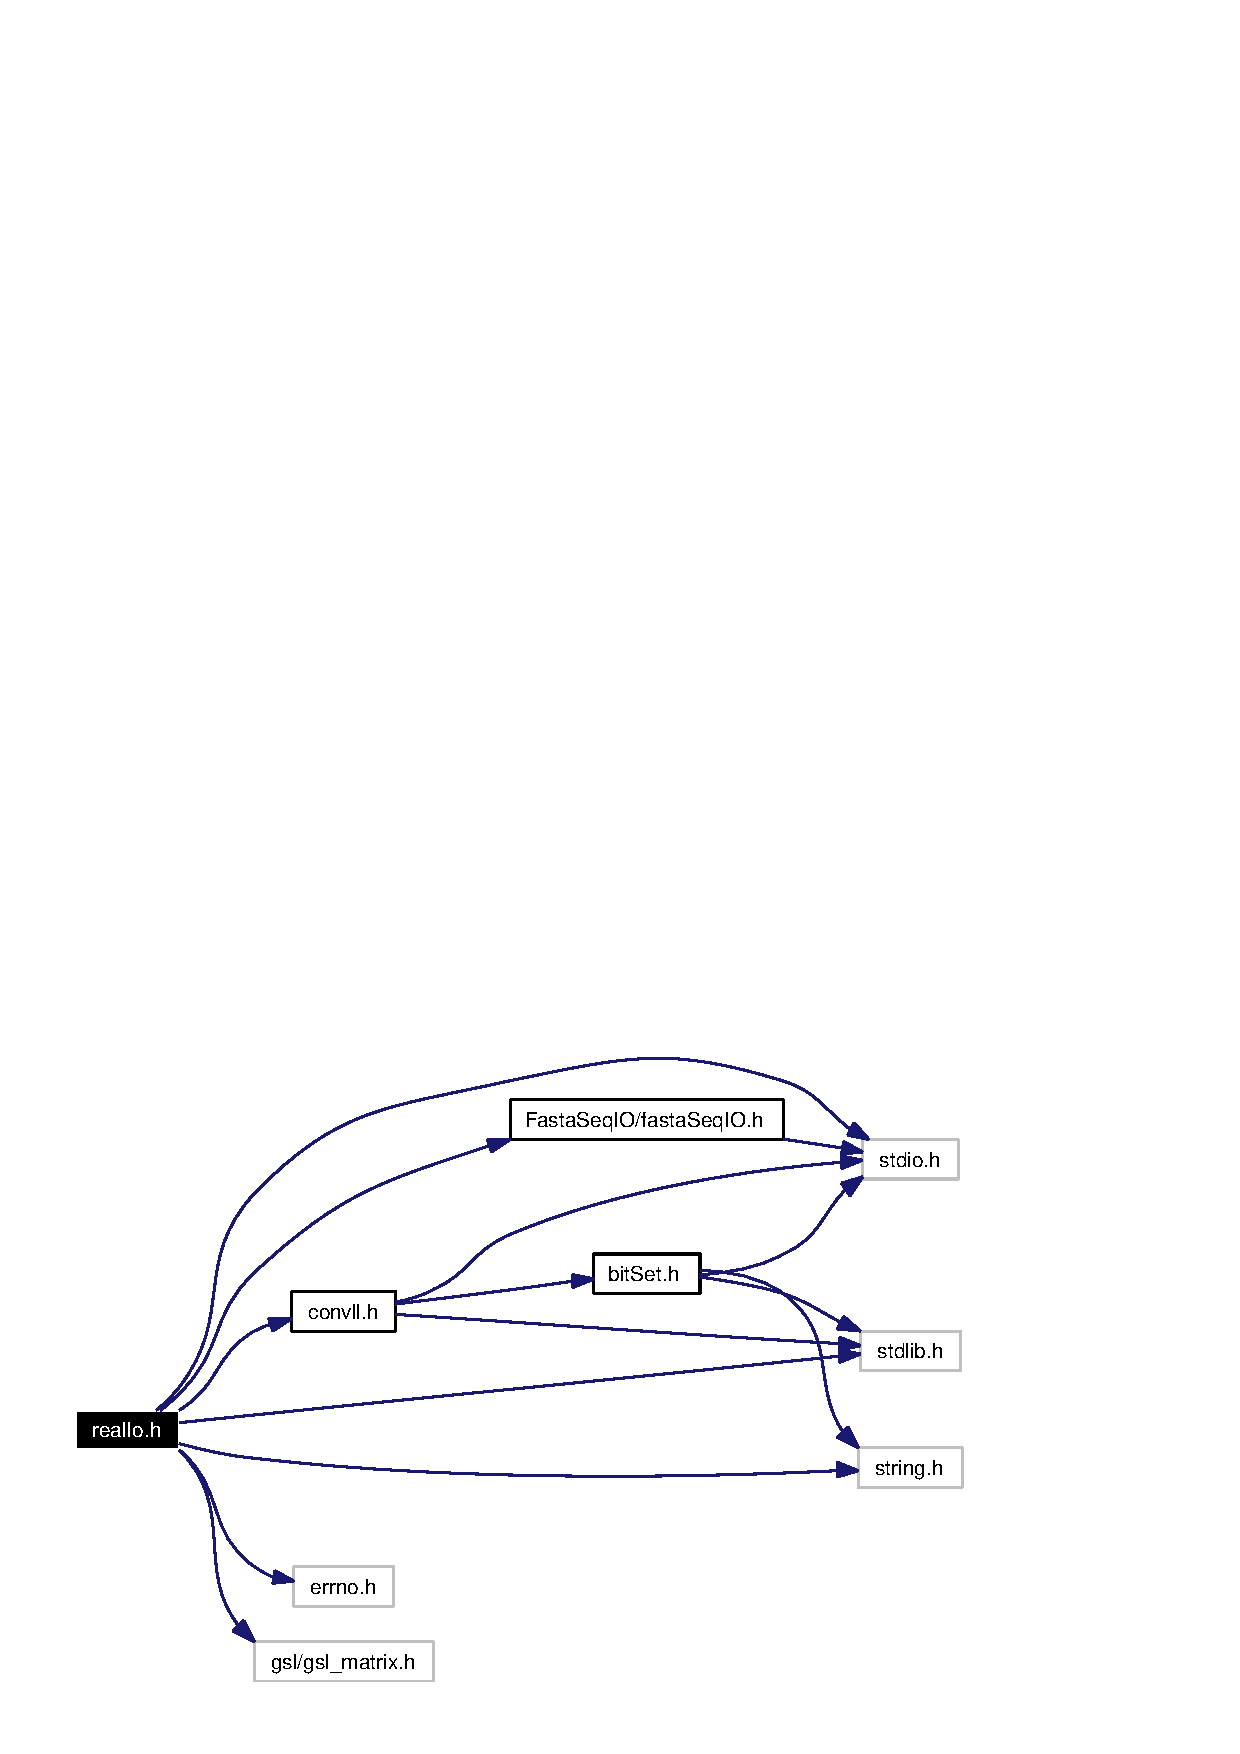
\includegraphics[width=231pt]{realIo_8h__incl}
\end{center}
\end{figure}


This graph shows which files directly or indirectly include this file:\begin{figure}[H]
\begin{center}
\leavevmode
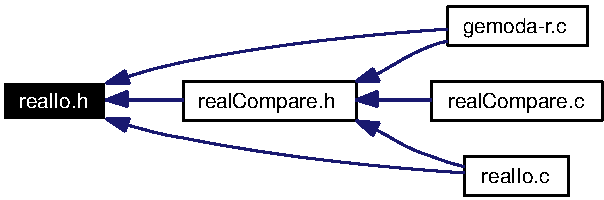
\includegraphics[width=162pt]{realIo_8h__dep__incl}
\end{center}
\end{figure}
\subsection*{Data Structures}
\begin{CompactItemize}
\item 
struct \hyperlink{structrdh__t}{rdh\_\-t}
\end{CompactItemize}
\subsection*{Functions}
\begin{CompactItemize}
\item 
\hyperlink{structrdh__t}{rdh\_\-t} $\ast$ \hyperlink{realIo_8h_a0}{read\-Real\-Data} (FILE $\ast$INPUT)
\item 
\hyperlink{structrdh__t}{rdh\_\-t} $\ast$ \hyperlink{realIo_8h_a1}{free\-Rdh} (\hyperlink{structrdh__t}{rdh\_\-t} $\ast$data)
\item 
int \hyperlink{realIo_8h_a2}{init\-Rdh\-Index} (\hyperlink{structrdh__t}{rdh\_\-t} $\ast$data, int word\-Size, int seq\-Gap)
\item 
int \hyperlink{realIo_8h_a3}{get\-Rdh\-Index\-Seq\-Pos} (\hyperlink{structrdh__t}{rdh\_\-t} $\ast$data, int index, int $\ast$seq, int $\ast$pos)
\item 
int \hyperlink{realIo_8h_a4}{get\-Rdh\-Dim} (\hyperlink{structrdh__t}{rdh\_\-t} $\ast$data)
\item 
int \hyperlink{realIo_8h_a5}{output\-Real\-Pats} (\hyperlink{structrdh__t}{rdh\_\-t} $\ast$data, \hyperlink{structcnode}{cll\_\-t} $\ast$all\-Pats, int L, FILE $\ast$OUTPUT\_\-FILE, int $\ast$$\ast$d)
\item 
int \hyperlink{realIo_8h_a6}{output\-Real\-Pats\-WCentroid} (\hyperlink{structrdh__t}{rdh\_\-t} $\ast$data, \hyperlink{structcnode}{cll\_\-t} $\ast$all\-Pats, int L, FILE $\ast$OUTPUT\_\-FILE, double $\ast$extra\-Params, int comp\-Func)
\end{CompactItemize}


\subsection*{Function Documentation}
\hypertarget{realIo_8h_a1}{
\index{realIo.h@{real\-Io.h}!freeRdh@{freeRdh}}
\index{freeRdh@{freeRdh}!realIo.h@{real\-Io.h}}
\subsubsection[freeRdh]{\setlength{\rightskip}{0pt plus 5cm}\hyperlink{structrdh__t}{rdh\_\-t}$\ast$ free\-Rdh (\hyperlink{structrdh__t}{rdh\_\-t} $\ast$ {\em data})}}
\label{realIo_8h_a1}


This function returns a null pointer after freeing the memory associated with a real data holder object. The function takes one parameter: a pointer to the real data holder, {\em data\/}.

Definition at line 396 of file real\-Io.c.

References rdh\_\-t::index\-To\-Pos, rdh\_\-t::index\-To\-Seq, rdh\_\-t::label, rdh\_\-t::offset\-To\-Index, rdh\_\-t::seq, and rdh\_\-t::size.

Referenced by main().



\hypertarget{realIo_8h_a4}{
\index{realIo.h@{real\-Io.h}!getRdhDim@{getRdhDim}}
\index{getRdhDim@{getRdhDim}!realIo.h@{real\-Io.h}}
\subsubsection[getRdhDim]{\setlength{\rightskip}{0pt plus 5cm}int get\-Rdh\-Dim (\hyperlink{structrdh__t}{rdh\_\-t} $\ast$ {\em data})}}
\label{realIo_8h_a4}


This function returns an integer equal to the dimensions of the data stored in a real data holder object. The function takes one parameter: a pointer to the real data holder, {\em data\/}.

Definition at line 447 of file real\-Io.c.

References rdh\_\-t::seq.

Referenced by general\-Match\-Factor(), get\-Rdh\-Value(), mass\-Spec\-Compare\-WElut(), print\-Rdh\-Seq(), rmsd\-Compare(), and set\-Rdh\-Value().



\hypertarget{realIo_8h_a3}{
\index{realIo.h@{real\-Io.h}!getRdhIndexSeqPos@{getRdhIndexSeqPos}}
\index{getRdhIndexSeqPos@{getRdhIndexSeqPos}!realIo.h@{real\-Io.h}}
\subsubsection[getRdhIndexSeqPos]{\setlength{\rightskip}{0pt plus 5cm}int get\-Rdh\-Index\-Seq\-Pos (\hyperlink{structrdh__t}{rdh\_\-t} $\ast$ {\em data}, int {\em index}, int $\ast$ {\em seq}, int $\ast$ {\em pos})}}
\label{realIo_8h_a3}


This function is used to access and change the sequence and position values, given an index. The function takes four parameters: a pointer to the real data holder, {\em data\/}, an integer {\em index\/}, a pointer integer {\em seq\/}, and a pointer integer {\em pos\/}.

Definition at line 544 of file real\-Io.c.

References rdh\_\-t::index\-Size, rdh\_\-t::index\-To\-Pos, and rdh\_\-t::index\-To\-Seq.

Referenced by general\-Match\-Factor(), make\-Alternate\-Centroid(), mass\-Spec\-Compare\-WElut(), output\-Real\-Pats(), output\-Real\-Pats\-WCentroid(), real\-Comparison(), and rmsd\-Compare().



\hypertarget{realIo_8h_a2}{
\index{realIo.h@{real\-Io.h}!initRdhIndex@{initRdhIndex}}
\index{initRdhIndex@{initRdhIndex}!realIo.h@{real\-Io.h}}
\subsubsection[initRdhIndex]{\setlength{\rightskip}{0pt plus 5cm}int init\-Rdh\-Index (\hyperlink{structrdh__t}{rdh\_\-t} $\ast$ {\em data}, int {\em word\-Size}, int {\em seq\-Gap})}}
\label{realIo_8h_a2}


This function is used to initialize the two indices inside a real data holder. The function takes as its input three parameters a pointer to the real data holder, {\em data\/}, the size of the words to be compared during the comparison stage {\em word\-Size\/}, and an integer {\em seq\-Gap\/}, which is used to place empty data between unique sequences, such that we do not convolve from one sequence into another during the convolution stage.

Definition at line 307 of file real\-Io.c.

References get\-Rdh\-Seq\-Length(), rdh\_\-t::index\-Size, rdh\_\-t::index\-To\-Pos, rdh\_\-t::index\-To\-Seq, rdh\_\-t::offset\-To\-Index, and rdh\_\-t::size.

Referenced by real\-Comparison().



\hypertarget{realIo_8h_a5}{
\index{realIo.h@{real\-Io.h}!outputRealPats@{outputRealPats}}
\index{outputRealPats@{outputRealPats}!realIo.h@{real\-Io.h}}
\subsubsection[outputRealPats]{\setlength{\rightskip}{0pt plus 5cm}int output\-Real\-Pats (\hyperlink{structrdh__t}{rdh\_\-t} $\ast$ {\em data}, \hyperlink{structcnode}{cll\_\-t} $\ast$ {\em all\-Pats}, int {\em L}, FILE $\ast$ {\em OUTPUT\_\-FILE}, int $\ast$$\ast$ {\em d})}}
\label{realIo_8h_a5}


This function is used to print out motifs discovered by Gemoda in an attractive fashion. The function takes five parameters: a pointer to a real data holder object {\em data\/}; a pointer to a linked list of motifs {\em all\-Pats\/}; an integer which is Gemoda's input parameter {\em L\/}; and a pointer to a file handle to which output is printed {\em OUTPUT\_\-FILE\/}.

Definition at line 904 of file real\-Io.c.

References get\-Rdh\-Index\-Seq\-Pos(), cnode::length, c\-Set\_\-t::members, cnode::next, rdh\_\-t::seq, cnode::set, c\-Set\_\-t::size, and cnode::stat.

Referenced by main().



\hypertarget{realIo_8h_a6}{
\index{realIo.h@{real\-Io.h}!outputRealPatsWCentroid@{outputRealPatsWCentroid}}
\index{outputRealPatsWCentroid@{outputRealPatsWCentroid}!realIo.h@{real\-Io.h}}
\subsubsection[outputRealPatsWCentroid]{\setlength{\rightskip}{0pt plus 5cm}int output\-Real\-Pats\-WCentroid (\hyperlink{structrdh__t}{rdh\_\-t} $\ast$ {\em data}, \hyperlink{structcnode}{cll\_\-t} $\ast$ {\em all\-Pats}, int {\em L}, FILE $\ast$ {\em OUTPUT\_\-FILE}, double $\ast$ {\em extra\-Params}, int {\em comp\-Func})}}
\label{realIo_8h_a6}


This function is used to output real valued patterns in a format such that they are centered on a particular centroid.

Definition at line 1068 of file real\-Io.c.

References find\-Clique\-Centroid(), get\-Comp\-Func, get\-Rdh\-Index\-Seq\-Pos(), cnode::length, make\-Alternate\-Centroid(), c\-Set\_\-t::members, cnode::next, cnode::set, and c\-Set\_\-t::size.

Referenced by main().



\hypertarget{realIo_8h_a0}{
\index{realIo.h@{real\-Io.h}!readRealData@{readRealData}}
\index{readRealData@{readRealData}!realIo.h@{real\-Io.h}}
\subsubsection[readRealData]{\setlength{\rightskip}{0pt plus 5cm}\hyperlink{structrdh__t}{rdh\_\-t}$\ast$ read\-Real\-Data (FILE $\ast$ {\em INPUT})}}
\label{realIo_8h_a0}


This function is used to read in a fasta formatted file containing real value data and store the entire thing and a real data holder object. The function takes one parameter: a pointer to a file handle, which is where the data are read from {\em INPUT\/};

Definition at line 850 of file real\-Io.c.

References check\-Real\-Data\-Format(), parse\-Real\-Data(), and Read\-File().

Referenced by main().




\hypertarget{spat_8h}{
\section{spat.h File Reference}
\label{spat_8h}\index{spat.h@{spat.h}}
}


This graph shows which files directly or indirectly include this file:\begin{figure}[H]
\begin{center}
\leavevmode
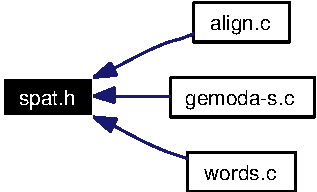
\includegraphics[width=93pt]{spat_8h__dep__incl}
\end{center}
\end{figure}
\subsection*{Data Structures}
\begin{CompactItemize}
\item 
struct \hyperlink{structsOffset__t}{s\-Offset\_\-t}
\item 
struct \hyperlink{structsPat__t}{s\-Pat\_\-t}
\end{CompactItemize}

\hypertarget{words_8c}{
\section{words.c File Reference}
\label{words_8c}\index{words.c@{words.c}}
}
{\tt \#include $<$stdio.h$>$}\par
{\tt \#include $<$stdlib.h$>$}\par
{\tt \#include $<$string.h$>$}\par
{\tt \#include $<$errno.h$>$}\par
{\tt \#include \char`\"{}spat.h\char`\"{}}\par
{\tt \#include \char`\"{}Fasta\-Seq\-IO/fasta\-Seq\-IO.h\char`\"{}}\par


Include dependency graph for words.c:\begin{figure}[H]
\begin{center}
\leavevmode
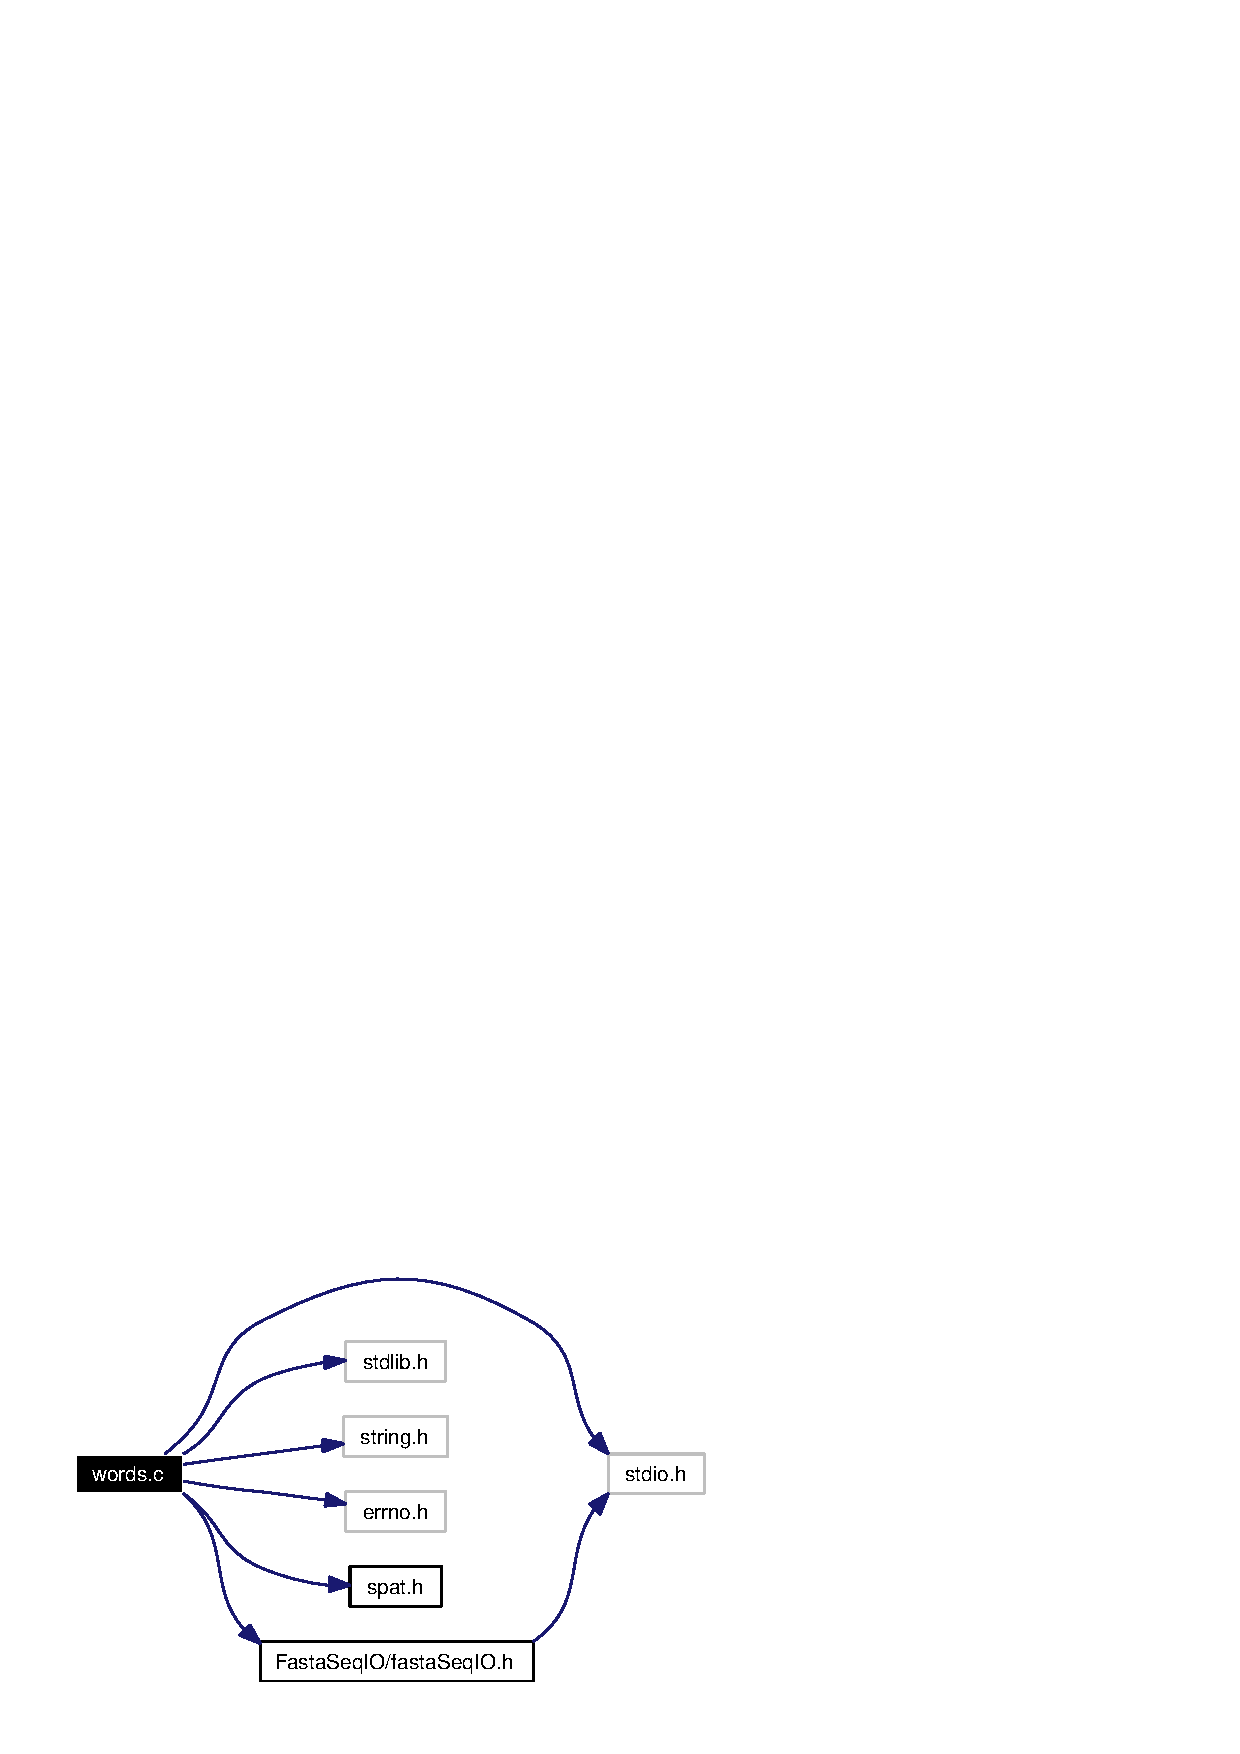
\includegraphics[width=169pt]{words_8c__incl}
\end{center}
\end{figure}
\subsection*{Data Structures}
\begin{CompactItemize}
\item 
struct \hyperlink{structsHashEntry__t}{s\-Hash\-Entry\_\-t}
\item 
struct \hyperlink{structsHash__t}{s\-Hash\_\-t}
\end{CompactItemize}
\subsection*{Defines}
\begin{CompactItemize}
\item 
\#define \hyperlink{words_8c_a0}{SHASH\_\-MAX\_\-KEY\_\-SIZE}~1000
\end{CompactItemize}
\subsection*{Functions}
\begin{CompactItemize}
\item 
int \hyperlink{words_8c_a1}{sieve3} (long n)
\item 
unsigned long \hyperlink{words_8c_a2}{hash1} (unsigned char $\ast$str)
\item 
int \hyperlink{words_8c_a3}{hashpjw} (char $\ast$s)
\item 
\hyperlink{structsHash__t}{s\-Hash\_\-t} \hyperlink{words_8c_a4}{init\-SHash} (int n)
\item 
\hyperlink{structsHashEntry__t}{s\-Hash\-Entry\_\-t} $\ast$ \hyperlink{words_8c_a5}{search\-SHash} (\hyperlink{structsHashEntry__t}{s\-Hash\-Entry\_\-t} $\ast$new\-Entry, \hyperlink{structsHash__t}{s\-Hash\_\-t} $\ast$this\-Hash, int create)
\item 
int \hyperlink{words_8c_a6}{destroy\-SHash} (\hyperlink{structsHash__t}{s\-Hash\_\-t} $\ast$this\-Hash)
\item 
int \hyperlink{words_8c_a7}{print\-SHash} (\hyperlink{structsHash__t}{s\-Hash\_\-t} $\ast$this\-Hash, FILE $\ast$FH)
\item 
int \hyperlink{words_8c_a8}{print\-SPats} (\hyperlink{structsPat__t}{s\-Pat\_\-t} $\ast$a, int n)
\item 
int \hyperlink{words_8c_a9}{destroy\-SPat\-A} (\hyperlink{structsPat__t}{s\-Pat\_\-t} $\ast$words, int wc)
\item 
\hyperlink{structsPat__t}{s\-Pat\_\-t} $\ast$ \hyperlink{words_8c_a10}{count\-Words2} (\hyperlink{structfSeq__t}{f\-Seq\_\-t} $\ast$seq, int num\-Seq, int L, int $\ast$num\-Words)
\end{CompactItemize}


\subsection*{Detailed Description}
This file defines functions that are used in the processing of string based sequences. There are a number of functions defined in this file better used for hashing strings so that the comparison phase can be sped up by only comparing unique words. Heuristically, we have noticed that for sequences in which there is a large degree of redundancy these hashing functions can significantly speed up the comparison phase.

Definition in file \hyperlink{words_8c-source}{words.c}.

\subsection*{Define Documentation}
\hypertarget{words_8c_a0}{
\index{words.c@{words.c}!SHASH_MAX_KEY_SIZE@{SHASH\_\-MAX\_\-KEY\_\-SIZE}}
\index{SHASH_MAX_KEY_SIZE@{SHASH\_\-MAX\_\-KEY\_\-SIZE}!words.c@{words.c}}
\subsubsection[SHASH\_\-MAX\_\-KEY\_\-SIZE]{\setlength{\rightskip}{0pt plus 5cm}\#define SHASH\_\-MAX\_\-KEY\_\-SIZE~1000}}
\label{words_8c_a0}




Definition at line 192 of file words.c.

Referenced by print\-SHash(), and search\-SHash().

\subsection*{Function Documentation}
\hypertarget{words_8c_a10}{
\index{words.c@{words.c}!countWords2@{countWords2}}
\index{countWords2@{countWords2}!words.c@{words.c}}
\subsubsection[countWords2]{\setlength{\rightskip}{0pt plus 5cm}\hyperlink{structsPat__t}{s\-Pat\_\-t}$\ast$ count\-Words2 (\hyperlink{structfSeq__t}{f\-Seq\_\-t} $\ast$ {\em seq}, int {\em num\-Seq}, int {\em L}, int $\ast$ {\em num\-Words})}}
\label{words_8c_a10}


Counts words of size {\em L\/} in the input Fast\-A sequences, hashes all of the words, and returns an array of \hyperlink{structsPat__t}{s\-Pat\_\-t} objects.

Definition at line 373 of file words.c.

References s\-Hash\-Entry\_\-t::data, destroy\-SHash(), s\-Hash\-Entry\_\-t::idx, init\-SHash(), s\-Hash\-Entry\_\-t::key, s\-Hash\-Entry\_\-t::L, s\-Pat\_\-t::length, s\-Offset\_\-t::next, s\-Pat\_\-t::offset, s\-Offset\_\-t::pos, s\-Offset\_\-t::prev, search\-SHash(), s\-Offset\_\-t::seq, sieve3(), s\-Pat\_\-t::string, and s\-Pat\_\-t::support.

Referenced by main().

\scriptsize\begin{verbatim}374 {
375   int i, j;
376   int totalChars = 0;
377   int hashSize;
378   sHashEntry_t newEntry;
379   sHashEntry_t *ep;
380   sHash_t wordHash;
381   sPat_t *words = NULL;
382   int wc = 0;
383   int prev = -1;
384   int l;
385 
386 
387   // Count the total number of characters.  This
388   // is the upper limit on how many words we can have
389   for (i = 0; i < numSeq; i++)
390     {
391       totalChars += strlen (seq[i].seq);
392     }
393 
394   // Get a prime number for the size of the hash table
395   hashSize = sieve3 ((long) (2 * totalChars));
396   wordHash = initSHash (hashSize);
397 
398   // Chop up each sequence and hash out the words of size L
399   for (i = 0; i < numSeq; i++)
400     {
401       prev = -1;
402 
403       // skip sequences that are too short to have
404       // a pattern
405       if (strlen (seq[i].seq) < L)
406     {
407       continue;
408     }
409       for (j = 0; j < strlen (seq[i].seq) - L + 1; j++)
410     {
411 
412       // Make a hash table entry for this word
413       newEntry.key = &(seq[i].seq[j]);
414       newEntry.data = 1;
415       newEntry.idx = wc;
416       newEntry.L = L;
417 
418       // Check to see if it's already in the hash table
419       ep = searchSHash (&newEntry, &wordHash, 0);
420       if (ep == NULL)
421         {
422 
423           // If it's not, create an entry for it
424           ep = searchSHash (&newEntry, &wordHash, 1);
425 
426           // Increase the size of our word array
427           words = (sPat_t *) realloc (words, (wc + 1) * sizeof (sPat_t));
428           if (words == NULL)
429         {
430           fprintf (stderr, "Error!\n");
431           fflush (stderr);
432         }
433           // Add the new word
434           words[wc].string = &(seq[i].seq[j]);
435           words[wc].length = L;
436           words[wc].support = 1;
437           words[wc].offset =
438         (sOffset_t *) malloc (1 * sizeof (sOffset_t));
439           if (words[wc].offset == NULL)
440         {
441           fprintf (stderr, "\nMemory Error\n%s\n", strerror (errno));
442           fflush (stderr);
443           exit (0);
444         }
445           words[wc].offset[0].seq = i;
446           words[wc].offset[0].pos = j;
447           words[wc].offset[0].prev = prev;
448           words[wc].offset[0].next = -1;
449 
450           if (prev != -1)
451         {
452           words[prev].offset[words[prev].support - 1].next = wc;
453         }
454           prev = wc;
455           wc++;
456 
457         }
458       else
459         {
460 
461           // If it is, increase the count for this word
462           ep->data++;
463 
464           // add a new offset to the word array
465           l = words[ep->idx].support;
466           words[ep->idx].offset =
467         (sOffset_t *) realloc (words[ep->idx].offset,
468                        (l + 1) * sizeof (sOffset_t));
469           words[ep->idx].offset[l].seq = i;
470           words[ep->idx].offset[l].pos = j;
471           words[ep->idx].offset[l].prev = prev;
472           words[ep->idx].offset[l].next = -1;
473 
474           // Update the next/prev
475           if (prev != -1)
476         {
477           words[prev].offset[words[prev].support - 1].next = ep->idx;
478         }
479           prev = ep->idx;
480 
481           // Have to put this down here for cases when we create
482           // a word and it is immeadiately followed by itself!!
483           words[ep->idx].support += 1;
484         }
485     }
486     }
487 
488 
489   destroySHash (&wordHash);
490   *numWords = wc;
491   return words;
492 }
\end{verbatim}
\normalsize 


\hypertarget{words_8c_a6}{
\index{words.c@{words.c}!destroySHash@{destroySHash}}
\index{destroySHash@{destroySHash}!words.c@{words.c}}
\subsubsection[destroySHash]{\setlength{\rightskip}{0pt plus 5cm}int destroy\-SHash (\hyperlink{structsHash__t}{s\-Hash\_\-t} $\ast$ {\em this\-Hash})}}
\label{words_8c_a6}


Destroy a hash table, freeing the memory.

Definition at line 272 of file words.c.

References s\-Hash\_\-t::hash, s\-Hash\_\-t::hash\-Size, and s\-Hash\_\-t::i\-Hash\-Size.

Referenced by count\-Words2().

\scriptsize\begin{verbatim}273 {
274   int i;
275   free (thisHash->iHashSize);
276   free (thisHash->hashSize);
277   for (i = 0; i < thisHash->totalSize; i++)
278     {
279       if (thisHash->hash[i] != NULL)
280     {
281       free (thisHash->hash[i]);
282       thisHash->hash[i] = NULL;
283     }
284     }
285   if (thisHash->hash != NULL)
286     {
287       free (thisHash->hash);
288       thisHash->hash = NULL;
289     }
290   return 0;
291 }
\end{verbatim}
\normalsize 


\hypertarget{words_8c_a9}{
\index{words.c@{words.c}!destroySPatA@{destroySPatA}}
\index{destroySPatA@{destroySPatA}!words.c@{words.c}}
\subsubsection[destroySPatA]{\setlength{\rightskip}{0pt plus 5cm}int destroy\-SPat\-A (\hyperlink{structsPat__t}{s\-Pat\_\-t} $\ast$ {\em words}, int {\em wc})}}
\label{words_8c_a9}


This function is used to free up the memory allocated in an array of \hyperlink{structsPat__t}{s\-Pat\_\-t} space objects. The function returns a null pointer.

Definition at line 352 of file words.c.

References s\-Pat\_\-t::offset.

\scriptsize\begin{verbatim}353 {
354   int i;
355   for (i = 0; i < wc; i++)
356     {
357       if (words[i].offset != NULL)
358     {
359       free (words[i].offset);
360       words[i].offset = NULL;
361     }
362     }
363   free (words);
364   words = NULL;
365   return 0;
366 }
\end{verbatim}
\normalsize 


\hypertarget{words_8c_a2}{
\index{words.c@{words.c}!hash1@{hash1}}
\index{hash1@{hash1}!words.c@{words.c}}
\subsubsection[hash1]{\setlength{\rightskip}{0pt plus 5cm}unsigned long hash1 (unsigned char $\ast$ {\em str})}}
\label{words_8c_a2}


A hashing function that returns an integer, given a pointer to a null characterterminated string.

Definition at line 73 of file words.c.

Referenced by search\-SHash().

\scriptsize\begin{verbatim}74 {
75   unsigned long hash = 5381;
76   int c;
77 
78   while ((c = *str++))
79     hash = ((hash << 5) + hash) + c;    /* hash * 33 + c */
80 
81   return hash;
82 }
\end{verbatim}
\normalsize 


\hypertarget{words_8c_a3}{
\index{words.c@{words.c}!hashpjw@{hashpjw}}
\index{hashpjw@{hashpjw}!words.c@{words.c}}
\subsubsection[hashpjw]{\setlength{\rightskip}{0pt plus 5cm}int hashpjw (char $\ast$ {\em s})}}
\label{words_8c_a3}


A hashing function that returns an integer, given a pointer to a null characterterminated string.

Definition at line 89 of file words.c.

\scriptsize\begin{verbatim}90 {
91   char *p;
92   unsigned int h, g;
93 
94   h = 0;
95   for (p = s; *p != '\0'; p++)
96     {
97       h = (h << 4) + *p;
98       if ((g = h & 0xF0000000))
99     {
100       h ^= g >> 24;
101       h ^= g;
102     }
103     }
104   return h;
105 }
\end{verbatim}
\normalsize 


\hypertarget{words_8c_a4}{
\index{words.c@{words.c}!initSHash@{initSHash}}
\index{initSHash@{initSHash}!words.c@{words.c}}
\subsubsection[initSHash]{\setlength{\rightskip}{0pt plus 5cm}\hyperlink{structsHash__t}{s\-Hash\_\-t} init\-SHash (int {\em n})}}
\label{words_8c_a4}


Allocates the memory for a s\-Hash table and initializes some of the elements.

Definition at line 155 of file words.c.

References s\-Hash\_\-t::total\-Size.

Referenced by count\-Words2().

\scriptsize\begin{verbatim}156 {
157   int i = 0;
158   int step = 0;
159   sHash_t this;
160 
161   this.totalSize = n;
162   this.hashSize = (int *) malloc (n * sizeof (int));
163   if (this.hashSize == NULL)
164     {
165       fprintf (stderr, "\nMemory Error\n%s\n", strerror (errno));
166       fflush (stderr);
167       exit (0);
168     }
169   this.iHashSize = (int *) malloc (n * sizeof (int));
170   if (this.iHashSize == NULL)
171     {
172       fprintf (stderr, "\nMemory Error\n%s\n", strerror (errno));
173       fflush (stderr);
174       exit (0);
175     }
176   this.hash = (sHashEntry_t **) malloc (n * sizeof (sHashEntry_t *));
177   if (this.hash == NULL)
178     {
179       fprintf (stderr, "\nMemory Error\n%s\n", strerror (errno));
180       fflush (stderr);
181       exit (0);
182     }
183   for (i = 0; i < n; i++)
184     {
185       this.hash[i] = NULL;
186       this.hashSize[i] = 0;
187       this.iHashSize[i] = step;
188     }
189   return this;
190 }
\end{verbatim}
\normalsize 


\hypertarget{words_8c_a7}{
\index{words.c@{words.c}!printSHash@{printSHash}}
\index{printSHash@{printSHash}!words.c@{words.c}}
\subsubsection[printSHash]{\setlength{\rightskip}{0pt plus 5cm}int print\-SHash (\hyperlink{structsHash__t}{s\-Hash\_\-t} $\ast$ {\em this\-Hash}, FILE $\ast$ {\em FH})}}
\label{words_8c_a7}


This function is used to print the hash out and is generally only used for error checking.

Definition at line 298 of file words.c.

References s\-Hash\-Entry\_\-t::data, s\-Hash\_\-t::hash, s\-Hash\-Entry\_\-t::key, s\-Hash\-Entry\_\-t::L, and SHASH\_\-MAX\_\-KEY\_\-SIZE.

\scriptsize\begin{verbatim}299 {
300   int i, j;
301   char string[SHASH_MAX_KEY_SIZE];
302 
303   for (i = 0; i < thisHash->totalSize; i++)
304     {
305       for (j = 0; j < thisHash->hashSize[i]; j++)
306     {
307 
308       strncpy (string, thisHash->hash[i][j].key, thisHash->hash[i][j].L);
309       string[thisHash->hash[i][j].L] = '\0';
310       fprintf (FH, "%s %d\n", string, thisHash->hash[i][j].data);
311 
312     }
313     }
314   return 0;
315 }
\end{verbatim}
\normalsize 


\hypertarget{words_8c_a8}{
\index{words.c@{words.c}!printSPats@{printSPats}}
\index{printSPats@{printSPats}!words.c@{words.c}}
\subsubsection[printSPats]{\setlength{\rightskip}{0pt plus 5cm}int print\-SPats (\hyperlink{structsPat__t}{s\-Pat\_\-t} $\ast$ {\em a}, int {\em n})}}
\label{words_8c_a8}


This function is used to print out an array of \hyperlink{structsPat__t}{s\-Pat\_\-t} objects and is generally only used for error checking.

Definition at line 321 of file words.c.

References s\-Pat\_\-t::length.

\scriptsize\begin{verbatim}322 {
323   char *s = NULL;
324   int i, j;
325   int size = 0;
326   for (i = 0; i < n; i++)
327     {
328       if (a[i].length > size)
329     {
330       s = (char *) realloc (s, a[i].length * sizeof (char));
331     }
332       strncpy (s, a[i].string, a[i].length);
333       s[a[i].length] = '\0';
334       printf ("%d:  %s\n", i, s);
335       for (j = 0; j < a[i].support; j++)
336     {
337       printf ("\t%d %d -> (%d, %d)\n", a[i].offset[j].seq,
338           a[i].offset[j].pos, a[i].offset[j].prev,
339           a[i].offset[j].next);
340     }
341       printf ("\n");
342     }
343   free (s);
344   return 0;
345 }
\end{verbatim}
\normalsize 


\hypertarget{words_8c_a5}{
\index{words.c@{words.c}!searchSHash@{searchSHash}}
\index{searchSHash@{searchSHash}!words.c@{words.c}}
\subsubsection[searchSHash]{\setlength{\rightskip}{0pt plus 5cm}\hyperlink{structsHashEntry__t}{s\-Hash\-Entry\_\-t}$\ast$ search\-SHash (\hyperlink{structsHashEntry__t}{s\-Hash\-Entry\_\-t} $\ast$ {\em new\-Entry}, \hyperlink{structsHash__t}{s\-Hash\_\-t} $\ast$ {\em this\-Hash}, int {\em create})}}
\label{words_8c_a5}


This function has two purposes. It searches for entries in the hash table and it puts new entries in.

Definition at line 198 of file words.c.

References s\-Hash\_\-t::hash, hash1(), s\-Hash\_\-t::hash\-Size, s\-Hash\_\-t::i\-Hash\-Size, s\-Hash\-Entry\_\-t::key, s\-Hash\-Entry\_\-t::L, SHASH\_\-MAX\_\-KEY\_\-SIZE, and s\-Hash\_\-t::total\-Size.

Referenced by count\-Words2().

\scriptsize\begin{verbatim}199 {
200   char string[SHASH_MAX_KEY_SIZE];
201   unsigned long (*hashFunction) () = &hash1;
202   int i, thisIndex;
203   int status = 0;
204 
205   // A string to store the key
206   strncpy (string, newEntry->key, newEntry->L);
207   string[newEntry->L] = '\0';
208 
209   // The index that this key hashes to
210   thisIndex = hashFunction ((unsigned char *) string) % thisHash->totalSize;
211 
212   // For each member that has this index, check to see
213   // if the key is the same
214   for (i = 0; i < thisHash->hashSize[thisIndex]; i++)
215     {
216       if (strncmp (thisHash->hash[thisIndex][i].key, string, newEntry->L) ==
217       0)
218     {
219 
220       // We found a match
221       /*
222          printf("\t%s already in hash table!\n"); 
223        */
224       status = 1;
225       return &(thisHash->hash[thisIndex][i]);
226       break;
227 
228     }
229     }
230 
231   // If we didn't find the key and we're told to create it,
232   // then allocate new memory for the hashEntry and put it in
233   if (status == 0 && create != 0)
234     {
235 
236       // Allocate space for the new entry at this index
237       if (thisHash->iHashSize[thisIndex] == 0)
238     {
239       thisHash->hash[thisIndex] =
240         (sHashEntry_t *) malloc (sizeof (sHashEntry_t));
241     }
242       else
243     {
244       thisHash->hash[thisIndex] =
245         (sHashEntry_t *) realloc (thisHash->hash[thisIndex],
246                       (thisHash->iHashSize[thisIndex] +
247                        1) * sizeof (sHashEntry_t));
248     }
249       if (thisHash->hash[thisIndex] == NULL)
250     {
251       fprintf (stderr, "\nMemory Error\n%s\n", strerror (errno));
252       fflush (stderr);
253       exit (0);
254     }
255       // Increase our record of the size
256       i = thisHash->hashSize[thisIndex];
257       thisHash->hash[thisIndex][i] = *newEntry;
258       thisHash->iHashSize[thisIndex]++;
259       thisHash->hashSize[thisIndex]++;
260 
261 
262       // Return a pointer to this entry
263       return &(thisHash->hash[thisIndex][i]);
264     }
265   return NULL;
266 }
\end{verbatim}
\normalsize 


\hypertarget{words_8c_a1}{
\index{words.c@{words.c}!sieve3@{sieve3}}
\index{sieve3@{sieve3}!words.c@{words.c}}
\subsubsection[sieve3]{\setlength{\rightskip}{0pt plus 5cm}int sieve3 (long {\em n})}}
\label{words_8c_a1}


Prime number generator: returns first prime number equal or less than\begin{Desc}
\item[Parameters:]
\begin{description}
\item[{\em n.}]\end{description}
\end{Desc}


Definition at line 27 of file words.c.

Referenced by count\-Words2().

\scriptsize\begin{verbatim}28 {
29   int i, p, j;
30   int *a;
31   a = (int *) malloc ((n + 1) * sizeof (int));
32   if (a == NULL)
33     {
34       fprintf (stderr, "\nMemory Error\n%s\n", strerror (errno));
35       fflush (stderr);
36       exit (0);
37     }
38   a[0] = 0;
39   a[1] = 0;
40   for (i = 2; i < n; i++)
41     {
42       a[i] = 1;
43     }
44   p = 2;
45   do
46     {
47       j = 2 * p;
48       do
49     {
50       a[j] = 0;
51       j = j + p;
52     }
53       while (j <= n);
54       p = p + 1;
55     }
56   while (p * p < 2 * n);
57   for (i = n; i > 2; i--)
58     {
59       if (a[i])
60     {
61       free (a);
62       return i;
63     }
64     }
65   free (a);
66   return 0;
67 }
\end{verbatim}
\normalsize 



\printindex
\end{document}
